%%%%%%%%%%%%%%%%%%%%%%%%%%%%%%%%%%%%%%%%%%%%%%%%%%%%%%%%%%%%%%%
%% OXFORD THESIS TEMPLATE

% Use this template to produce a standard thesis that meets the Oxford University requirements for DPhil submission
%
% Originally by Keith A. Gillow (gillow@maths.ox.ac.uk), 1997
% Modified by Sam Evans (sam@samuelevansresearch.org), 2007
% Modified by John McManigle (john@oxfordechoes.com), 2015
% Modified by Ulrik Lyngs (ulrik.lyngs@cs.ox.ac.uk), 2018, for use with R Markdown
%
% Ulrik Lyngs, 25 Nov 2018: Following John McManigle, broad permissions are granted to use, modify, and distribute this software
% as specified in the MIT License included in this distribution's LICENSE file.
%
% John tried to comment this file extensively, so read through it to see how to use the various options.  Remember
% that in LaTeX, any line starting with a % is NOT executed.  Several places below, you have a choice of which line to use
% out of multiple options (eg draft vs final, for PDF vs for binding, etc.)  When you pick one, add a % to the beginning of
% the lines you don't want.


%%%%% CHOOSE PAGE LAYOUT
% The most common choices should be below.  You can also do other things, like replacing "a4paper" with "letterpaper", etc.

% This one will format for two-sided binding (ie left and right pages have mirror margins; blank pages inserted where needed):
%\documentclass[a4paper,twoside]{templates/ociamthesis}
% This one will format for one-sided binding (ie left margin > right margin; no extra blank pages):
%\documentclass[a4paper]{ociamthesis}
% This one will format for PDF output (ie equal margins, no extra blank pages):
%\documentclass[a4paper,nobind]{templates/ociamthesis}
%UL 2 Dec 2018: pass this in from YAML
\documentclass[a4paper, nobind]{templates/ociamthesis}


% UL 30 Nov 2018 pandoc puts lists in 'tightlist' command when no space between bullet points in Rmd file
\providecommand{\tightlist}{%
  \setlength{\itemsep}{0pt}\setlength{\parskip}{0pt}}
 
% UL 1 Dec 2018, fix to include code in shaded environments

%UL 2 Dec 2018 reduce whitespace around verbatim environments
\usepackage{etoolbox}
\makeatletter
\preto{\@verbatim}{\topsep=0pt \partopsep=0pt }
\makeatother

%UL 26 Mar 2019, enable strikethrough
\usepackage[normalem]{ulem}

%UL 15 Oct 2019, enable link highlighting to be turned off from YAML
\usepackage[colorlinks=false,pdfpagelabels,hidelinks=true]{hyperref}

%%%%% SELECT YOUR DRAFT OPTIONS
% Three options going on here; use in any combination.  But remember to turn the first two off before
% generating a PDF to send to the printer!

% This adds a "DRAFT" footer to every normal page.  (The first page of each chapter is not a "normal" page.)

% This highlights (in blue) corrections marked with (for words) \mccorrect{blah} or (for whole
% paragraphs) \begin{mccorrection} . . . \end{mccorrection}.  This can be useful for sending a PDF of
% your corrected thesis to your examiners for review.  Turn it off, and the blue disappears.
\correctionstrue

%%%%% BIBLIOGRAPHY SETUP
% Note that your bibliography will require some tweaking depending on your department, preferred format, etc.
% The options included below are just very basic "sciencey" and "humanitiesey" options to get started.
% If you've not used LaTeX before, I recommend reading a little about biblatex/biber and getting started with it.
% If you're already a LaTeX pro and are used to natbib or something, modify as necessary.
% Either way, you'll have to choose and configure an appropriate bibliography format...

% The science-type option: numerical in-text citation with references in order of appearance.
% \usepackage[style=numeric-comp, sorting=none, backend=biber, doi=false, isbn=false]{biblatex}
% \newcommand*{\bibtitle}{References}

% The humanities-type option: author-year in-text citation with an alphabetical works cited.
% \usepackage[style=authoryear, sorting=nyt, backend=biber, maxcitenames=2, useprefix, doi=false, isbn=false]{biblatex}
% \newcommand*{\bibtitle}{Works Cited}

%UL 3 Dec 2018: set this from YAML in index.Rmd
% \usepackage[style=authoryear, sorting=nyt, backend=biber, maxcitenames=2, mincitenames=1, useprefix, doi=false, isbn=false, url=false, eprint=false, dashed=false, uniquename=false]{biblatex}
\usepackage[backend=biber,
    bibencoding=utf8,
    refsection=chapter,
    style=authoryear, 
    firstinits=true,
    isbn=false,
    doi=true,
    url=false,
    eprint=false,
    related=false,
    dashed=false,
    clearlang=true,
    maxcitenames=2,
    mincitenames=1,
    maxbibnames=10,
    abbreviate=false,
    minbibnames=3,
    uniquelist=minyear,
    sortcites=true,
    date=year
]{biblatex}
\AtEveryBibitem{%
  \clearlist{language}%
  \clearfield{note}
}

\DeclareFieldFormat{titlecase}{\MakeTitleCase{#1}}

\newrobustcmd{\MakeTitleCase}[1]{%
  \ifthenelse{\ifcurrentfield{booktitle}\OR\ifcurrentfield{booksubtitle}%
    \OR\ifcurrentfield{maintitle}\OR\ifcurrentfield{mainsubtitle}%
    \OR\ifcurrentfield{journaltitle}\OR\ifcurrentfield{journalsubtitle}%
    \OR\ifcurrentfield{issuetitle}\OR\ifcurrentfield{issuesubtitle}%
    \OR\ifentrytype{book}\OR\ifentrytype{mvbook}\OR\ifentrytype{bookinbook}%
    \OR\ifentrytype{booklet}\OR\ifentrytype{suppbook}%
    \OR\ifentrytype{collection}\OR\ifentrytype{mvcollection}%
    \OR\ifentrytype{suppcollection}\OR\ifentrytype{manual}%
    \OR\ifentrytype{periodical}\OR\ifentrytype{suppperiodical}%
    \OR\ifentrytype{proceedings}\OR\ifentrytype{mvproceedings}%
    \OR\ifentrytype{reference}\OR\ifentrytype{mvreference}%
    \OR\ifentrytype{report}\OR\ifentrytype{thesis}}
    {#1}
    {\MakeSentenceCase{#1}}}
    
% \renewbibmacro{in:}{}
% suppress "in" for articles
% https://tex.stackexchange.com/questions/10682/suppress-in-biblatex
\renewbibmacro{in:}{%
  \ifentrytype{article}{}{\printtext{\bibstring{in}\intitlepunct}}}
%-- no "quotes" around titles of chapters/article titles
\DeclareFieldFormat[article, inbook, incollection, inproceedings, misc, thesis, unpublished]
{title}{#1}
%-- no punctuation after volume
\DeclareFieldFormat[article]
{volume}{{#1}}
%-- puts number/issue between brackets
\DeclareFieldFormat[article, inbook, incollection, inproceedings, misc, thesis, unpublished]
{number}{\mkbibparens{#1}} 
%-- and then for articles directly the pages w/o any "pages" or "pp." 
\DeclareFieldFormat[article]
{pages}{#1}
%-- for some types replace "pages" by "p."
\DeclareFieldFormat[inproceedings, incollection, inbook]
{pages}{p. #1}
%-- format 16(4):224--225 for articles
\renewbibmacro*{volume+number+eid}{
  \printfield{volume}%
  \printfield{number}%
  \printunit{\addcolon}
}

\newcommand*{\bibtitle}{References}

% This makes the bibliography left-aligned (not 'justified') and slightly smaller font.
\renewcommand*{\bibfont}{\raggedright\small}

% Change this to the name of your .bib file (usually exported from a citation manager like Zotero or EndNote).
\addbibresource{references.bib}


% Uncomment this if you want equation numbers per section (2.3.12), instead of per chapter (2.18):
%\numberwithin{equation}{subsection}


%%%%% THESIS / TITLE PAGE INFORMATION
% Everybody needs to complete the following:
\title{Flexibility in avian\\
migration across scales}
\author{Benjamin Mark Van Doren}
\college{Somerville College}

% Master's candidates who require the alternate title page (with candidate number and word count)
% must also un-comment and complete the following three lines:
%\masterssubmissiontrue
%\candidateno{933516}
%\wordcount{28,815}

% Uncomment the following line if your degree also includes exams (eg most masters):
%\renewcommand{\submittedtext}{Submitted in partial completion of the}
% Your full degree name.  (But remember that DPhils aren't "in" anything.  They're just DPhils.)
\degree{Doctor of Philosophy}
% Term and year of submission, or date if your board requires (eg most masters)
\degreedate{Hilary 2020}


%%%%% YOUR OWN PERSONAL MACROS
% This is a good place to dump your own LaTeX macros as they come up.

% To make text superscripts shortcuts
	\renewcommand{\th}{\textsuperscript{th}} % ex: I won 4\th place
	\newcommand{\nd}{\textsuperscript{nd}}
	\renewcommand{\st}{\textsuperscript{st}}
	\newcommand{\rd}{\textsuperscript{rd}}

%%%%% THE ACTUAL DOCUMENT STARTS HERE
\begin{document}

%%%%% CHOOSE YOUR LINE SPACING HERE
% This is the official option.  Use it for your submission copy and library copy:
\setlength{\textbaselineskip}{22pt plus2pt}
% This is closer spacing (about 1.5-spaced) that you might prefer for your personal copies:
%\setlength{\textbaselineskip}{18pt plus2pt minus1pt}

% You can set the spacing here for the roman-numbered pages (acknowledgements, table of contents, etc.)
\setlength{\frontmatterbaselineskip}{17pt plus1pt minus1pt}
% \setlength{\frontmatterbaselineskip}{16pt plus1pt minus1pt}

% UL: You can set the line and paragraph spacing here for the separate abstract page to be handed in to Examination schools
\setlength{\abstractseparatelineskip}{13pt plus1pt minus1pt}
\setlength{\abstractseparateparskip}{0pt plus 1pt}

% UL: You can set the general paragraph spacing here - I've set it to 2pt (was 0) so
% it's less claustrophobic
\setlength{\parskip}{2pt plus 1pt}


% Leave this line alone; it gets things started for the real document.
\setlength{\baselineskip}{\textbaselineskip}


%%%%% CHOOSE YOUR SECTION NUMBERING DEPTH HERE
% You have two choices.  First, how far down are sections numbered?  (Below that, they're named but
% don't get numbers.)  Second, what level of section appears in the table of contents?  These don't have
% to match: you can have numbered sections that don't show up in the ToC, or unnumbered sections that
% do.  Throughout, 0 = chapter; 1 = section; 2 = subsection; 3 = subsubsection, 4 = paragraph...

% The level that gets a number:
\setcounter{secnumdepth}{2}
% The level that shows up in the ToC:
\setcounter{tocdepth}{0}


%%%%% ABSTRACT SEPARATE
% This is used to create the separate, one-page abstract that you are required to hand into the Exam
% Schools.  You can comment it out to generate a PDF for printing or whatnot.

% JEM: Pages are roman numbered from here, though page numbers are invisible until ToC.  This is in
% keeping with most typesetting conventions.
\begin{romanpages}

% Title page is created here
\maketitle

%%%%% DEDICATION -- If you'd like one, un-comment the following.
\begin{dedication}
  \begin{center}
  
  \begin{tabular}{l}
  
  He’s a birder---briefly, a student of birds---  \\
  Noting those he sees in his mind or his  \\
  camera, items found for collection, the many\\
  made more by research, or his travels.\\\\
  
  They’re his science, he says, telling you, if you \\
  listen, of habits and rarity, but what you see \\
  are the colors and shapes, the moments of \\
  movement he captures, showing themselves. \\\\
  
  Devoted to kinds beyond counting, he includes   \\
  what’s sweet, fierce, often unseen but yet heard,  \\
  the breathtakingly beautiful stars of his sky.  \\\\
  
  \end{tabular}
  
  \vspace{200pt}
  
  From \textit{Birder}, by John Van Doren (1928--2019), \\
  who loved hemlock trees and waterfalls.
  
  \end{center}
\end{dedication}

%%%%% ACKNOWLEDGEMENTS -- Nothing to do here except comment out if you don't want it.
\begin{acknowledgements}
 	I am incredibly fortunate to have had many wonderful mentors during my DPhil. To my Oxford supervisors, Ben Sheldon and Sonya Clegg, thank you for your steadfast guidance, for the freedom you have given me to pursue my ideas and goals, and for always trusting in my ability to accomplish more than I thought possible.

To my ``adjunct supervisor,'' Miriam Liedvogel, I am humbled by your unwavering support. Your boundless generosity, enthusiasm for science, and care for your students never ceases to amaze me.

To Barbara Helm, I am deeply grateful for your guidance and friendship. You have taught me so much about what it means to be a better scientist, collaborator, and person. I will cherish our talks about science and life in between tours of Scottish highlands and Dutch lowlands.

To Andrew Farnsworth, who introduced me to the wonders of bird migration over ten years ago, thank you for sharing your endless enthusiasm and knowledge with me. I can always count on our conversations to remind me why migration is so amazing and motivate me to seek insights and answers. More soon, I am sure!

I have been privileged to work with and learn from many colleagues and collaborators. Thank you to Kyle Horton, Kristen Ruegg, Wesley Hochachka, Dan Sheldon, and many others.

Fieldwork is filled with many challenges, expected and unexpected. I am indebted to a number of people who helped make my blackcap-catching exploits a success. Thank you, Greg, for your insights, guidance, and logistical support. To Keith, thank you for teaching me how to ring a bird and for the many chocolate digestives that got me through cold mornings. To Robbie, thank you for sharing your knowledge, skills, and time, and for your determination and keen intuition in the field. You have been instrumental in making fieldwork as successful as it was. I am grateful to the dozens of ringers who participated in fieldwork, and to the blackcap hosts who opened their homes and gardens to the project and kept an eye out for marked birds. There are too many to name here, but I am especially indebted to Glynne, Graham, Stuart, Lyn, Dee and Jonnie. I received generous support from many others along the way---special thanks to Malcolm Burgess, Kira Delmore, and Nicole Milligan.

My years in Oxford have been some of the best of my life, thanks to the many cherished friends I have made here, especially in the Marshall, Somerville, and Zoology communities.
To Julius, Noam, and Taylor, thank you for making Oxford feel so much like home.

To my wonderful family, thank you for supporting and nourishing my interest in birds and science. To my brother, Ross, whom I once tortured with an ill-advised ``bird school'' and who sat through many avian detours on family trips, thank you for your understanding---and for still being interested in my career. To my grandparents, Mira and John, thank you for your encouragement, excitement, and a lifetime's worth of bird books. Finally, thank you to my parents, Susan and Daniel, who documented my first sentence (``Hello duck!''), bought six-year-old me a field guide to birds, and made possible countless early morning (and late morning, afternoon, and nighttime) excursions as I followed my passion for birds and nature.
\end{acknowledgements}

%%%%% AUTHOR CONTRIBUTIONS -- Nothing to do here except comment out if you don't want it.
\begin{contributions}
 	\textbf{Benjamin Van Doren} had independent intellectual input into all aspects of the thesis. He conducted and oversaw blackcap fieldwork in the UK over four winters, analyzed data for all studies, drafted chapters, and incorporated co-author comments to produce final manuscripts.

\vspace{8pt}

\textbf{Ben C. Sheldon} (supervisor, co-author of chapters \ref{blackcap-geo} and \ref{blackcap-uk}) secured funding and provided intellectual input, guidance, and feedback.

\textbf{Sonya M. Clegg} (supervisor) provided intellectual input, guidance, and feedback.

\textbf{Miriam Liedvogel} (co-author of chapters \ref{stonechats}, \ref{blackcap-geo} and \ref{blackcap-uk}) secured funding and provided intellectual input, guidance, and written contributions for co-authored chapters.

\textbf{Barbara Helm} (co-author of chapters \ref{stonechats} and \ref{flycatchers}) provided intellectual input, guidance, and written contributions for co-authored chapters.

\hypertarget{additional-contributors}{%
\subsubsection{\texorpdfstring{\emph{Additional contributors}}{Additional contributors}}\label{additional-contributors}}

\textbf{Greg J. Conway} (co-author of chapters \ref{blackcap-geo} and \ref{blackcap-uk}) secured funding and helped oversee blackcap fieldwork. Provided guidance and intellectual input for co-authored chapters.

\textbf{Kira Delmore} (co-author of chapter \ref{blackcap-geo}) coordinated and conducted blackcap fieldwork in continental Europe. Contributed data, analysis, and writing to chapter \ref{blackcap-geo}.

\textbf{Andrew Farnsworth} (co-author of chapter \ref{lights}) provided guidance and intellectual input. Contributed oversight and writing to chapter \ref{lights}.

\textbf{Kyle G. Horton} (co-author of chapters \ref{forecast} and \ref{lights}) provided intellectual input, writing, and data analysis for co-authored chapters.

\textbf{Robbie J. Phillips} (co-author of chapters \ref{forecast} and \ref{lights}) assisted with UK fieldwork and provided intellectual input and feedback for co-authored chapters.

\vspace{12pt}

Further author contributions information accompanies each chapter.
\end{contributions}


%%%%% ABSTRACT -- Nothing to do here except comment out if you don't want it.
\begin{abstract}
	Migratory birds form a network of organisms that connect the world, serving as indicators of ecosystem health and biodiversity on a hemispheric scale. Unfortunately, avian migrants are threatened by the rapidly increasing pressures of global change. Understanding the capabilities of migratory birds to respond to established and emerging challenges requires knowledge of the complex interactions among individuals, populations, species, and natural and built environments. In this thesis, I surveyed the drivers of bird migration across scales. I focused on the contributions of the innate migratory program, birds' responses to environmental cues and conditions, and the influence of human activity on migratory behavior.

First, I investigated birds' innate migratory programs. I demonstrated that stonechats (genus \emph{Saxicola}) possess inherited programs that vary among taxa according to migratory tendency, but also readily interact with environmental factors to influence migratory phenotypes (Chapter \ref{stonechats}). Next, I combined field and laboratory studies to show that ongoing responses to climate change in a long-distance migrant, the pied flycatcher (\emph{Ficedula hypoleuca}), involve not only phenotypic plasticity, but microevolutionary change as well (Chapter \ref{flycatchers}). I then shifted to a wild context and examined the migration of the Eurasian blackcap (\emph{Sylvia atricapilla}) across its European range, illustrating two different ways that natural selection can act on migratory strategies (Chapter \ref{blackcap-geo}). Expanding to a continental perspective, I showed that migratory flexibility is important not only on evolutionary timescales, but also to enable short-term responses to variable environmental conditions during active migratory flights---and that these responses are predictable enough to reliably forecast avian movements (Chapter \ref{forecast}). Finally, I focused on human impacts on migration, showing that artificial light at night can drastically affect migratory journeys (Chapter \ref{lights}). Human activity can impact not only migrants' in-flight behaviors, but also their broader ecology (Chapter \ref{blackcap-uk}). Overall, this thesis shows that the flexibility we observe in migratory birds stems from a range of sources, innate and external, and that variation in migratory phenotypes may be key to responding to environmental change.
\end{abstract}

%%%%% MINI TABLES
% This lays the groundwork for per-chapter, mini tables of contents.  Comment the following line
% (and remove \minitoc from the chapter files) if you don't want this.  Un-comment either of the
% next two lines if you want a per-chapter list of figures or tables.

% This aligns the bottom of the text of each page.  It generally makes things look better.
\flushbottom

% This is where the whole-document ToC appears:
\setlength{\baselineskip}{16pt plus1pt minus1pt} % smaller to fit onto one page
\tableofcontents
\setlength{\baselineskip}{\frontmatterbaselineskip} % back to normal


% Uncomment to generate a list of tables:
%%%%% LIST OF ABBREVIATIONS
% This example includes a list of abbreviations.  Look at text/abbreviations.tex to see how that file is
% formatted.  The template can handle any kind of list though, so this might be a good place for a
% glossary, etc.

% The Roman pages, like the Roman Empire, must come to its inevitable close.
\end{romanpages}

%%%%% CHAPTERS
% Add or remove any chapters you'd like here, by file name (excluding '.tex'):
\flushbottom

% all your chapters and appendices will appear here
\hypertarget{general-introduction}{%
\chapter*{General Introduction}\label{general-introduction}}
\addcontentsline{toc}{chapter}{General Introduction}

\markboth{General Introduction}{General Introduction}

\adjustmtc

Movement links the lives of animals, plants and people to the ever-changing environments of our planet. Migratory birds embody this essence, captivating human imagination and study for millennia while conveying important information about the natural world. People have wondered about the comings and goings of migratory birds since the days of Aristotle \autocite{waltersConciseHistoryOrnithology2003}, and such long-running fascination is well-founded. Migratory birds engage in breathtaking feats of navigation, endurance, social coordination, and physiological transformation---often multiple times per year---culminating in one of nature's most inspiring phenomena \autocite{alerstamBirdMigration1990,newtonMigrationEcologyBirds2008}.

Today, birds serve as charismatic and accessible indicators of ecosystem health and biodiversity on a hemispheric scale \autocite{canterburyBirdCommunitiesHabitat2000,oconnellBirdGuildsIndicators2000,gregoryDevelopingIndicatorsEuropean2005,butchartGlobalBiodiversityIndicators2010}. In recent decades, birds' responses to pesticides, invasive species, human development, and climate change have afforded detailed insight into the impacts of human activity on natural systems \autocite{wursterBirdMortalitySpraying1965,gregoryIndicatorImpactClimatic2009,butchartGlobalBiodiversityIndicators2010,rosenbergDeclineNorthAmerican2019}. Birds provide key ecosystem services, transport nutrients and propagules, and participate in important trophic interactions \autocite{whelanEcosystemServicesProvided2008,bauerMigratoryAnimalsCouple2014}.

Unfortunately, these travelers are disappearing under rapidly increasing pressures of global change \autocite{sandersonLongtermPopulationDeclines2006,bairleinMigratoryBirdsThreat2016,rosenbergDeclineNorthAmerican2019}. Understanding the capabilities of migratory birds to respond to established and emerging challenges requires knowledge of the complex interactions among individuals, populations, species, and natural and built environments. Despite millennia of human fascination with migratory birds, we lack important understanding of the flexibility of avian migration across spatial and taxonomic scales.

\hypertarget{challenges-of-a-changing-world}{%
\section*{Challenges of a changing world}\label{challenges-of-a-changing-world}}
\addcontentsline{toc}{section}{Challenges of a changing world}

Migrants' finely tuned, worldwide existence makes them susceptible to rapid global change. Migratory birds must contend with a diverse array of challenges: navigating through a dynamic atmosphere; accurately timing departures, stopovers, and arrivals; efficiently locating resources \emph{en route}; and thriving in diverse ecological contexts \autocite{newtonMigrationEcologyBirds2008}.

Migratory birds face a variety of threats. The habitats birds evolved to occupy are undergoing rapid alterations caused by habitat loss, climate change, and a proliferation of vehicles, built structures, and artificial lighting. Major drivers of terrestrial land cover change include agriculture, deforestation and urbanization \autocite{lambinCausesLanduseLandcover2001}. Aerial habitats are also changing, as the numbers of airplanes and skyscrapers rise and populations of insects dwindle \autocite{hallmannMore75Percent2017,diehlExtendingHabitatConcept2017,stepanianDeclinesAbundantAquatic2020}. For the billions of migratory birds that migrate at night \autocite{newtonMigrationEcologyBirds2008}, light pollution compounds this crisis; artificial lighting draws migratory birds into urban areas and is directly responsible for fatal collisions with built structures \autocite{allenDestructionBirdsLighthouses1880,lossDirectMortalityBirds2015,mclarenArtificialLightNight2018,laoInfluenceArtificialLight2020}. Climate change transforms habitats and causes mismatched breeding attempts \autocite{dunnEffectsClimateChange2019}. All of these forces have fundamental consequences for migratory birds, contributing to direct and indirect mortality and threatening the integrity of ecosystems \autocite{kirbyKeyConservationIssues2008}. As environmental change proceeds and humans modify both the landscapes through which birds pass and the areas where they breed and winter, a migratory strategy may become increasingly untenable \autocite{wilcoveGoingGoingGone2008,rungeProtectedAreasGlobal2015}.

Fortunately, many of these indicator species are responding to global change in detectable ways, providing evidence for ecosystem flexibility. As warming temperatures have advanced the annual arrival of spring, the migrations of many bird species have shifted forward \autocite{usuiTemporalShiftsTemperature2017}. As locations with suitable climatic conditions have changed, so have birds' geographic ranges \autocite{lasortePolewardShiftsWinter2007,devictorBirdsAreTracking2008,tingleyPushPullClimate2012}. In some cases, migratory routes have changed or individuals have stopped migrating entirely, as birds take advantage of new resource regimes \autocite{visserClimateChangeLeads2009,elmbergInterpretingSeasonalRange2014,chengCloserHomeStrategy2019}. It is evident that many bird species possess an ability to rapidly respond to environmental change \autocite{usuiTemporalShiftsTemperature2017}. At the same time, other species appear to be relatively rigid in their behavior, raising concerns that even some of the world's most mobile animals will fail to adapt in time \autocite{sutherlandEvidenceFlexibilityConstraint1998,bothAdjustmentClimateChange2001,crickImpactClimateChange2004}. These observations prompt an important question: what drives flexibility in bird migration?

\hypertarget{flexibility-in-migration}{%
\section*{Flexibility in migration}\label{flexibility-in-migration}}
\addcontentsline{toc}{section}{Flexibility in migration}

The migrations of birds are highly diverse journeys, undertaken by individuals responding to---and perhaps predicting---changing conditions. Variation in migratory behavior is present at all taxonomic levels, including within species and populations. Movements may be long- or short-distance, diurnal or nocturnal, obligate or facultative, regular or irregular, performed singly or in groups, and rigidly timed or conditions-dependent \autocite{newtonMigrationEcologyBirds2008}. This diversity in migratory strategies mirrors large variation in the degree of flexibility migrants demonstrate as they interact with and respond to the natural world. Flexibility makes successful migration possible, and it manifests at multiple levels: migrants must interact with the atmosphere during active flight \autocite{richardsonTimingBirdMigration1990}, find suitable terrestrial conditions during stopover \autocite{alerstamOptimalBirdMigration2011}, and match the timing of breeding to local resource availability \autocite{charmantierClimateChangeTiming2014}. Over the long term, populations and species must also respond to environmental change \autocite{dunnEffectsClimateChange2019}.

\hypertarget{interacting-with-a-dynamic-atmosphere}{%
\subsection*{Interacting with a dynamic atmosphere}\label{interacting-with-a-dynamic-atmosphere}}
\addcontentsline{toc}{subsection}{Interacting with a dynamic atmosphere}

Migratory birds respond to variation in their environment in a variety of ways. During active migration, birds move through a dynamic atmosphere, a flowing medium that may move faster than a bird can fly \autocite{chapmanAnimalOrientationStrategies2011}. Atmospheric dynamics are highly changeable, and they can strongly influence a bird's flight trajectory, energy expenditure, and ultimately its survival \autocite{richardsonTimingBirdMigration1990}. All avian navigators must possess the capability to effectively and efficiently interact with a variable atmosphere, or risk costly detours. Indeed, birds are frequently selective with the time, direction, and altitude of their movements \autocite{schmaljohannTransSaharaMigrantsSelect2009,dokterHighAltitudeBird2013}. Wind and weather conditions strongly influence the decision to migrate, as birds select departure times with favorable or even optimal conditions for progress towards their goal \autocite{akessonWindSelectivityMigratory2000,erniWindRainGovern2002}. Yet prevailing wind regimes and constraints on annual cycle timing (e.g.~the need to match the timing of reproduction to resource availability) mean that birds cannot always be selective. Crosswinds may drift birds off of their intended courses; whether and how much to actively compensate for drift is an important consideration for migrants \autocite{liechtiBirdsBlowinWind2006}. As powered fliers, birds can partially or fully compensate for wind drift, and they show complex interactions with moving atmospheric flows. Birds frequently adopt a compensatory strategy, and the degree to which migrants fight the wind is influenced by a range of factors, including age, body size and condition, time pressure, wind conditions, and the potential dangers of being drifted off course \autocite{liechtiBirdsBlowinWind2006,alerstamOptimalBirdMigration2011,chapmanAdaptiveStrategiesNocturnally2016,hortonNocturnallyMigratingSongbirds2016}. Migrants respond not only to wind but also to temperature, precipitation, and atmospheric pressure \autocite{richardsonTimingBirdMigration1990}, cues that may contain predictive information about the conditions they will experience \emph{en route} and on arrival. As weather conditions may change quickly, migrants must be flexible enough to stay on course and minimize delays.

\hypertarget{adjusting-to-a-variable-environment}{%
\subsection*{Adjusting to a variable environment}\label{adjusting-to-a-variable-environment}}
\addcontentsline{toc}{subsection}{Adjusting to a variable environment}

The seasonal return movements that characterize classic migratory behavior are an adaptation to variable environments, where fluctuations in resource availability are regular, predictable, and severe \autocite{wingerLongWinterRed2019}. Indeed, annual cycles are one of few truly predictable phenomena on earth. However, there is considerable variation from year to year in how seasonal patterns manifest: in their exact timing, their harshness, and the biotic responses of plant and animal communities. Moreover, recent climatic changes have brought on increased volatility in seasonal patterns and more frequent extremes \autocite{ipccClimateChange20142014}.

Migratory birds thrive by using movement to escape harsh environments. For example, some species move extreme distances to experience perpetual summer \autocite{shafferMigratoryShearwatersIntegrate2006,newtonMigrationEcologyBirds2008}. In order to track seasonal changes that are themselves variable, migrants must demonstrate sufficient flexibility. Such phenotypic plasticity manifests in the adjustments birds make to the timing of migration and breeding in order to match faster or slower spring phenology \autocite{charmantierAdaptivePhenotypicPlasticity2008,charmantierClimateChangeTiming2014,usuiTemporalShiftsTemperature2017,hortonPhenologyNocturnalAvian2020}, as well as in range shifts in response to variable conditions \autocite[e.g.~][]{batemanImportanceRangeEdges2015}. In partially migratory populations, some individuals migrate while others stay on the breeding grounds year-round. The drivers of these decisions are not always clear, but they may relate to a suite of environmental, social, and demographic factors \autocite{chapmanEcologyEvolutionPartial2011}. A suite of Australian species takes rapid responses to variable conditions to the extreme, reacting to distant precipitation events by engaging in long movements to exploit ephemeral wetlands \autocite{pedlerLongdistanceFlightsHighrisk2018}. A number of patterns emerge from this wide continuum of variation: for example, long-distance migrants, which rely on programmed circannual clocks to time migration, are generally less flexible than short-distance migrants that typically time their movements in response to environmental cues \autocite{newtonMigrationEcologyBirds2008}.

\hypertarget{adapting-to-long-term-change}{%
\subsection*{Adapting to long-term change}\label{adapting-to-long-term-change}}
\addcontentsline{toc}{subsection}{Adapting to long-term change}

To cope with long-term environmental modifications, such as climate change and habitat transformation, migrants cannot generally rely on phenotypic plasticity. In many bird species, including passerine migrants, the innate circannual clock exerts substantial control over the timing of annual cycle events such as molt, migration, and reproduction \autocite{gwinnerCircannualClocksAvian1996}. In long-distance migrants, endogenous control of these events is particularly strong, and these species often show remarkable consistency in migration timing among years, even in the face of varying conditions. In addition, the juveniles of most migratory species are not accompanied by experienced individuals on their first migration and must rely on some degree of genetic programming to find their way \autocite{newtonMigrationEcologyBirds2008}. The suite of endogenous mechanisms that control migration is known as the migratory program, and adjustment of this innate system requires evolutionary change. It is easy to observe the footprint of evolutionary change on migration today, in routes that recapitulate post-glacial expansions \autocite[e.g.~][]{rueggClimateChangeOrigin2006}; sedentary species with migratory ancestors \autocite[e.g.~][]{wingerAncestryEvolutionSeasonal2012}; and innate timing and navigation programs. However, because adjustment of the migratory program requires hard-coded evolutionary change, it is unclear whether rigidly-timed species will be able to match the current pace of environmental shifts, and whether microevolution is at work in the responses we observe today \autocite{gienappResponsesClimateChange2007,charmantierClimateChangeTiming2014,vanbuskirkPhenotypicPlasticityAlone2012}.

\hypertarget{migration-across-scales}{%
\section*{Migration across scales}\label{migration-across-scales}}
\addcontentsline{toc}{section}{Migration across scales}

Understanding multifaceted natural processes is best approached from multiple perspectives, and avian migration is no exception. Migratory birds form an interconnected network with multiple layers of complexity. The migratory phenotype of an individual is influenced by a range of internal and external factors, from genes and developmental processes to social environments and atmospheric conditions. At the same time, a population of migratory birds might occupy habitats across the world at different times of year, and hundreds of species interact to form hemispheric migration systems. Understanding bird migration requires that we think across scales, from individuals to systems.

The individual is the fundamental unit of a migration system. It is important to recognize that each individual will possess an underlying migratory program, influenced by a suite of factors. The most obvious determinant of its innate migratory tendency is species identity and the genetic architecture shared with conspecifics. Population identity may also be important in certain cases, especially for species that show strong migratory connectivity by breeding population \autocite[see][]{websterLinksWorldsUnraveling2002}. Individuals are influenced by their immediate social and kin relations as well as individual experience, health, and demographics \autocite{newtonMigrationEcologyBirds2008,briedisMigratoryConnectivityContext2018}. Finally, each individual experiences a unique combination of environmental conditions, dictated by location, behavior, and physical traits. All of these factors contribute to the migratory phenotype of an individual. An individual perspective is therefore essential to understanding the drivers of variation in migratory behavior.

At the same time, an individual-based perspective is insufficient to address some of the most pressing scientific questions of today, which require a wider view on natural systems. Widespread and ongoing population declines among migrants warrant species-level perspectives. In addition to direct conservation, simply understanding how populations interact with human society and respond to global change will require studies with global scope, as environments and the changes they are experiencing are resoundingly heterogeneous. A wider view on bird migration is necessary to capture continental movement patterns, study how migration networks behave in the face of habitat loss, identify conservation bottlenecks, and quantify demographic trends \autocite[see][]{dokterSeasonalAbundanceSurvival2018}.

Therefore, a modern understanding of bird migration requires a holistic view that incorporates the behavior of individuals, populations, species, and even entire hemispheric migration systems. Migratory systems facilitate large-scale fluxes of biomass and transport of nutrients, with consequences for ecosystem services, nutrient cycling, pathogen and parasite transport, and biotic interactions ranging from competition to pollination. In addition, migratory bird species are vastly interconnected \autocite{cohenChancingSpectacleCooccurring2020}. Migrants form mixed species groups both during active flight \autocite{larkinEvidenceWidelyDispersed2008} and during foraging and stopover periods \autocite{rodewaldHabitatUseBehavior2002}. Many species give vocalizations in both contexts \autocite{farnsworthFlightCallsTheir2005}, but the extent of their function is poorly known. What is clear is that migratory bird species form an interconnected, global system that requires study across scales. Furthermore, avian migration should not be thought of from exclusively ecological, behavioral, or evolutionary points of view. In this thesis, I attempt to improve our understanding of the flexibility of avian migration across spatial scales, taxonomic groups, and disciplines.

\hypertarget{approaches-to-studying-migration}{%
\section*{Approaches to studying migration}\label{approaches-to-studying-migration}}
\addcontentsline{toc}{section}{Approaches to studying migration}

The methods used to study migration are nearly as diverse as the phenomenon itself. Ringing is one of the oldest means of tracking individual birds. In the United Kingdom alone, millions of birds have been ringed since 1909, and these individually-marked birds have been recaptured over 500,000 times \autocite{wernhamMigrationAtlasMovements2002}. Around the world, ringing has led to invaluable insight into the movements, longevity, and ecology of countless bird species. In addition, colorful rings designed to be read in the field by observers---not only on a bird in the hand---allow marked individuals to be monitored in their element without disturbance, making possible detailed observations of behavior.

Tracking devices that use Global Positioning System (GPS) receivers and smaller light-level geolocators \autocite{lisovskiGeolocationLightAccuracy2012,rakhimberdievComparingInferencesSolar2016,ekstromAdvanceGeolocationLight2004} are well enough miniaturised to enable the tracking of all but the very lightest bird species. However, for birds under 20 g, representing thousands of species, only archival light-level geolocators are sufficiently lightweight \autocite{lopez-lopezIndividualbasedTrackingSystems2016}. These devices must be physically recovered to obtain data, posing an additional challenge for study. Nevertheless, these devices allow scientists to monitor migratory birds daily in the wild and have led to a multitude of invaluable insights \autocite{mckinnonTenYearsTracking2018}.

Tracking technology allows scientists to study migratory phenotypes as they manifest in wild populations. Yet, migratory phenotypes may be strongly influenced by environmental conditions that can vary widely in the wild. Some questions therefore require experimental approaches in a laboratory setting, especially those pertaining to the innate migratory program. Lab-based studies of migratory restlessness assay the behavior of migrants in captivity, and their behavior is well correlated with activity in the wild \autocite{bertholdBirdMigrationGeneral2001}. The major advantage of a laboratory approach is that investigators can place birds under standardized, ``common garden'' conditions in order to remove environmental variation as a source of observed phenotypic differences.

Today, biologists are making increasing use of large datasets to study animal behavior and ecology. For decades, ornithologists have used various types of radar to study birds in active migration \autocite{gauthreauxRadarOrnithologyBiological2003}. Doppler weather surveillance radars scan huge regions of airspace and form the basis of many governmental weather monitoring and prediction networks. In the United States, the Next-Generation Radar (NEXRAD) network has been operating since the mid-1990s, and analyses of these data have yielded important insights into the North American bird migration system \autocite{gauthreauxRadarOrnithologyBiological2003,farnsworthCharacterizationAutumnNocturnal2016,dokterSeasonalAbundanceSurvival2018}.

In this thesis, I bring together a suite of approaches to study avian migration. I use data from captive studies to study the migratory program, data from radar and individual tracking devices to explore the variation and flexibility of migration at local and continental scales, and ringing recovery and visual resight data to study migrants' movements and ecology.

\hypertarget{geographic-and-taxonomic-scope}{%
\section*{Geographic and taxonomic scope}\label{geographic-and-taxonomic-scope}}
\addcontentsline{toc}{section}{Geographic and taxonomic scope}

Like so many migratory birds, this thesis connects disparate regions of the world. I focus on representatives of two hemispheric migration systems, the Palearctic-Afrotropical and Nearctic-Neotropical migration systems. From the Palearctic-Afrotropical migration system, I study three migratory passerine songbirds: stonechats (genus \emph{Saxicola}, family Muscicapidae), pied flycatchers (\emph{Ficedula hypoleuca}, family Muscicapidae), and Eurasian blackcaps (\emph{Sylvia atricapilla}, family Sylviidae). Stonechats and blackcaps show large variation in migratory strategies across populations and subtaxa, making them useful study systems for understanding migratory flexibility. Pied flycatchers are obligate long-distance migrants and are therefore ideal for studying migratory evolution in a rigidly timed species. My studies of the Nearctic-Neotropical migration system focus on understanding the ecology of entire migration assemblages and are not taxon-specific.

\hypertarget{thesis-outline}{%
\section*{Thesis outline}\label{thesis-outline}}
\addcontentsline{toc}{section}{Thesis outline}

The aim of this thesis is to investigate the drivers of change and flexibility in avian migration across scales, from the individual bird to the hemispheric migration system. I focus on three themes, each comprising two chapters: (1) the innate migratory program and its potential for evolutionary change; (2) continent-scale perspectives on processes driving flexibility and evolution in migration systems; and (3) the impact of human activity on migratory birds' behavior, both in flight and across generational timescales.

All characteristics of species and systems are emergent properties of their constituent individuals. For migratory birds, knowledge of the drivers of behavior at the individual level is a prerequisite to understanding the flexibility of entire species and assemblages. Therefore, in \textbf{Chapter \ref{stonechats}}, I investigate individual variation in the innate migratory program in closely related stonechat taxa that show divergent migratory strategies. I use data from laboratory studies of individuals raised in a common garden setting and develop an objective analysis approach based on changepoint analysis for quantifying restlessness data. I compare results from lab-based assays to migratory behavior in the wild, including study of a partially migratory taxon. I also examine flexibility and evolutionary potential in this phenotype by investigating how restlessness behavior varies across age and sex classes and comparing phenotypes of hybrid individuals with those of their parents.

A large component of songbirds' migratory behavior is under genetic control, especially for obligate long-distance migrants with rigid timing programs \autocite{liedvogelGeneticsMigration2014}. Although these species have shown evidence of recent climate-linked changes in migration, the role of microevolution in these adjustments is poorly understood. In most instances, climate-related shifts can be explained by phenotypic plasticity alone \autocite{charmantierClimateChangeTiming2014}. Knowing whether microevolution also plays a role is vital to the conservation of long-distance migrants, whose adaptation to climate change may be constrained by rigid timing programs. The pied flycatcher is a well-studied example of a long-distance migrant responding to climate change, yet the answer to this question is unclear even in this species \autocite{bothFlexibilityTimingAvian2010}. In \textbf{Chapter \ref{flycatchers}}, I use data from a common garden study replicated in 1981 and 2002 to test whether pied flycatchers have evolved changes in their innate timing program. I then compare the results in laboratory-tested birds to timing advances documented in a local wild breeding population, with the goal of understanding whether the internal clock of this long-distance migrant may be more flexible than previously believed.

Although studies in the laboratory are unique in their ability to control for environmental variation, it is equally important to understand variation in migratory behavior in wild populations. In \textbf{Chapter \ref{blackcap-geo}}, I retain a focus on individual behavior but shift to a wild context. I use the blackcap, a species with a long history of migration study and broad variation in migratory phenotype across its range \autocite{crampSylviaAtricapillaBlackcap1992}. I use light-level geolocators to examine migratory behavior across the European continent, focusing on two salient features of blackcap migration. The first is a migratory divide---a zone of contact between populations with opposing autumn migratory directions---that exists in central Europe \autocite{helbigInheritanceMigratoryDirection1991,helbigSESWmigratingBlackcap1991,helbigPopulationDifferentiationMigratory1992}. I investigate patterns of migratory behavior at the divide to understand how migratory direction varies across the contact zone and how natural selection may be operating on different phenotypes. The second salient feature of blackcap migration is the recent emergence of a new wintering population in the British Isles, a potential consequence of human activity \autocite{leachWinteringBlackcapsBritain1981,bertholdMigratoryBehaviourPopulation1988,bertholdRapidMicroevolutionMigratory1992,bearhopAssortativeMatingMechanism2005}. I use geolocators to identify the source areas of these British winterers, compare their novel migrations to those of birds wintering in traditional Mediterranean areas, and examine the potential for reproductive isolation based on the timing of migration.

Chapter \ref{blackcap-geo} illustrates how studies across large spatial scales can reveal important insight into the processes governing transgenerational migratory evolution in a bird species. Yet the avian assemblages that traverse continents must also respond rapidly to changeable conditions \emph{en route}. In \textbf{Chapter \ref{forecast}}, I focus on capturing how an entire migration system comprising billions of individuals actively responds to environmental conditions. Using a 23-year dataset derived from Doppler weather surveillance radars, I train a machine learning model to learn associations between migration and weather conditions across the contiguous United States. I examine the accuracy with which this model can forecast migratory movements days in advance, and I interpret learned associations to reveal the factors birds respond to most readily during spring migration. I also discuss the potential conservation and outreach applications of migration forecasting. \textbf{Appendix \ref{app-gulf}} uses the Doppler radar dataset to assess the timing, intensity, and distribution of bird migration through the Gulf of Mexico region in North America, and \textbf{Appendix \ref{app-plains}} examines flight behaviors through the Great Plains region.

As nocturnally migrating birds traverse the landscape, they are increasingly exposed to a stimulus virtually unknown in their evolutionary histories: artificial light. Inputs of artificial light affect a range of taxa \autocite{gastonEcologicalImpactsNighttime2013}. For passerine migrants, this new stimulus may dramatically affect their ability to interact with their environment, causing many migrants to approach and potentially collide with man-made structures. Light pollution may influence how migratory birds interact with the landscape across broad scales \autocite{mclarenArtificialLightNight2018}. In \textbf{Chapter \ref{lights}}, I investigate how a single extremely bright light source in an urban area can drastically alter birds' migratory behavior, and I give recommendations for mitigating these negative effects. \textbf{Appendix \ref{app-city-lights}} further explores the contributions of urban areas to light pollution in the context of bird migration.

As Chapter \ref{lights} demonstrates, the influence of the Anthropocene on migratory birds can be profound. Not only does human activity affect migratory birds during active migration, but it can shape the ecology of entire populations---provided they are able to take advantage of new resources and opportunities. The blackcap is one of few migratory species thriving in today's changing world, and the recently established population of blackcaps wintering in the British Isles demonstrates the species' ability to rapidly take advantage of newly suitable areas. In \textbf{Chapter \ref{blackcap-uk}}, I discuss the broad footprint of human activity on the wintering ecology of blackcaps in the British Isles. I investigate the associations between blackcaps and humans on a landscape scale, and I analyze a large dataset of observations from British gardens to study how these migrants interact with supplementary food provided by people.

In the \textbf{General Discussion}, I synthesize the work presented in Chapters \ref{stonechats}--\ref{blackcap-uk} and discuss promising avenues for further study.

\printbibliography[segment=\therefsection,heading=subbibliography]

\part{The innate migratory program}

\begin{savequote}
\textbf{Van Doren, B.M.}, Liedvogel, M., and Helm, B. (2017). Programmed
and flexible: long-term Zugunruhe data highlight the many axes of
variation in avian migratory behaviour.\\
\emph{Journal of Avian Biology} 48, 155--172.
\end{savequote}

\hypertarget{stonechats}{
\chapter[Migratory behavior of stonechats in a common garden]{Migratory behavior of stonechats\\in a common garden}\label{stonechats}}

\newpage

\begin{center} \makebox[\linewidth][c]{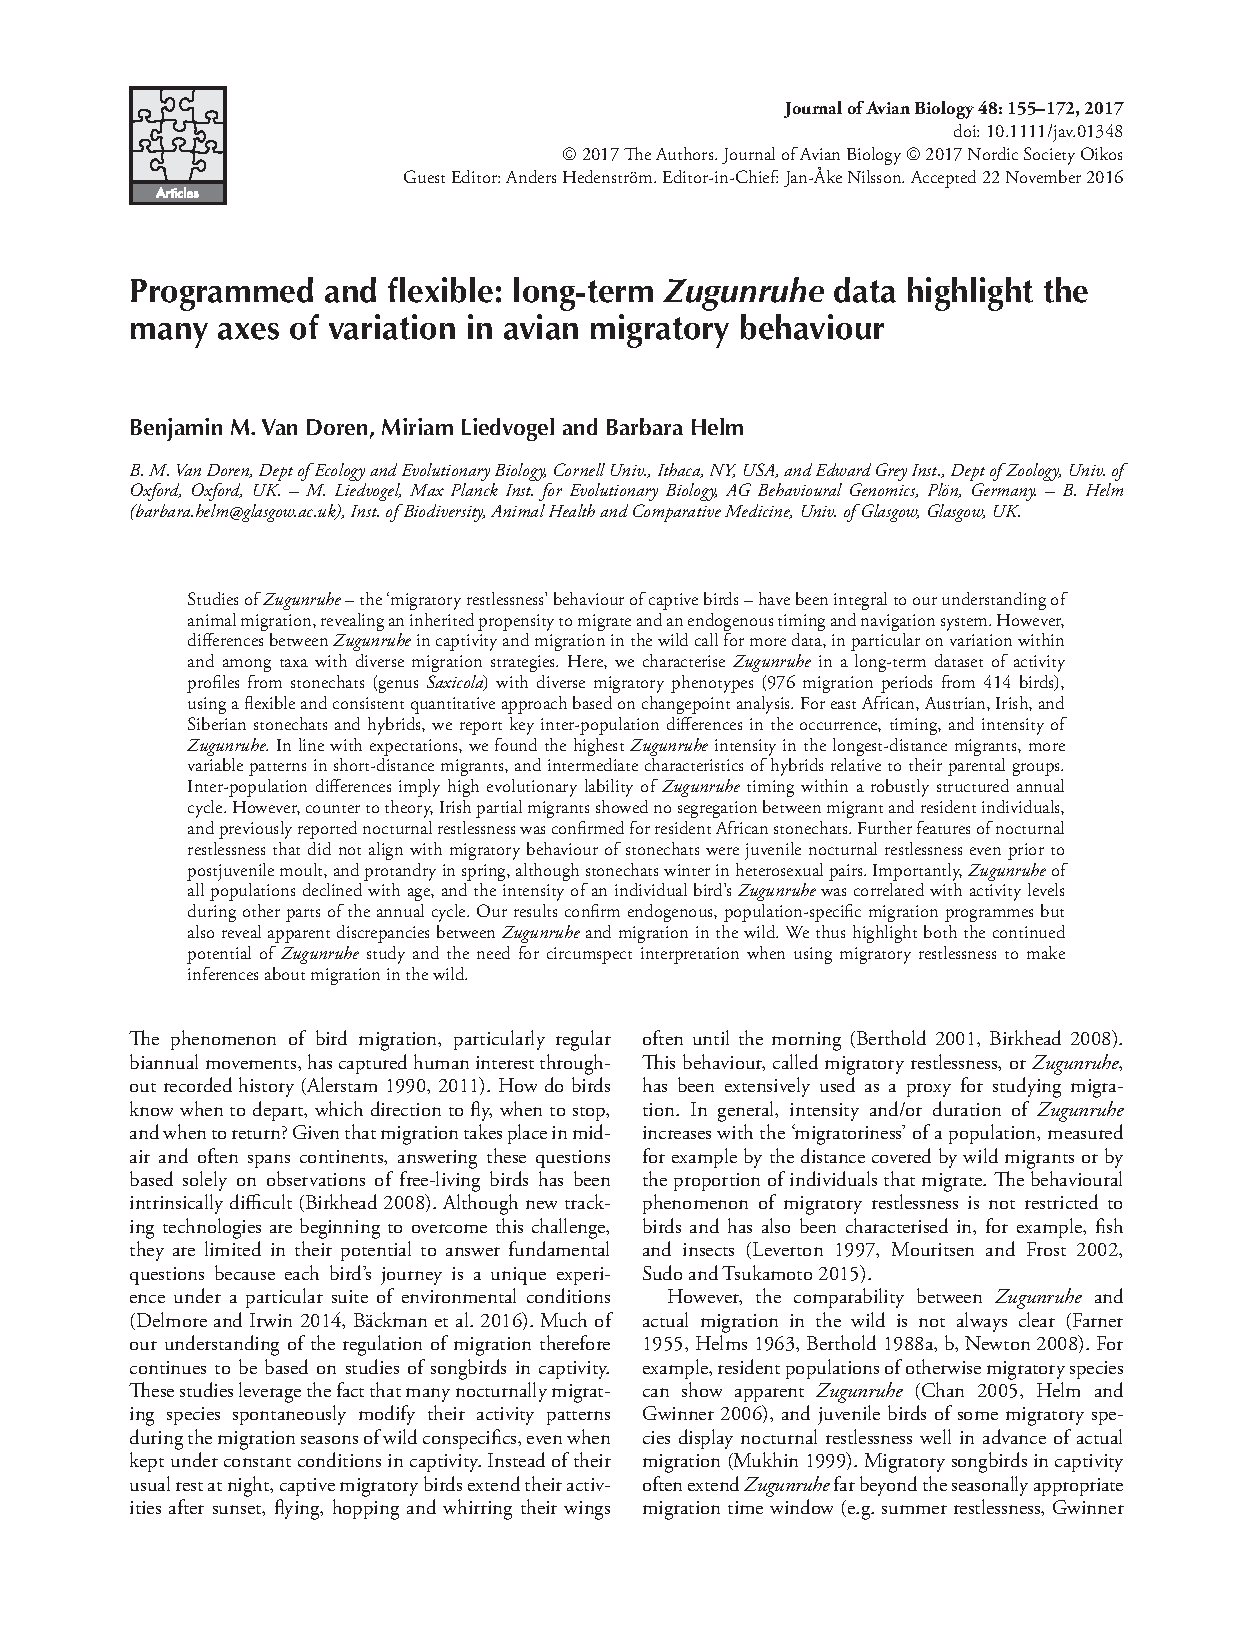
\includegraphics[width=1.15\linewidth]{/Users/Benjamin/Documents/Oxford/Thesis/oxforddown/pdf_chapters/zug/zug_crop_Part01.pdf}} \end{center} \newpage 
 \begin{center} \makebox[\linewidth][c]{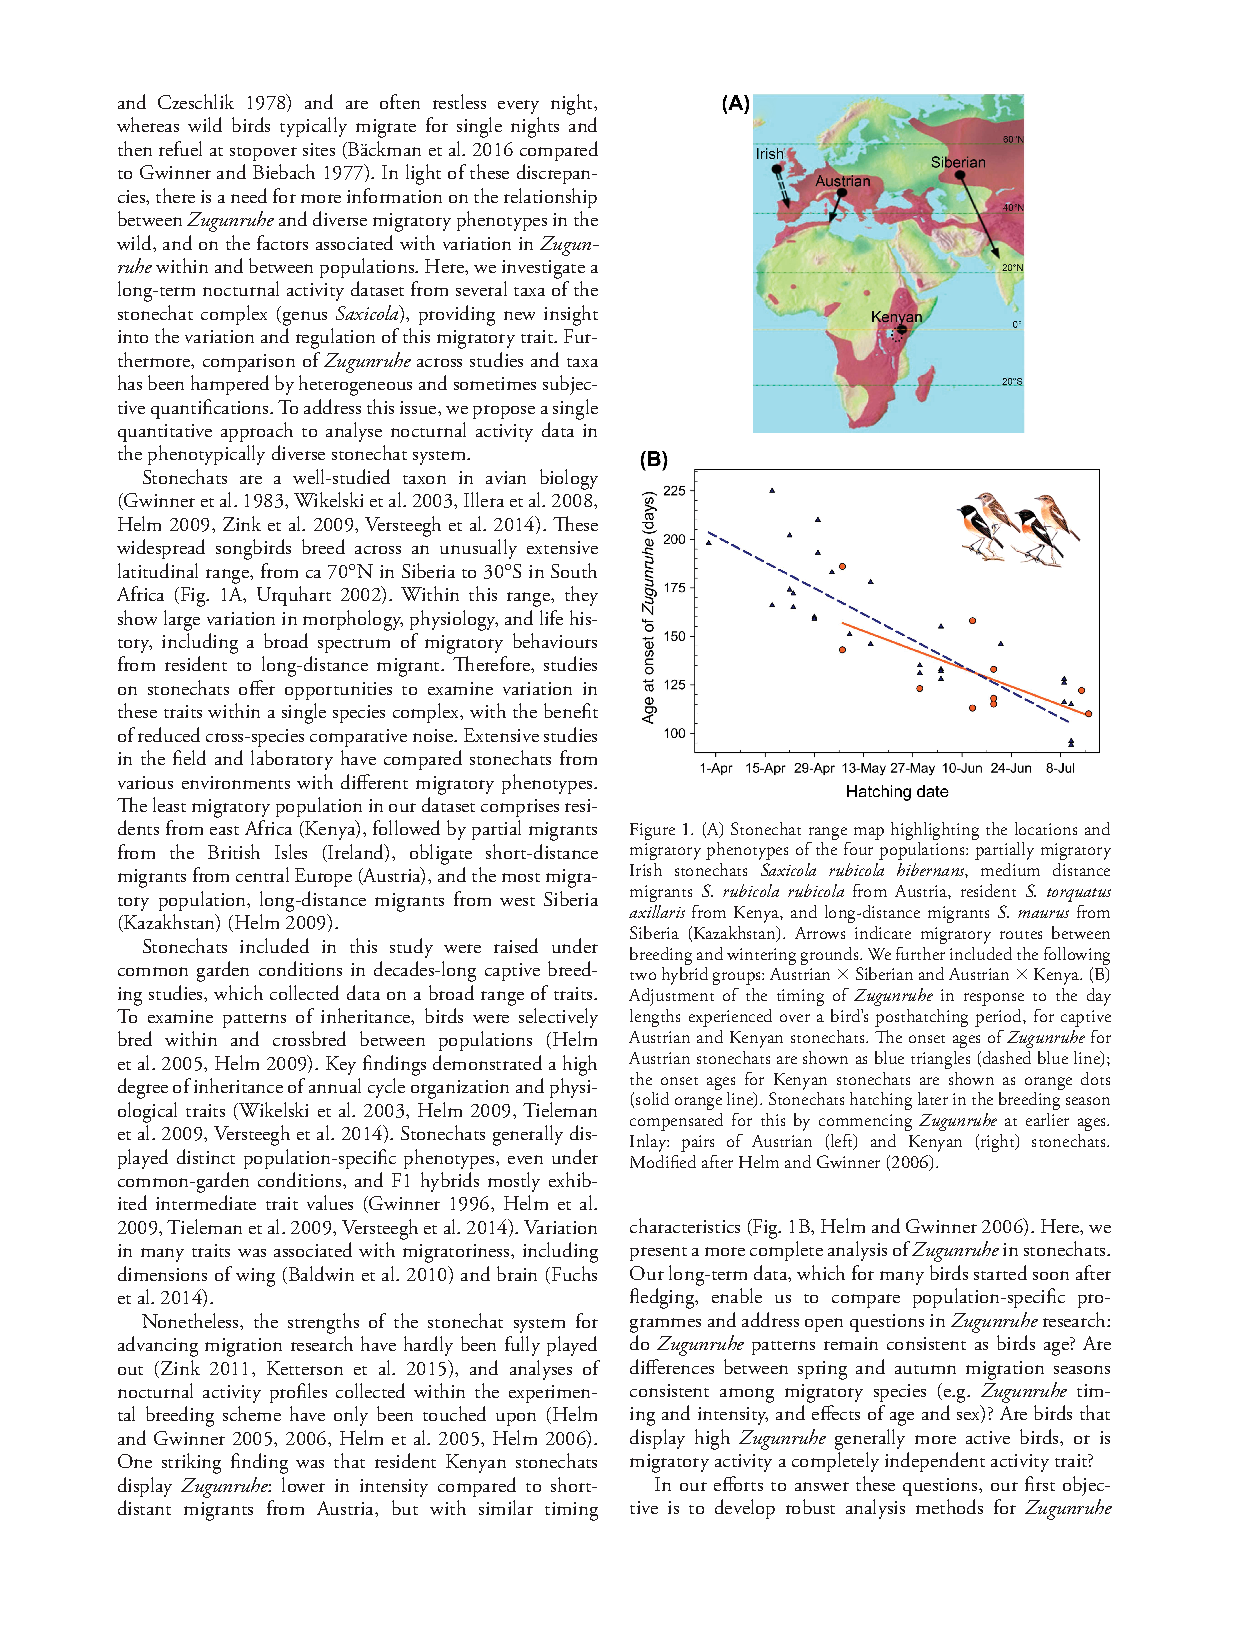
\includegraphics[width=1.15\linewidth]{/Users/Benjamin/Documents/Oxford/Thesis/oxforddown/pdf_chapters/zug/zug_crop_Part02.pdf}} \end{center} \newpage 
 \begin{center} \makebox[\linewidth][c]{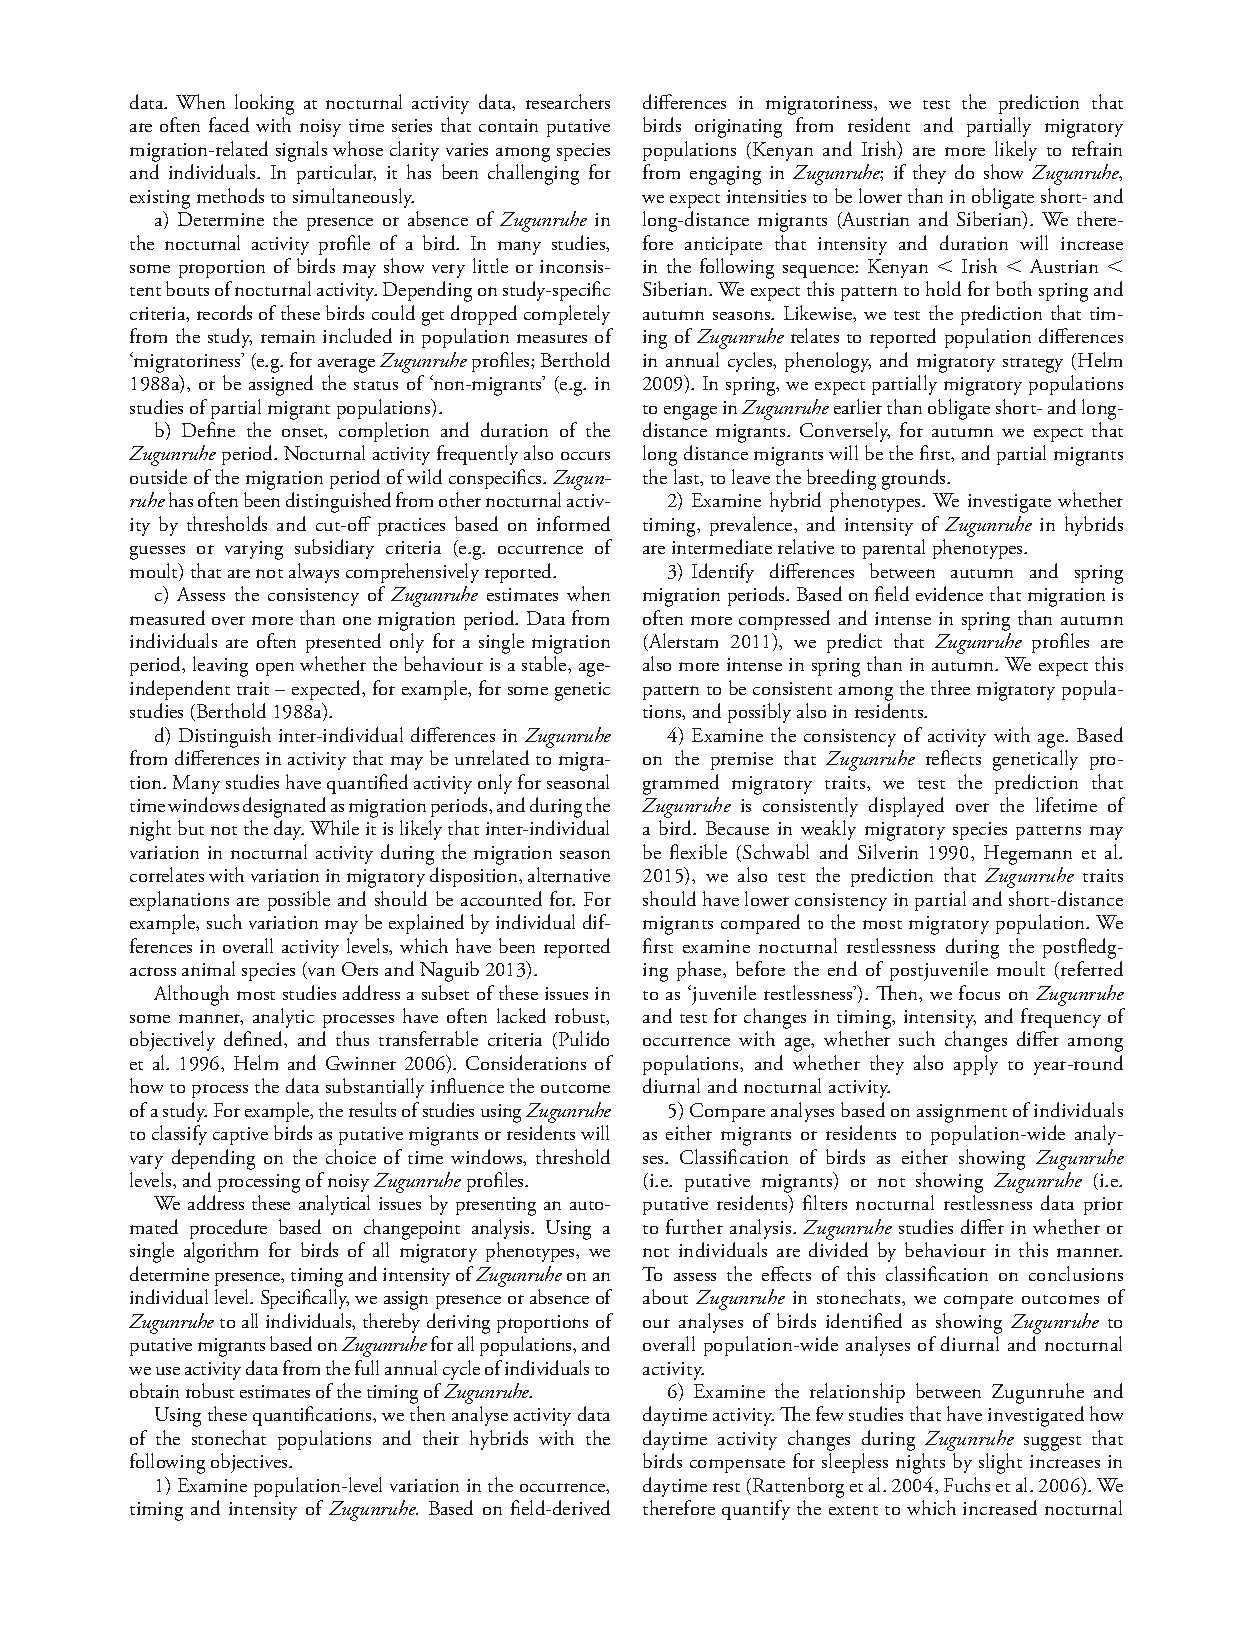
\includegraphics[width=1.15\linewidth]{/Users/Benjamin/Documents/Oxford/Thesis/oxforddown/pdf_chapters/zug/zug_crop_Part03.pdf}} \end{center} \newpage 
 \begin{center} \makebox[\linewidth][c]{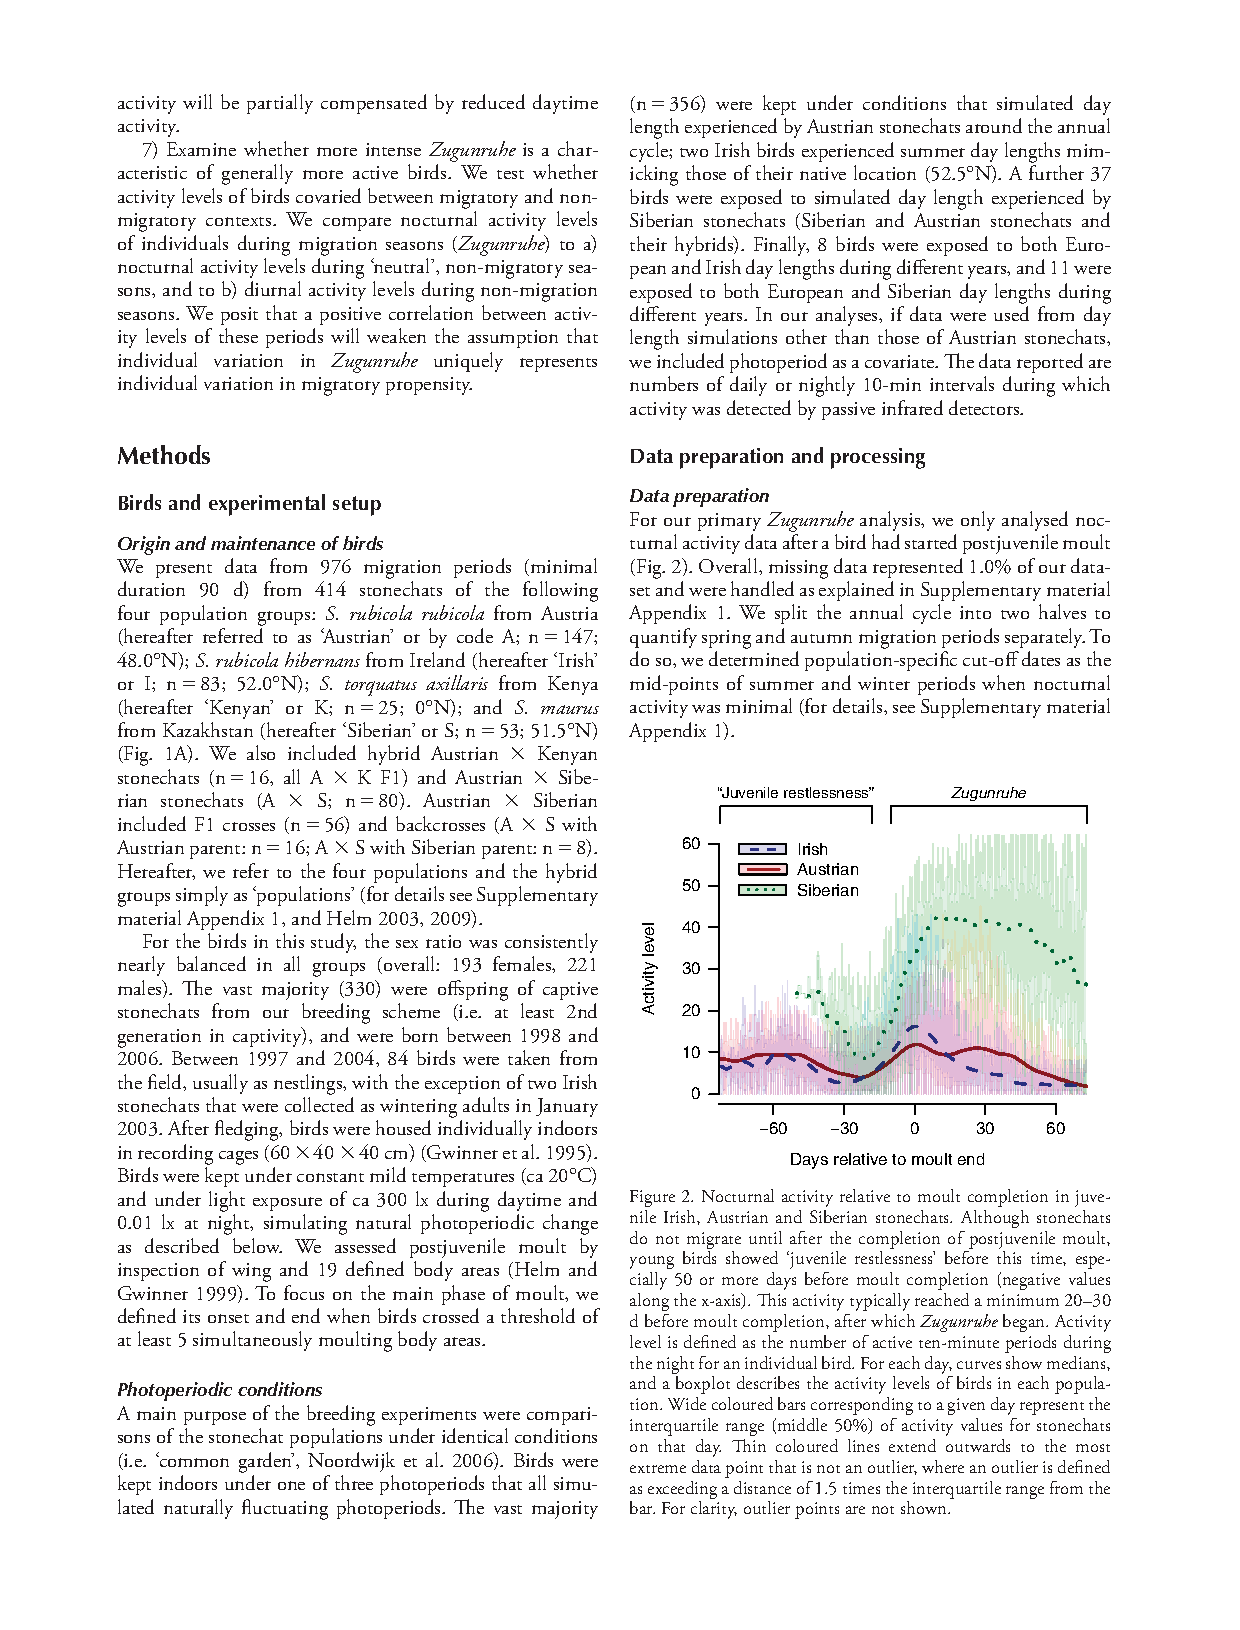
\includegraphics[width=1.15\linewidth]{/Users/Benjamin/Documents/Oxford/Thesis/oxforddown/pdf_chapters/zug/zug_crop_Part04.pdf}} \end{center} \newpage 
 \begin{center} \makebox[\linewidth][c]{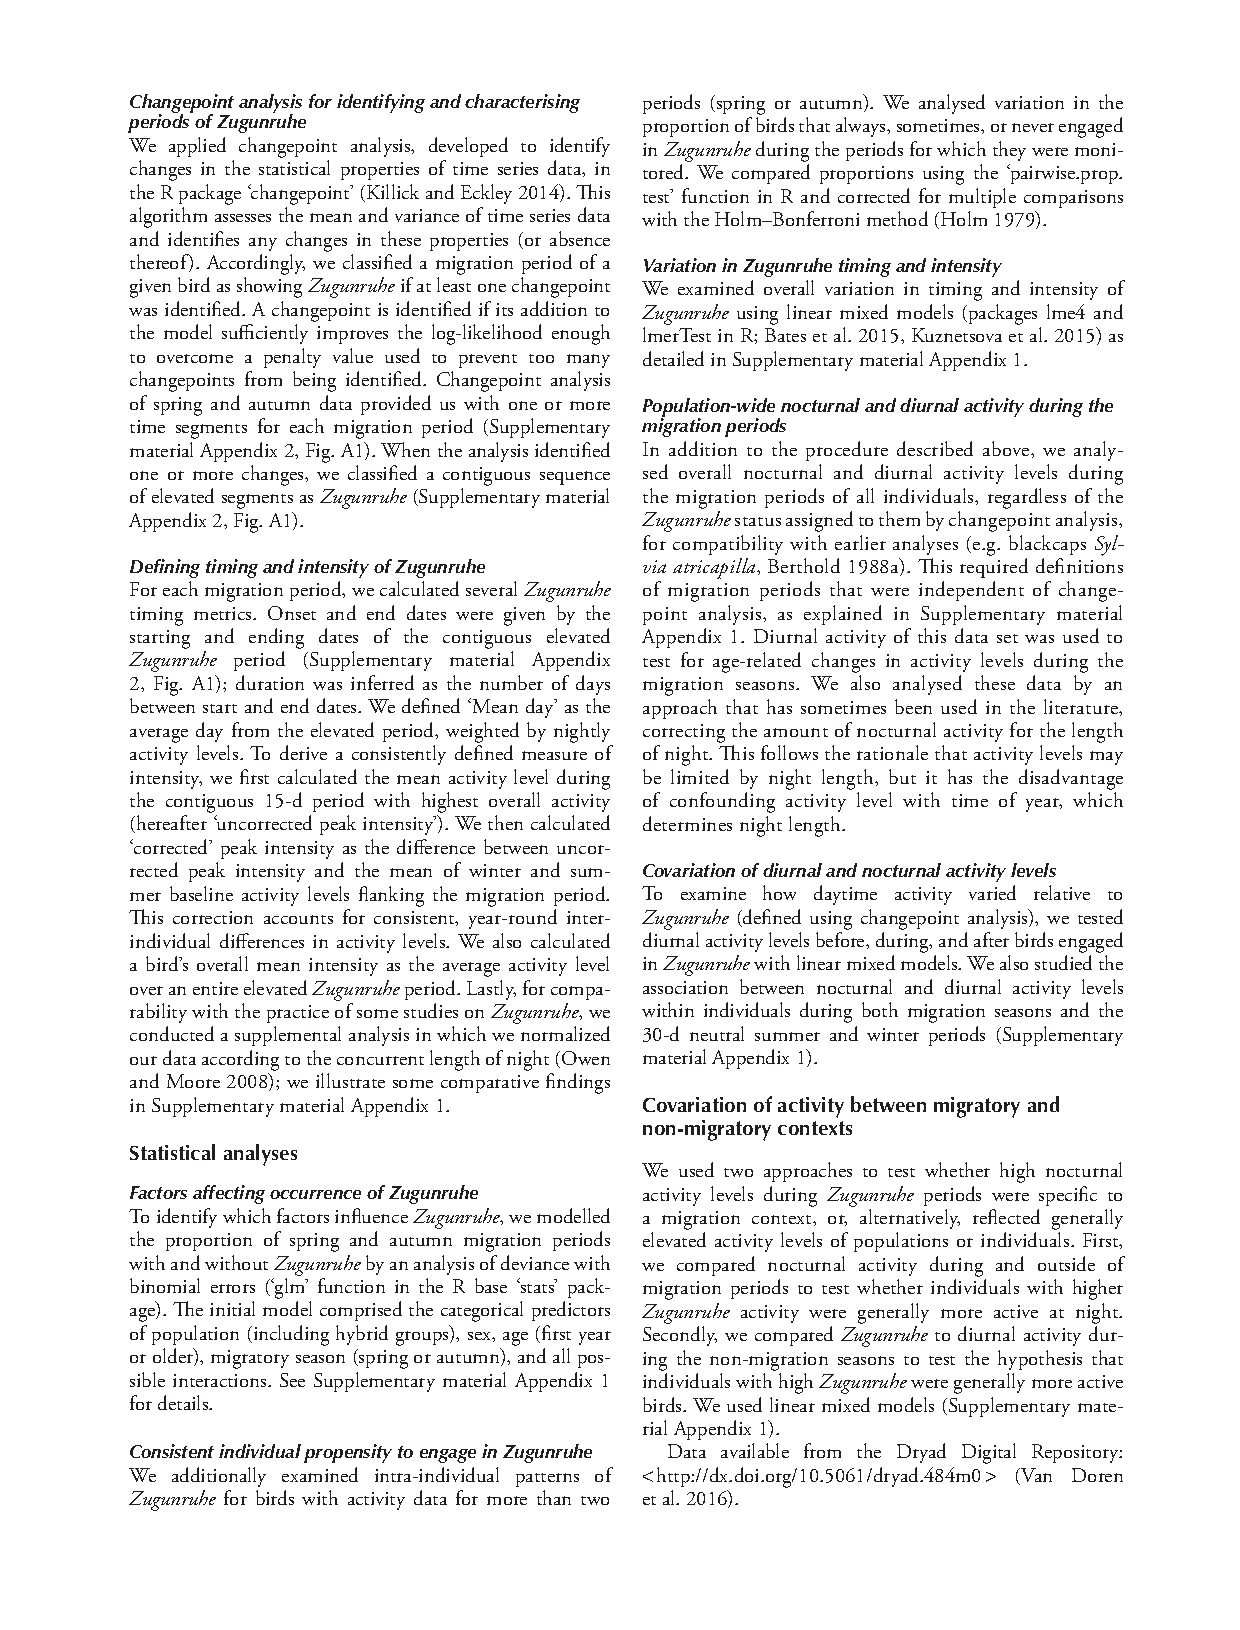
\includegraphics[width=1.15\linewidth]{/Users/Benjamin/Documents/Oxford/Thesis/oxforddown/pdf_chapters/zug/zug_crop_Part05.pdf}} \end{center} \newpage 
 \begin{center} \makebox[\linewidth][c]{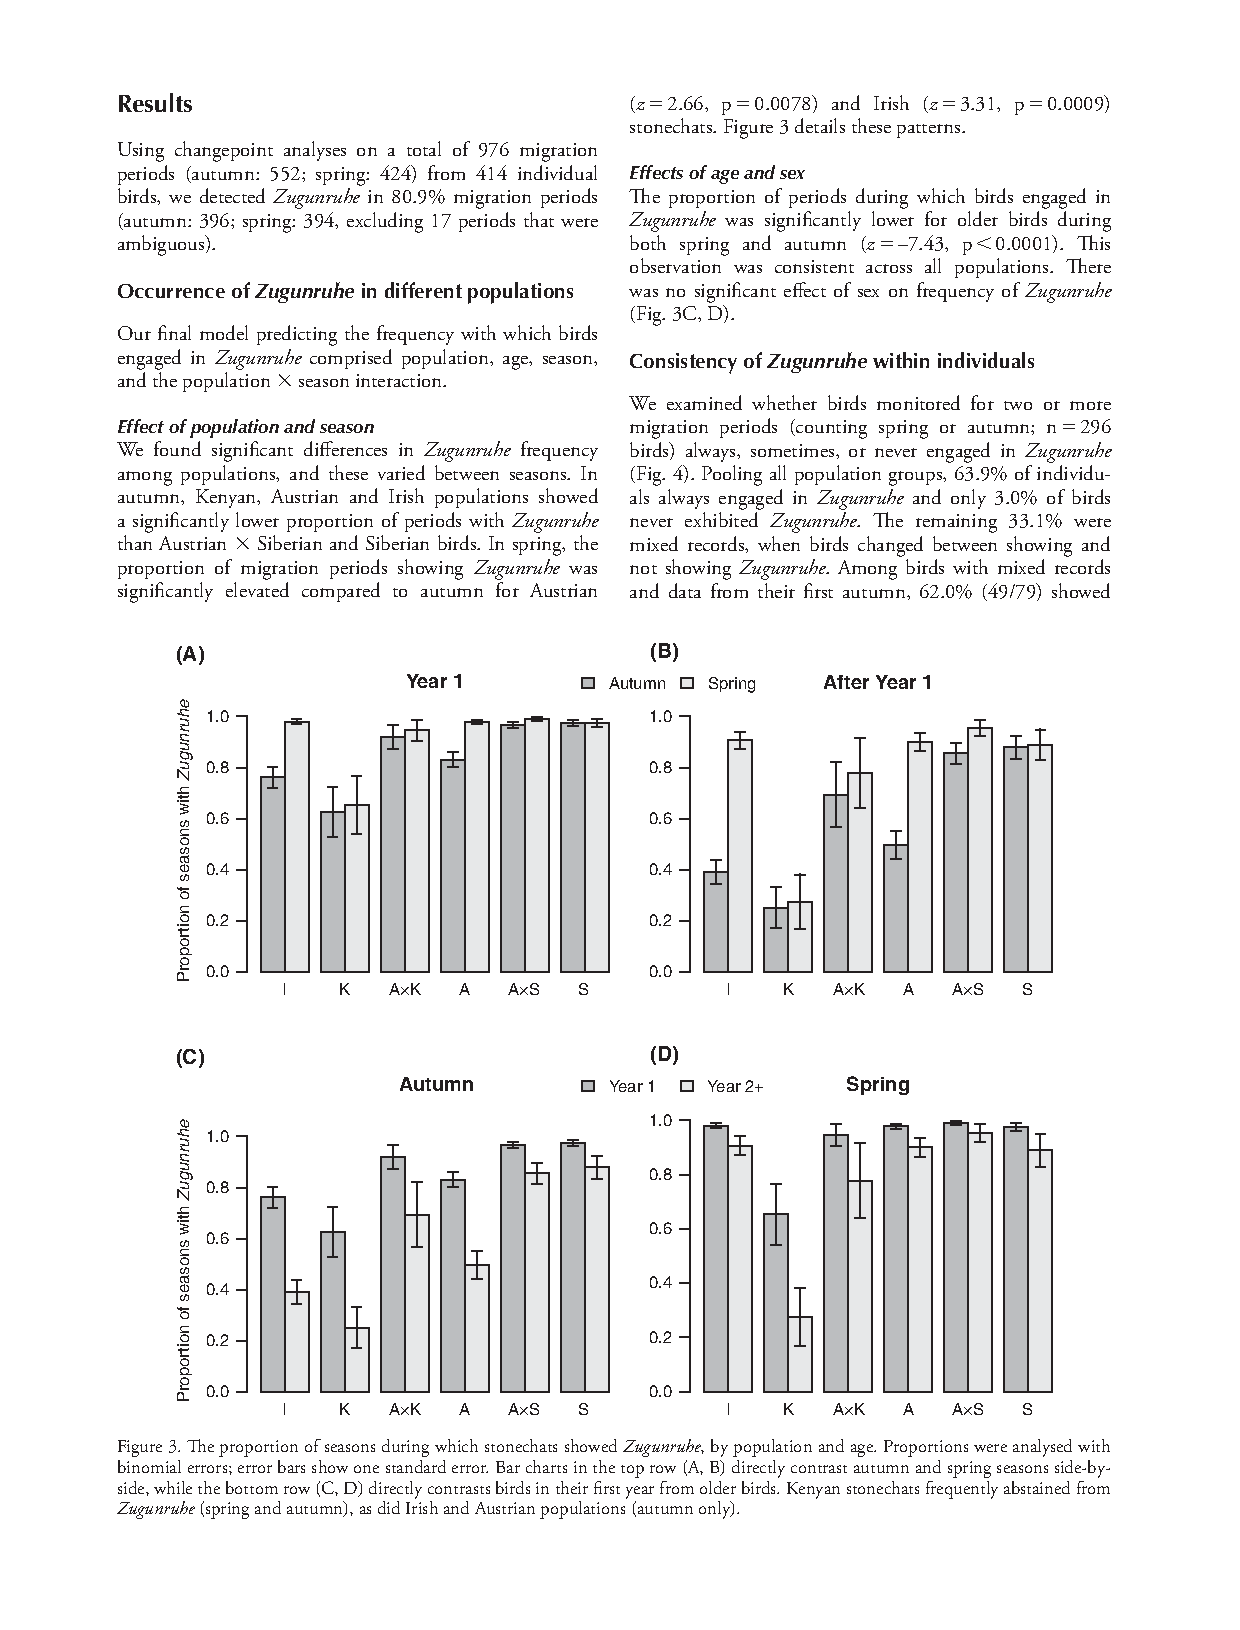
\includegraphics[width=1.15\linewidth]{/Users/Benjamin/Documents/Oxford/Thesis/oxforddown/pdf_chapters/zug/zug_crop_Part06.pdf}} \end{center} \newpage 
 \begin{center} \makebox[\linewidth][c]{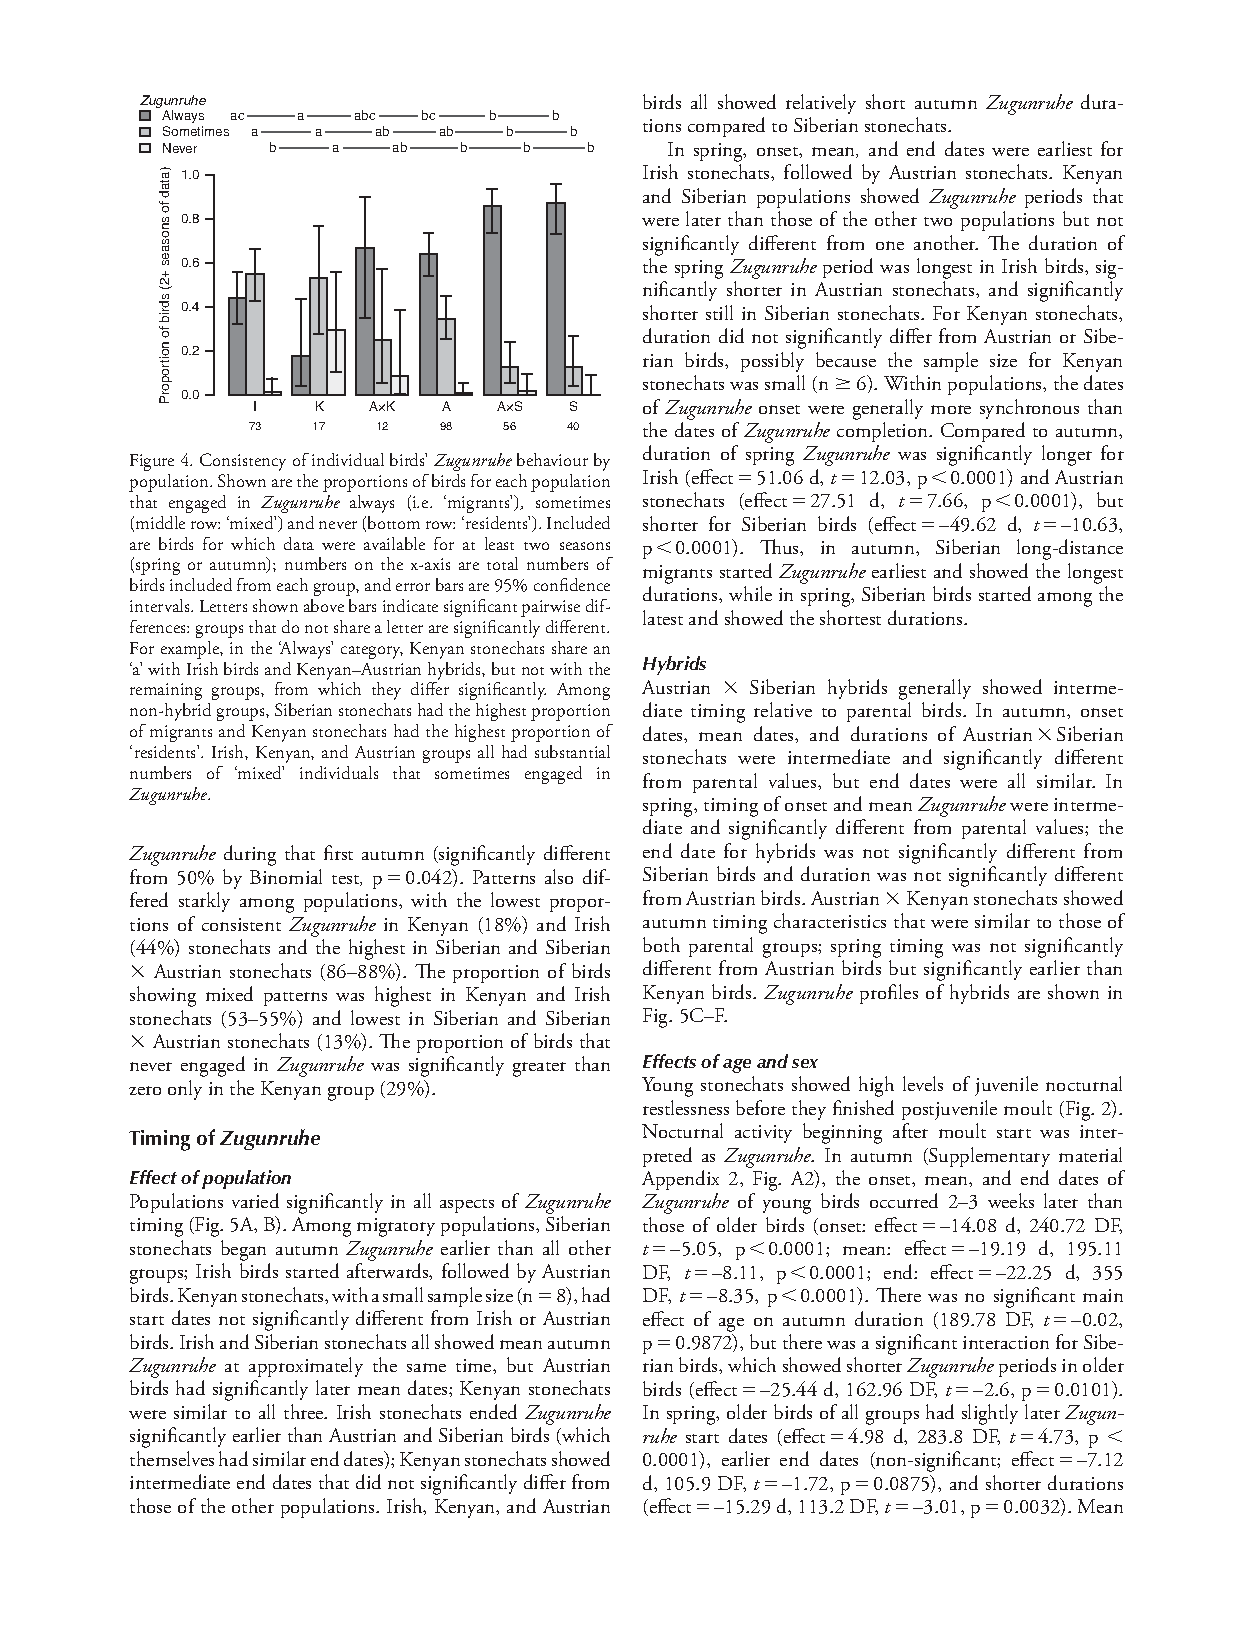
\includegraphics[width=1.15\linewidth]{/Users/Benjamin/Documents/Oxford/Thesis/oxforddown/pdf_chapters/zug/zug_crop_Part07.pdf}} \end{center} \newpage 
 \begin{center} \makebox[\linewidth][c]{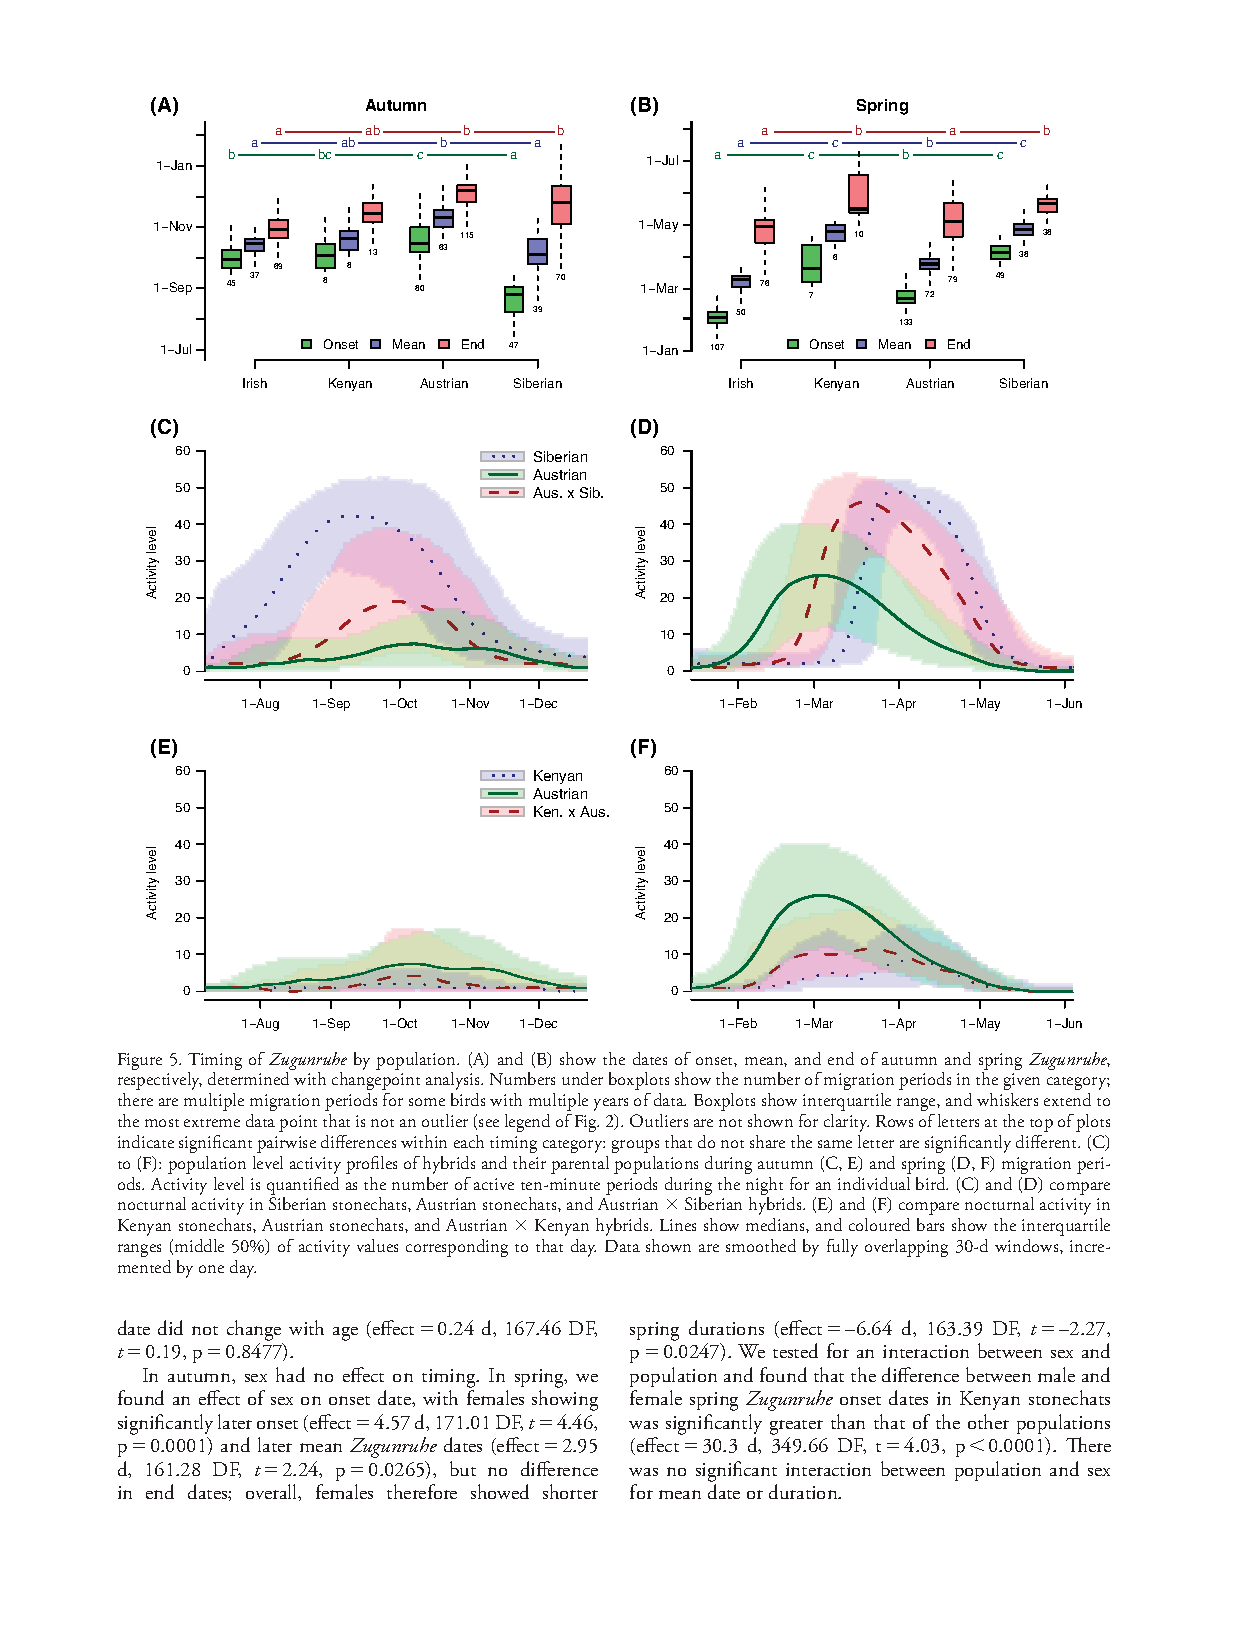
\includegraphics[width=1.15\linewidth]{/Users/Benjamin/Documents/Oxford/Thesis/oxforddown/pdf_chapters/zug/zug_crop_Part08.pdf}} \end{center} \newpage 
 \begin{center} \makebox[\linewidth][c]{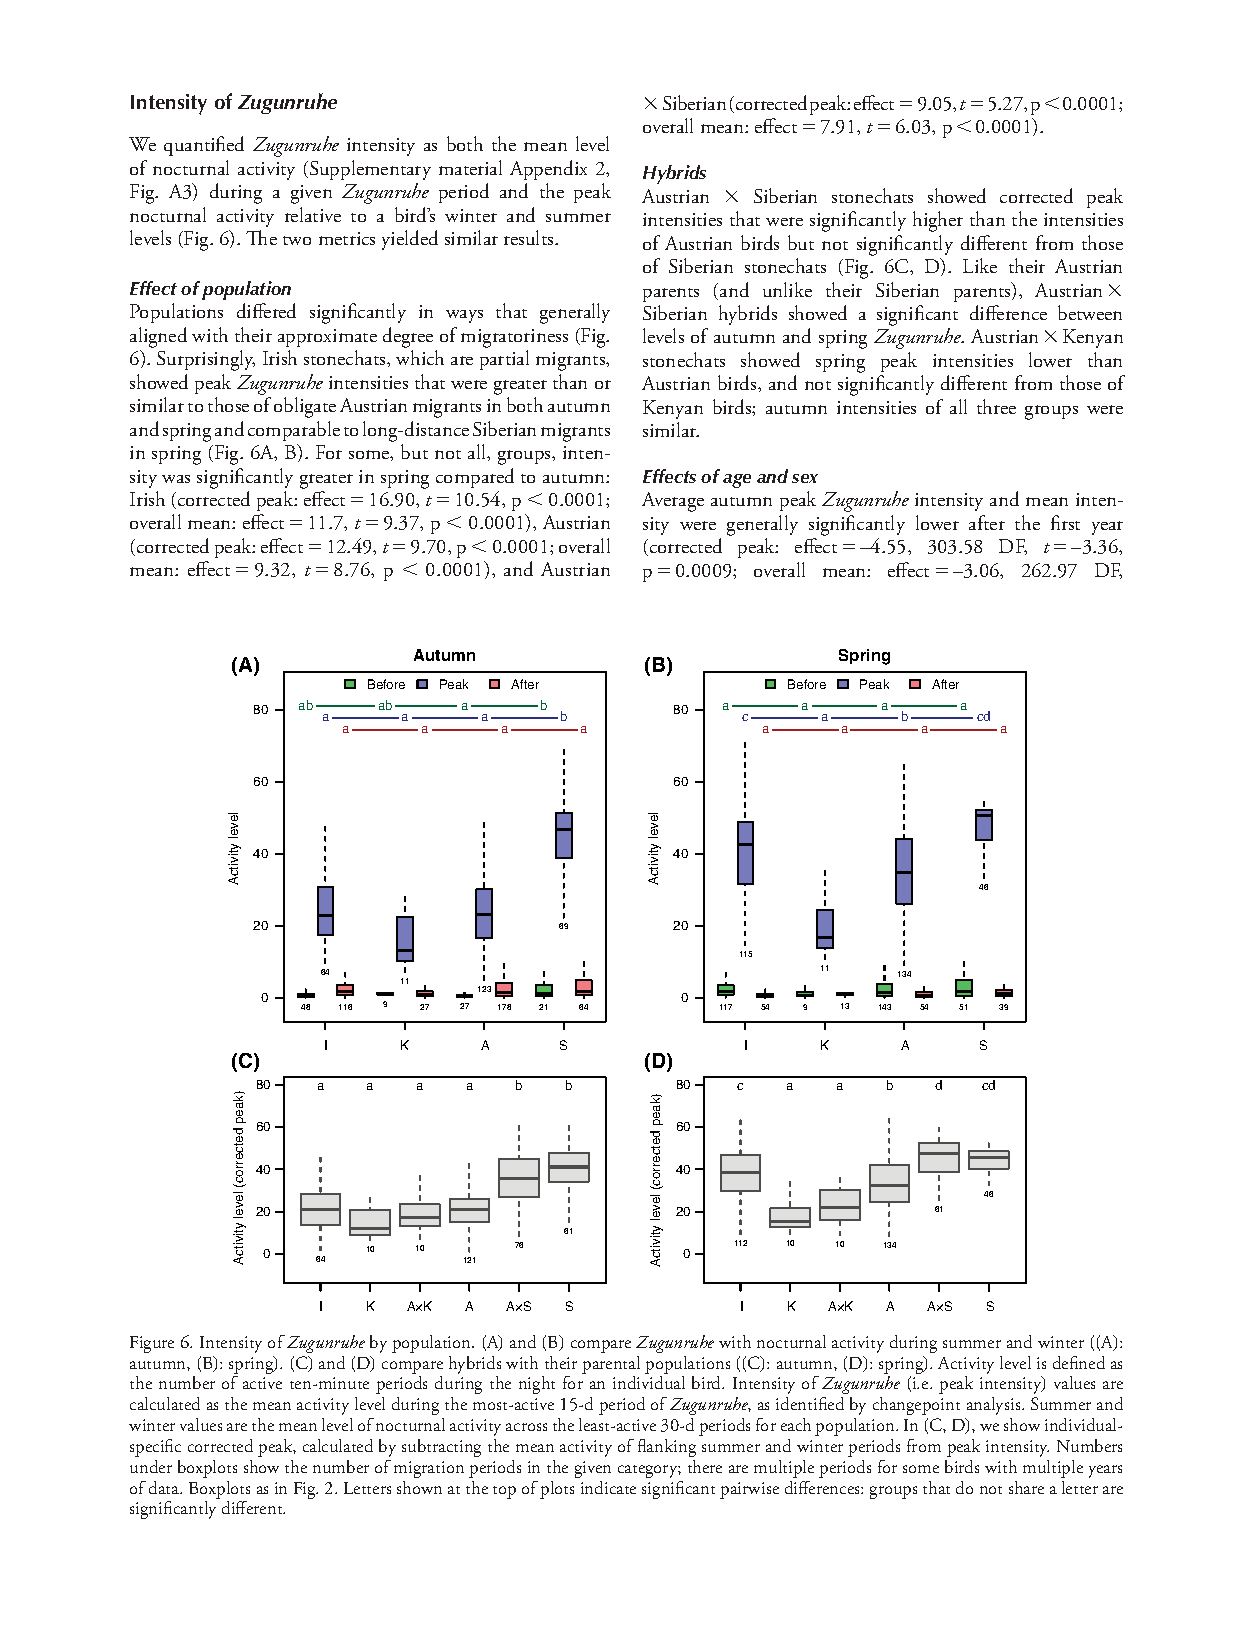
\includegraphics[width=1.15\linewidth]{/Users/Benjamin/Documents/Oxford/Thesis/oxforddown/pdf_chapters/zug/zug_crop_Part09.pdf}} \end{center} \newpage 
 \begin{center} \makebox[\linewidth][c]{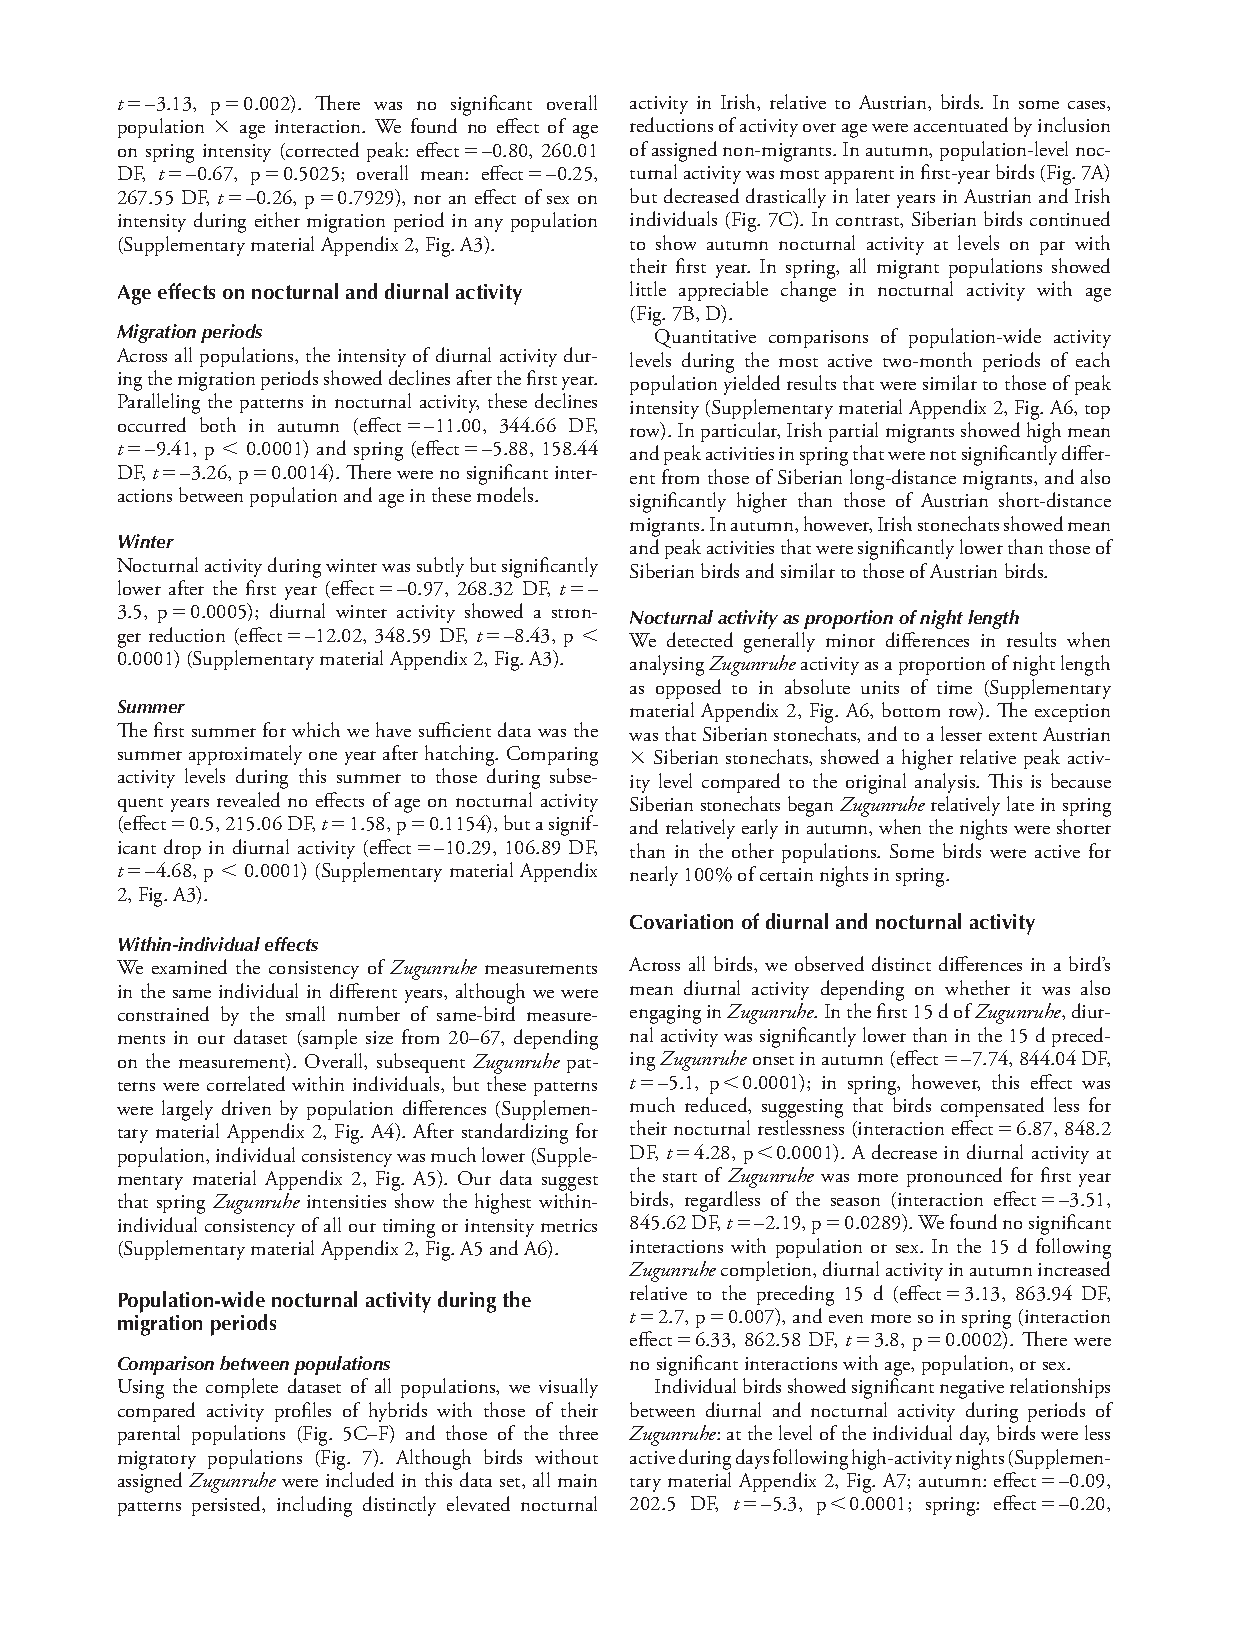
\includegraphics[width=1.15\linewidth]{/Users/Benjamin/Documents/Oxford/Thesis/oxforddown/pdf_chapters/zug/zug_crop_Part10.pdf}} \end{center} \newpage 
 \begin{center} \makebox[\linewidth][c]{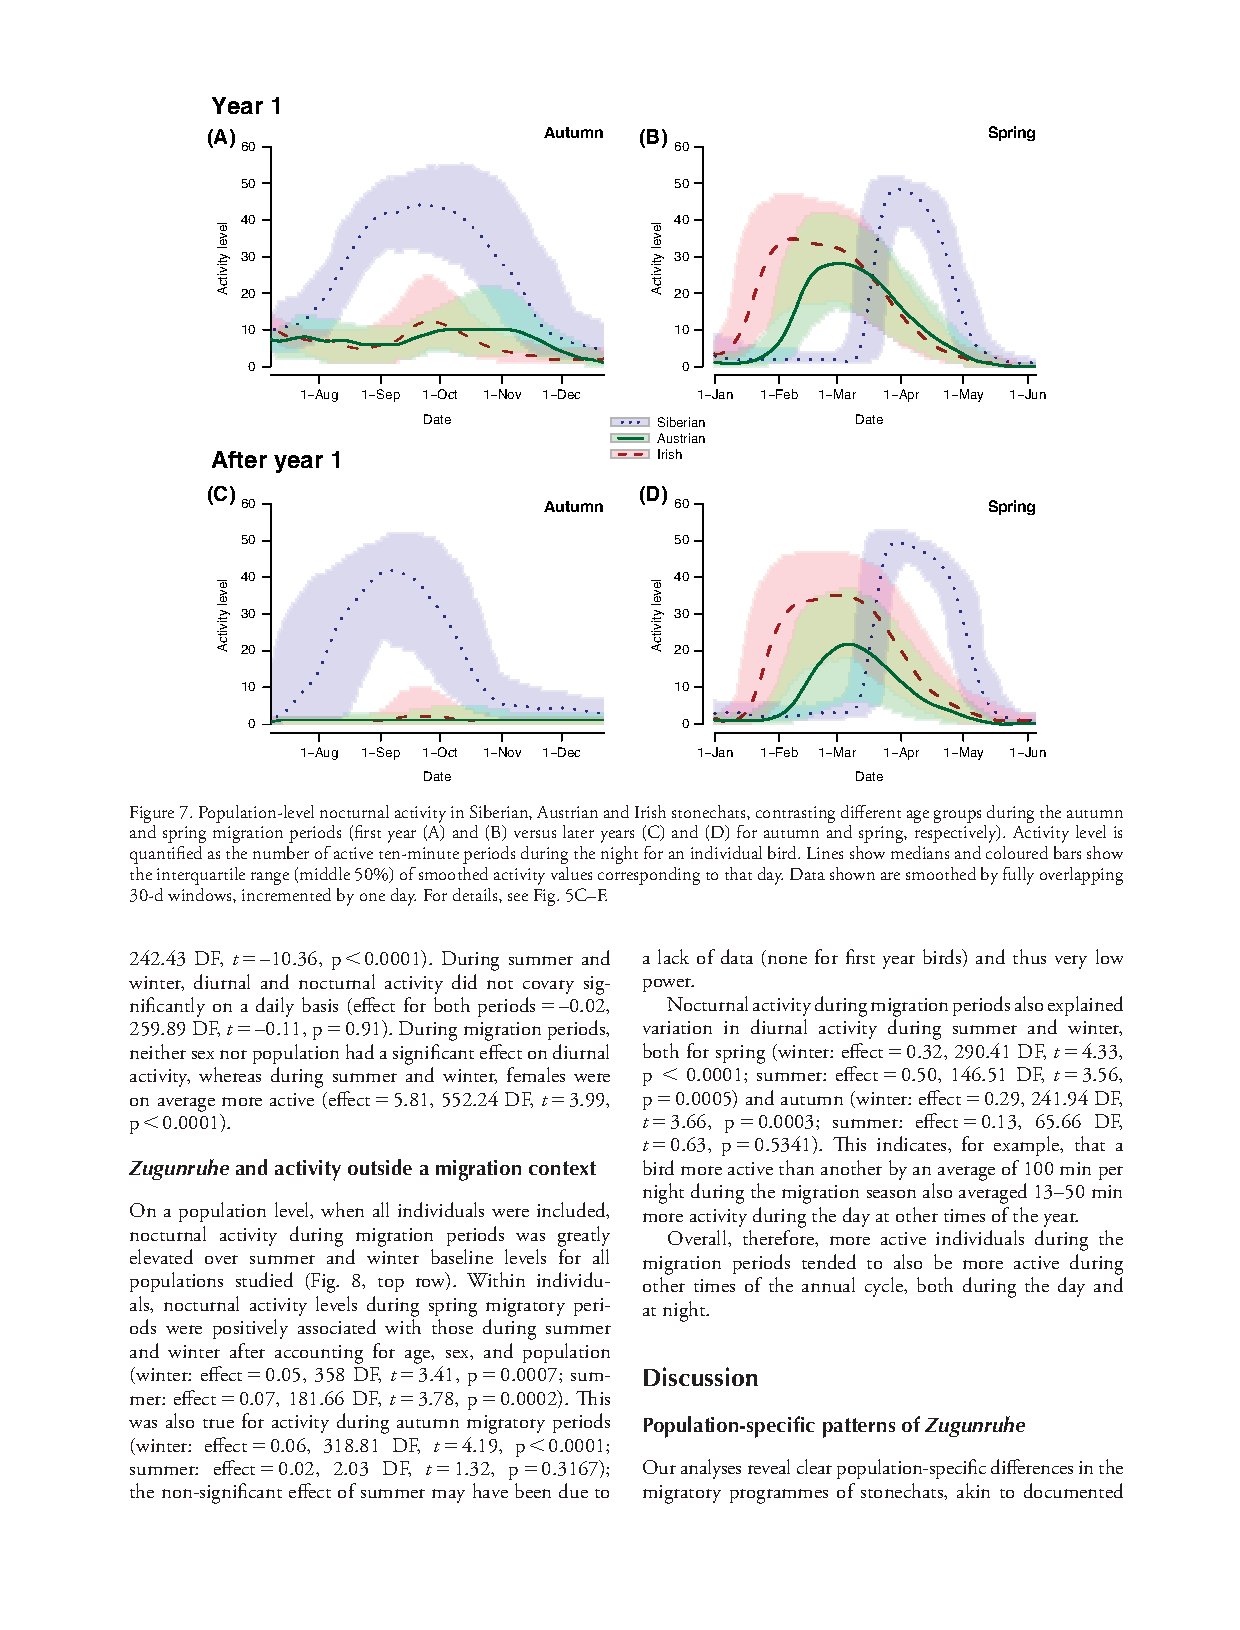
\includegraphics[width=1.15\linewidth]{/Users/Benjamin/Documents/Oxford/Thesis/oxforddown/pdf_chapters/zug/zug_crop_Part11.pdf}} \end{center} \newpage 
 \begin{center} \makebox[\linewidth][c]{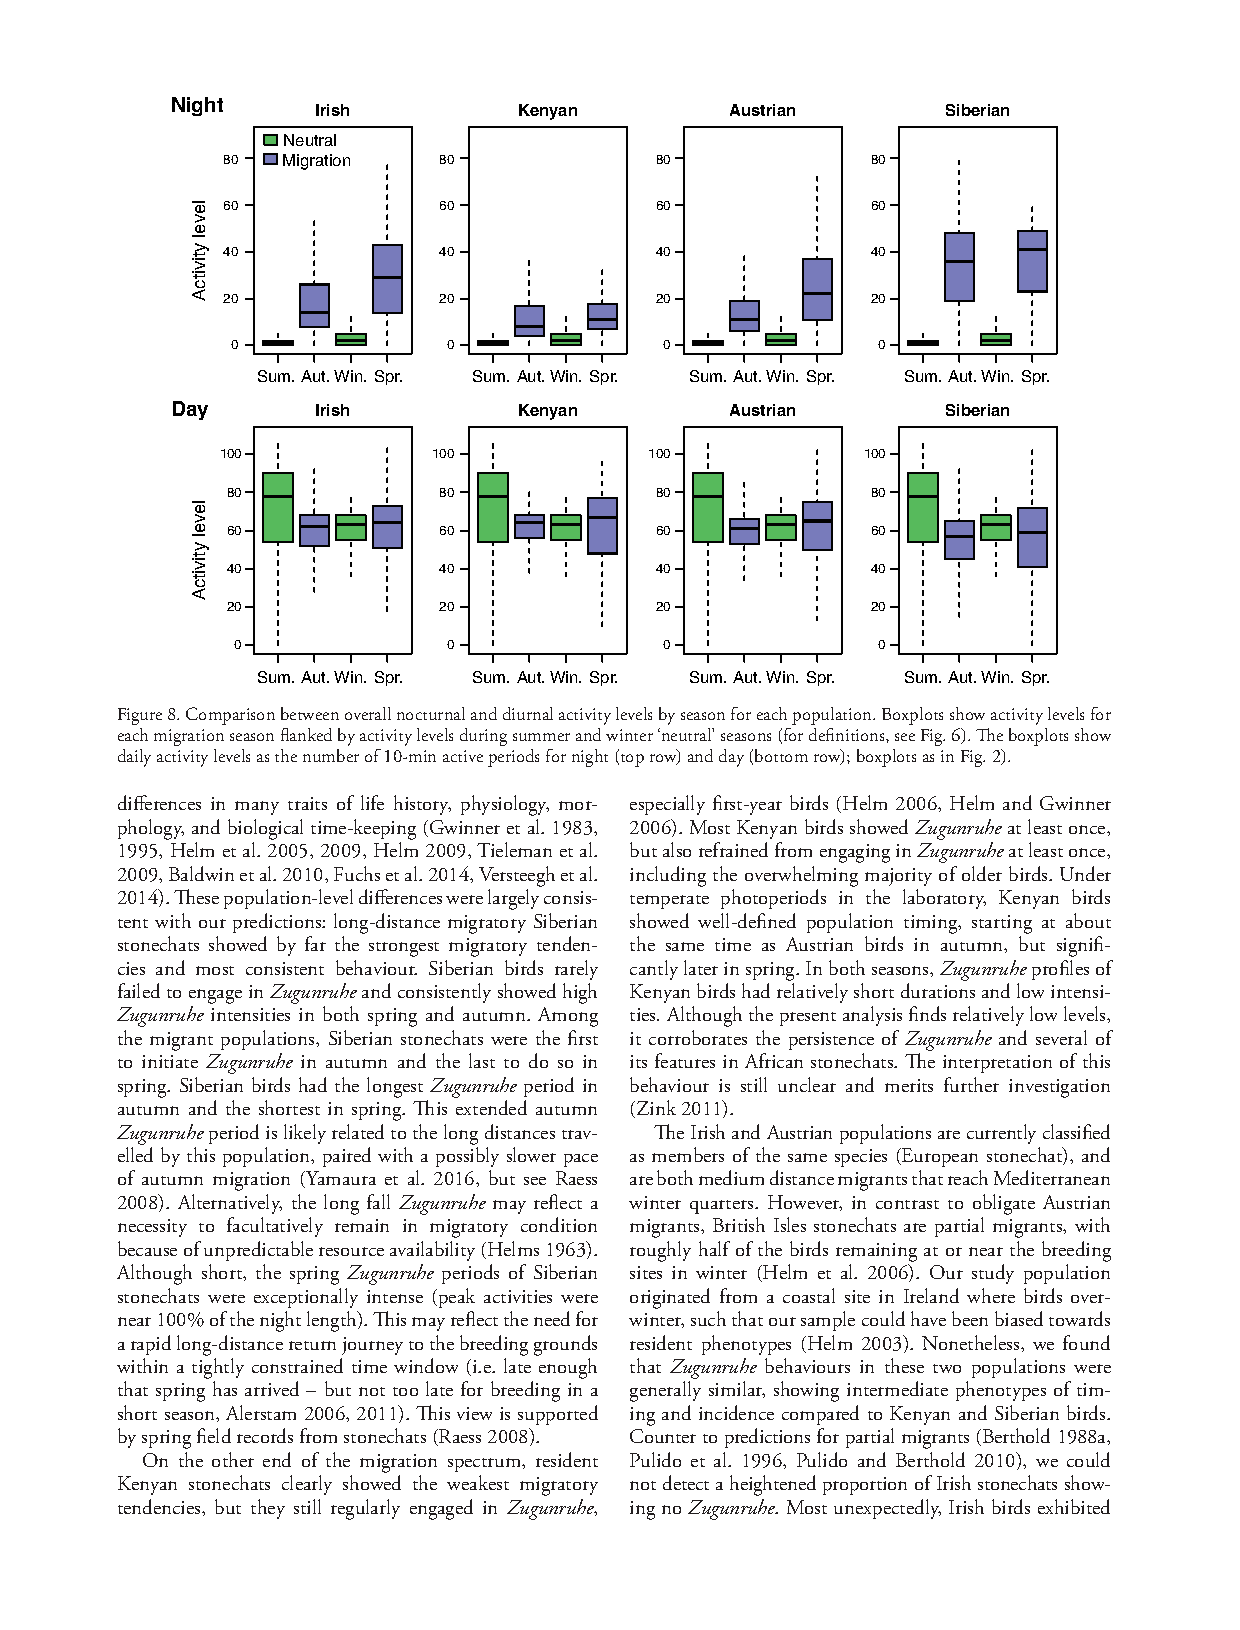
\includegraphics[width=1.15\linewidth]{/Users/Benjamin/Documents/Oxford/Thesis/oxforddown/pdf_chapters/zug/zug_crop_Part12.pdf}} \end{center} \newpage 
 \begin{center} \makebox[\linewidth][c]{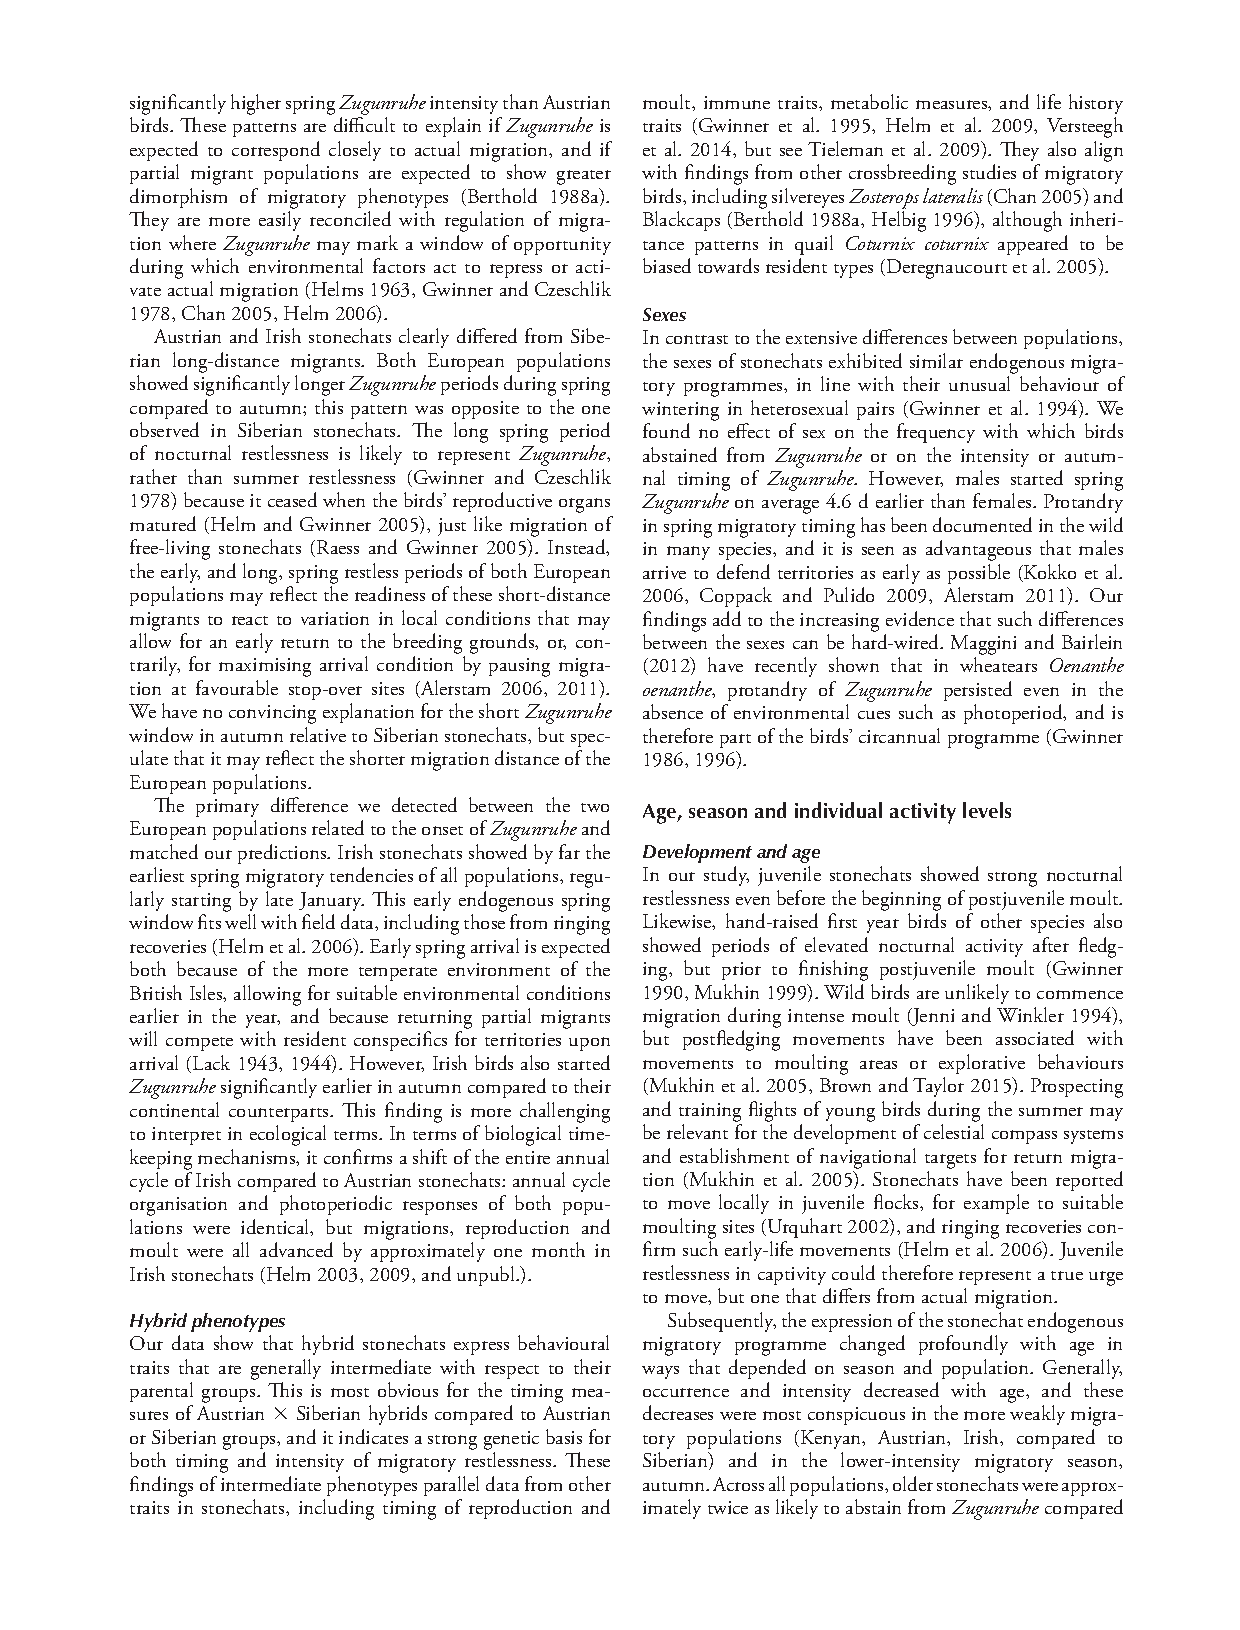
\includegraphics[width=1.15\linewidth]{/Users/Benjamin/Documents/Oxford/Thesis/oxforddown/pdf_chapters/zug/zug_crop_Part13.pdf}} \end{center} \newpage 
 \begin{center} \makebox[\linewidth][c]{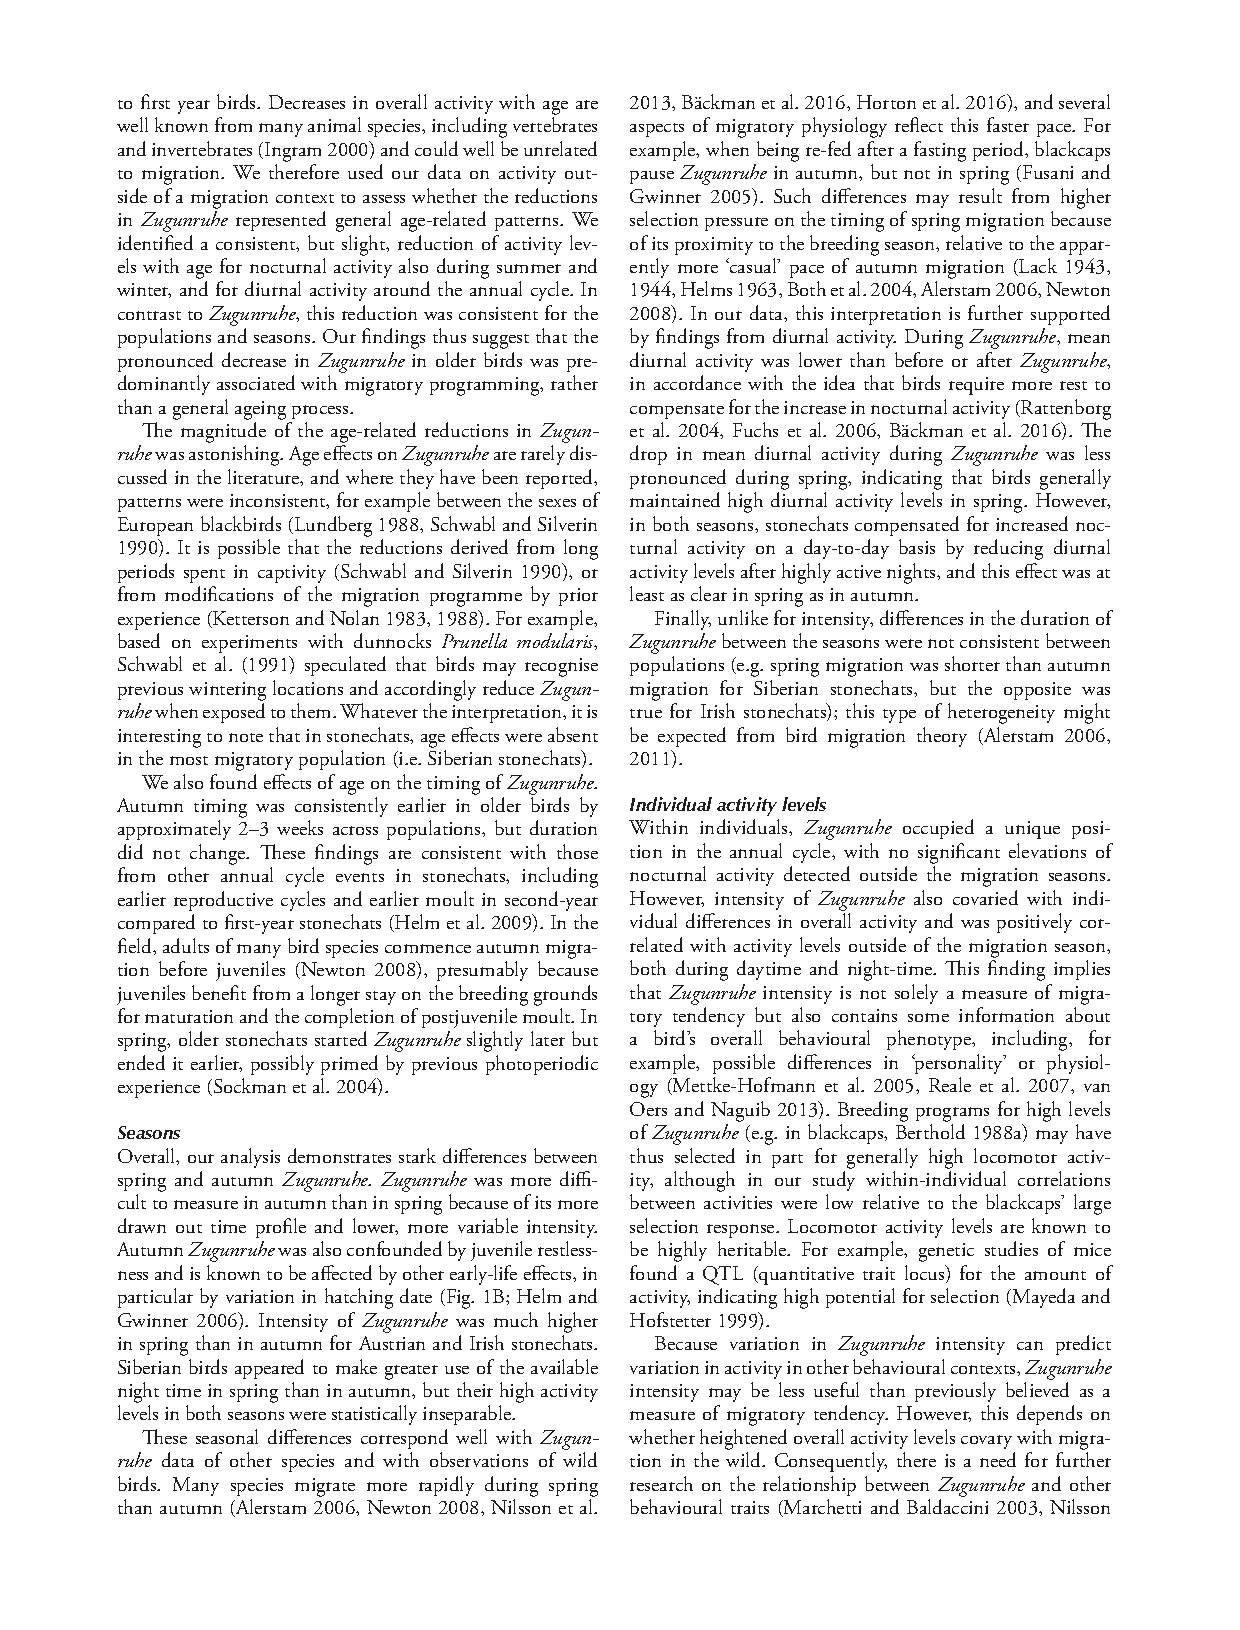
\includegraphics[width=1.15\linewidth]{/Users/Benjamin/Documents/Oxford/Thesis/oxforddown/pdf_chapters/zug/zug_crop_Part14.pdf}} \end{center} \newpage 
 \begin{center} \makebox[\linewidth][c]{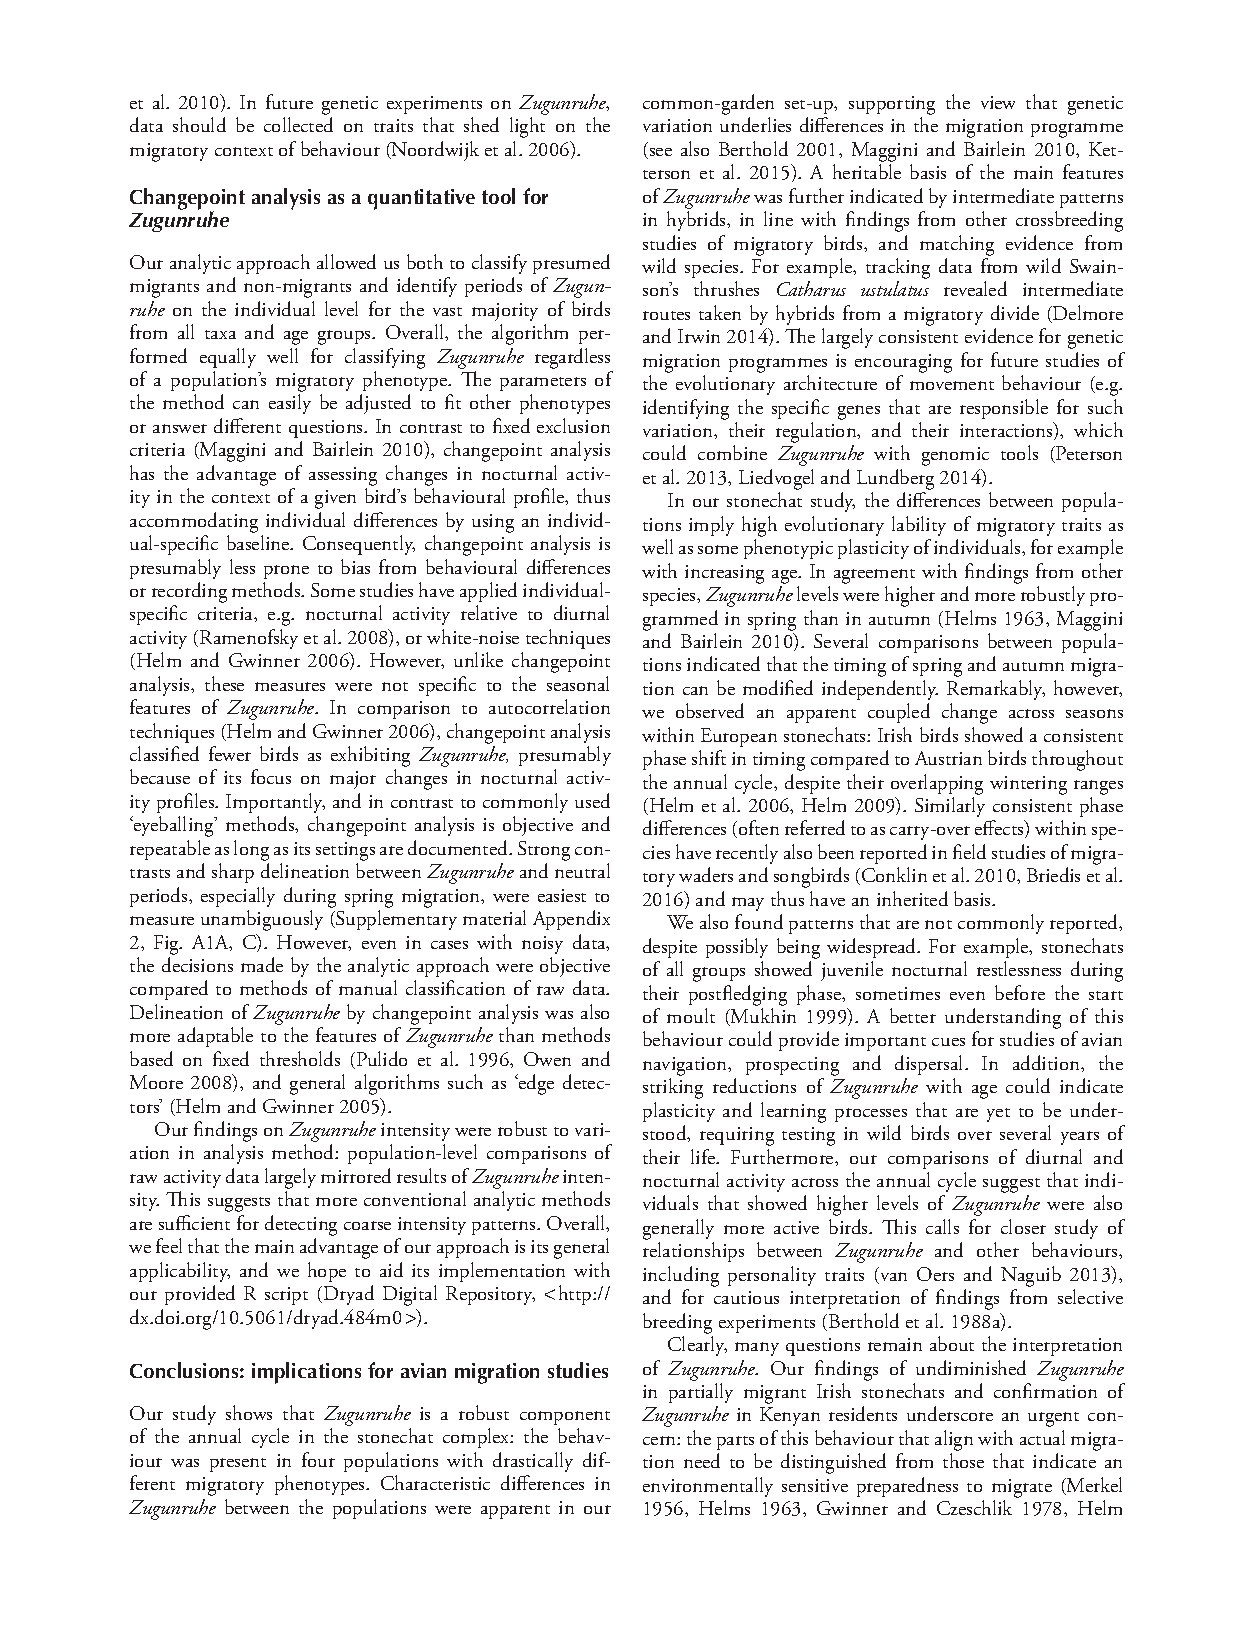
\includegraphics[width=1.15\linewidth]{/Users/Benjamin/Documents/Oxford/Thesis/oxforddown/pdf_chapters/zug/zug_crop_Part15.pdf}} \end{center} \newpage 
 \begin{center} \makebox[\linewidth][c]{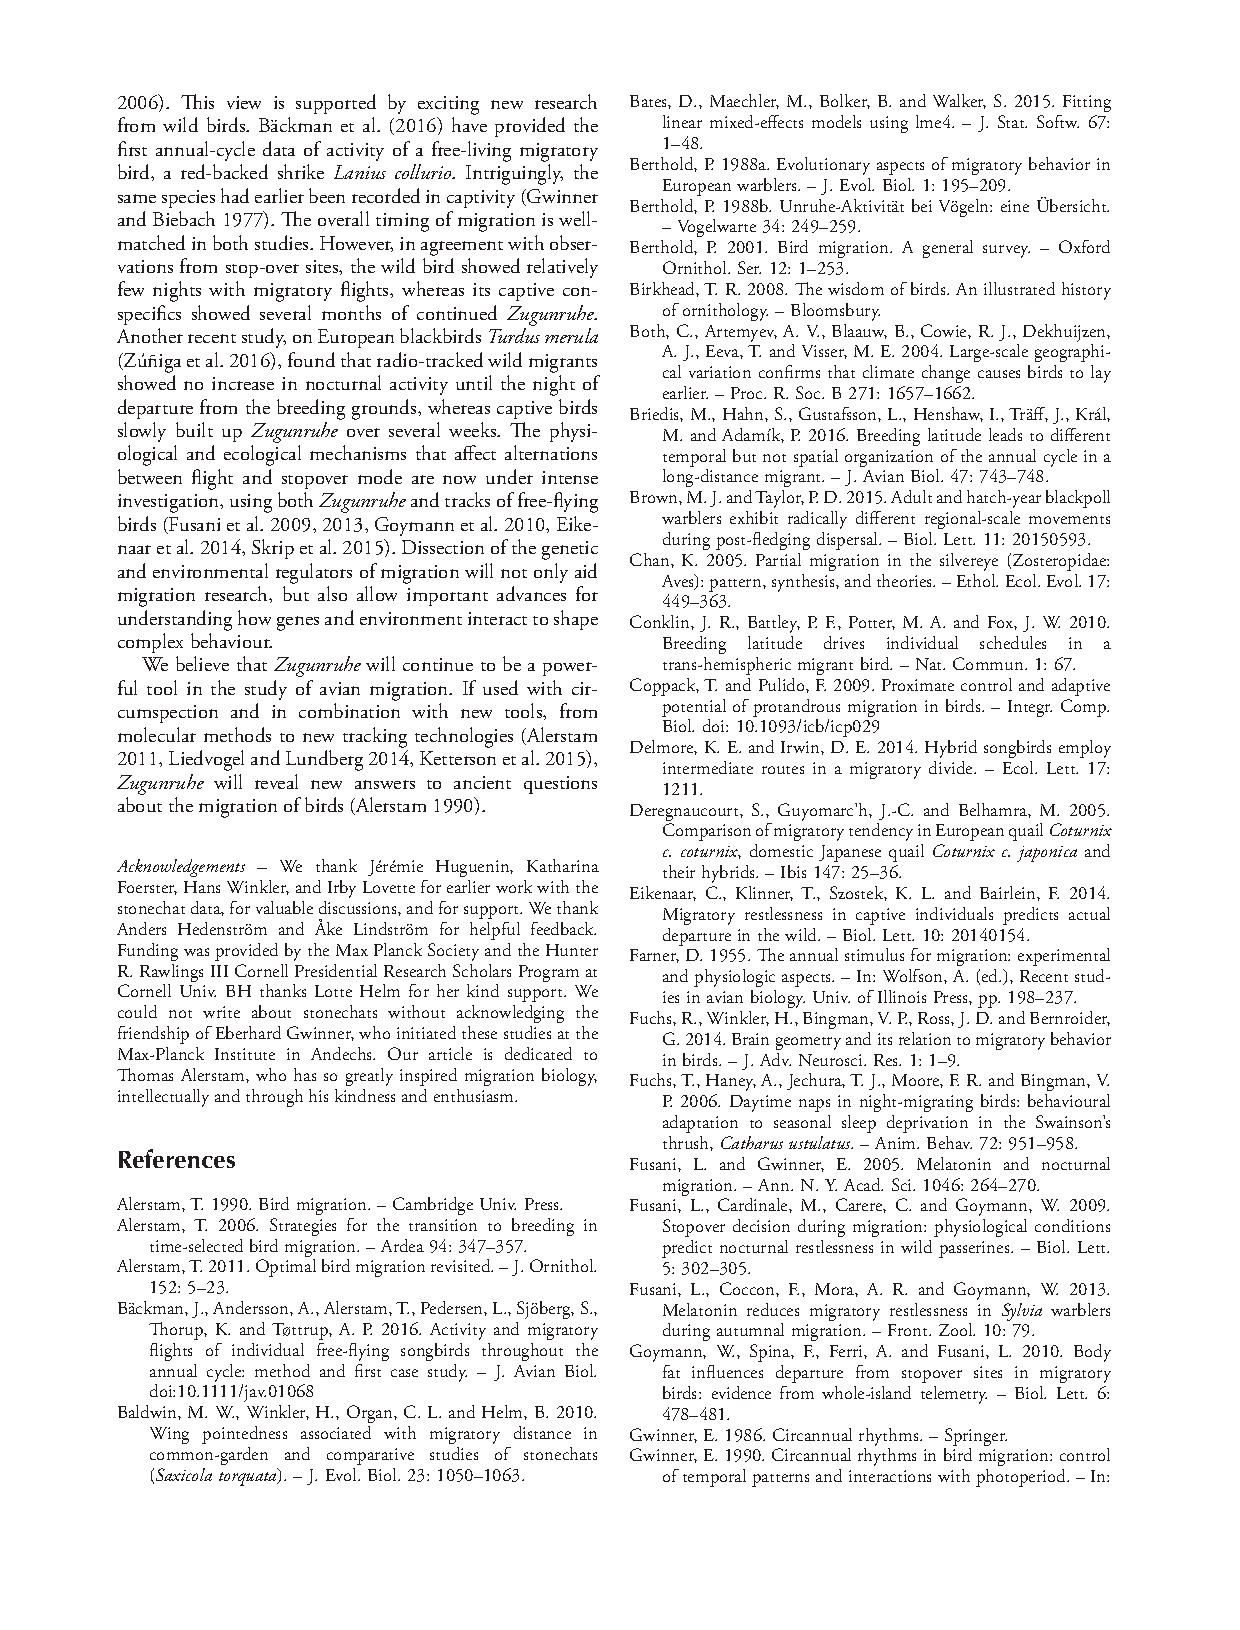
\includegraphics[width=1.15\linewidth]{/Users/Benjamin/Documents/Oxford/Thesis/oxforddown/pdf_chapters/zug/zug_crop_Part16.pdf}} \end{center} \newpage 
 \begin{center} \makebox[\linewidth][c]{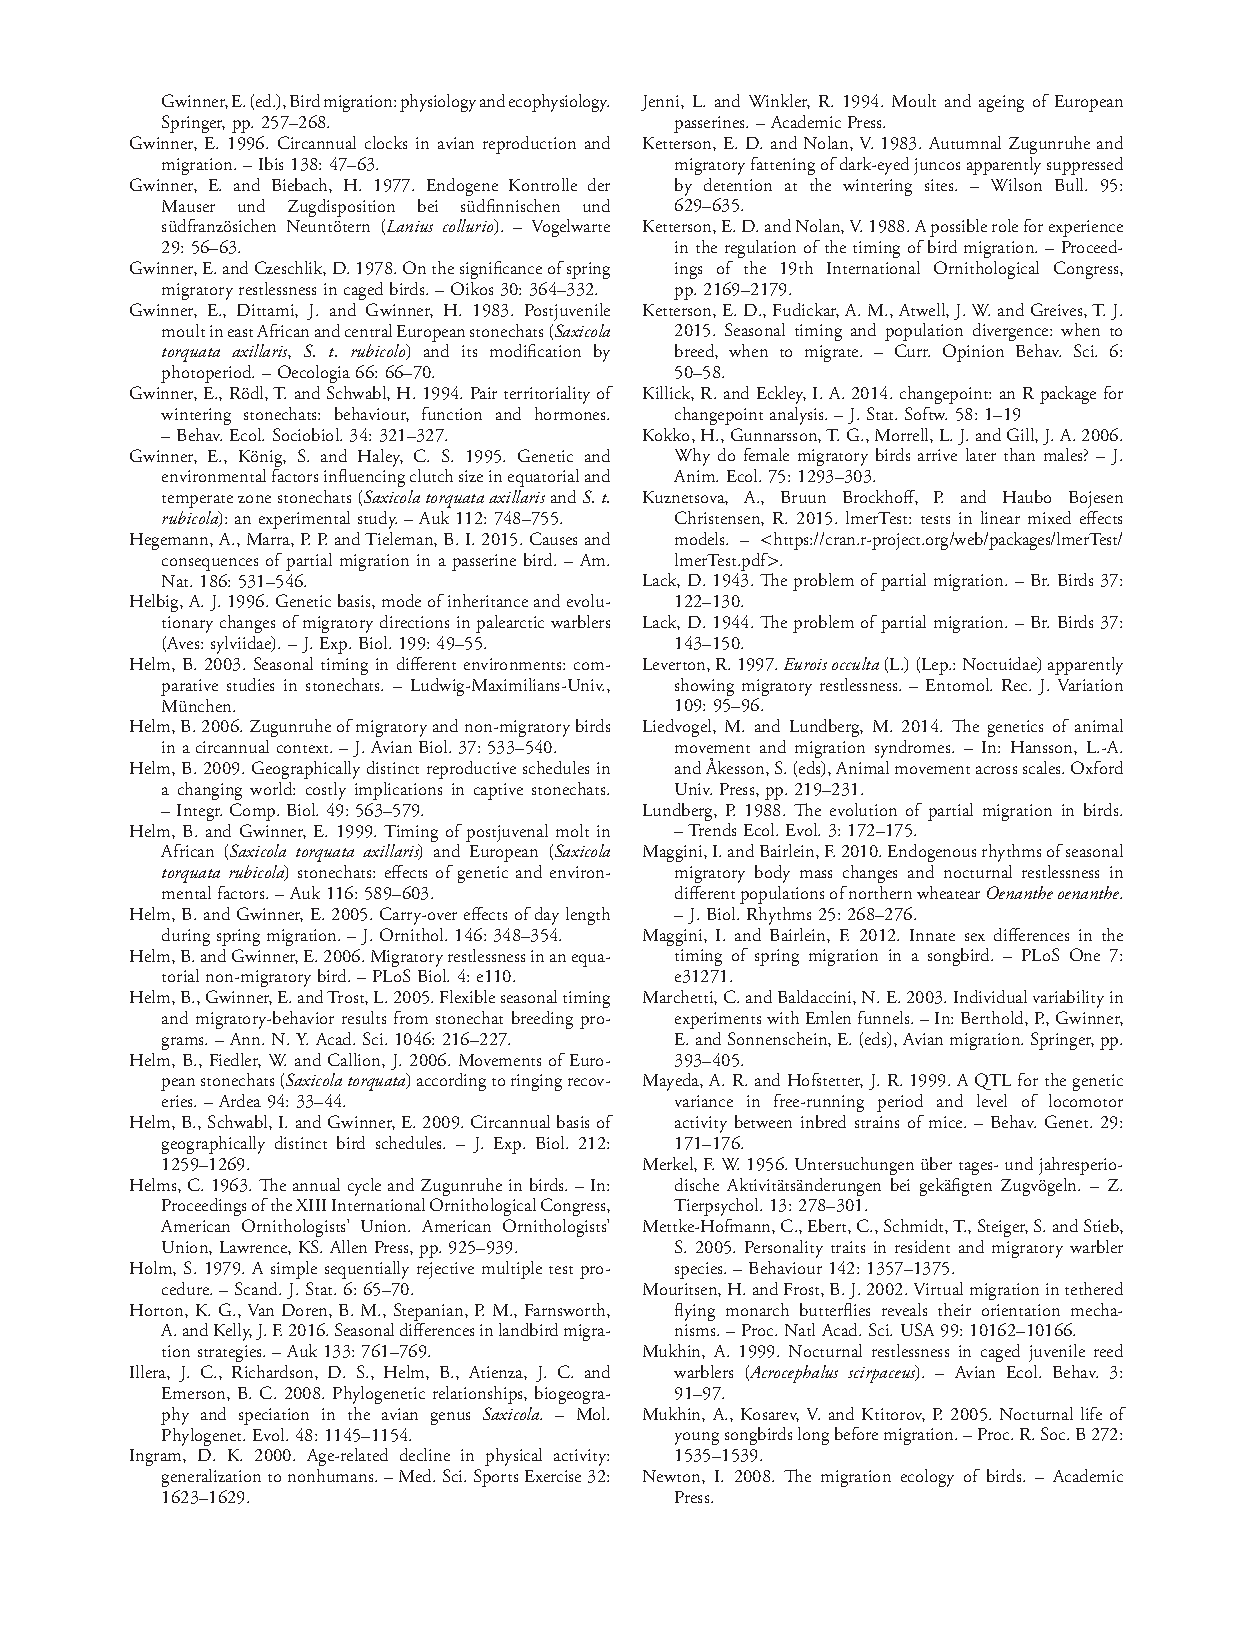
\includegraphics[width=1.15\linewidth]{/Users/Benjamin/Documents/Oxford/Thesis/oxforddown/pdf_chapters/zug/zug_crop_Part17.pdf}} \end{center} \newpage 
 \begin{center} \makebox[\linewidth][c]{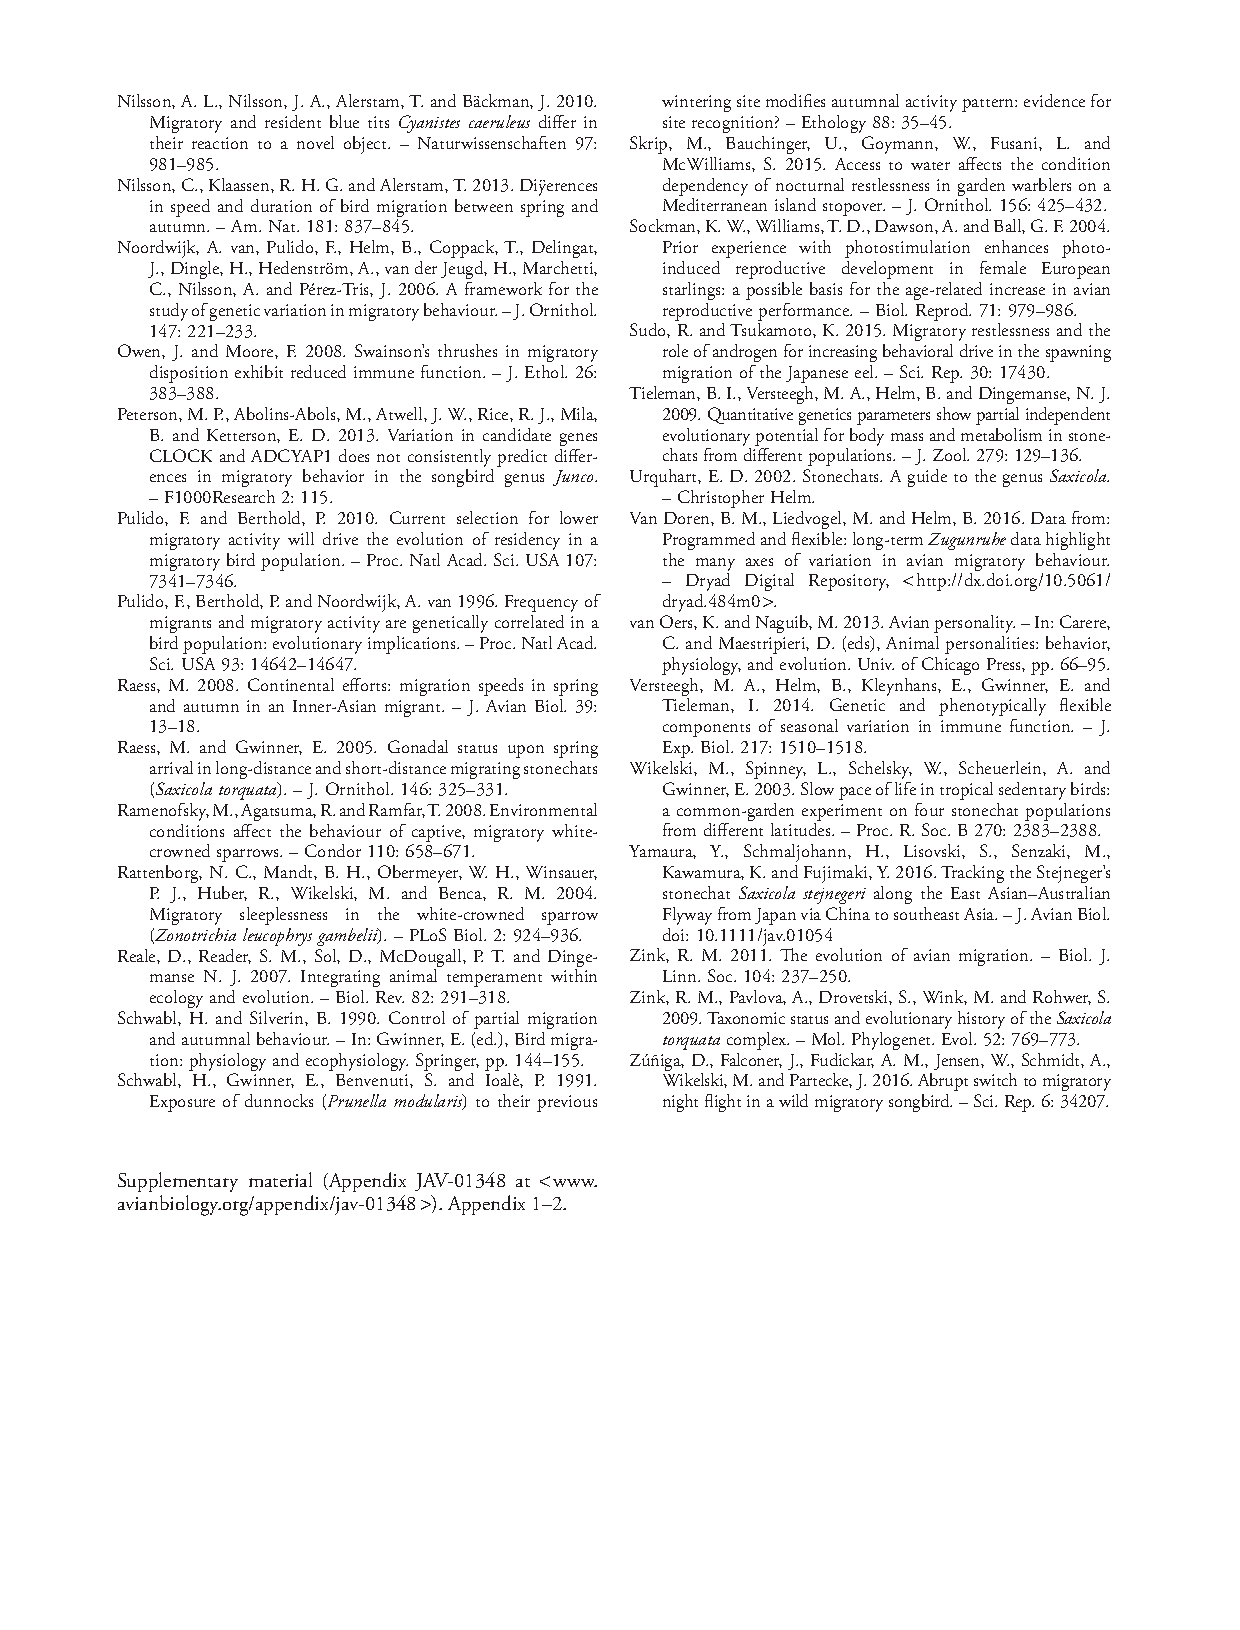
\includegraphics[width=1.15\linewidth]{/Users/Benjamin/Documents/Oxford/Thesis/oxforddown/pdf_chapters/zug/zug_crop_Part18.pdf}} \end{center} \newpage

\begin{savequote}
Helm, B.,* \textbf{Van Doren, B.M.},* Hoffmann, D., and Hoffmann, U.
(2019). Evolutionary response to climate change in migratory pied
flycatchers. \emph{Current Biology} 29, 1--6.

\begin{scriptsize} * Equal contributions. \end{scriptsize}
\end{savequote}

\hypertarget{flycatchers}{%
\chapter{Evolutionary response to climate change in pied flycatchers}\label{flycatchers}}

\chaptermark{Evolutionary response to climate change}

\newpage

\begin{center} \makebox[\linewidth][c]{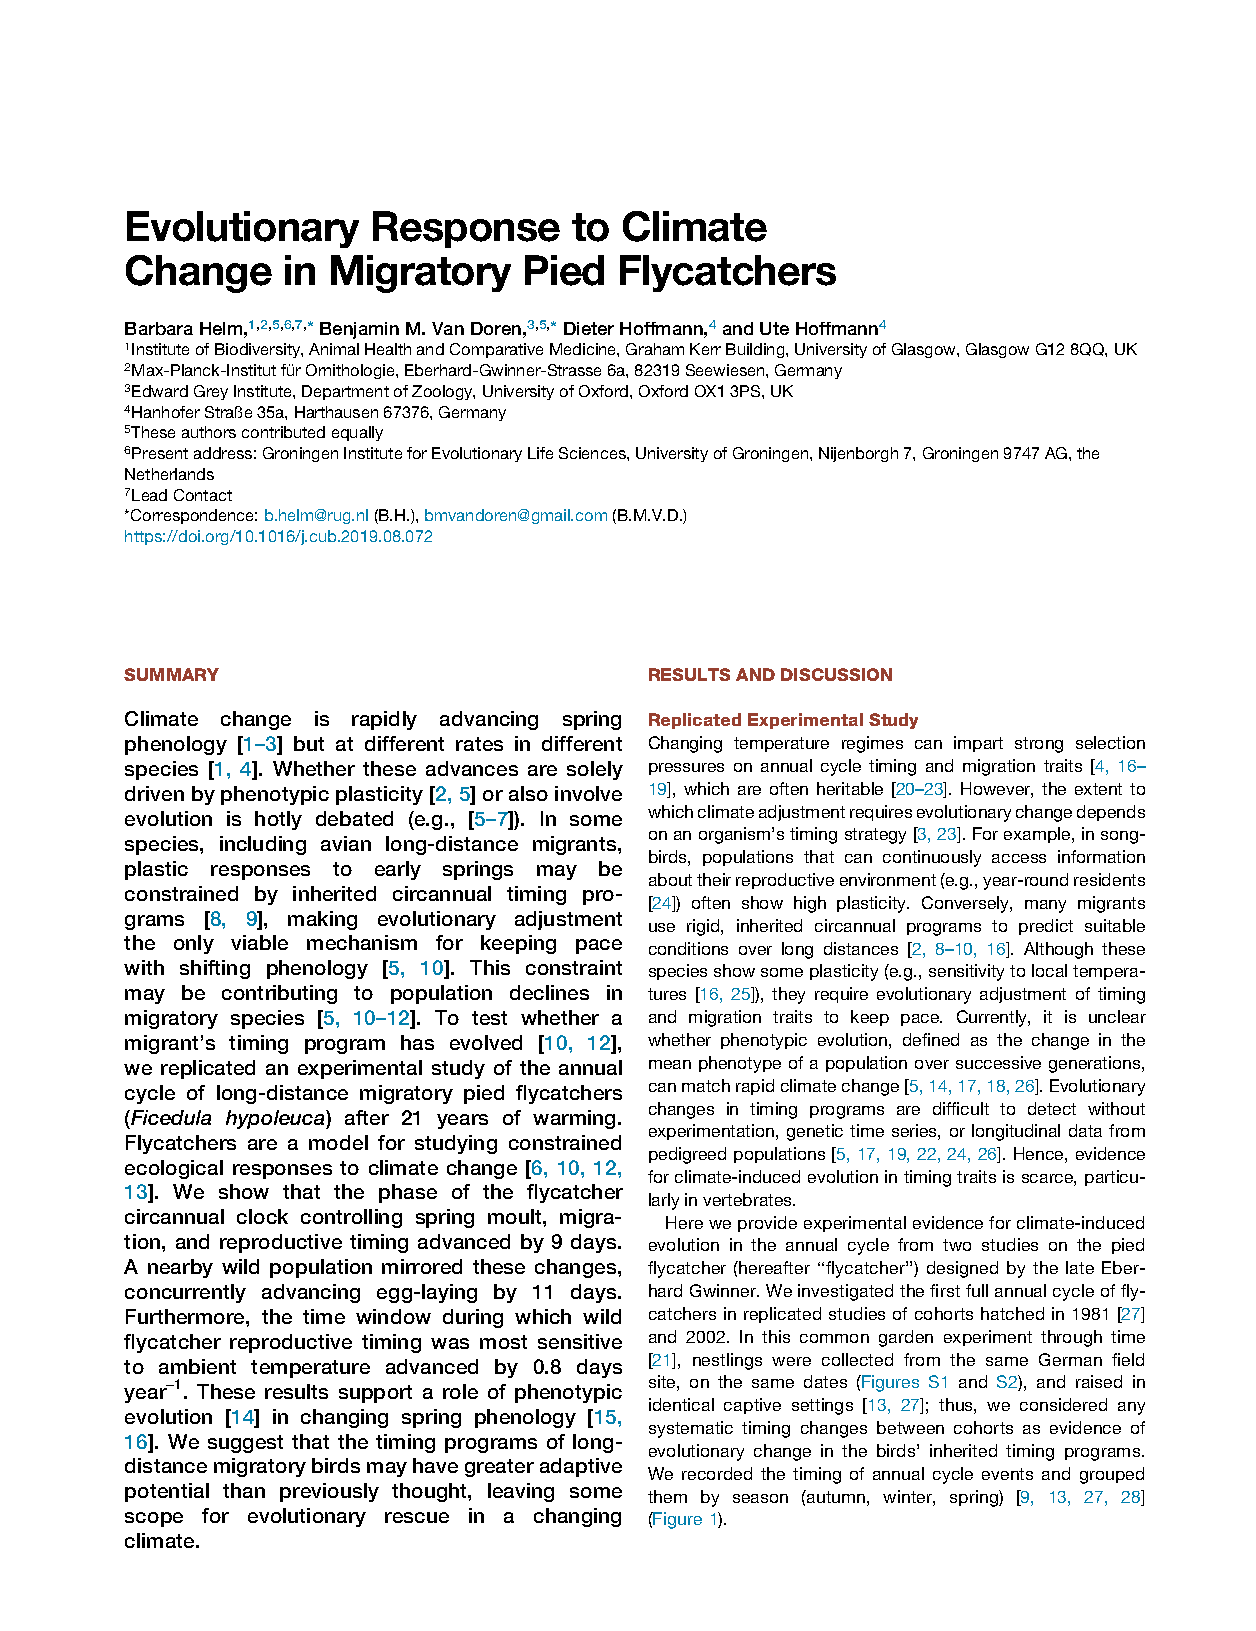
\includegraphics{/Users/Benjamin/Documents/Oxford/Thesis/oxforddown/pdf_chapters/pied/pied_crop_Part01.pdf}} \end{center} \newpage 
 \begin{center} \makebox[\linewidth][c]{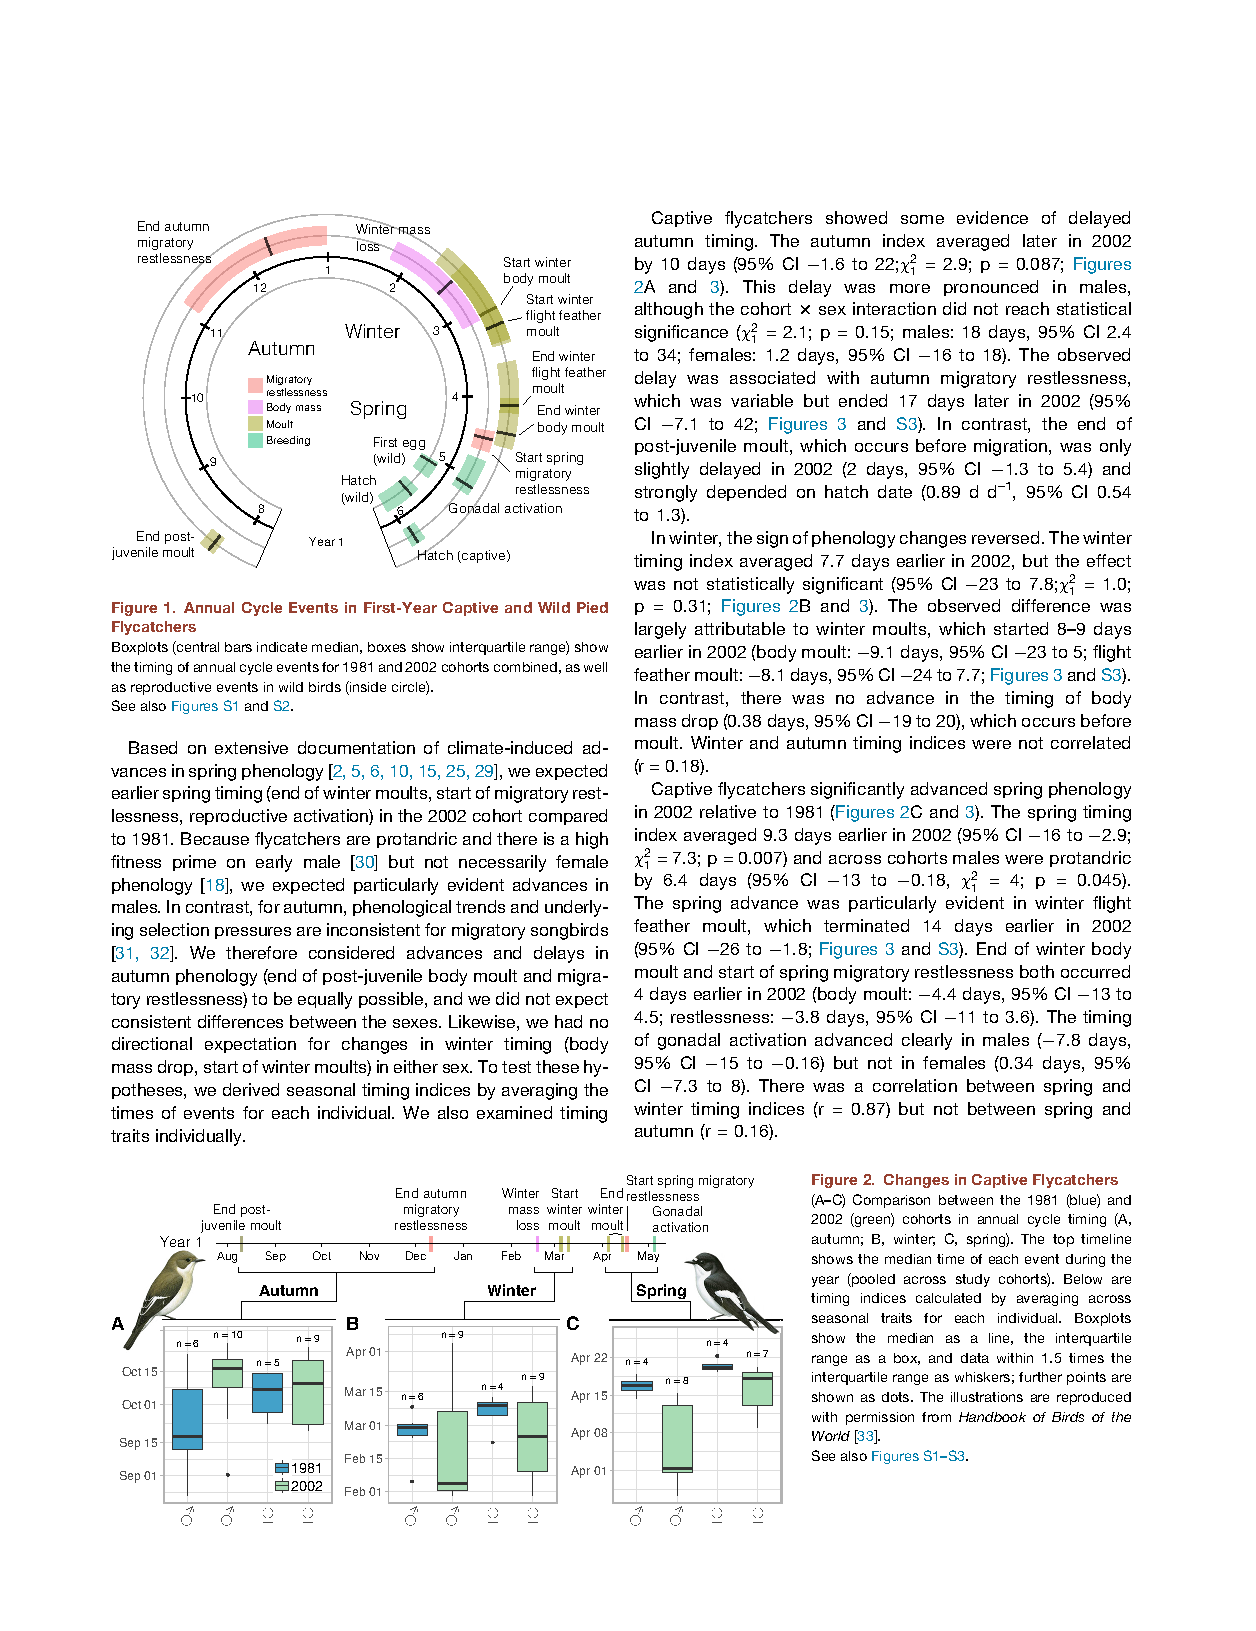
\includegraphics{/Users/Benjamin/Documents/Oxford/Thesis/oxforddown/pdf_chapters/pied/pied_crop_Part02.pdf}} \end{center} \newpage 
 \begin{center} \makebox[\linewidth][c]{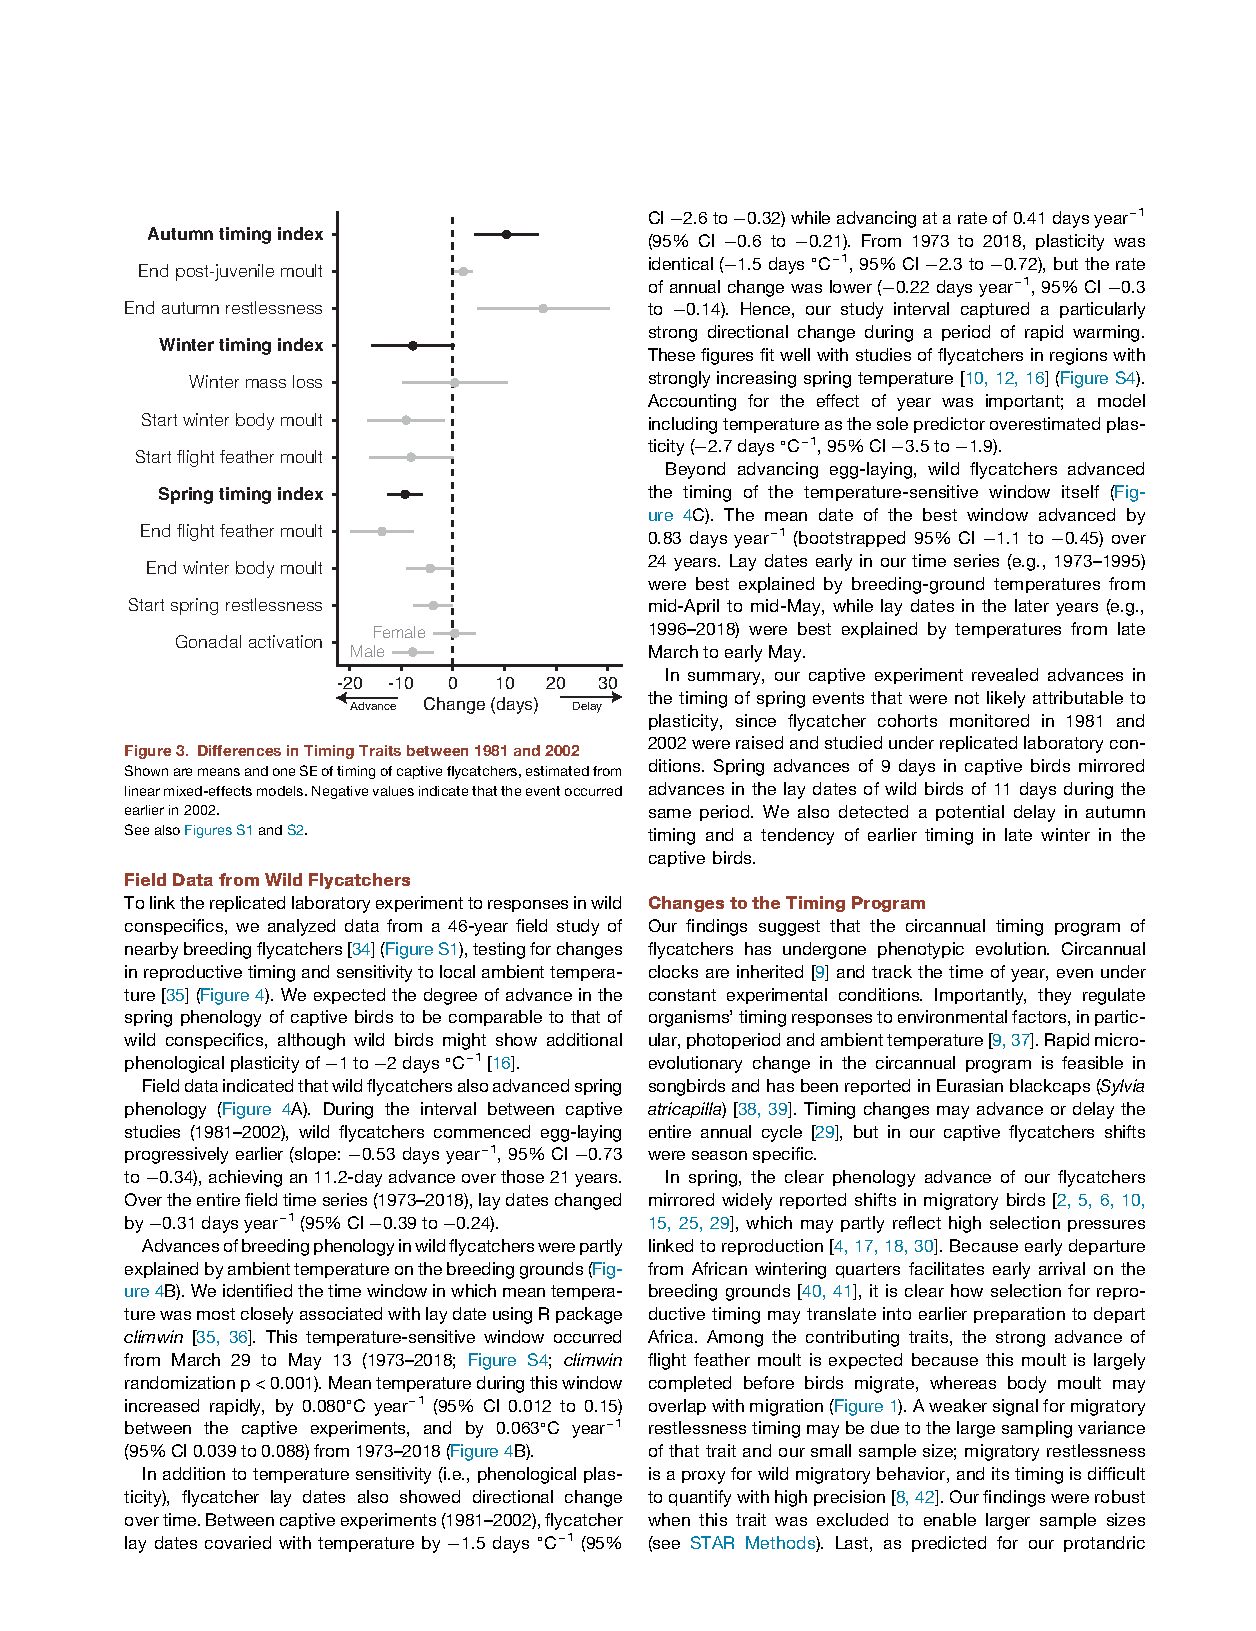
\includegraphics{/Users/Benjamin/Documents/Oxford/Thesis/oxforddown/pdf_chapters/pied/pied_crop_Part03.pdf}} \end{center} \newpage 
 \begin{center} \makebox[\linewidth][c]{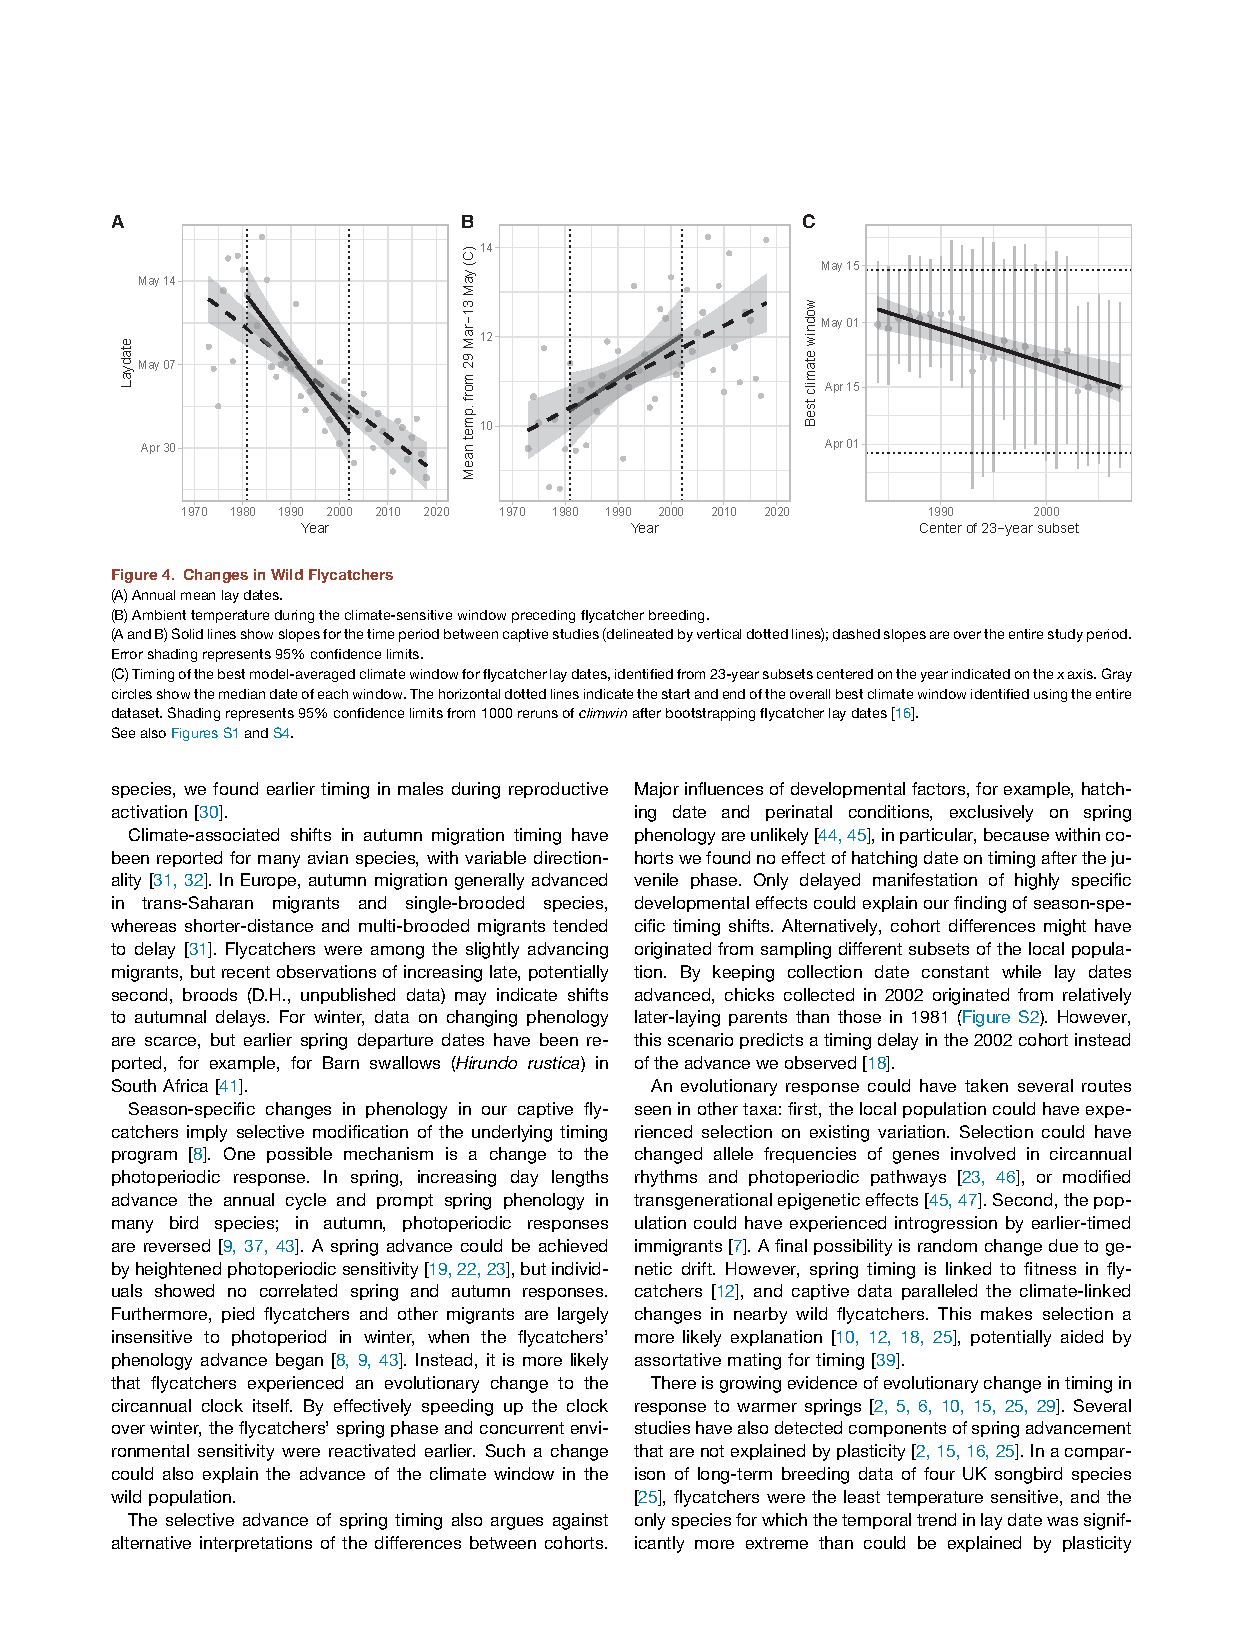
\includegraphics{/Users/Benjamin/Documents/Oxford/Thesis/oxforddown/pdf_chapters/pied/pied_crop_Part04.pdf}} \end{center} \newpage 
 \begin{center} \makebox[\linewidth][c]{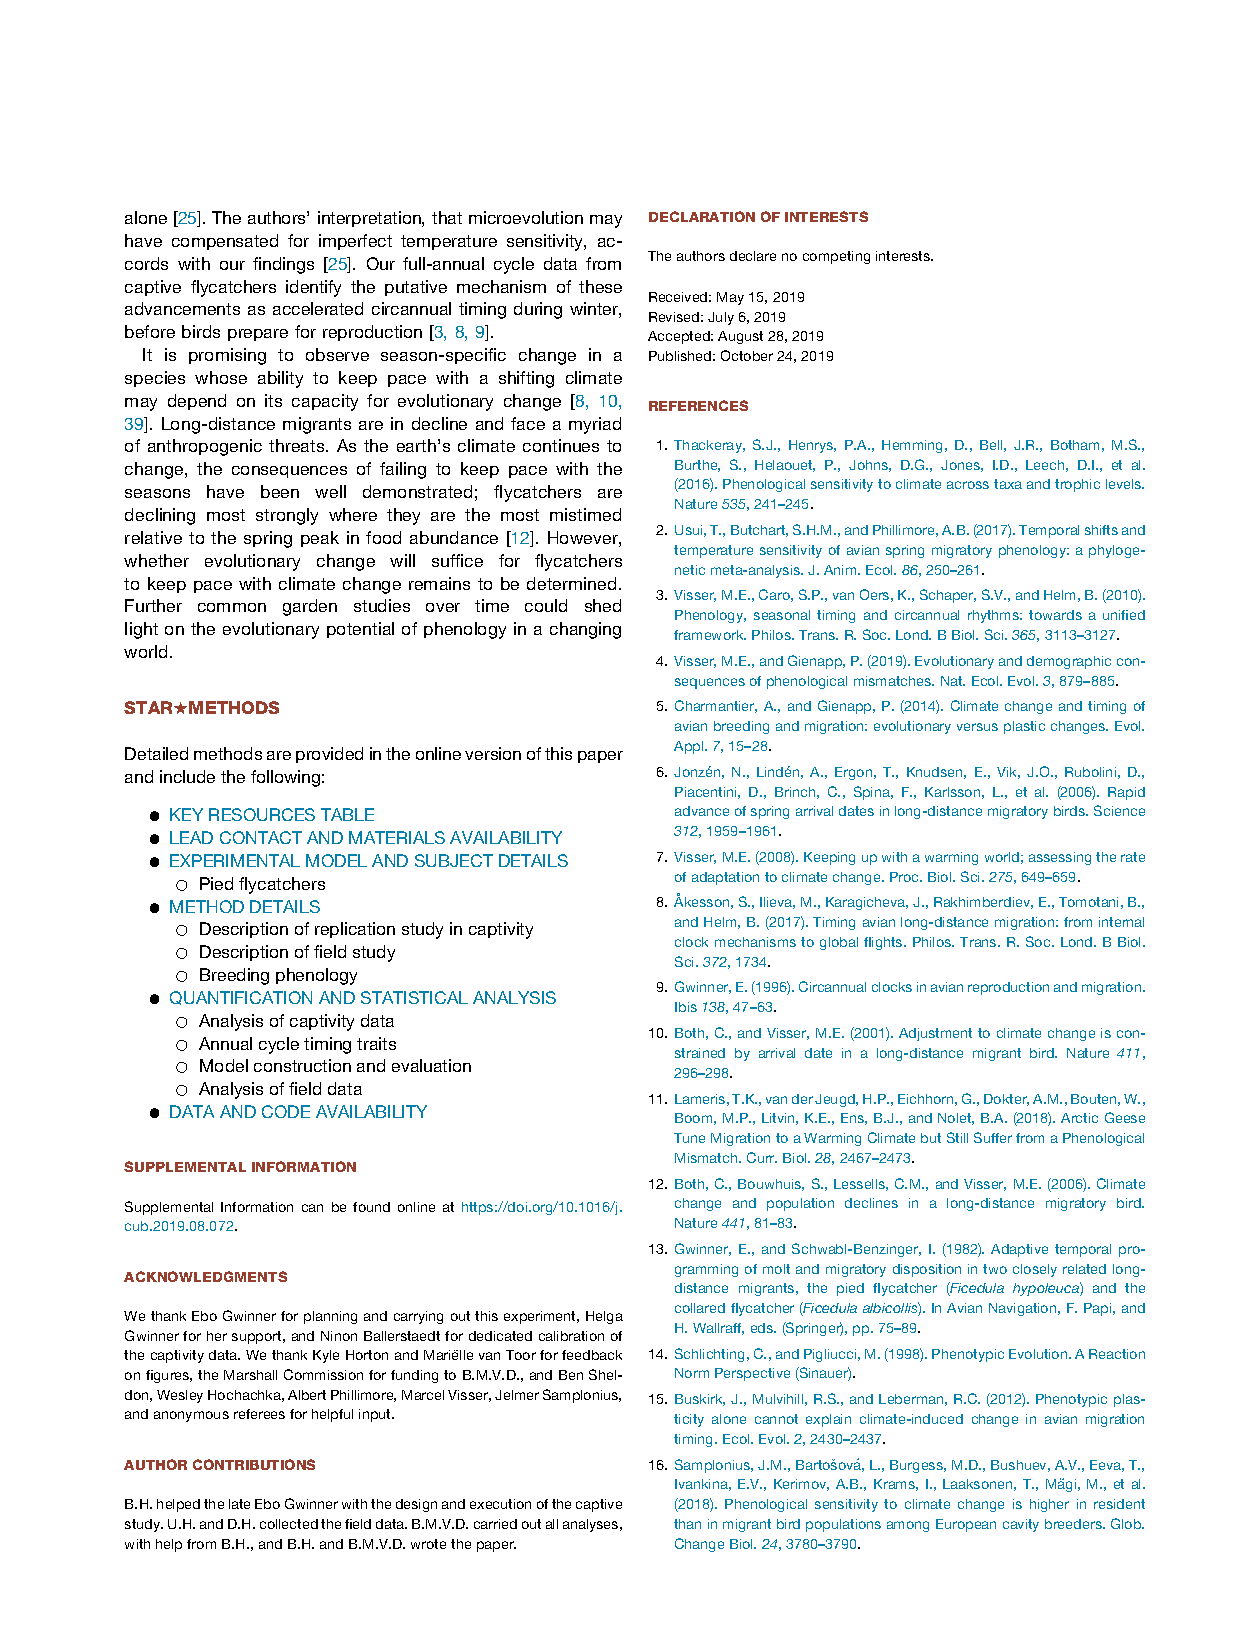
\includegraphics{/Users/Benjamin/Documents/Oxford/Thesis/oxforddown/pdf_chapters/pied/pied_crop_Part05.pdf}} \end{center} \newpage 
 \begin{center} \makebox[\linewidth][c]{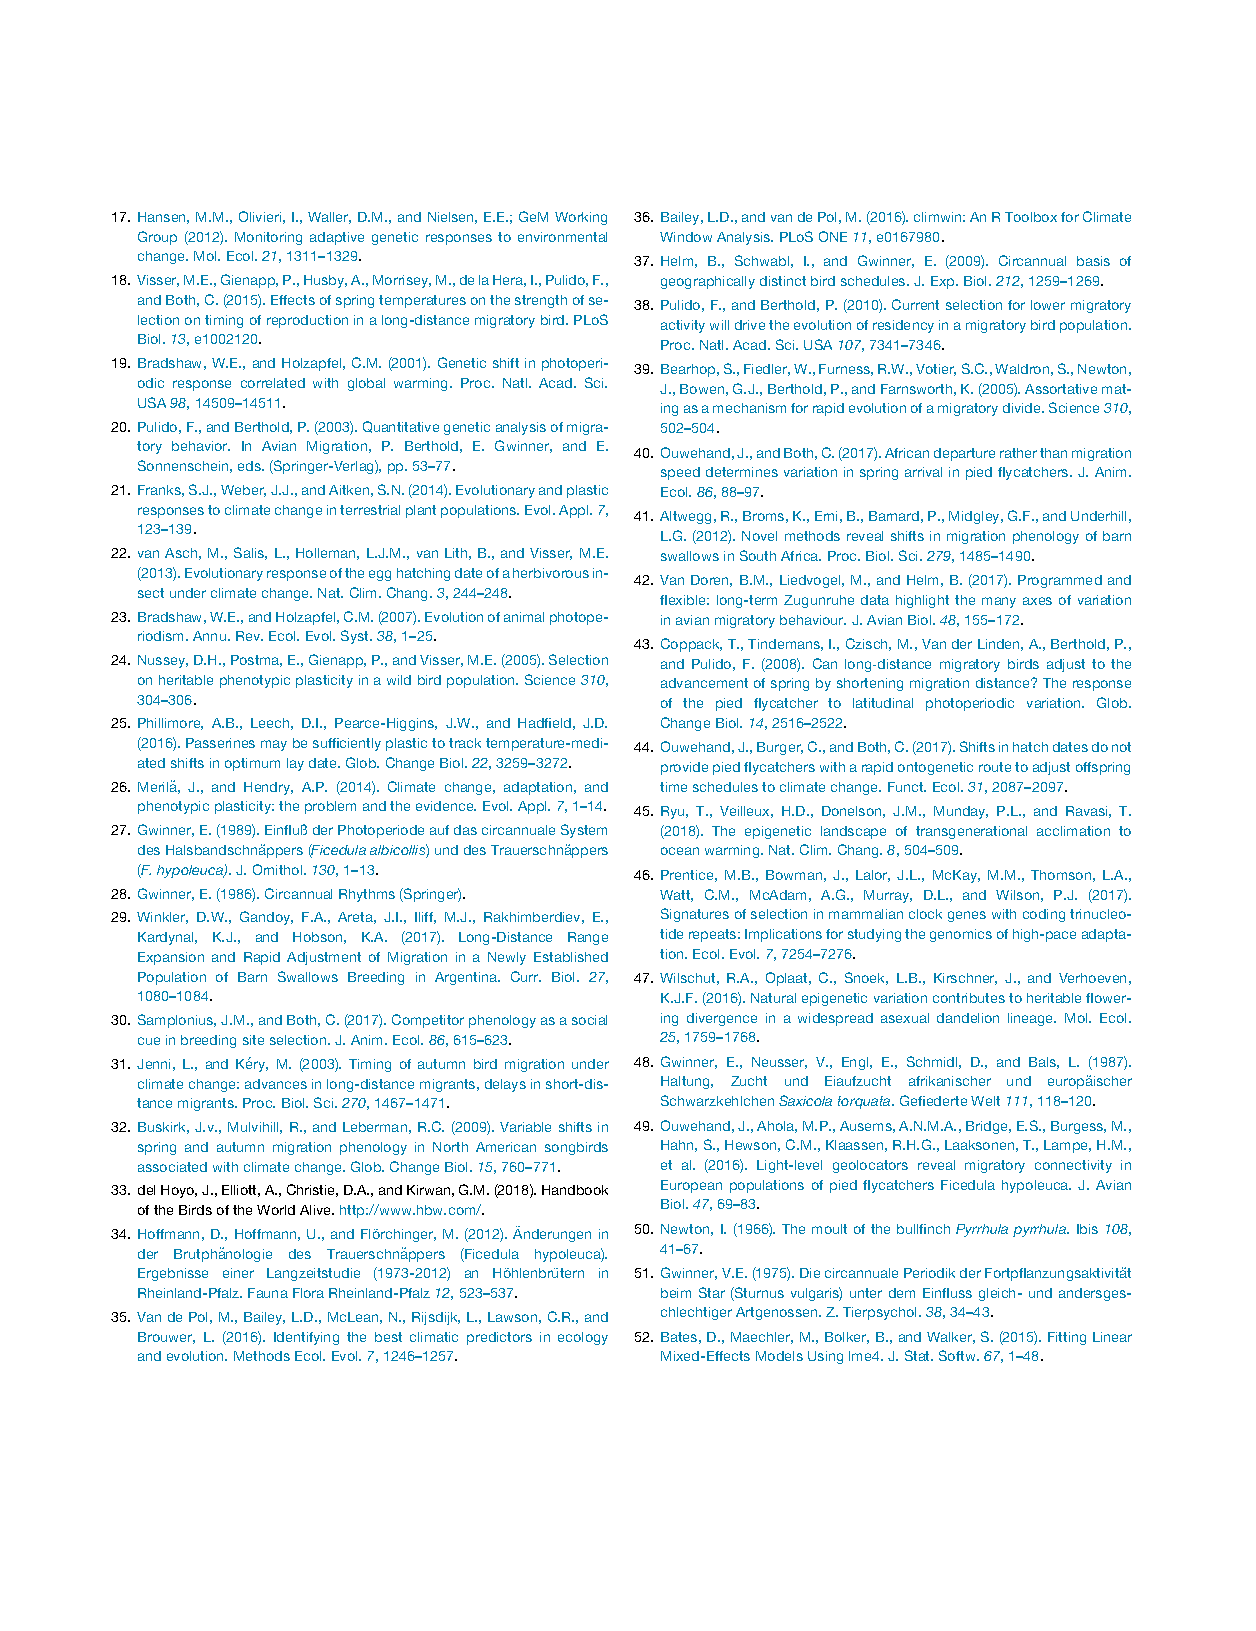
\includegraphics{/Users/Benjamin/Documents/Oxford/Thesis/oxforddown/pdf_chapters/pied/pied_crop_Part06.pdf}} \end{center} \newpage 
 \begin{center} \makebox[\linewidth][c]{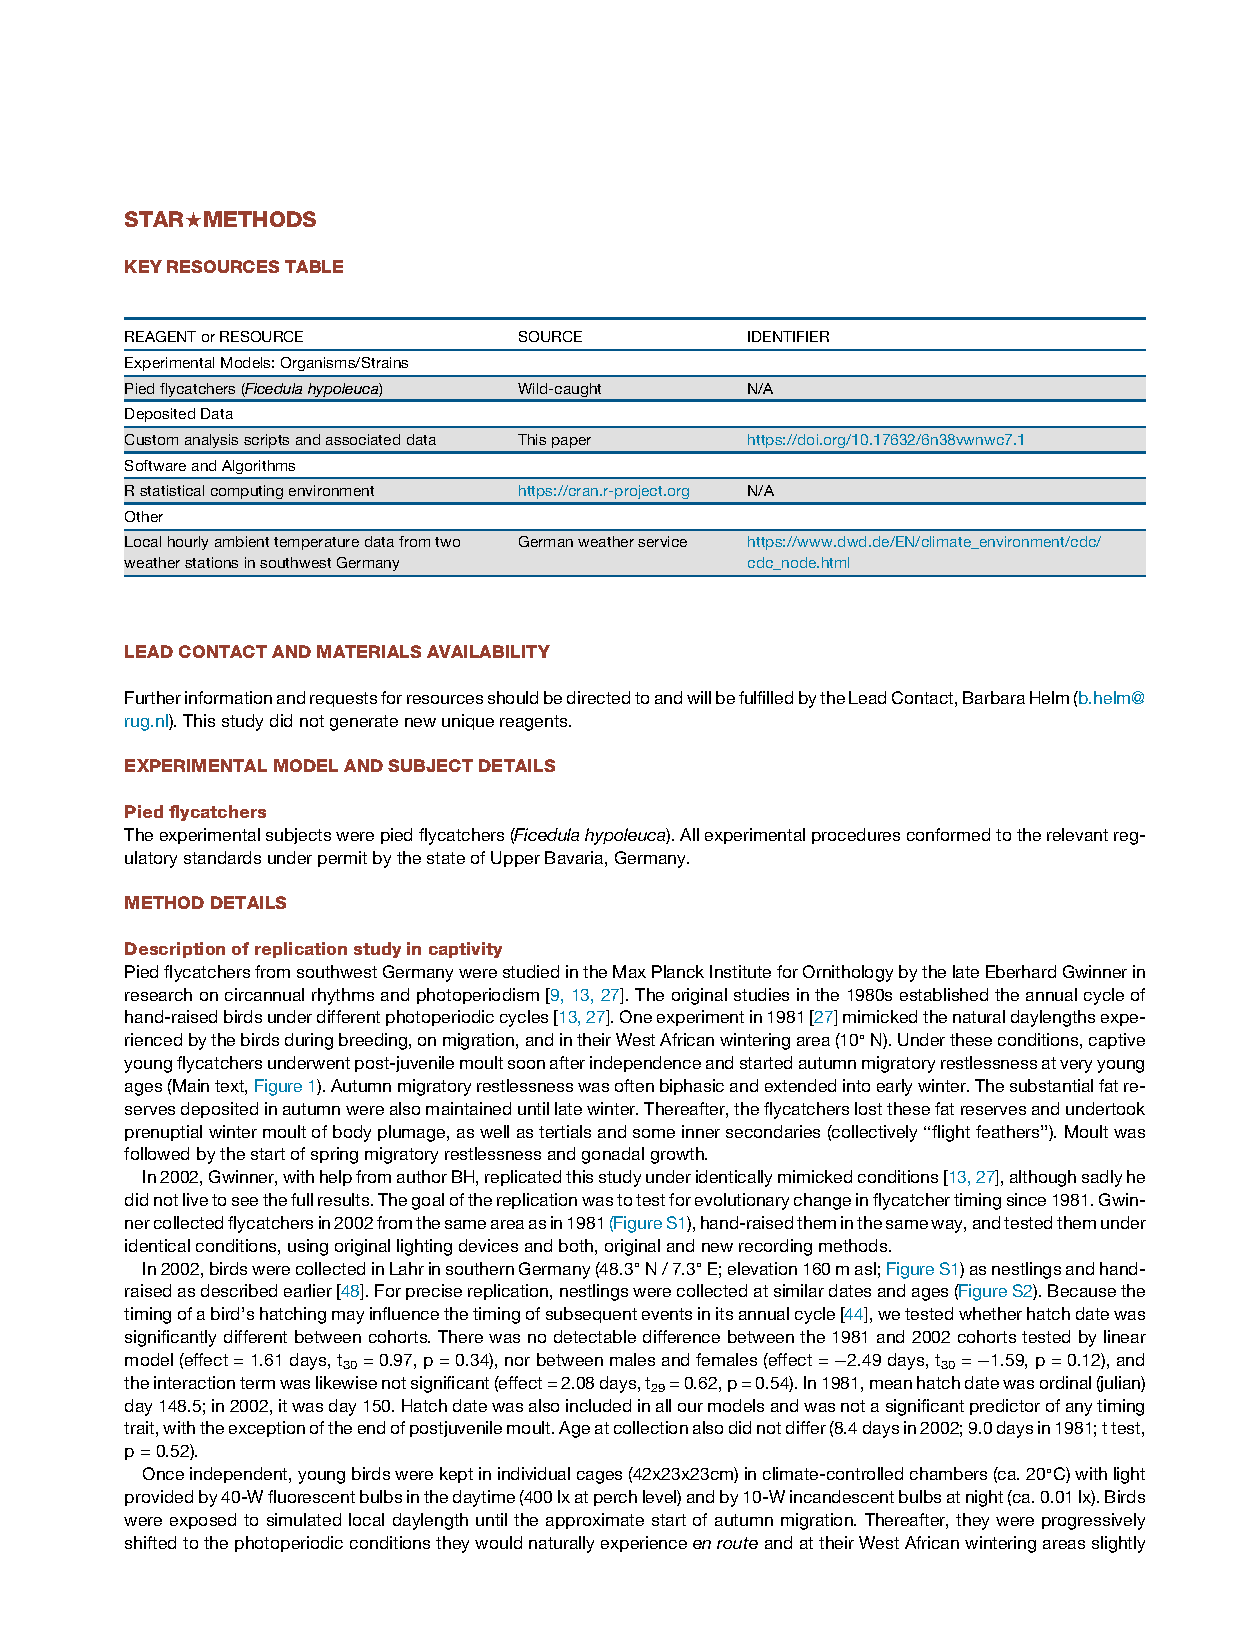
\includegraphics{/Users/Benjamin/Documents/Oxford/Thesis/oxforddown/pdf_chapters/pied/pied_crop_Part07.pdf}} \end{center} \newpage 
 \begin{center} \makebox[\linewidth][c]{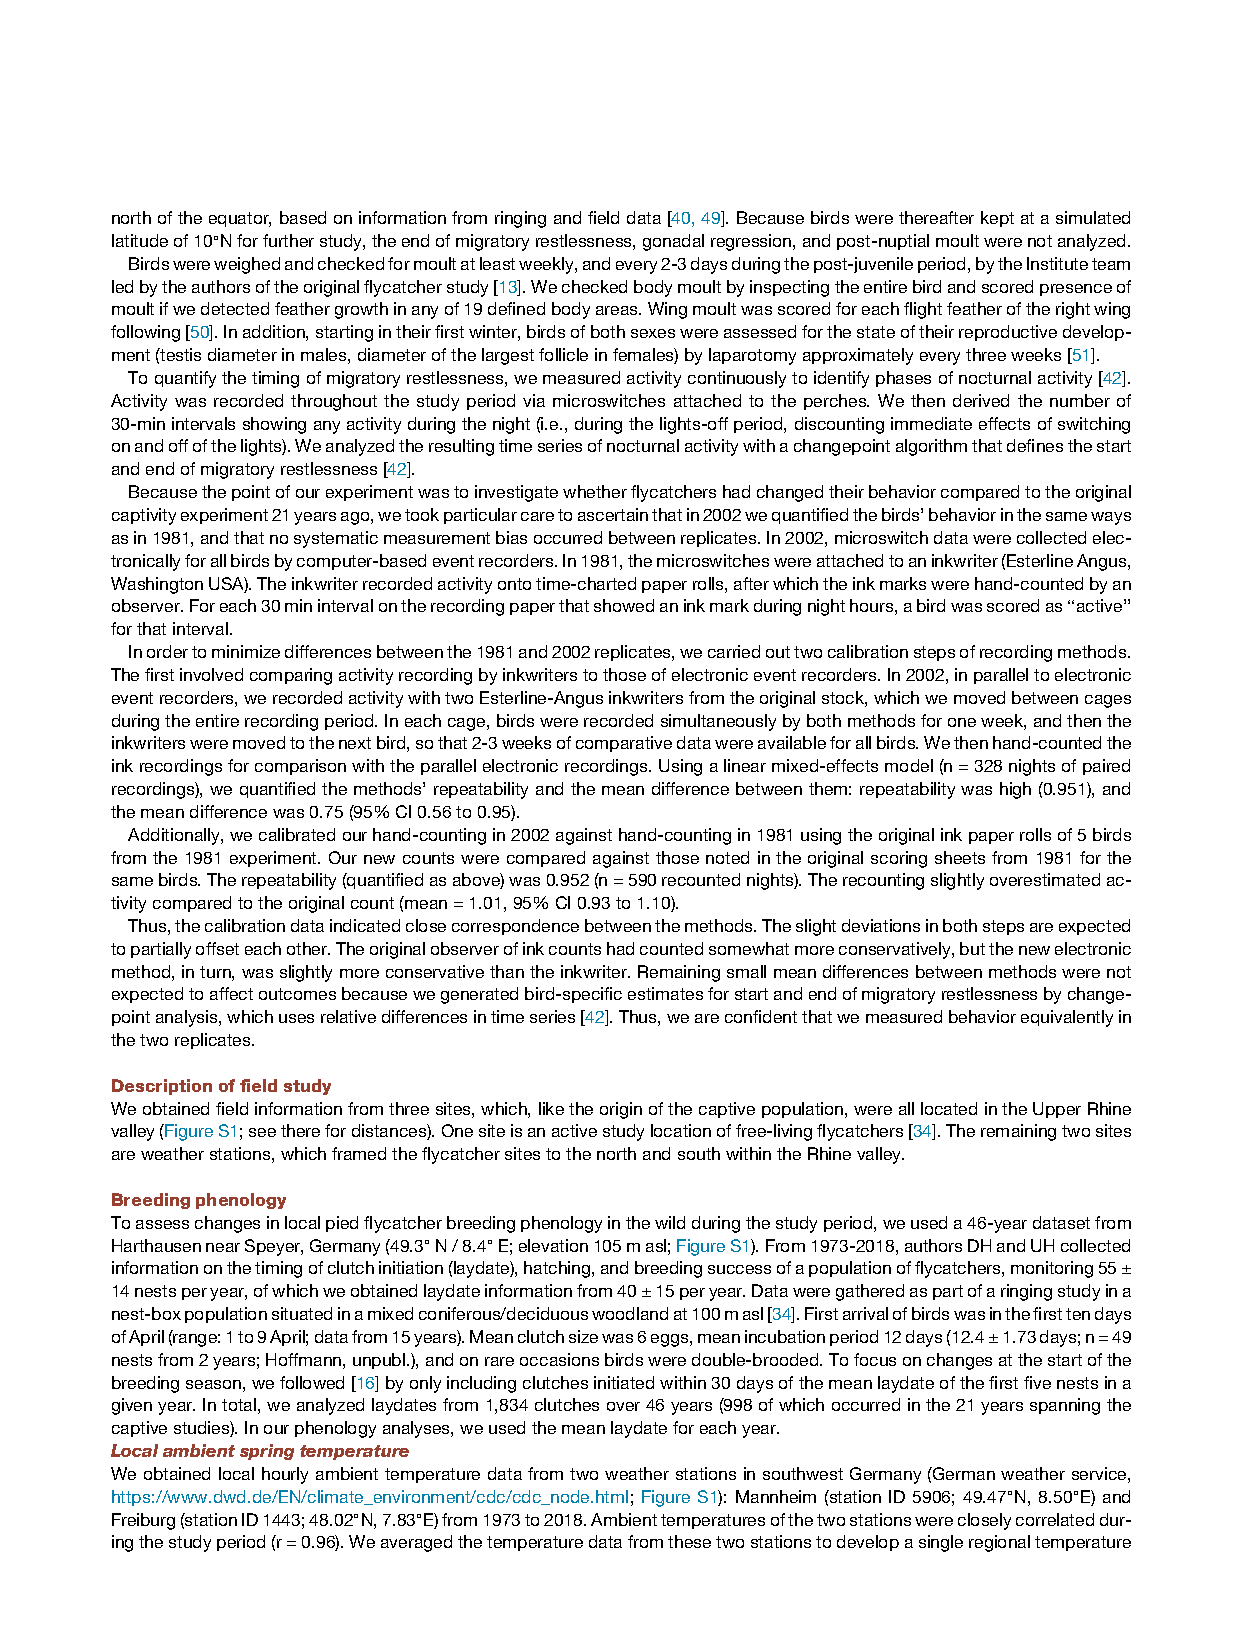
\includegraphics{/Users/Benjamin/Documents/Oxford/Thesis/oxforddown/pdf_chapters/pied/pied_crop_Part08.pdf}} \end{center} \newpage 
 \begin{center} \makebox[\linewidth][c]{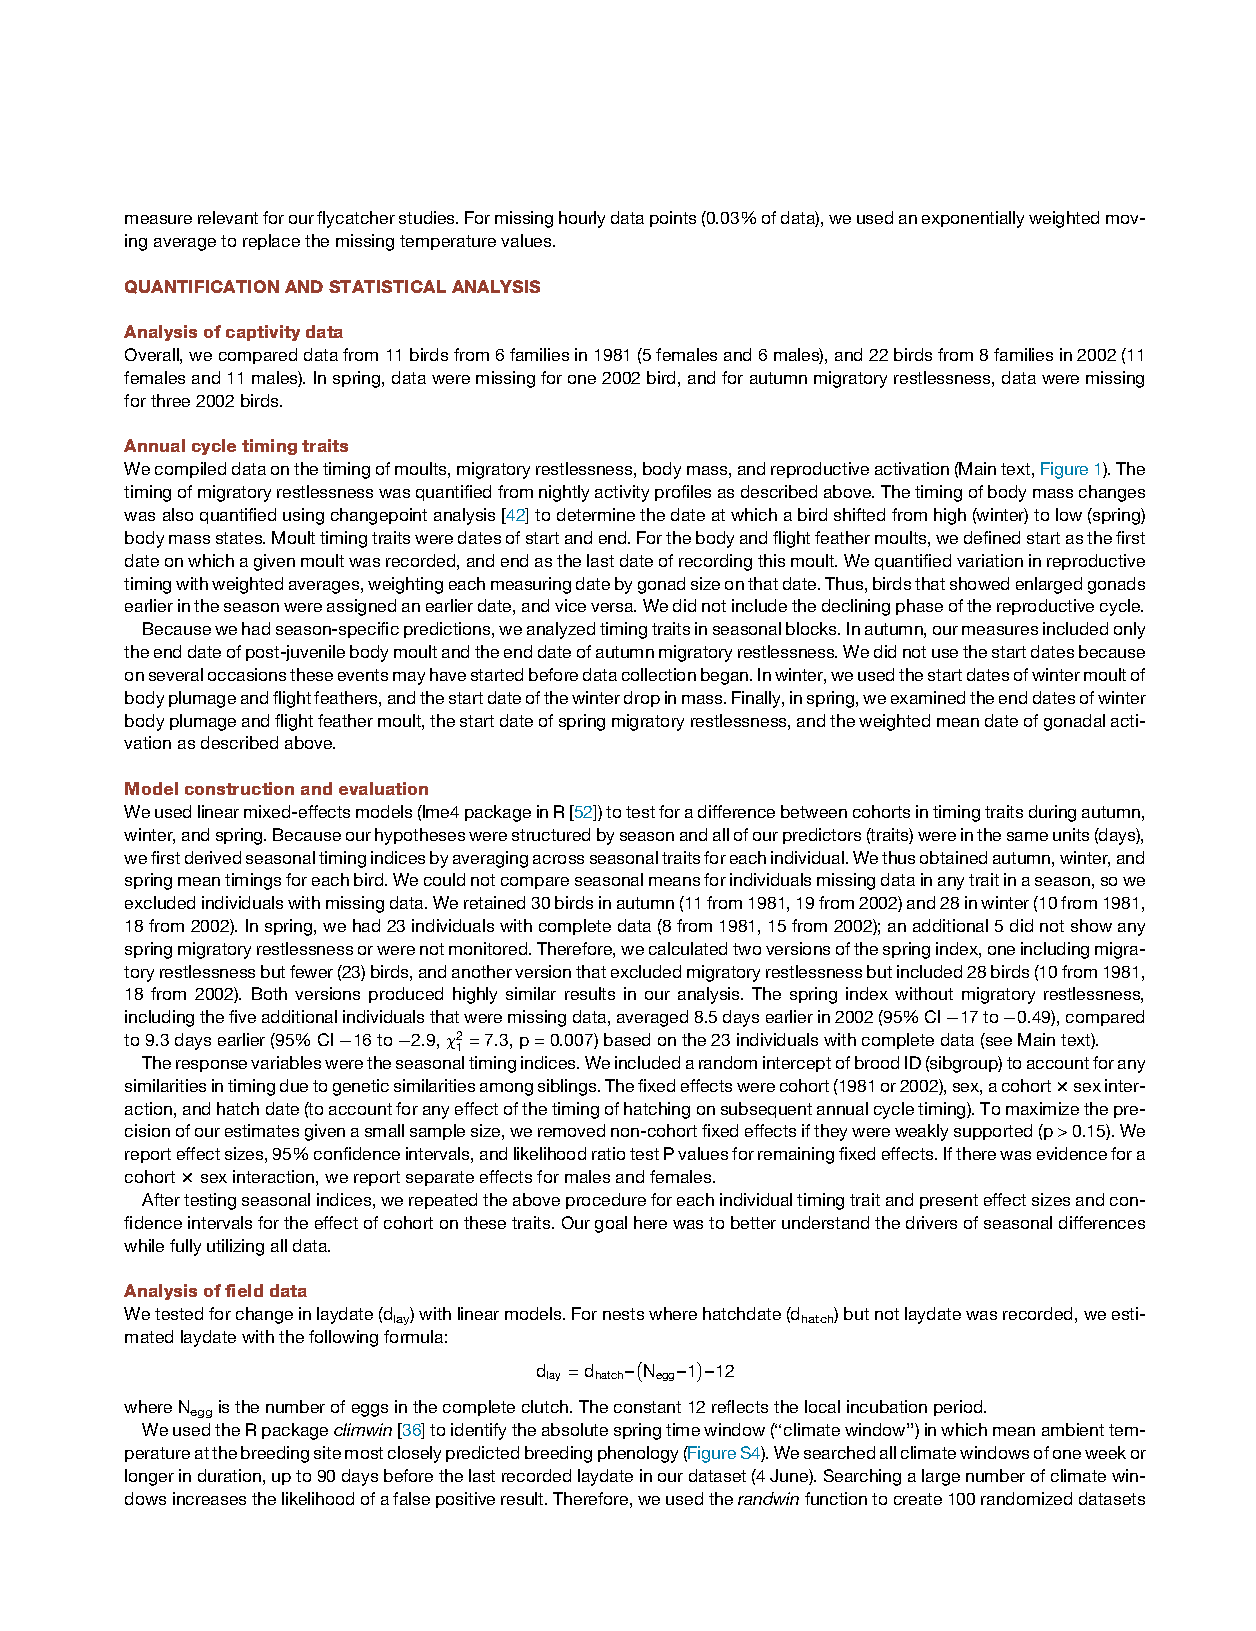
\includegraphics{/Users/Benjamin/Documents/Oxford/Thesis/oxforddown/pdf_chapters/pied/pied_crop_Part09.pdf}} \end{center} \newpage 
 \begin{center} \makebox[\linewidth][c]{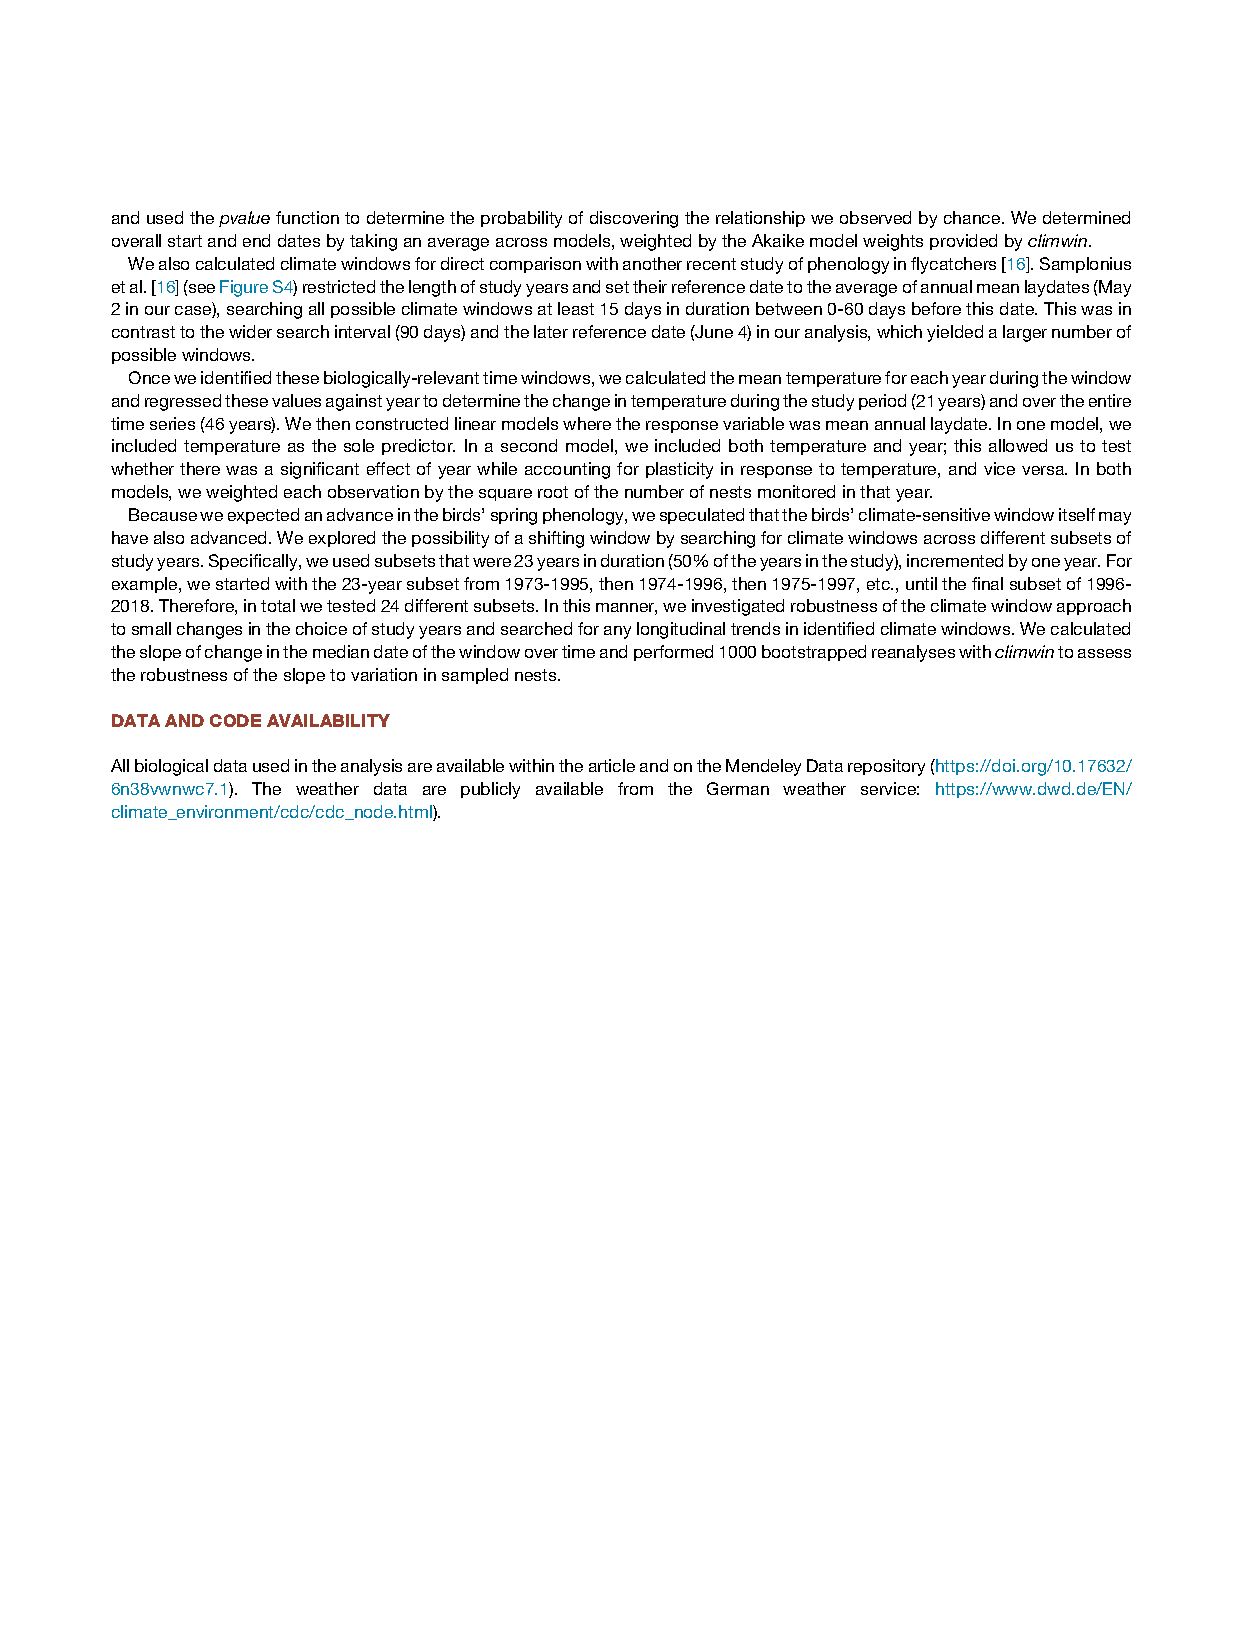
\includegraphics{/Users/Benjamin/Documents/Oxford/Thesis/oxforddown/pdf_chapters/pied/pied_crop_Part10.pdf}} \end{center} \newpage

\begin{center} 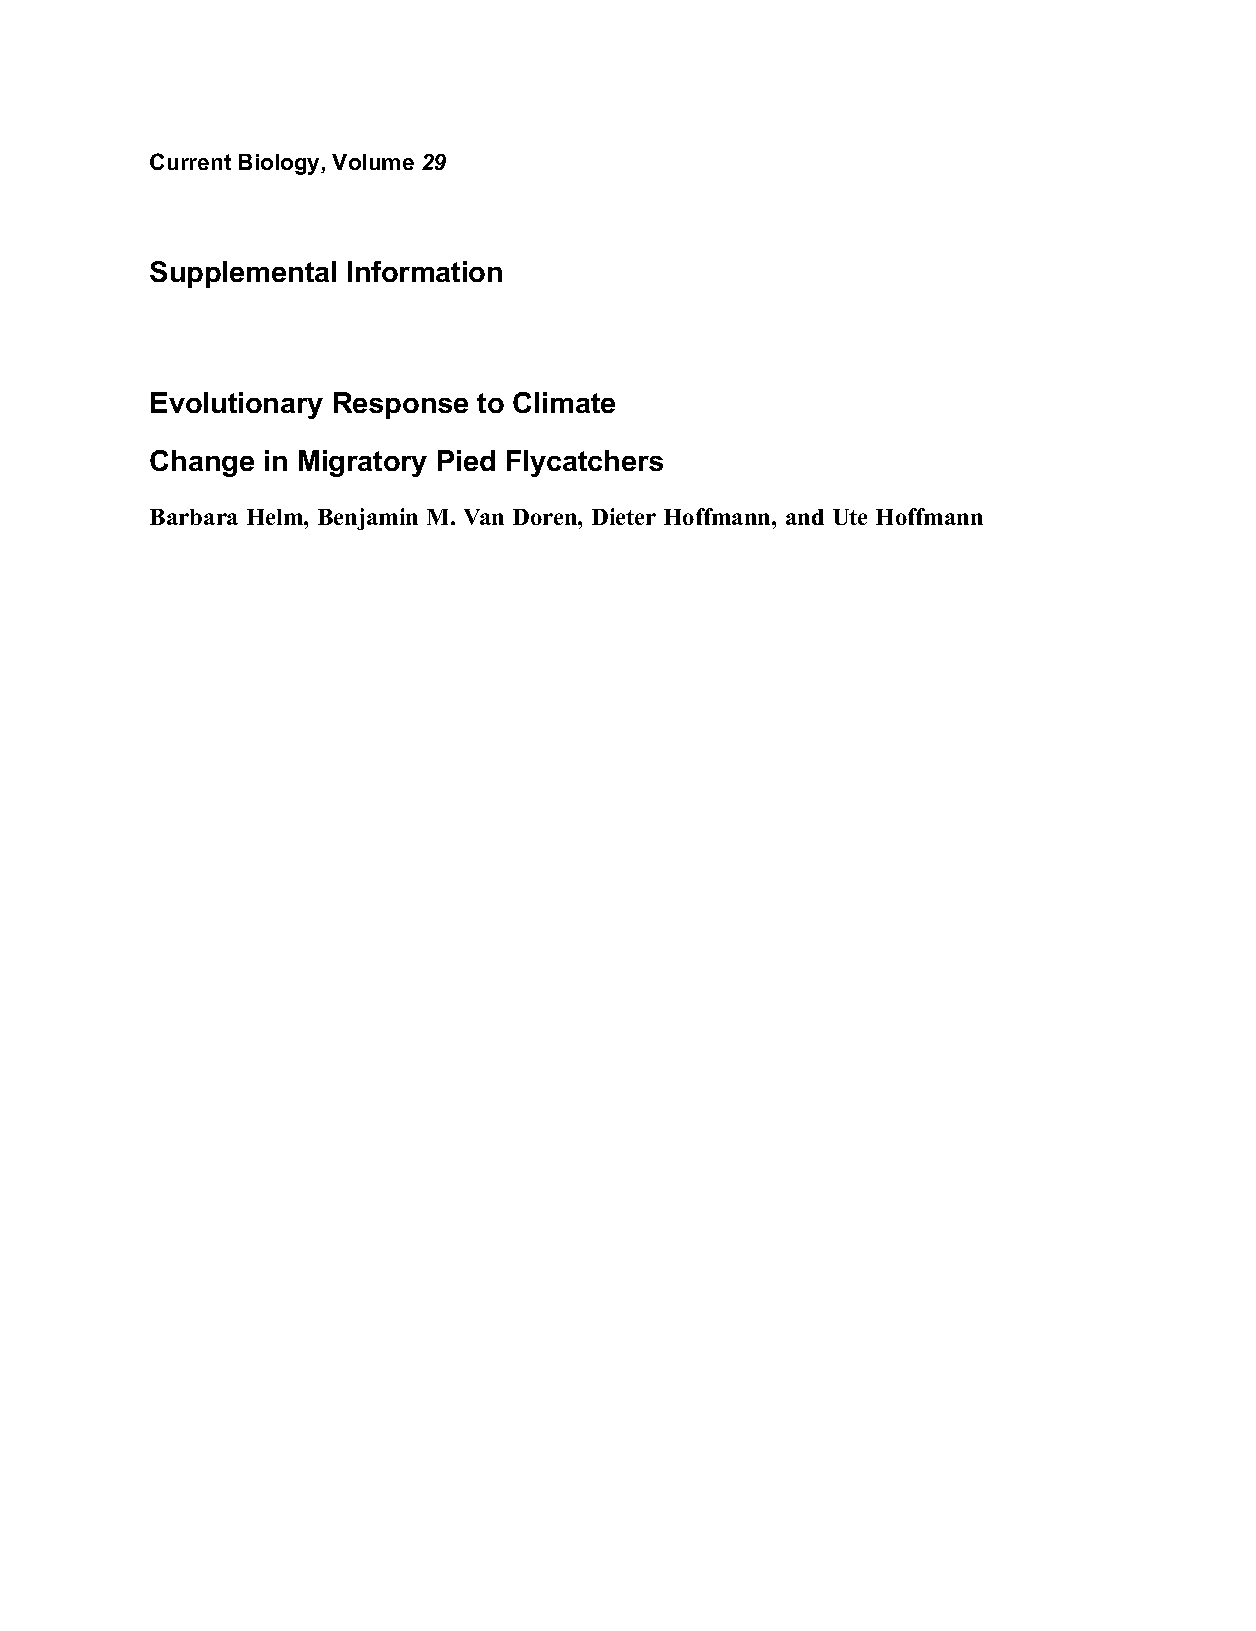
\includegraphics[width=1\linewidth]{/Users/Benjamin/Documents/Oxford/Thesis/oxforddown/pdf_chapters/pied/pied_supp_crop_Part1.pdf} \end{center} \newpage 
 \begin{center} 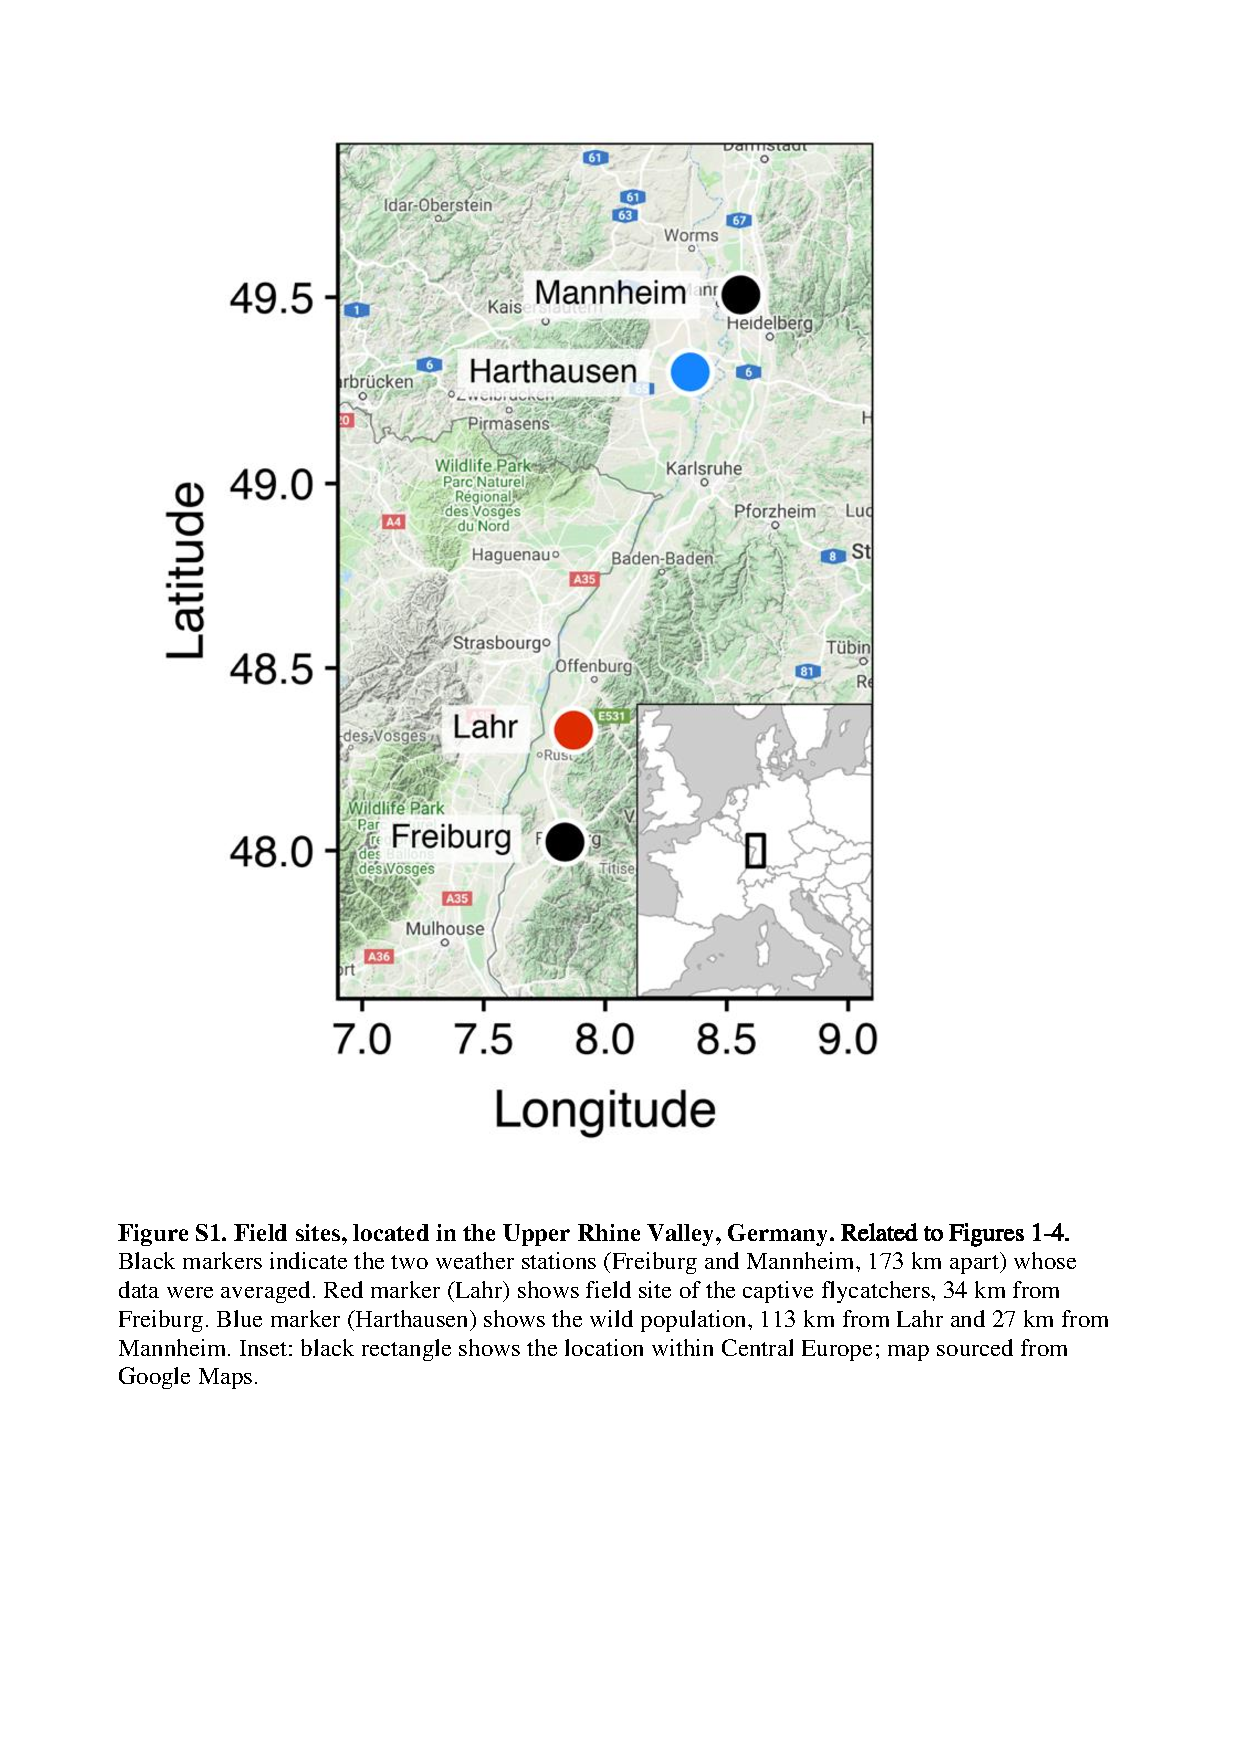
\includegraphics[width=1\linewidth]{/Users/Benjamin/Documents/Oxford/Thesis/oxforddown/pdf_chapters/pied/pied_supp_crop_Part2.pdf} \end{center} \newpage 
 \begin{center} 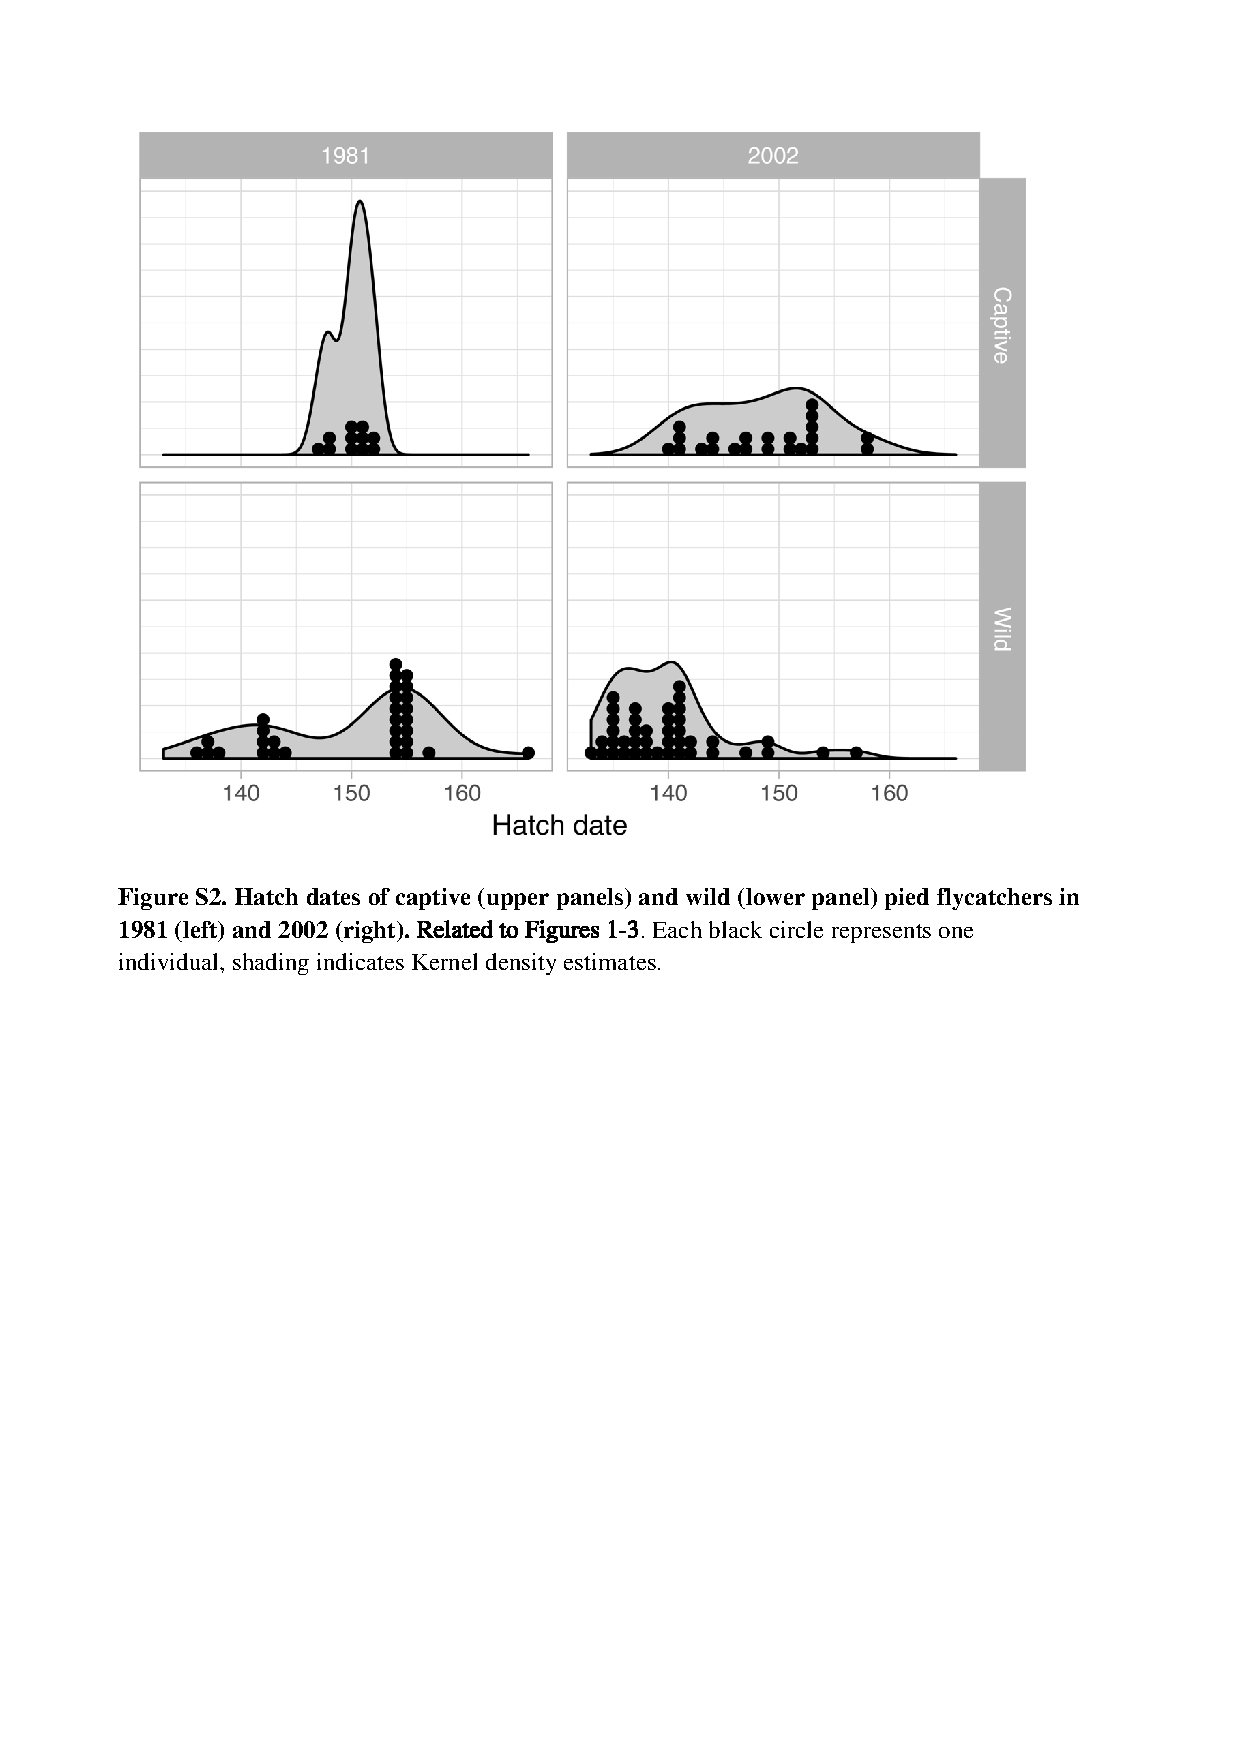
\includegraphics[width=1\linewidth]{/Users/Benjamin/Documents/Oxford/Thesis/oxforddown/pdf_chapters/pied/pied_supp_crop_Part3.pdf} \end{center} \newpage 
 \begin{center} 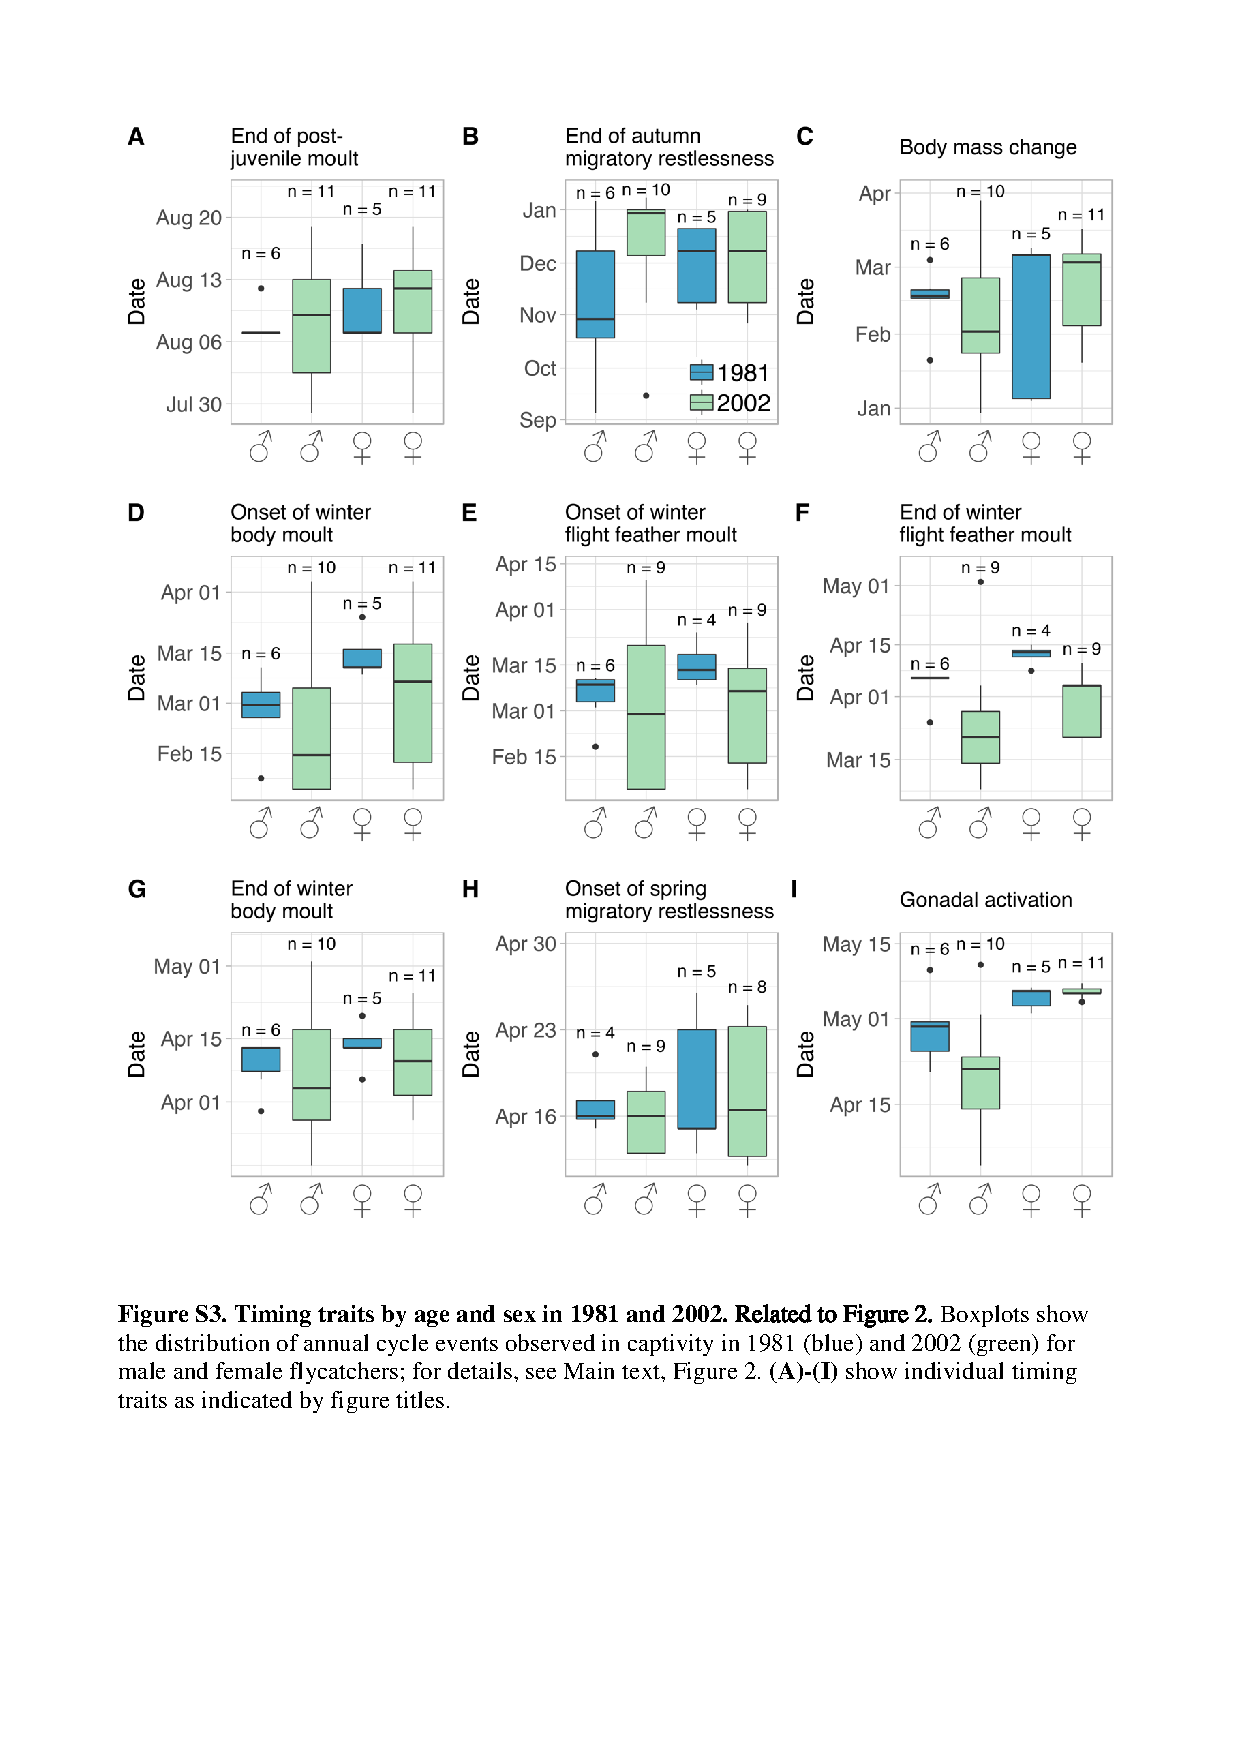
\includegraphics[width=1\linewidth]{/Users/Benjamin/Documents/Oxford/Thesis/oxforddown/pdf_chapters/pied/pied_supp_crop_Part4.pdf} \end{center} \newpage 
 \begin{center} 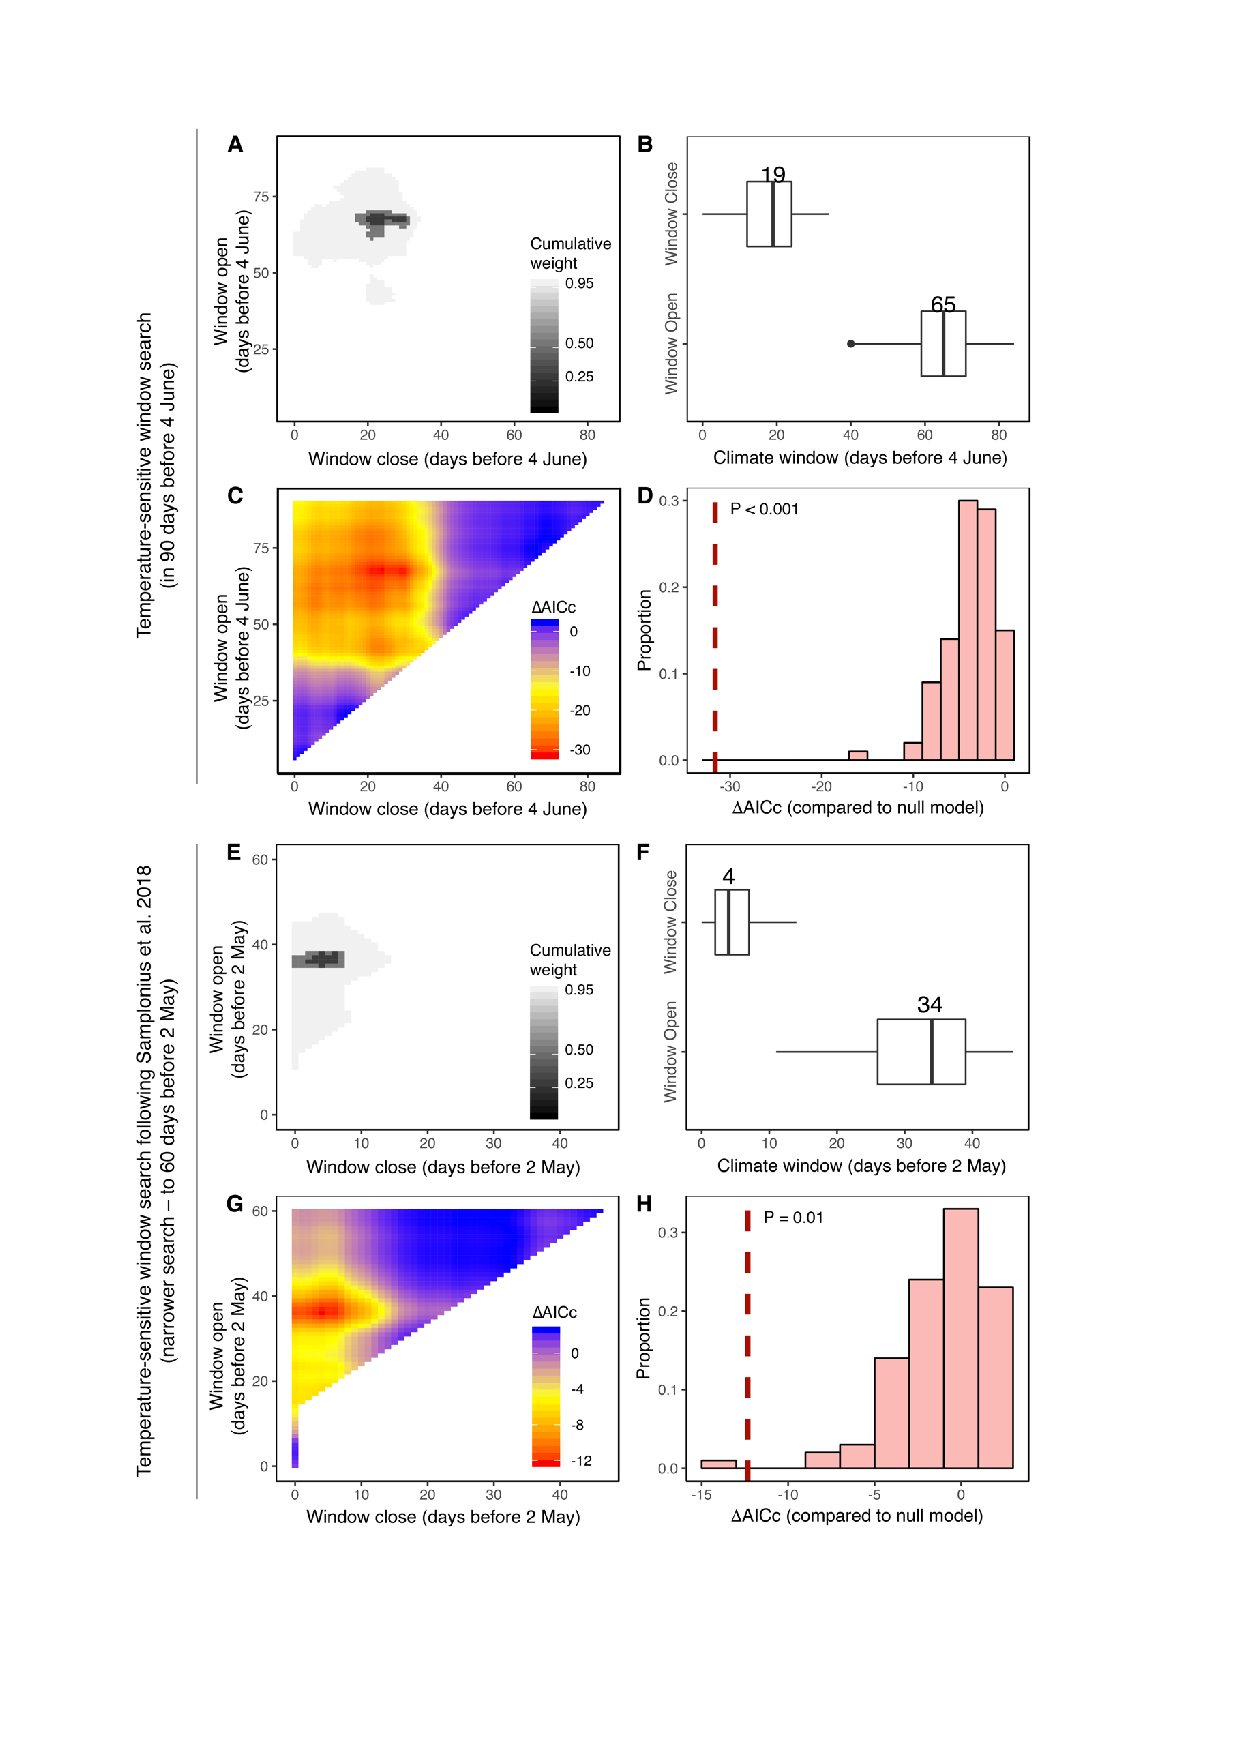
\includegraphics[width=1\linewidth]{/Users/Benjamin/Documents/Oxford/Thesis/oxforddown/pdf_chapters/pied/pied_supp_crop_Part5.pdf} \end{center} \newpage 
 \begin{center} 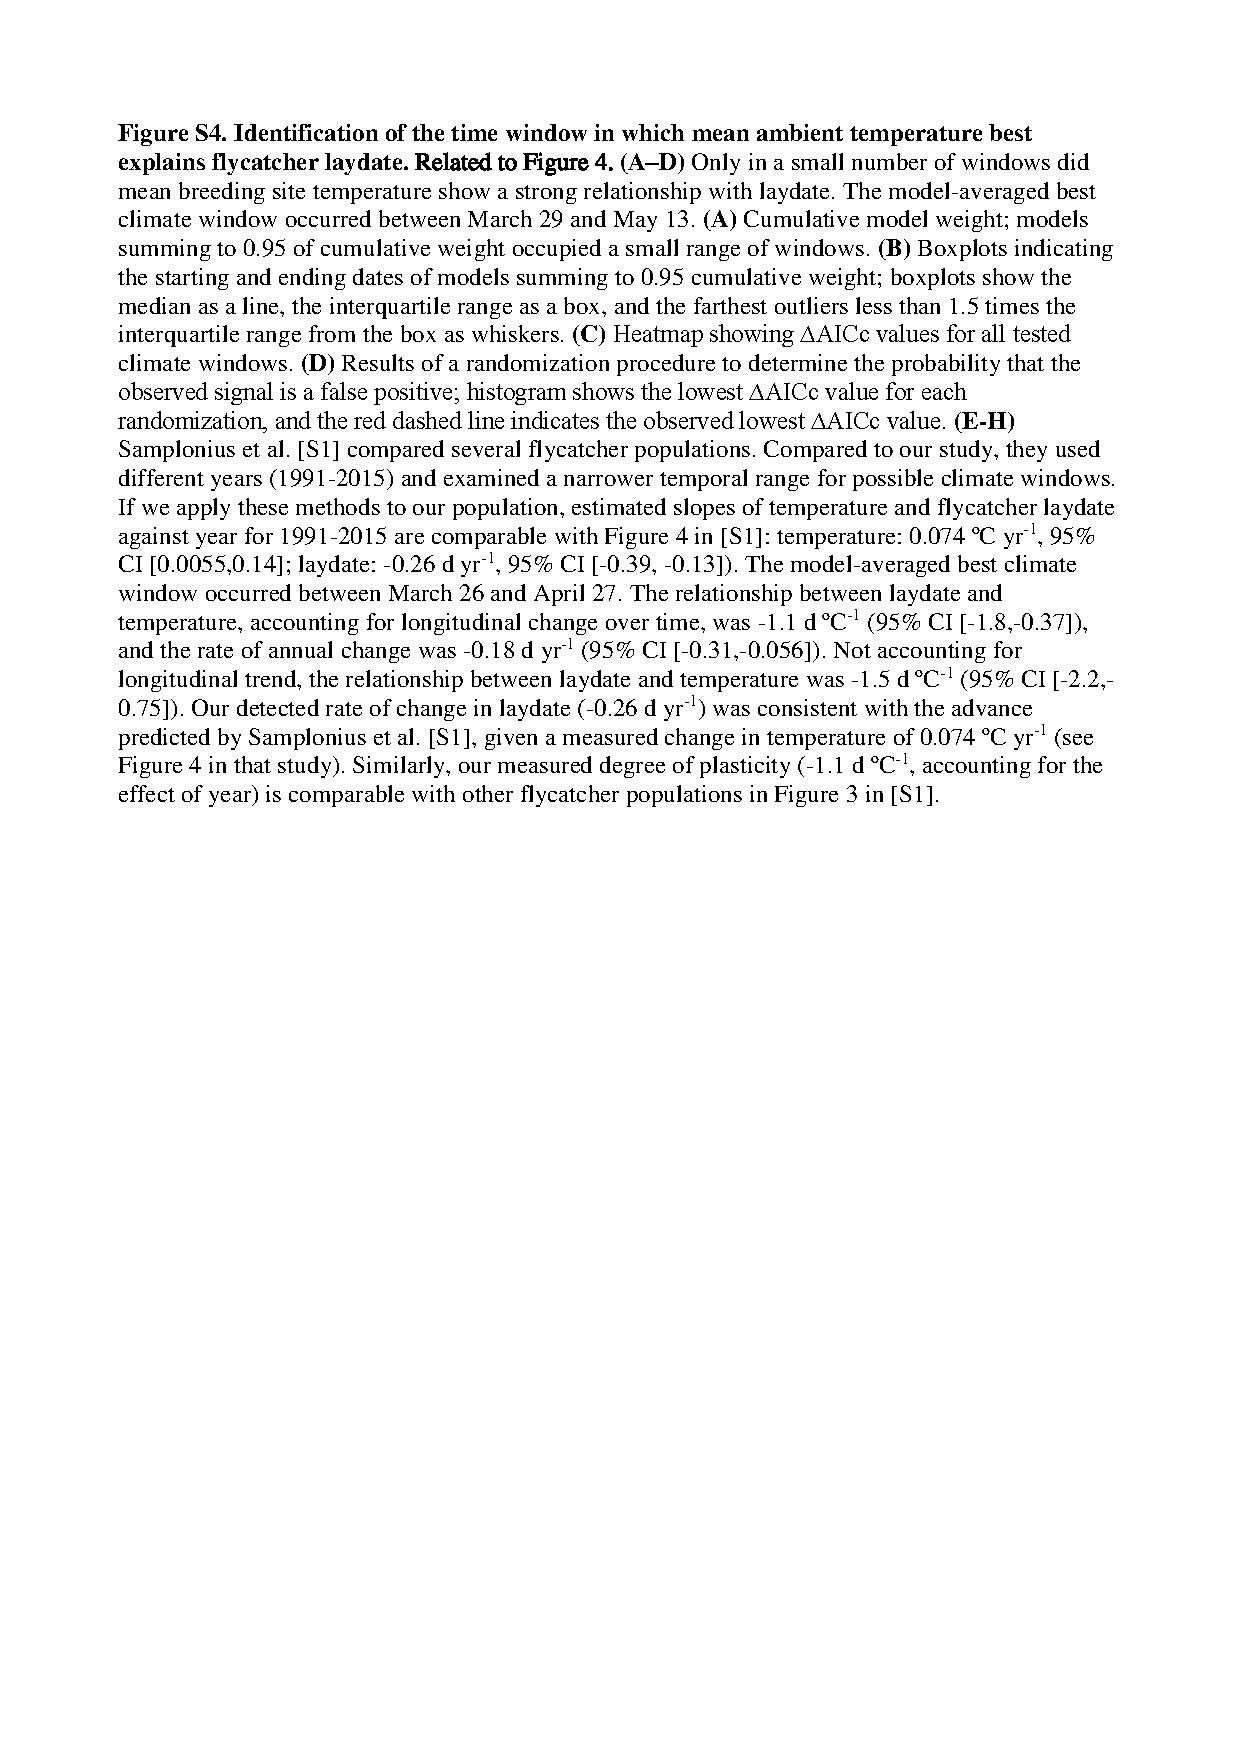
\includegraphics[width=1\linewidth]{/Users/Benjamin/Documents/Oxford/Thesis/oxforddown/pdf_chapters/pied/pied_supp_crop_Part6.pdf} \end{center} \newpage 
 \begin{center} 
\includegraphics[width=1\linewidth]{/Users/Benjamin/Documents/Oxford/Thesis/oxforddown/pdf_chapters/pied/pied_supp_crop_Part7.pdf} \end{center} \newpage

\part{A continental perspective}

\begin{savequote}
Delmore, K.,* \textbf{Van Doren, B.M.},* Conway, G.J., Curk, T.,
Garrido-Garduño, T., Germain, R.R., Hasselmann, T., Hiemer, D., van der
Jeugd, H.P., Justen, H., Lugo Ramos, J.S., Maggini, I., Phillips, R.J.,
Remisiewicz, M., Roberts, G.C.M., Sheldon, B.C., Vogl, W., and
Liedvogel, M. Formatted for \emph{Current Biology}.

\begin{scriptsize} * Equal contributions. \end{scriptsize}
\end{savequote}

\hypertarget{blackcap-geo}{%
\chapter{Versatile migratory strategies in blackcaps}\label{blackcap-geo}}

\hypertarget{summary}{%
\section{Summary}\label{summary}}

Migration is ubiquitous in the animal kingdom and may play a key role in promoting reproductive isolation \autocite{helbigSESWmigratingBlackcap1991,benschMorphologicalMolecularVariation1999,bearhopAssortativeMatingMechanism2005,irwinSiberianMigratoryDivides2005} and underpinning responses to environmental change \autocite{bertholdRapidMicroevolutionMigratory1992,plummerSupplementaryFeedingGardens2015}.
Migratory divides are contact zones between populations with different migratory phenotypes and ideal natural laboratories for studying the evolution of migration \autocite{delmoreGeneticsSeasonalMigration2016,delmoreHybridSongbirdsEmploy2014}.
The Eurasian blackcap (\emph{Sylvia atricapilla}) is a songbird that exhibits a migratory divide in central Europe between populations that migrate southwest (SW) and southeast (SE) in autumn \autocite{helbigInheritanceMigratoryDirection1991,helbigPopulationDifferentiationMigratory1992,helbigSESWmigratingBlackcap1991} and has recently established a wintering population in Britain \autocite{leachWinteringBlackcapsBritain1981,bertholdMigratoryBehaviourPopulation1988,bertholdRapidMicroevolutionMigratory1992,bearhopAssortativeMatingMechanism2005}. We tracked 108 annual migrations of 100 blackcaps captured across their range to characterize both the migratory divide and novel wintering strategy.
Blackcaps to the west and east of the divide used predominantly SW and SE directions, respectively, but close to the contact zone many individuals took intermediate (S) routes. At 14.0ºE, we documented a sharp transition (22 km) in migratory direction from SW to SE, implying a strong selection gradient across the divide.
Blackcaps wintering in Britain took northwesterly migration routes from continental European breeding grounds. They originated from a surprisingly extensive area, spanning 2000 km of the breeding range. British winterers bred in sympatry with SW-bound migrants but arrived 10 days earlier on the breeding grounds, suggesting some potential for assortative mating by timing.
Overall, our data reveal complex variation in songbird migration and suggest that selection can maintain variation in migration direction across short distances while enabling the spread of a novel strategy across a wide range.

Keywords: migration, divide, timing, songbird, speciation, assortative mating

\hypertarget{results-and-discussion}{%
\section{Results and Discussion}\label{results-and-discussion}}

Pioneering studies of blackcaps revealed that songbird migration has a genetic basis and can rapidly evolve, and these findings underlie much of our current understanding of bird migration \autocite{bertholdEvolutionaryAspectsMigratory1988,helbigInheritanceMigratoryDirection1991,bertholdRapidMicroevolutionMigratory1992,bertholdHeritabilityMigratoryActivity1994,helbigGeneticBasisMode1996,pulidoFrequencyMigrantsMigratory1996,pulidoHeritabilityTimingAutumn2001,bearhopAssortativeMatingMechanism2005,pulidoGeneticsEvolutionAvian2007,rolshausenContemporaryEvolutionReproductive2009,pulidoCurrentSelectionLower2010,muellerIdentificationGeneAssociated2011}.
Today, blackcaps may offer important insight into adaptation to environmental change, as recent population increases \autocite{ebcc/birdlife/rspb/csoTrendsCommonBirds2018} and new routes \autocite{bertholdRapidMicroevolutionMigratory1992} illustrate how this species has successfully kept pace with a changing world.
A major limitation of past studies on blackcaps has been a reliance on indirect experiments in captivity \autocite[see Chapter \ref{stonechats};][]{zunigaAbruptSwitchMigratory2016} and infrequent recaptures of ringed birds to infer phenotypes.
We sought to bridge this gap by intensively tracking blackcaps in the wild across the species' range, examining the processes shaping migratory divides and contemporary migratory change, and placing our results in an evolutionary context.

\hypertarget{tracking-blackcaps-across-a-migratory-divide}{%
\subsection{Tracking blackcaps across a migratory divide}\label{tracking-blackcaps-across-a-migratory-divide}}

Ringing and orientation studies suggest that a migratory divide exists in central Europe between blackcaps that migrate SW and SE, running north-south at 14ºE \autocite{helbigPopulationDifferentiationMigratory1992,helbigSESWmigratingBlackcap1991}. We tracked 41 annual migrations of 36 adult male blackcaps from breeding territories across the divide in Austria. To contrast behavioral variation inside and outside the divide, we also tracked blackcaps (3 F, 39 M) from breeding sites in the Netherlands (N=21), west Austria (N=6), central Germany (N=4), northern Poland (N=8), and east Austria (N=3). We expected to find a mix of strategies in the divide versus pure SW and SE directions at sites west and east of the divide, respectively.

Our tracks from central Austria clearly demonstrate the existence of a migratory divide (Figures \ref{fig:geo-plot-4}, \ref{fig:bearings-map-austria} \& \ref{fig:divide-routes-fig}). We estimated each blackcap's autumn migration direction by drawing a rhumb line between breeding and wintering areas. Migration directions varied between 130 and 288º. Intermediate (S) routes were more common (53.7\%) than SE (26.8\%) and SW (17.1\%) strategies (Figure \ref{fig:geo-plot-4}A). One individual from within the divide migrated NW to winter in Britain. Multi-year tracks revealed highly repeatable routes (Figure \ref{fig:repeat-fig}). Among-individual variation in migratory direction was considerably greater in the divide (Figure \ref{fig:var-fig-edit}), suggesting that the contact between migratory phenotypes gives rise to increased diversity of behaviors.



\begin{figure}
\includegraphics[width=1\linewidth]{_main_files/figure-latex/geo-plot-4-1} \caption{\textbf{Wintering (i.e.~non-breeding) and breeding locations of migratory blackcaps.} Wintering and breeding location estimates made with \texttt{GeoLight} shown with closed and open circles, respectively. Uncertainty in latitude estimation is indicated with vertical bars, which show estimates for sun angles higher and lower than the calibrated sun angle by 1º \autocite[following][]{hiemerFirstTracksIndividual2018}. Colors indicate SW (orange)/intermediate (green)/SE (blue)/NW (black) phenotypes, categorized by wintering location. \textbf{(A)} Blackcaps breeding within the central European migratory divide transect in Austria. \textbf{(B)} Blackcaps breeding in Austria east or west of the migratory divide. \textbf{(C)} Blackcaps breeding in the Netherlands, southern Germany, and northern Poland. \textbf{(D)} Blackcaps wintering in Britain.}\label{fig:geo-plot-4}
\end{figure}

A cline analysis using migration directions suggests that strong selection is maintaining the divide. Specifically, we examined the change in directions from western Austria (entirely SW), through the divide to eastern Austria (largely SE) (Figure \ref{fig:bearings-map-austria}; see Methods). We fit a cline through these directions to characterize its center and width. Clines maintained by selection should be narrow relative to dispersal distance, with a rapid transition between phenotypes \autocite{bartonGeneticAnalysisHybrid1993}. Our data showed this pattern: the center of the cline occurred at 14.0ºE {[}interval within two log-likelihood units: 13.8--14.2º{]}, and its width was only 22 km {[}2LL: 14--93 km{]}. This transition from SW to SE directions is very narrow compared to the average natal dispersal distance in blackcaps of 41.2 km \autocite{paradisPatternsNatalBreeding1998}.



\begin{figure}
\includegraphics[width=1\linewidth]{_main_files/figure-latex/bearings-map-austria-1} \caption{\textbf{Autumn migration directions of blackcaps in central Europe.} \textbf{(A)} Gray lines indicate migration directions of individual blackcaps, and blue lines indicate the mean direction at each capture site. In both panels, the solid vertical red line indicates the estimated cline center, and the red shading shows estimated cline width. \textbf{(B)} Autumn migration direction by breeding longitude for Austrian blackcaps, with the maximum likelihood cline plotted. Small gray dots show the directions of individual blackcaps, and large black dots represent groupings of birds treated as sites for the analysis with \texttt{hzar}, which requires grouped input data. The dotted horizontal line is 180º (due south).}\label{fig:bearings-map-austria}
\end{figure}

Our data do not allow direct identification of the source of selection, but possible processes include prezygotic selection for assortative mating and postzygotic selection reducing the fitness of hybrids. We discuss the potential for assortative mating in the next section. Helbig \autocite*{helbigInheritanceMigratoryDirection1991} selectively mated SW and SE blackcaps in captivity and observed intermediate orientations in their offspring. He argued that these hybrids would experience lower fitness through reduced survival, as they would have to cross the Alps, Mediterranean Sea, and Sahara Desert. This is a widely held hypothesis today \autocite{benschGeneticMorphologicalFeather2009,helbigInheritanceMigratoryDirection1991,irwinSiberianMigratoryDivides2005}, but our data do not necessarily support it, as a considerable number of the birds we tracked successfully took intermediate routes, survived, and returned to be recaptured. Most of these birds encountered portions of the Alps, but many did not cross the Mediterranean, in which case they never encountered this barrier or the Sahara Desert. Many of the birds that wintered in Africa navigated around the Mediterranean, and others used Italy as a land bridge (Figure \ref{fig:geo-plot-4} and \ref{fig:divide-routes-fig}).

There is one important caveat: to maximize recapture success, we exclusively tracked adult birds, which had already completed at least one migration. It is possible that some blackcaps attempt to migrate over the Mediterranean and Sahara but do not survive to adulthood. Indeed, there is a striking deficit of birds wintering in Africa around 5ºE and 15ºE (Figure \ref{fig:geo-plot-4} and \ref{fig:divide-routes-fig}; note that birds from Dutch and Polish populations did winter in these areas). This deficit would not have been present in Helbig's work because he was not tracking free-flying birds. Alvarado et al.~\autocite*{alvaradoIntegrativeTrackingMethods2014} argued similarly after failing to recover hybrids in a divide between hermit thrushes (\emph{Catharus guttatus}). At present, tracking of small songbirds is limited to archival tags not capable of transmitting daily location estimates, so we cannot address this idea further.



\begin{figure}
\includegraphics[width=1\linewidth]{_main_files/figure-latex/divide-routes-fig-1} \caption{\textbf{Full tracks of blackcaps from the migratory divide}. Tracks estimated with \texttt{FLightR}, with each track in a different color. To reduce clutter, one point is shown for each month and error bars are omitted. \texttt{FLightR} estimated some wintering locations at slightly higher latitudes than the \emph{siteEstimate} function in \texttt{GeoLight}; for example, some \texttt{FLightR} tracks that end in the southern Balkan Peninsula have \texttt{GeoLight} estimates on the northeast coast of Libya (Figure \ref{fig:geo-plot-4}A). Note that headings over short distances are sensitive to the calibration used and may not be fully trustworthy.}\label{fig:divide-routes-fig}
\end{figure}

\hypertarget{migration-timing-in-the-divide}{%
\subsection{Migration timing in the divide}\label{migration-timing-in-the-divide}}

Migration timing is an important component of the annual cycle that affects reproductive success \autocite{taylorRoleAllochronySpeciation2017,winkerOriginSpeciesHeteropatric2010} and mate selection \autocite{bearhopAssortativeMatingMechanism2005}. Assortative mating based on migratory phenotype might occur if migration timing and breeding differ consistently among phenotypes \autocite{bearhopAssortativeMatingMechanism2005}. This could result in divergence between populations with different strategies and explain the rapid transition from SW to SE phenotypes \autocite{irwinSiberianMigratoryDivides2005}. However, we found no differences in spring arrival timing between birds using SW and SE autumn strategies (effect = -0.2 days, t\textsubscript{23}=-0.046, P=0.96), nor in any other migration timing trait (Figure \ref{fig:timing-fig-combined}, Table \ref{tab:divide-timing-table}). Data from eight individual blackcaps tracked over two years suggests repeatability in timing was higher on spring migration (spring migration start: R {[}95\% CI{]}=0.85 {[}0.4,0.99{]}, end: R {[}95\% CI{]}=0.78 {[}0.36,0.96{]}; autumn migration start: R {[}95\% CI{]}=0 {[}0,0.75{]}, end: R {[}95\% CI{]}=0 {[}0,0.75{]}), albeit with considerable uncertainty in all estimates. We therefore find no evidence that the migratory divide is maintained by temporal premating isolation. Variation across the divide in other traits, including body size (approximated by tarsus length or wing length) is also absent from our dataset.



\begin{figure}
\includegraphics[width=1\linewidth]{_main_files/figure-latex/repeat-fig-1} \caption{\textbf{Repeatability of migratory phenotypes within individuals.} \textbf{(A)} Each color represents one individual tracked over two subsequent years, with solid black lines connecting location estimates for the same individual. Breeding and non-breeding sites and error bars as in Figure \ref{fig:geo-plot-4}. For the two British winterers, our repeated location estimates were very similar (59 and 92 km apart, respectively), strongly suggesting that they bred in the same area. \textbf{(B)} Migratory phenotype estimates for individuals tracked from continental Europe for two years (excluding those tagged in Britain). The dashed line is the identity line. We estimated repeatability in winter longitude as R {[}95\% CI{]}=0.99 {[}0.96,1{]} and repeatability in migration direction as R {[}95\% CI{]}=0.91 {[}0.78,1{]}. The winter location estimates for these individuals averaged 385±253 km apart in consecutive winters.}\label{fig:repeat-fig}
\end{figure}



\begin{figure}
\includegraphics[width=1\linewidth]{/Users/Benjamin/Documents/Oxford/Blackcaps/Blackcap_Geolocator_Analysis/blackcap_geo_comparative/flightr/figures_compiled/fl_all_4Feb2020_thresh1max10_b1500_nomask/draft_figures/variation_edit-01} \caption{\textbf{Variation in autumn migration direction by breeding area.} \textbf{(A)} Migration direction of tracked blackcaps caught at breeding sites across continental Europe. Each line points in the direction of autumn migration and is colored by winter region (SW=orange, intermediate=green, SE=blue, and NW (Britain)=black). Levene's test among sites with 5 or more tracked birds showed significantly higher variation in the area of the migratory divide: divide vs.~Netherlands F\textsubscript{1,61}=29.3, P\textless0.0001; divide vs.~west Austria F\textsubscript{1,45}=6.36, P=0.015; divide vs.~Poland F\textsubscript{1,47}=7.68, P=0.008 (excluding the NW migrant does not appreciably change this result). \textbf{(B)} Each dot shows the migration direction of one tracked blackcap (colored as in A). \textbf{(C)} Circular variance of autumn migration directions at each capture site, categorized by breeding region. Dot size shows the sample size at each site.}\label{fig:var-fig-edit}
\end{figure}



\begin{figure}
\includegraphics[width=1\linewidth]{_main_files/figure-latex/timing-fig-combined-1} \caption{\textbf{Blackcap migration timing}. \textbf{(A)} Timing within the migratory divide, showing model results for three timing comparisons: SW vs.~SE (left), intermediate (S) vs.~SW/SE (center), and NW vs.~SW (right). Dots give model estimate and bars 95\% confidence interval. Negative values indicate that SW or intermediate (S) groups, respectively, had earlier timing or shorter migrations. \textbf{(B)} Timing of the start of spring migration for birds tracked within the migratory divide. Points colored by wintering area, and vertical lines indicate the interquartile range of timing estimates made with \texttt{FLightR}. Curve is a loess smooth. \textbf{(C)} Boxplots showing spring migration duration by wintering area. Gray points correspond to individual tracks. \textbf{(D)} Breeding longitude vs.~spring migration timing, with NW migrants in black and other birds in green. Triangles show females and circles show males.}\label{fig:timing-fig-combined}
\end{figure}

\begin{table}[t]

\caption{\label{tab:divide-timing-table}Model results comparing migration timing in the migratory divide between SW and SE phenotypes and between intermediate (S) and SW/SE phenotypes. Log-transformed variables indicated by "(log)".}
\centering
\fontsize{9.5}{11.5}\selectfont
\begin{tabular}{l|l|r|r|r|r|r}
\hline
Contrast & Season (response) & Estimate & SE & df & t-ratio & P-value\\
\hline
SW vs. SE & Spring start & 3.14 & 7.41 & 23 & 0.42 & 0.676\\
\hline
SW vs. SE & Spring middle & 3.39 & 7.21 & 23 & 0.47 & 0.643\\
\hline
SW vs. SE & Spring end & -0.22 & 4.86 & 23 & -0.05 & 0.964\\
\hline
SW vs. SE & Autumn start & 8.33 & 5.61 & 27 & 1.49 & 0.149\\
\hline
SW vs. SE & Autumn middle & 9.23 & 6.04 & 29 & 1.53 & 0.137\\
\hline
SW vs. SE & Autumn end & 11.73 & 8.04 & 30 & 1.46 & 0.155\\
\hline
SW vs. SE & Autumn duration (log) & 0.19 & 0.70 & 25 & 0.27 & 0.791\\
\hline
SW vs. SE & Spring duration (log) & -0.80 & 0.55 & 23 & -1.44 & 0.162\\
\hline
SW vs. SE & Autumn speed (log) & -0.05 & 0.68 & 25 & -0.08 & 0.938\\
\hline
SW vs. SE & Spring speed (log) & 0.94 & 0.55 & 23 & 1.72 & 0.099\\
\hline
S vs. SW \& SE & Spring start & -14.60 & 5.49 & 23 & -2.66 & 0.014\\
\hline
S vs. SW \& SE & Spring middle & -12.97 & 5.35 & 23 & -2.42 & 0.024\\
\hline
S vs. SW \& SE & Spring end & -9.55 & 3.62 & 23 & -2.64 & 0.015\\
\hline
S vs. SW \& SE & Autumn start & -1.67 & 4.04 & 27 & -0.41 & 0.683\\
\hline
S vs. SW \& SE & Autumn middle & -4.03 & 4.20 & 29 & -0.96 & 0.345\\
\hline
S vs. SW \& SE & Autumn end & -9.70 & 5.51 & 30 & -1.76 & 0.089\\
\hline
S vs. SW \& SE & Autumn duration (log) & -0.99 & 0.53 & 25 & -1.89 & 0.070\\
\hline
S vs. SW \& SE & Spring duration (log) & 0.17 & 0.42 & 23 & 0.41 & 0.688\\
\hline
S vs. SW \& SE & Autumn speed (log) & 0.39 & 0.51 & 25 & 0.76 & 0.454\\
\hline
S vs. SW \& SE & Spring speed (log) & -0.65 & 0.42 & 23 & -1.56 & 0.133\\
\hline
\end{tabular}
\end{table}

So what is maintaining this migratory divide? One intriguing possibility is revealed by an analysis of timing that includes intermediate (S) migratory strategies. These blackcaps began spring migration on average 15 days earlier than SE and SW migrants (effect = -14.6 days, t\textsubscript{23}=-2.7, P=0.014) and arrived 10 days earlier on the breeding grounds (effect = -9.6 days, t\textsubscript{23}=-2.6, P=0.015) (Figure \ref{fig:timing-fig-combined}A, Table \ref{tab:divide-timing-table}). This pattern is apparent even if we do not categorize individuals into discrete groups (Figure \ref{fig:timing-fig-combined}B). Early spring arrival may relate to the fact that blackcaps following intermediate strategies have the shortest distances to migrate (Figure \ref{fig:mig-dist-fig}D), so cues on the wintering site may predict conditions on the breeding grounds \autocite{bothAvianPopulationConsequences2010,butlerDisproportionateEffectGlobal2003}. Importantly, early arrival may lead to assortative mating among intermediates, allowing them to exist relatively independently of pure SW and SE migrating populations within the 22 km cline. Selection against birds deviating from an immediately intermediate route (discussed previously) could limit the area where intermediates are favored to the observed cline width.

We used simulations to test if our measured distribution of arrival times would generate assortative mating among intermediate birds, comparing simulations where mate choice is dependent or independent of arrival time. The proportion of matings between intermediates was substantial and increased when we added mate selection based on timing (from 28\% with no timing to 41\% with timing), suggesting early arrival on the breeding grounds may facilitate assortative mating among intermediates, especially given their high relative abundance. Hybrid zones maintained by increased hybrid fitness are referred to as zones of bounded superiority \autocite{mooreEvaluationNarrowHybrid1977}. Additional work is needed to support this idea, including direct observations of mated pairs and their offspring in the divide. We also note that genetic differentiation across this divide is low \autocites{delmoreEvolutionaryHistoryGenomics2020}[also see][]{perez-trisHistoricalDiversificationMigration2004}{rolshausenContemporaryEvolutionReproductive2009}. However, all of the genetic work on this system has focused on allopatric populations distant from the divide \autocite{muellerIdentificationGeneAssociated2011,perez-trisHistoricalDiversificationMigration2004,rolshausenContemporaryEvolutionReproductive2009,rolshausenIndividualDifferencesMigratory2013}.

\hypertarget{origins-of-blackcaps-wintering-in-britain}{%
\subsection{Origins of blackcaps wintering in Britain}\label{origins-of-blackcaps-wintering-in-britain}}

Blackcaps wintering in the UK in increasing numbers represent a rapid and recent change in migratory behavior, illustrating the speed at which movement strategies can evolve \autocite{bertholdMigratoryBehaviourPopulation1988,leachWinteringBlackcapsBritain1981}.
Early experiments supported a genetic basis for this migratory phenotype \autocite{bertholdRapidMicroevolutionMigratory1992,helbigInheritanceNovelMigratory1994}, but its nature is still poorly understood.
Foremost is a lack of knowledge of the breeding grounds of birds wintering in Britain.
No studies have tracked the direct migrations of free-living blackcaps to understand how many adopt this novel phenotype and determine whether those breeding in Britain are also changing their behavior by adopting residency.
We fitted geolocators to blackcaps wintering in the UK and obtained 24 tracks from 22 blackcaps (12 F, 10 M), in addition to the one NW migrant tracked from our central Austrian cohort.

Blackcaps wintering in Britain originated from breeding areas in an unexpectedly broad expanse covering much of western and central Europe, remarkably extending south to latitudes occupied by the species in winter (Figure \ref{fig:geo-plot-4}D). Their autumn migrations ranged from northerly (e.g.~from Spain) to westerly (e.g.~from Poland).
This strategy enabled them to use short migration routes, on average 940±360 km; in contrast, birds tracked from central Europe flew on average 1865±717 km when they chose a southerly direction (Figure \ref{fig:mig-dist-fig}A).
Although British winterers had the shortest routes in our sample, most also bred relatively close to suitable southerly wintering areas.
To determine how far a blackcap would need to fly if it selected an alternative southerly migration route instead of a northerly route to the UK, we calculated the distance from the breeding site of each British winterer to the 10 closest wintering locations of tracked continental breeders.
In 19 out of 25 cases, the tracked route to the UK was longer than the average of the 10 possible southerly routes, often by 400-600 km (Figure \ref{fig:mig-dist-fig}C).
This suggests that migration distance is of limited importance in explaining the British overwintering strategy. The availability of reliable supplemental food in British gardens may be a key driver \autocite{plummerSupplementaryFeedingGardens2015} by positively influencing body condition and survival.

Only one of 41 individuals tracked from within the central European divide spent the winter in Britain (2.4\%, 95\% CI {[}0.13, 14{]}), and neither did any of the remaining 43 individuals tracked from elsewhere in continental Europe.
Previous studies estimated that northwest migrants comprise 6.8--25\% of individuals breeding in central Europe, based on ringing data, cage experiments, and stable isotopes \autocite{helbigPopulationDifferentiationMigratory1992,helbigSESWmigratingBlackcap1991,rolshausenContemporaryEvolutionReproductive2009,rolshausenSpringArrivalMigratory2010}.
One cage-orientation study suggested that as many as 50\% of birds breeding in the vicinity of Linz, Austria migrate northwest \autocite{helbigSESWmigratingBlackcap1991}.
Our results from free flying birds suggest these may be overestimates. Blackcaps wintering in Britain appear to breed across most of Europe at low densities, instead of occurring locally at higher densities.



\begin{figure}
\includegraphics[width=1\linewidth]{_main_files/figure-latex/mig-dist-fig-1} \caption{\textbf{Migration distances.} Colors indicate SW (orange)/intermediate (green)/SE (blue)/NW (black) phenotypes, categorized by wintering location. \textbf{(A)} Boxplots showing the distance between breeding and wintering sites for all blackcaps tracked, by deployment area. \textbf{(B)} Migration distance by breeding latitude, for all blackcaps tracked. \textbf{(C)} British winterers fly further than necessary. Values shown are the difference between the observed migration distance and the average of the distances to the 10 closest tracked individuals that wintered in traditional southerly areas, instead of in the UK. \textbf{(D)} Migration distance by wintering longitude for blackcaps tracked within the migratory divide only. Individuals with intermediate directions had the shortest migration distances.}\label{fig:mig-dist-fig}
\end{figure}

\hypertarget{timing-of-northwest-migrants}{%
\subsection{Timing of northwest migrants}\label{timing-of-northwest-migrants}}

We tested for timing differences between NW migrants (British winterers) and SW migrants that might lead to reproductive isolation.
Such timing differences have long been anticipated: Terrill and Berthold \autocite*{terrillEcophysiologicalAspectsRapid1990} predicted that differences in spring photoperiod should lead British winterers to depart and arrive c.~5 and 16 days earlier, respectively, and Bearhop et al.~\autocite*{bearhopAssortativeMatingMechanism2005} reported evidence of assortative mating by wintering latitude based on stable isotopes from claw samples.
Given that the NW phenotype appears to occur at low densities across Europe, assortative mating could be key to explaining how it is maintained in the population.

Other important factors may influence migration timing in blackcaps.
For example, protandry is common among migratory songbirds and documented in blackcaps \autocite{rainioEffectsClimateChange2007}.
In our study, females were primarily sampled from among blackcaps wintering in Britain, where they showed later spring timing than their male counterparts (Table \ref{tab:nw-timing-table}).
In addition, different parts of continental Europe experience different spring phenology.
In our dataset, blackcaps breeding further west in Europe underwent earlier spring migrations (Table \ref{tab:nw-timing-table}, Figure \ref{fig:timing-fig-combined}D).

After including breeding latitude, longitude, sex, and year as predictors to account for their effects on timing, we found that NW migrants spending the winter in Britain reached their breeding grounds earlier than SW migrants that wintered in Iberia and northwest Africa (effect = -10.3 days, t\textsubscript{44}=-4.1, P=0.0002; Table \ref{tab:nw-timing-table}, Figure \ref{fig:timing-fig-combined}).
They accomplished this by leaving the wintering grounds earlier
\autocite[effect = -6.3 days, t\textsubscript{43}=-2.5, P=0.016; compare][]{terrillEcophysiologicalAspectsRapid1990} and having shorter migration durations (ratio = 0.4x, t\textsubscript{44}=-3.3, P=0.002).
In autumn, there were no timing differences between NW and SW migrants (Figure \ref{fig:timing-fig-combined}, Table \ref{tab:nw-timing-table}).

\begin{table}[t]

\caption{\label{tab:nw-timing-table}Model results comparing migration timing of British winterers (NW migrants) to SW migrants. All models tested for timing differences between NW and SW phenotypes; other predictor variables were removed if P>0.1 and are therefore omitted from the table. Log-transformed variables indicated by  "(log)". NW and SW phenotypes differed more consistently in spring timing measures than in autumn. Likewise, protandry was evident only in spring, and breeding longitude was most strongly associated with the timing of spring migration. Breeding latitude did not show strong associations with any timing trait. Year effects were evident only in autumn, implying higher inter-annual consistency in spring.}
\centering
\fontsize{9.5}{11.5}\selectfont
\begin{tabular}{l|l|r|r|r|r|r|l}
\hline
Predictor & Season (response) & Estimate & SE & df & t-ratio & F-value & P-value\\
\hline
NW vs. SW & Spring start & -6.27 & 2.49 & 43 & -2.52 & - & 0.016\\
\hline
NW vs. SW & Spring middle & -6.83 & 2.44 & 44 & -2.80 & - & 0.008\\
\hline
NW vs. SW & Spring end & -10.28 & 2.53 & 44 & -4.06 & - & <0.001\\
\hline
NW vs. SW & Autumn start & -4.18 & 5.50 & 50 & -0.76 & - & 0.451\\
\hline
NW vs. SW & Autumn middle & 0.49 & 4.18 & 51 & 0.12 & - & 0.906\\
\hline
NW vs. SW & Autumn end & -13.04 & 6.71 & 49 & -1.94 & - & 0.058\\
\hline
NW vs. SW & Autumn duration (log) & -1.10 & 0.38 & 48 & -2.89 & - & 0.006\\
\hline
NW vs. SW & Spring duration (log) & -0.80 & 0.24 & 44 & -3.29 & - & 0.002\\
\hline
NW vs. SW & Autumn speed (log) & 0.43 & 0.44 & 48 & 0.98 & - & 0.334\\
\hline
NW vs. SW & Spring speed (log) & -0.08 & 0.23 & 44 & -0.34 & - & 0.737\\
\hline
Male vs. Female & Spring start & -9.50 & 2.88 & 43 & -3.30 & - & 0.002\\
\hline
Male vs. Female & Spring middle & -9.36 & 2.83 & 44 & -3.30 & - & 0.002\\
\hline
Male vs. Female & Spring end & -11.13 & 2.94 & 44 & -3.79 & - & <0.001\\
\hline
Male vs. Female & Autumn duration (log) & -1.00 & 0.47 & 48 & -2.10 & - & 0.041\\
\hline
Breeding longitude & Spring start & 1.22 & 0.20 & 43 & 6.02 & - & <0.001\\
\hline
Breeding longitude & Spring middle & 1.20 & 0.20 & 44 & 6.02 & - & <0.001\\
\hline
Breeding longitude & Spring end & 1.16 & 0.21 & 44 & 5.59 & - & <0.001\\
\hline
Breeding longitude & Autumn end & 0.86 & 0.39 & 49 & 2.17 & - & 0.035\\
\hline
Breeding longitude & Autumn duration (log) & 0.10 & 0.03 & 48 & 3.32 & - & 0.002\\
\hline
Breeding longitude & Autumn speed (log) & -0.07 & 0.03 & 48 & -2.79 & - & 0.007\\
\hline
Breeding latitude & Autumn end & -1.62 & 0.91 & 49 & -1.79 & - & 0.08\\
\hline
Breeding latitude & Autumn speed (log) & 0.13 & 0.07 & 48 & 1.93 & - & 0.06\\
\hline
Year (F-test) & Autumn start & - & - & - & - & 6.44 & 0.001\\
\hline
Year (F-test) & Autumn middle & - & - & - & - & 6.94 & 0.001\\
\hline
Year (F-test) & Autumn end & - & - & - & - & 2.25 & 0.094\\
\hline
Year (F-test) & Autumn duration (log) & - & - & - & - & 2.85 & 0.047\\
\hline
Year (F-test) & Autumn speed (log) & - & - & - & - & 3.13 & 0.034\\
\hline
\end{tabular}
\end{table}

Our data support the hypothesis that differences in arrival timing may contribute to reproductive isolation among blackcaps wintering in Britain, likely due to a combination of differing photoperiodic cues and shorter migrations \autocite{terrillEcophysiologicalAspectsRapid1990}.
Early-arriving individuals from Britain may experience fewer hazards during faster journeys, they may be in better condition due to supplemental food in British gardens \autocite{bearhopAssortativeMatingMechanism2005,plummerSupplementaryFeedingGardens2015}, and they may be able to use local weather cues to judge the suitability of their continental breeding areas.
In turn, these individuals may be able to secure higher quality territories.
However, it is unclear whether the magnitude of the timing difference (10 days) could result in effective reproductive isolation.
Rolshausen et al.~\autocite*{rolshausenSpringArrivalMigratory2010} modeled assortative mating based on a timing difference of 10 days and a relative abundance of NW migrants of 1 out of 13 breeding individuals, concluding that NW migrants had a 28\% chance of mating assortatively.
Although we only tracked one NW migrant from within the migratory divide and therefore cannot capture the distribution of arrival dates in this particular breeding population, our similar average timing difference and lower relative abundance of NW migrants corroborate their conclusion of weak evidence for effective isolation solely based on timing.
However, differences in body condition or microhabitat selection by migratory phenotype \autocite{rolshausenSpringArrivalMigratory2010} could still contribute to reproductive isolation.

\hypertarget{conclusion}{%
\subsection{Conclusion}\label{conclusion}}

We find considerable variation in blackcap migratory behavior across the central European migratory divide and diverse breeding origins for blackcaps exhibiting the novel British overwintering strategy. A narrow cline in migration direction across the divide suggests that selection on migratory strategy is strong. Assortative mating among birds orienting immediately south and selection against those deviating from this direction may help maintain this narrow cline. British winterers arrived on continental breeding grounds earlier than migrants from Mediterranean wintering areas, but the difference in timing may be insufficient to drive assortative mating. Accurately characterizing the migrations of individual blackcaps reveals fascinating variability in the migratory behavior of this species, paving the way for targeted studies of the genetic basis of migration and adaptation to global change.

\hypertarget{methods}{%
\section{Methods}\label{methods}}

\hypertarget{geolocator-application-and-retrieval}{%
\subsection{Geolocator application and retrieval}\label{geolocator-application-and-retrieval}}

From 2016--2019, we deployed 806 archival light-level geolocators on breeding blackcaps in Austria (N=376, May--June), Germany (N=57, May--August), the Netherlands (N=189, May--July), and Poland (N=53, April--May and August), and on wintering Blackcaps in the United Kingdom (N=131, January--March) (Table \ref{tab:capture-recapture-table}). In Austria, we focused our sampling on the anticipated location of the migratory divide, where blackcaps with eastern and western migratory routes meet, and including populations that prior studies suggested contained NW migrants \autocite{helbigPopulationDifferentiationMigratory1992,helbigSESWmigratingBlackcap1991}.

We captured birds using mist nets and tape luring with audio recordings of the male blackcap territorial song. In the UK, we captured birds attending feeding stations in suburban gardens with mist nets and potter traps. We used leg-loop harnesses \autocite{rappoleNewHarnessDesign1991} made from elastic, viton, or nylon to attach geolocators. Tags were various models manufactured by Migrate Technology Ltd (see Table \ref{tab:capture-recapture-table}). Overall, we retrieved 117 devices, of which 108 contained data from at least one complete migration. We concurrently marked control cohorts in the United Kingdom and the Netherlands (see Table \ref{tab:capture-recapture-table}). Return rates did not significantly differ between control and tagged birds (Fisher's exact test, UK: P=0.25; Netherlands: P=1).

\begin{table}[t]

\caption{\label{tab:capture-recapture-table}Geolocator deployment summary. All devices manufactured by Migrate Technology Ltd. Nylon material refers to 1 mm nylon braid for harnesses, viton refers to 0.6 mm viton rubber cord, and elastic refers to 0.7-0.8 mm stretch elastic. "Deploy", "Return", and "Recover" respectively refer to the number of devices deployed, the number of birds that were observed to have returned with devices, and the number of devices ultimately recovered from returning birds.}
\centering
\fontsize{9.5}{11.5}\selectfont
\begin{tabular}{l|l|l|l|l|l|>{\raggedright\arraybackslash}p{9em}}
\hline
Region & Year & Deploy & Return & Recover & Material & Device\\
\hline
Austria & 2016 & 202 & 24 (5 viton) & 24 & nylon, viton & P65Z1top2end-11\\
\hline
Austria & 2017 & 159 & 28 & 27 & nylon & P50Z11-11\\
\hline
Austria & 2018 & 15 & 4 & 3 & nylon & P65Z1top1-11\\
\hline
Netherlands & 2016 & 61 & 5 & 5 & nylon & P50B1-11\\
\hline
Netherlands & 2017 & 61 & 8 & 7 & nylon & P50B1-11\\
\hline
Netherlands & 2018 & 67 & 14 & 13 & elastic & P30Z11-7-DIP-NOT; P65B1-7-NOT\\
\hline
Poland & 2015 & 12 & 1 & 1 & nylon & W30Z11-DIP-NOT; W65B1-DIP NOT\\
\hline
Poland & 2016 & 9 & 1 & 1 & nylon & W30Z11-DIP-NOT; W65B1-DIP NOT\\
\hline
Poland & 2017 & 12 & 4 & 4 & nylon & W65B1-DIP NOT; W30Z11-DIP-NOT\\
\hline
Poland & 2018 & 20 & 4 & 3 & nylon & W65B1-DIP NOT; W30Z11-DIP-NOT\\
\hline
S Germany & 2018 & 57 & 7 & 5 & elastic & P30Z11-7-DIP-NOT; P65B1-7-NOT\\
\hline
UK & 2016-17 & 36 & 8 & 6 & elastic & P50Z11-11-NOT\\
\hline
UK & 2017-18 & 48 & 11 & 7 & elastic & P50Z11-7-DIP-NOT\\
\hline
UK & 2018-19 & 47 & 15 & 11 & elastic & P50Z11-11-NOT\\
\hline
\end{tabular}
\end{table}

\hypertarget{analysis-of-light-data}{%
\subsection{Analysis of light data}\label{analysis-of-light-data}}

We first used the \emph{preprocessLight} function in the \texttt{TwGeos} \autocite{wotherspoonTwGeosBasicData2016} R package to define twilight events. We used a light threshold of 1.5 lux because blackcaps often occupy darker understory and mid-story habitats \autocite{rakhimberdievComparingInferencesSolar2016}. To maximize repeatability, we minimized manual processing. We manually removed only obviously erroneous twilights, focusing on calibration periods. After manual processing, we used the \emph{twilightEdit} function in \texttt{TwGeos} to perform additional automated editing and deletion of erroneous twilights. We used the following settings in \emph{twilightEdit}: window = 4, outlier.mins = 30, and stationary.mins = 15. In the case of two devices with substantial shading of the light sensor, \emph{twilightEdit} removed too many twilights to use in downstream analysis; in this case, we used only manually processed twilight times.

We used \texttt{FLightR} \autocite{rakhimberdievFLightRPackageReconstructing2017,rakhimberdievHiddenMarkovModel2015} to determine migration timing. \texttt{FLightR} uses the slope of the light curve around twilight to estimate locations and is therefore sensitive to data quality. In our dataset, several devices experienced substantial shading due to mantle feathers covering the light sensor, especially after the summer molt of body feathers. Geolocators with shorter ``light pipes'' (``-7'' models, see Table \ref{tab:capture-recapture-table}) or with the light sensor on the body of the device itself (deployed in Poland, see Table \ref{tab:capture-recapture-table}) were prone to this issue, whereas devices with a light sensor at the end of a 11-mm ``light stalk'' (``-11'' models) rarely experienced shading. We performed an automated step to remove highly shaded light curves. For each twilight event, we took the mean of all ``log.light'' values returned by \texttt{FLightR} and removed twilights with values less than 1. We removed no more than 10\% of twilights with this method; if more than 10\% of twilights were heavily shaded, we removed the worst 10\%. This approach improved performance for most individuals with light to moderate shading of the light sensor, but we were unable to obtain \texttt{FLightR} tracks for 6 heavily shaded devices. These were excluded from the \texttt{FLightR} timing analysis.

To identify birds' migration destinations (i.e.~breeding or wintering sites, depending on the season of deployment), we used the R package \texttt{GeoLight} \autocite{lisovskiGeoLightProcessingAnalysing2012}. \texttt{GeoLight} contains a function \emph{siteEstimate} for estimating a bird's location during a given time period, specifically designed for blackcaps and other birds for which shading of the light sensor can be a problem \autocite{hiemerFirstTracksIndividual2018}. We succeeded in using \emph{siteEstimate} to obtain location estimates for all birds, including those for which \texttt{FLightR} had failed. For devices deployed in summer, we used twilights from 15 December to 15 January to estimate wintering locations. For devices deployed in winter, we used twilights from 1 June to 1 August to estimate summer breeding locations. In both cases, we set these time periods in mid-winter and mid-summer, when they are least likely to overlap with spring and autumn movements. We used the same time window for all birds to obtain comparable locations across individuals.

Both \texttt{GeoLight} and \texttt{FLightR} require that users define calibration periods during which the bird was stationary in a known location. We set calibration periods by visually inspecting plots of the log of observed versus expected light slopes for the deployment site over time (\emph{plot\_slopes\_by\_location} function in \texttt{FLightR}). When a bird moves away from the deployment site, the observed and expected slopes visually diverge \autocite{lisovskiLightlevelGeolocatorAnalyses2020}. For some individuals, visual resighting data were available after deployment and before recapture to aid calibration. After running \texttt{FLightR}, we refined calibration periods if the analysis suggested that movement had occurred during calibration periods. Some devices had insufficient calibration periods, if, for example, the bird departed shortly after tagging and the device stopped recording before the return migration. In these cases, and cases where the resulting track showed clear signatures of poor calibration (e.g.~latitudinal drift during stationary periods or widely varying location estimates), we used a global calibration made from the combined data of all devices. For this global calibration, we used a linear model to estimate the overall mean calibration slope, accounting for the magnitude of shading to the light sensor. We did not include devices that lacked light pipes or light stalks, which made the light data qualitatively different from those collected by the other devices.

In \texttt{GeoLight}, we used the same calibration periods as for \texttt{FlightR}, with one additional refining step: we used \emph{siteEstimate} to estimate the location of deployment and compared the result to the actual deployment location; if a lower or higher sun angle (±0.25º increments) resulted in a more accurate estimate of the deployment site, we used the adjusted sun angle instead.

We defined the \texttt{FLightR} model search grid between 10ºS and 65ºN latitude and 20ºW and 52ºE longitude. We chose these settings after visually inspecting light data with the \emph{thresholdPath} function in the R package \texttt{SGAT} \autocite{lisovskiGeoLightProcessingAnalysing2012,sumnerBayesianEstimationAnimal2009} to confirm that no tracks were likely to occur outside of this area.
\texttt{FLightR} contains a prior for the decision to move, which has a default of 0.05. We adjusted this setting outside of the migration season (i.e.~from Dec 15--Mar 1 and May 15--Aug 15) to a value of 0.001. For the final run of each individual, we ran the particle filter with the recommended 1 million particles.

\hypertarget{migratory-phenotypes}{%
\subsection{Migratory phenotypes}\label{migratory-phenotypes}}

For comparative analyses of migratory phenotypes, we used both (1) winter longitude and (2) autumn migration direction. We estimated the bird's direction on autumn migration as the rhumb line connecting breeding and wintering sites \autocite[\emph{bearingRhumb} in R package \texttt{geosphere},][]{hijmansGeosphereSphericalTrigonometry2017}. We used this simplified representation of the route for calculating migration direction because geolocator tracks over short distances are sensitive to bias caused by imperfect calibration, especially close to an equinox.

In geolocation analyses of bird migration, longitude can generally be estimated with greater precision than latitude \autocite{lisovskiGeolocationLightAccuracy2012,ekstromAdvanceGeolocationLight2004,fudickarTrackingMigratorySongbirds2012}. Latitude estimates are derived from daylengths, which can be affected by shading and are unreliable around the spring and autumn equinoxes. We compared destination longitudes estimated with \texttt{GeoLight} (\emph{siteEstimate}) to estimates derived from \texttt{FLightR}. The two methods were highly correlated (\(\rho\)=0.99), affirming destination longitude as a reliable measure of migratory phenotype that is insensitive to the choice of analysis method. Destination latitude showed a slightly lower correlation between the two methods (\(\rho\)=0.82).

On 8 occasions, we were able to track the same individual for two subsequent years (5 from the migratory divide, 1 from the Netherlands, and 2 from Britain). From these data, we estimated individual repeatability using the R package \texttt{rptR} \autocite{stoffelRptRRepeatabilityEstimation2017} as the proportion of total variation explained by bird identity, where the total includes both variation from bird identity and among-year variation among birds.

We assigned individuals to four categories based on wintering location. For birds wintering north of 37.5ºN, we considered those west of 5ºE to be southwest (SW) migrants, those east of 20ºE to be southeast (SE) migrants, and those between 5-20ºE to have intermediate southerly (S) routes. For birds wintering south of 37.5ºN, we used a cutoff of 0º to distinguish SW from S because these longer routes require less of a westerly component to reach the same longitude.

We used Levene's test to compare variances (\emph{leveneTest} R function in the \texttt{car} package) to determine whether the distribution of autumn migration directions differed among breeding sites. We controlled for multiple testing by applying a false discovery rate correction using the \emph{p.adjust} R function.

\hypertarget{timing}{%
\subsection{Timing}\label{timing}}

We calculated migration timing using the \emph{find.times.distribution} function in \texttt{FLightR}. To use this function, the user defines a spatial area, and the function reports the time at which the bird was likely to have crossed into and out of that area. For each individual, we used the shortest-distance route (i.e.~a great circle route) between summer and winter areas to aid in defining migration progress. Specifically, we calculated paths perpendicular to the shortest-distance route at 30\%, 50\%, and 70\% of the way between summer and winter locations, and we used \emph{find.times.distribution} to determine when on migration the bird crossed these thresholds. We chose values of 30 and 70\% because we found using values closer to the endpoints of the journey (e.g.~15\%/85\%) caused a higher proportion of calculations to fail, which typically occurs when the bird does not transit cleanly across the threshold. Close to summer and winter sites, local movements and geolocation uncertainty over time may lead to the modeled bird's path approaching the threshold more than twice per year. We treated these thresholds (30\%, 50\%, 70\%) as representing early, middle, and late stages of the migratory journey, and we considered a bird to have reached each point at the 0.50 quantile time returned by \emph{find.times.distribution.} As a measure of migration duration, we calculated the number of days it took each bird to travel from early (30\%) to late (70\%) migration stages, setting the value to one if it was estimated as less than one day. We calculated the speed of migration by dividing migration distance by duration. Because timing estimates of north-south movements can be inaccurate near the equinox, we did not retain timing estimates of movements taking place within 7 days of an equinox along a route within 15º of due north or south.

We validated \texttt{FLightR} timing estimates using simple longitude coordinate output from \texttt{GeoLight} (\emph{crds} function), which we used to derive alternative measures of migration timing across an east-west axis. With this method, we considered a bird to be halfway through its migration when its estimated longitude was closer to the longitude of its destination than its origin. We defined the start of migration as the time when a bird crossed a threshold from its starting longitude and did not return. Our threshold was defined as 10\% of the difference between origin longitude and destination longitude. We defined the end of migration as the point when a bird crossed to within 10\% of its destination longitude. We expected migration timing estimated from longitude data to be most comparable to \texttt{FLightR} estimates for birds that primarily used east-west routes. For birds that primarily moved along a north-south axis, the component of movement across longitudes is small relative to the component across latitudes. Therefore, we excluded birds with strongly southerly migration directions (150º--210º) from this validation. The timing of spring migration was consistent across methods (all Spearman \(\rho\)\textgreater0.78). In autumn, \(\rho\) ranged from 0.61 to 0.76.

We constructed linear models to compare the timing of migration for three different comparisons. For individuals tracked within the Austrian migratory divide, we tested for differences (1) between SW and SE parental phenotypes, and (2) between intermediate (S) and parental (SW/SE) phenotypes. Finally, we (3) tested for differences between NW (i.e.~UK) and SW phenotypes. In all cases, we tested fixed effects of wintering area (NW/SW/S/SE) and year. We attempted to fit a random effect of bird identity, but our sample size of repeat tracks (N=8) was insufficient to estimate a variance component of bird identity, resulting in singular fits. Therefore, for birds with repeat tracks we randomly chose one track to include in the timing analysis, so that only one data point per individual was included for each timing measure. For comparison 3 (NW vs.~SW), we also included effects of sex and breeding latitude and longitude. These effects were not relevant for comparisons 1 and 2 because all birds were tracked from a single breeding area (the divide zone), and all tracked birds were males. We used the R package \texttt{emmeans} \autocite{lenthEmmeansEstimatedMarginal2019} to construct the proper contrasts for comparisons 1 and 2. To maximize the precision of our estimates given a limited sample size, we removed terms with P-values greater than 0.10. For migration speed and duration, which had right-skewed distributions, we log-transformed the response variable before fitting the model.

We used simulations to investigate whether our measured arrival timing differences in the migratory divide among SW, SE, and S (intermediate) phenotypes could lead to substantial assortative mating. In each simulation, we used the observed relative abundances of S, SW, and S phenotypes in the divide to draw a random sample of birds of equal number, following a multinomial distribution. Then, we used density curves fit to the original data to draw a sample of arrival dates for each phenotype group. Finally, for each individual, we selected a random mate based on the proportions of individuals present five days after its simulated arrival date. We used this delay because pair formation occurs within days of arrival \autocite{bairleinUeberBiologieSuedwestdeutschen1978} and females tend to arrive later than males. We repeated this simulation 1000 times and extracted the proportion of pairings that occurred between individuals that had taken intermediate routes.

\hypertarget{routes}{%
\subsection{Routes}\label{routes}}

We used route output from \texttt{FLightR}. For tags that stopped in late winter or close to the spring equinox, track estimates could be unreliable. In these cases (n=16), we ignored location estimates for dates after 1 January if the tag stopped operation within three weeks of the spring equinox.

\hypertarget{cline-analysis}{%
\subsection{Cline analysis}\label{cline-analysis}}

We used the R package \texttt{hzar} \autocite{derryberryHzarHybridZone2014} to estimate the location and width of the cline marking the transition from westerly to easterly migratory directions in the migratory divide. We used code from the supplementary material of Derryberry et al.~\autocite*{derryberryHzarHybridZone2014} as the basis for the analysis. Because \texttt{hzar} assumes that data come from a one-dimensional transect (in our case, an east-west transect), we limited the sites we included to the narrow range of latitudes within Austria. The analysis requires input data in the form of sites (not individuals), so we grouped individuals in the following way: we treated individuals as belonging to the same site group if their breeding territories were within 0.2 degrees of longitude, setting a maximum group size of 5 unless doing so would create an individual without a group. In this way, we assigned individuals to similarly-sized groups based on the longitude of their breeding site in Austria.

\hypertarget{author-contributions}{%
\subsection{Author contributions}\label{author-contributions}}

Conceptualization: KD, BMVD, BCS, ML; Methodology: KD, BMVD; Formal Analysis: KD, BMVD; Fieldwork: KD, BMVD, TC, TGG, RRG, TH, DH, HJ, IM, JSLR, BSM, RJP, MR, GCMR, HPJ, WV, ML; Writing --Original Draft: BMVD with input from KD and ML; Writing --Review \& Editing: KD, BMVD, GJC, TC, TGG, RRG, JSLR, IM, BSM, MR, BCS, HPJ, WV, ML; Visualization: BMVD; Supervision: GJC, MR, HPJ, BCS, ML; Project Administration: WV, IM, HPJ, GJC, MR, ML; Funding Acquisition: BMVD, MR, HPJ, ML.

\hypertarget{declaration-of-interests}{%
\subsection{Declaration of Interests}\label{declaration-of-interests}}

The authors declare no competing interests.

\hypertarget{acknowledgements}{%
\subsection{Acknowledgements}\label{acknowledgements}}

For fieldwork assistance and logistical support, we thank Mayra Zamora, Gillian Durieux, Karen Bascon Cardozo, Andrea Bours, Shraddha Lall, Lisa Kettemer, Vasiliki Tsapalou, Josef Hemetsberger, Hans Winkler, Hemma Gressel, Alwin Schönenberger, Gerd Spreitzer, OSR Dir. Reinhold Petz, Mikkel Willemoes, Anne Hloch, Clara Leutgeb, Lisa Rosenich, Marius Adrion, Simon Kofler, Wolfgang Fiedler, Sally Amos, Jon Avon, Jake Bailey, Penny Barret, Stuart Bearhop, Rob and Liz Boon, Stuart Brown, Malcolm Burgess, Emily Cuff, Kate Dalziel, Ian Duncan, Rachel Durham, Phil Evans, Sheila Evans, Kate Fox, Roger Francis, Lyn Gammage, Gill Garrett, Sheila Gowers and Paul Ensom, Mark Grantham, Jodie Mae Henderson, John and Jane Holmes, Emma Inzani, Brian Isles, Michael and Helen Johnson, Ben Porter, Mel Mason, Irene McGregor, Keith McMahon, Nicole Milligan, Dee and Jonnie Reeves, Fiona Roberts, Dr ET Roberts, Gary Samways, Ash Sendell-Price, Ana Shapiro, Anna Smith, Dave Stoddard, Esmé Tackley, John Webber, Kester Wilson, Penny Witcombe, and other contributors, ringers, and homeowners. Special thanks to Glynne Evans for generous support and guidance. We thank Krzysztof Stępniewski, Katarzyna Stępniewska, Michał Redlisiak, and the Operation Baltic team of citizen scientists at Bukowo, Poland; Tijs van den Berg, Henri Bouwmeester, Ruud Foppen, Arend Timmerman, Morrison Pot and Hans Vlottes; James Fox and Migrate Technology Ltd for reliable geolocators and excellent technical support; and Eldar Rakhimberdiev and Simeon Lisovski for invaluable technical insights.

This work was supported through funding from the Max Planck Society (MPRG grant to ML), the Natural Sciences and Engineering Research Council (NSERC PDF, to KED), the Marshall Aid Commemoration Commission (to BMVD), the American Ornithological Society (Mewaldt-King Research Award, to BMVD), the Society for the Study of Evolution (Rosemary Grant Award, to BMVD), the Frank M. Chapman Memorial Fund (to BMVD), the British Trust for Ornithology (to BMVD), 3V-Fonds from the Royal Netherlands Academy of Sciences and from NIOO-KNAW (both to HJ), and Special Research Facility grants (SPUB) of the Polish Ministry of Science and Higher Education to the Bird Migration Research Station, University of Gdańsk (to MR). See Supplementary Material for a list of ethical approvals and permits.

In Austria, fieldwork was approved by the institutional ethics and animal welfare committee and the national authority (GZ 68.205/0048-WF/V/3b/2016) according to §§ 26ff. of Animal Experiments Act, Tierversuchsgesetz 2012 -- TVG 2012. Permit numbers: GZ BMWFW-68.205/0048-WF/V/3b/2016 and BMWFW-68.205/0139-WF/V/3b/2016 (AT), UID: ATU36801500, MA22-24411/2016 (Wien): BHBR-I-7100.00-69/2016-13 (VA), ABT13-53V-10/1998-42 (Steiermark), 205-05RI/549/58/7-2016 (Salzburg), N-2016-197947/8-Pin (Oberösterreich), VL3-NS-3068/2016 /005/2016) (Kärnten, Villach), SV19-ALL-938/2016 (004/2016) (Kärnten, St Veit), SP3-NS-2823/2016 (007/2016) (Kärnten, Spittal), HE3-NS-1280/2016 (005/2016) (Kärnten, Hermagor), FE3-NS-2127/2016 (006/2016) (Kärnten, Feldkirchen), 5/N.AB-10120-8-2016 (Burgenland), RU5-BE-286/011-2016 (Niederösterreich). In the UK, geolocator deployments were approved by the University of Oxford Animal Welfare Ethical Review Body. Work was conducted under licenses from the British Trust for Ornithology, approved by the Special Methods Technical Panel. In Poland, work was approved by the General Directorate for Environmental Protection within the permit to capture and ring wild birds (DZP-WG.6401.03.36.2015.km, DZP-WG.6401.03.98.2016.km, DZP-WG.6401.03.97.2017.jro, DZP-WG.6401.03.2.2018.jro). In Germany, the permit was issued by the Regierung von Mittelfranken, Bavaria. Permit number: 54-2532.1-13/14. In the Netherlands, the permit was issued by the Centrale Commissie Dierproeven. Permit number: AVD801002016519 valid 27-6-2016 through 31-5-2021.

\clearpage \printbibliography[segment=  herefsection,heading=subbibliography]

\begin{savequote}
\textbf{Van Doren, B.M.} and Horton, K.G. (2018). A continental system
for forecasting bird migration. \emph{Science} 361, 1115--1118.

Reprinted with permission from AAAS.
\end{savequote}

\hypertarget{forecast}{
\chapter[A continental system for forecasting bird migration]{A continental system for\\forecasting bird migration}\label{forecast}}
\chaptermark{Forecasting bird migration}

\newpage

\begin{center} \makebox[\linewidth][c]{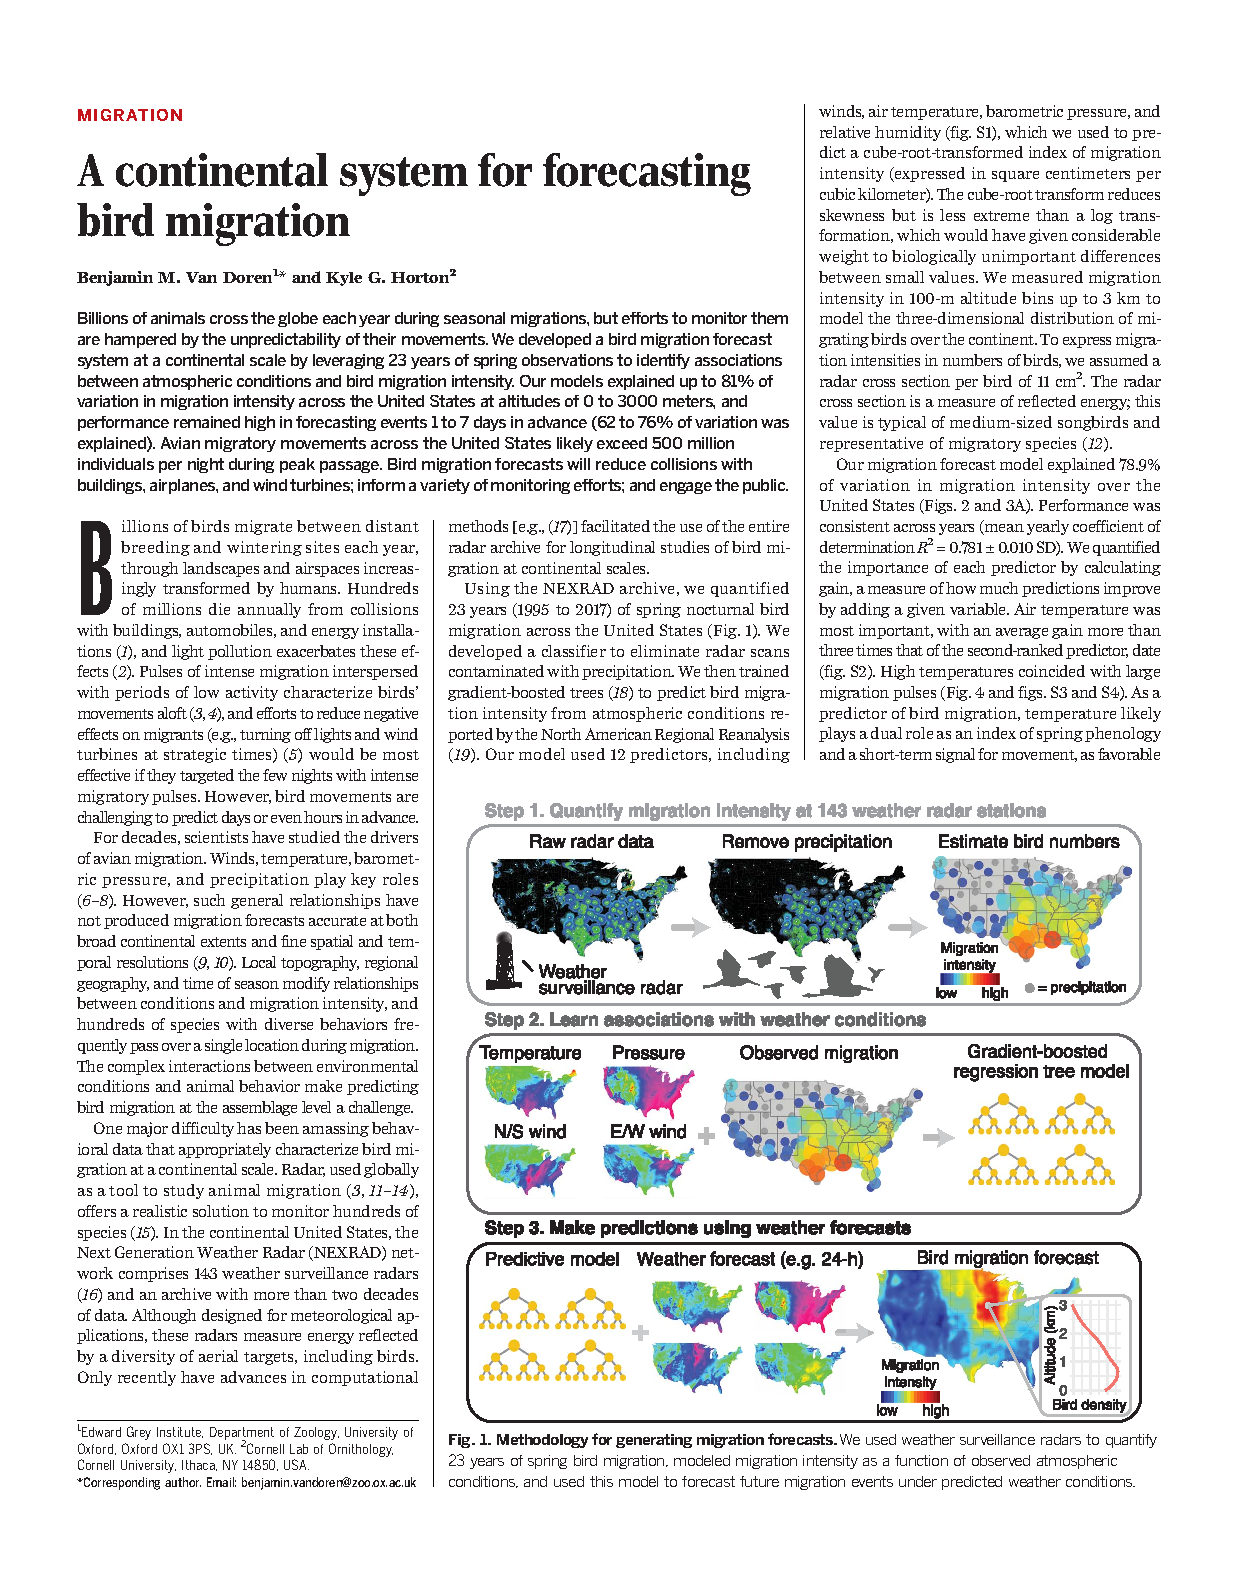
\includegraphics[width=1.2\linewidth]{/Users/Benjamin/Documents/Oxford/Thesis/oxforddown/pdf_chapters/forecast/forecast_crop_Part1.pdf}} \end{center} \newpage 
 \begin{center} \makebox[\linewidth][c]{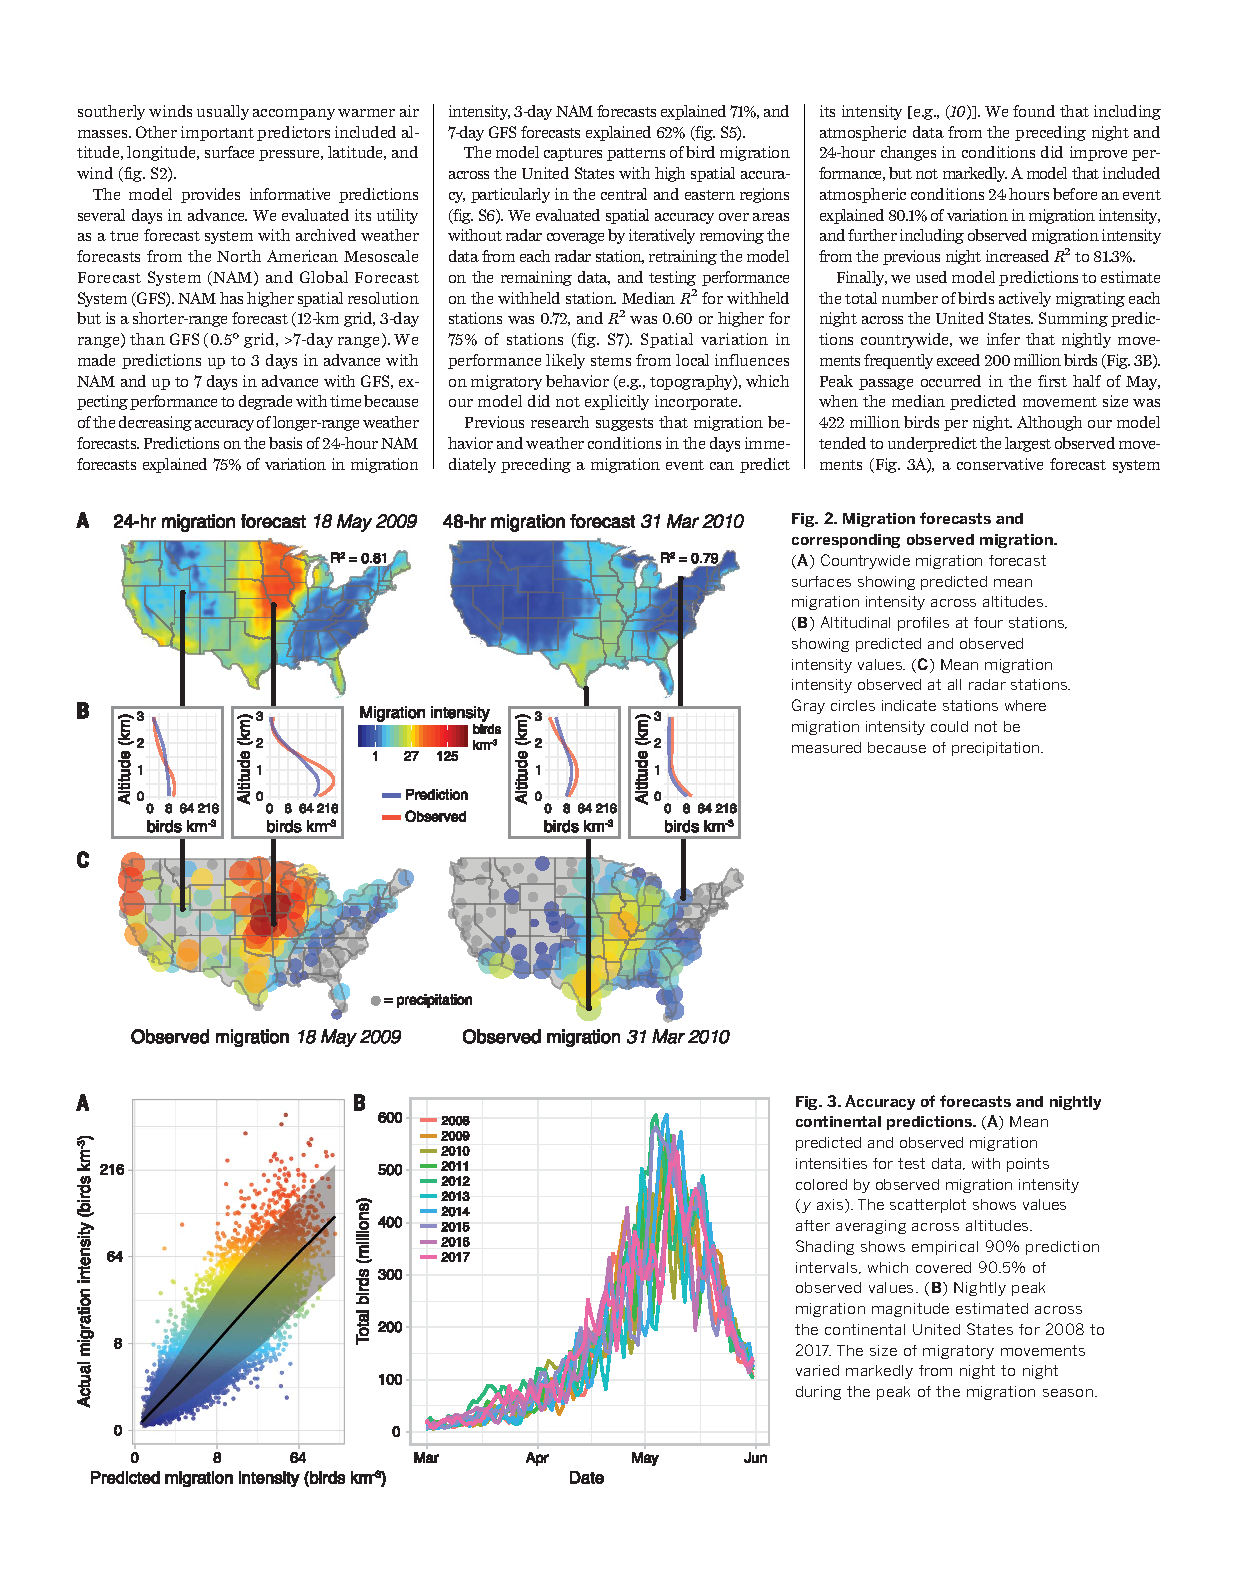
\includegraphics[width=1.2\linewidth]{/Users/Benjamin/Documents/Oxford/Thesis/oxforddown/pdf_chapters/forecast/forecast_crop_Part2.pdf}} \end{center} \newpage 
 \begin{center} \makebox[\linewidth][c]{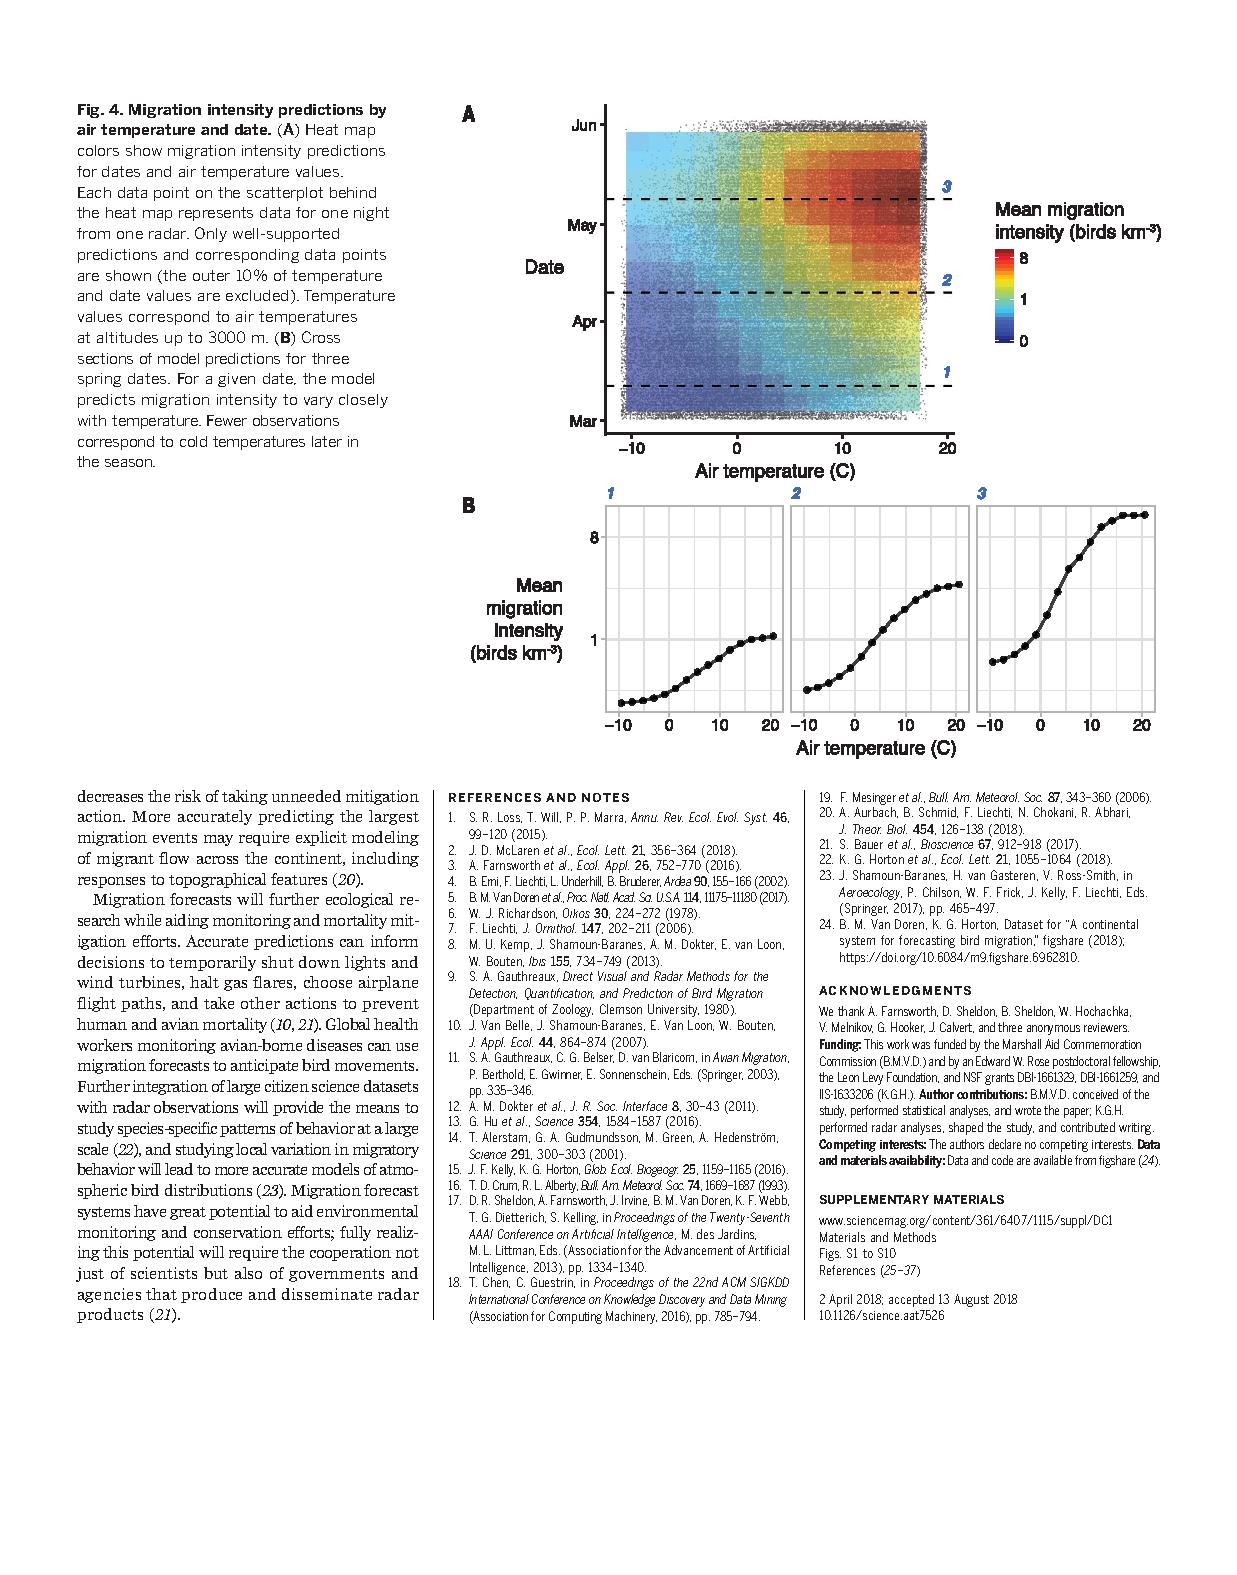
\includegraphics[width=1.2\linewidth]{/Users/Benjamin/Documents/Oxford/Thesis/oxforddown/pdf_chapters/forecast/forecast_crop_Part3.pdf}} \end{center} \newpage

\begin{center} \makebox[\linewidth][c]{
\includegraphics[width=1.1\linewidth]{/Users/Benjamin/Documents/Oxford/Thesis/oxforddown/pdf_chapters/forecast/forecast_supp_crop_Part01.pdf}} \end{center} \newpage 
 \begin{center} \makebox[\linewidth][c]{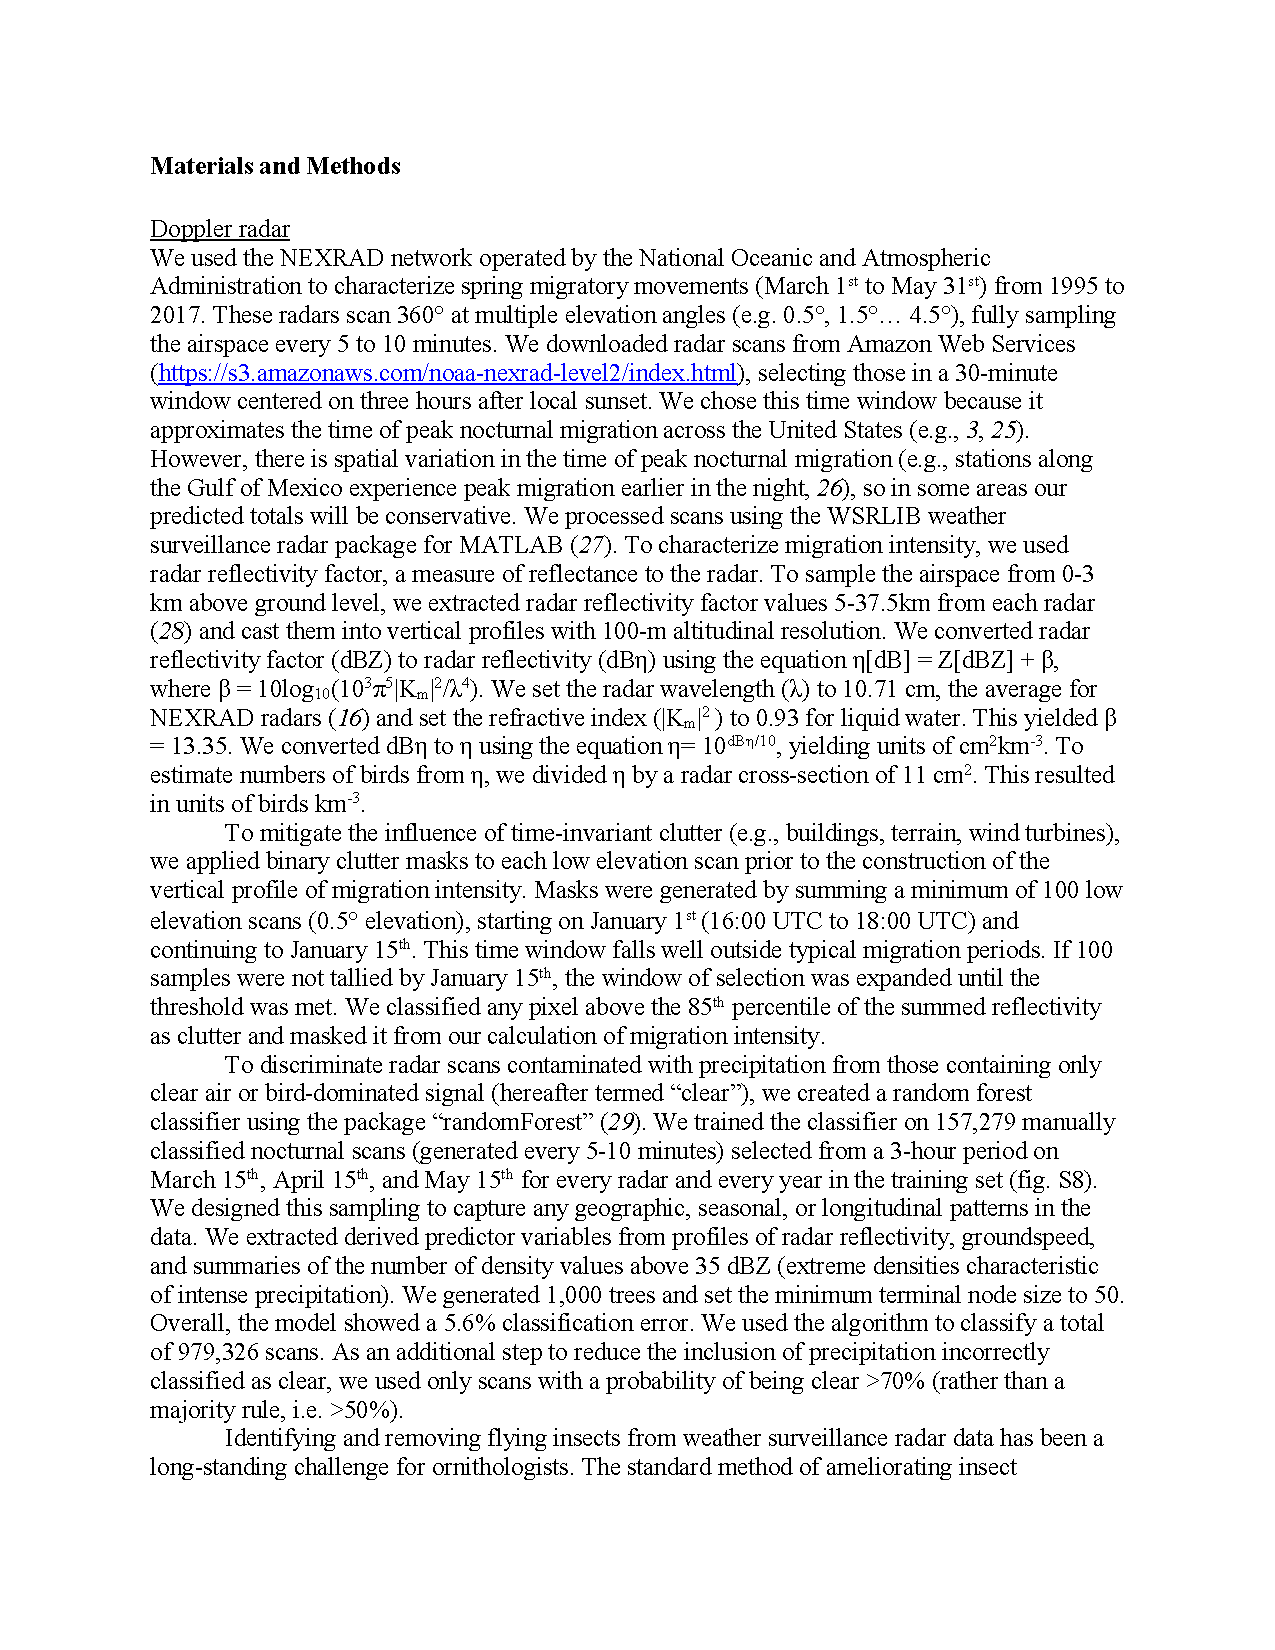
\includegraphics[width=1.1\linewidth]{/Users/Benjamin/Documents/Oxford/Thesis/oxforddown/pdf_chapters/forecast/forecast_supp_crop_Part02.pdf}} \end{center} \newpage 
 \begin{center} \makebox[\linewidth][c]{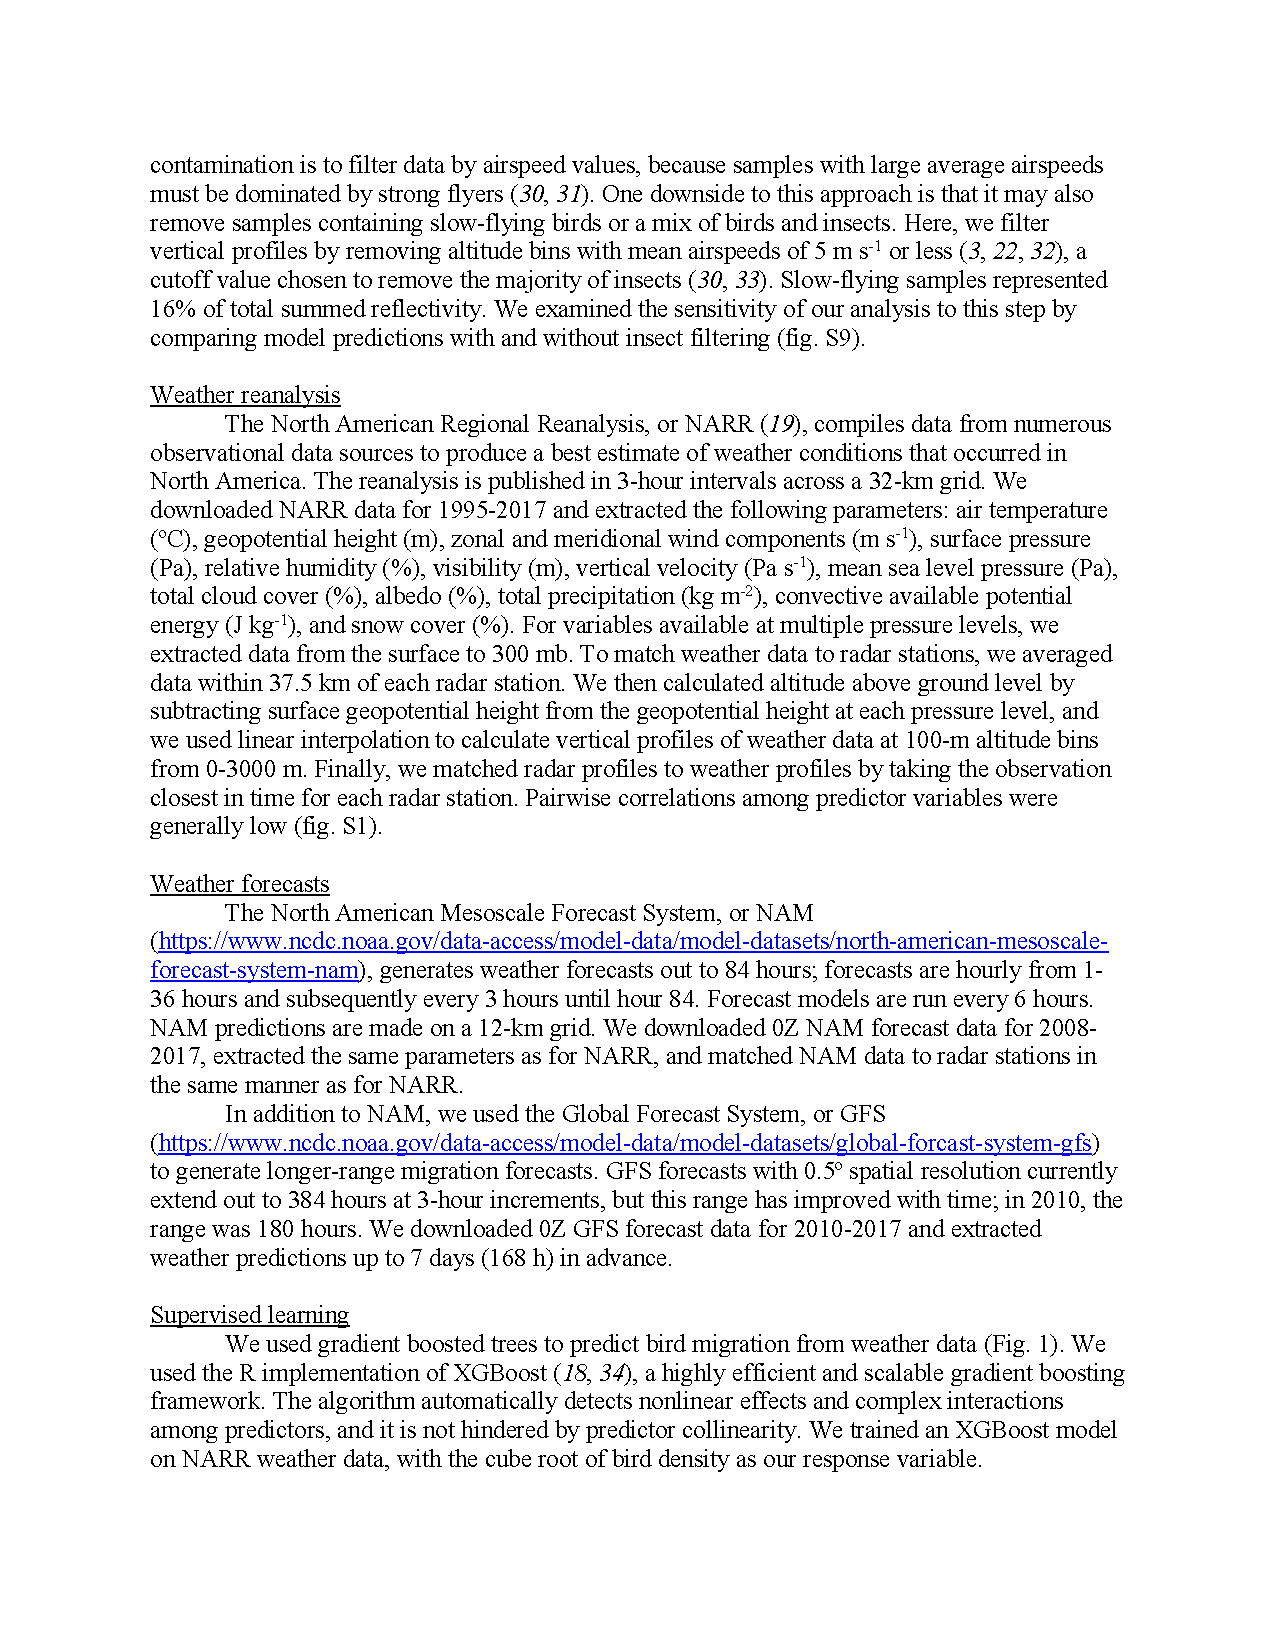
\includegraphics[width=1.1\linewidth]{/Users/Benjamin/Documents/Oxford/Thesis/oxforddown/pdf_chapters/forecast/forecast_supp_crop_Part03.pdf}} \end{center} \newpage 
 \begin{center} \makebox[\linewidth][c]{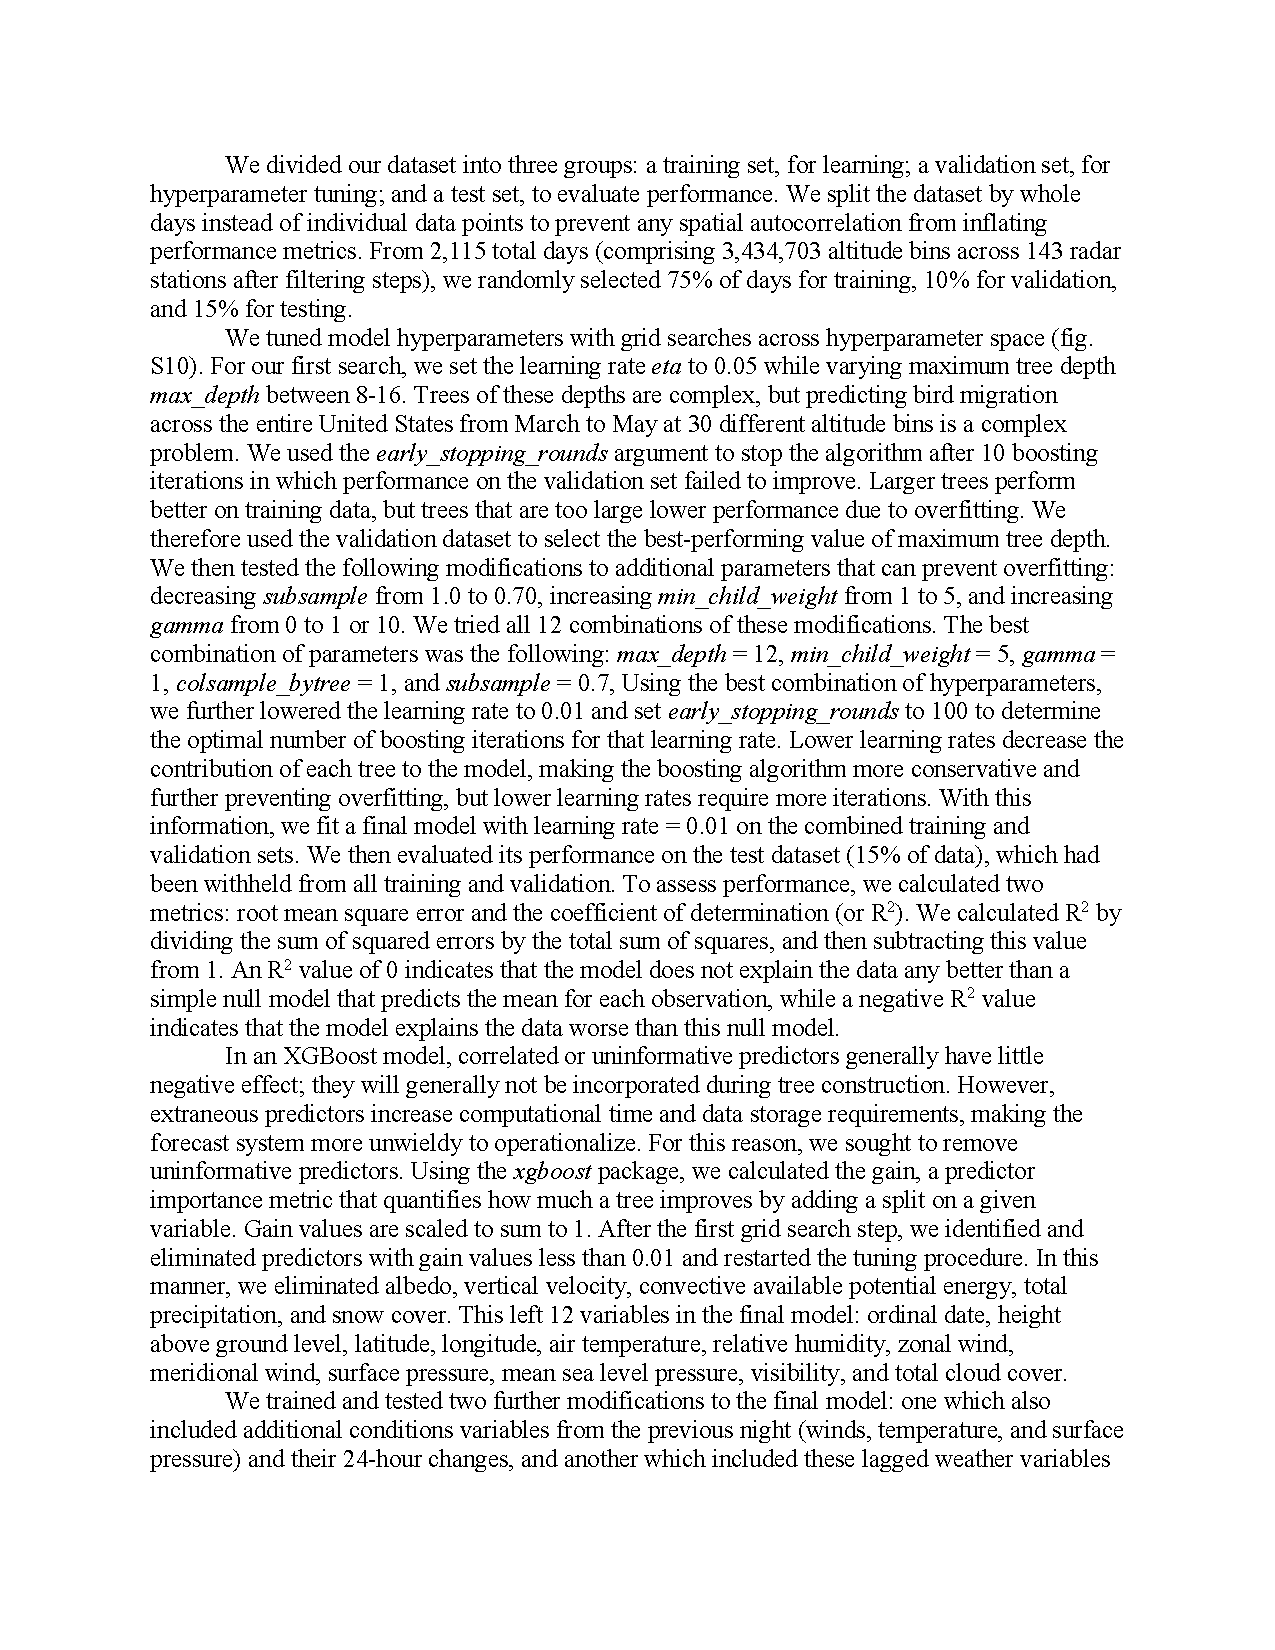
\includegraphics[width=1.1\linewidth]{/Users/Benjamin/Documents/Oxford/Thesis/oxforddown/pdf_chapters/forecast/forecast_supp_crop_Part04.pdf}} \end{center} \newpage 
 \begin{center} \makebox[\linewidth][c]{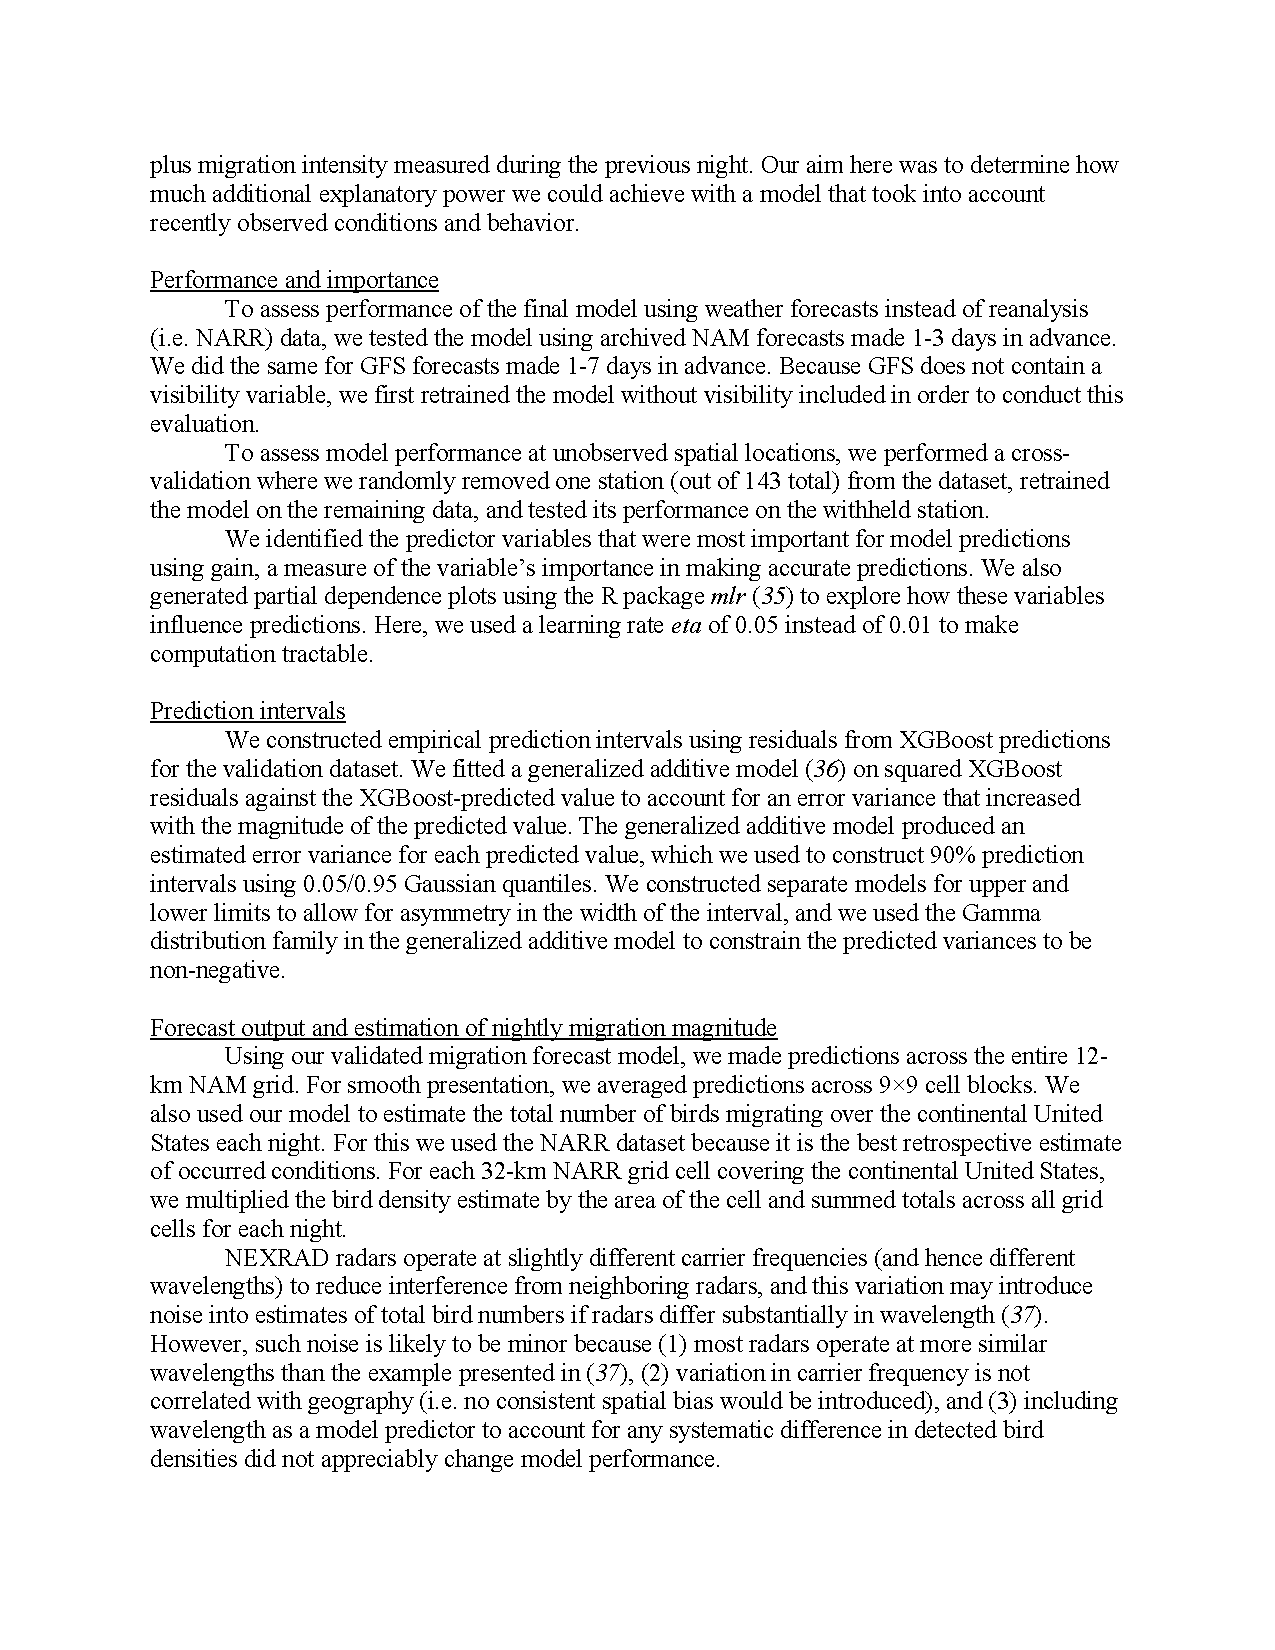
\includegraphics[width=1.1\linewidth]{/Users/Benjamin/Documents/Oxford/Thesis/oxforddown/pdf_chapters/forecast/forecast_supp_crop_Part05.pdf}} \end{center} \newpage 
 \begin{center} \makebox[\linewidth][c]{\includegraphics[width=1.1\linewidth]{/Users/Benjamin/Documents/Oxford/Thesis/oxforddown/pdf_chapters/forecast/forecast_supp_crop_Part06.pdf}} \end{center} \newpage 
 \begin{center} \makebox[\linewidth][c]{\includegraphics[width=1.1\linewidth]{/Users/Benjamin/Documents/Oxford/Thesis/oxforddown/pdf_chapters/forecast/forecast_supp_crop_Part07.pdf}} \end{center} \newpage 
 \begin{center} \makebox[\linewidth][c]{\includegraphics[width=1.1\linewidth]{/Users/Benjamin/Documents/Oxford/Thesis/oxforddown/pdf_chapters/forecast/forecast_supp_crop_Part08.pdf}} \end{center} \newpage 
 \begin{center} \makebox[\linewidth][c]{\includegraphics[width=1.1\linewidth]{/Users/Benjamin/Documents/Oxford/Thesis/oxforddown/pdf_chapters/forecast/forecast_supp_crop_Part09.pdf}} \end{center} \newpage 
 \begin{center} \makebox[\linewidth][c]{\includegraphics[width=1.1\linewidth]{/Users/Benjamin/Documents/Oxford/Thesis/oxforddown/pdf_chapters/forecast/forecast_supp_crop_Part10.pdf}} \end{center} \newpage 
 \begin{center} \makebox[\linewidth][c]{\includegraphics[width=1.1\linewidth]{/Users/Benjamin/Documents/Oxford/Thesis/oxforddown/pdf_chapters/forecast/forecast_supp_crop_Part11.pdf}} \end{center} \newpage 
 \begin{center} \makebox[\linewidth][c]{\includegraphics[width=1.1\linewidth]{/Users/Benjamin/Documents/Oxford/Thesis/oxforddown/pdf_chapters/forecast/forecast_supp_crop_Part12.pdf}} \end{center} \newpage 
 \begin{center} \makebox[\linewidth][c]{\includegraphics[width=1.1\linewidth]{/Users/Benjamin/Documents/Oxford/Thesis/oxforddown/pdf_chapters/forecast/forecast_supp_crop_Part13.pdf}} \end{center} \newpage 
 \begin{center} \makebox[\linewidth][c]{\includegraphics[width=1.1\linewidth]{/Users/Benjamin/Documents/Oxford/Thesis/oxforddown/pdf_chapters/forecast/forecast_supp_crop_Part14.pdf}} \end{center} \newpage 
 \begin{center} \makebox[\linewidth][c]{\includegraphics[width=1.1\linewidth]{/Users/Benjamin/Documents/Oxford/Thesis/oxforddown/pdf_chapters/forecast/forecast_supp_crop_Part15.pdf}} \end{center} \newpage 
 \begin{center} \makebox[\linewidth][c]{\includegraphics[width=1.1\linewidth]{/Users/Benjamin/Documents/Oxford/Thesis/oxforddown/pdf_chapters/forecast/forecast_supp_crop_Part16.pdf}} \end{center} \newpage 
 \begin{center} \makebox[\linewidth][c]{\includegraphics[width=1.1\linewidth]{/Users/Benjamin/Documents/Oxford/Thesis/oxforddown/pdf_chapters/forecast/forecast_supp_crop_Part17.pdf}} \end{center} \newpage 
 \begin{center} \makebox[\linewidth][c]{\includegraphics[width=1.1\linewidth]{/Users/Benjamin/Documents/Oxford/Thesis/oxforddown/pdf_chapters/forecast/forecast_supp_crop_Part18.pdf}} \end{center} \newpage

\part{Migration in the Anthropocene}

\begin{savequote}
\textbf{Van Doren, B.M.},* Horton, K.G.,* Dokter, A.M., Klinck, H.,
Elbin, S.B., and Farnsworth, A. (2017). High-intensity urban light
installation dramatically alters nocturnal bird migration.\\
\emph{PNAS} 114, 11175--11180.

\begin{scriptsize} * Equal contributions. \end{scriptsize}
\end{savequote}

\hypertarget{lights}{
\chapter[High-intensity artificial light alters bird migration]{High-intensity artificial light\\alters bird migration}\label{lights}}

\newpage

\begin{center} \makebox[\linewidth][c]{\includegraphics[width=1.2\linewidth]{/Users/Benjamin/Documents/Oxford/Thesis/oxforddown/pdf_chapters/lights/lights_crop_Part1.pdf}} \end{center} \newpage 
 \begin{center} \makebox[\linewidth][c]{\includegraphics[width=1.2\linewidth]{/Users/Benjamin/Documents/Oxford/Thesis/oxforddown/pdf_chapters/lights/lights_crop_Part2.pdf}} \end{center} \newpage 
 \begin{center} \makebox[\linewidth][c]{\includegraphics[width=1.2\linewidth]{/Users/Benjamin/Documents/Oxford/Thesis/oxforddown/pdf_chapters/lights/lights_crop_Part3.pdf}} \end{center} \newpage 
 \begin{center} \makebox[\linewidth][c]{\includegraphics[width=1.2\linewidth]{/Users/Benjamin/Documents/Oxford/Thesis/oxforddown/pdf_chapters/lights/lights_crop_Part4.pdf}} \end{center} \newpage 
 \begin{center} \makebox[\linewidth][c]{\includegraphics[width=1.2\linewidth]{/Users/Benjamin/Documents/Oxford/Thesis/oxforddown/pdf_chapters/lights/lights_crop_Part5.pdf}} \end{center} \newpage 
 \begin{center} \makebox[\linewidth][c]{\includegraphics[width=1.2\linewidth]{/Users/Benjamin/Documents/Oxford/Thesis/oxforddown/pdf_chapters/lights/lights_crop_Part6.pdf}} \end{center} \newpage

\begin{center} \makebox[\linewidth][c]{\includegraphics[width=1.2\linewidth]{/Users/Benjamin/Documents/Oxford/Thesis/oxforddown/pdf_chapters/lights/lights_supp_crop_Part05.pdf}} \end{center} \newpage 
 \begin{center} \makebox[\linewidth][c]{\includegraphics[width=1.2\linewidth]{/Users/Benjamin/Documents/Oxford/Thesis/oxforddown/pdf_chapters/lights/lights_supp_crop_Part06.pdf}} \end{center} \newpage 
 \begin{center} \makebox[\linewidth][c]{\includegraphics[width=1.2\linewidth]{/Users/Benjamin/Documents/Oxford/Thesis/oxforddown/pdf_chapters/lights/lights_supp_crop_Part07.pdf}} \end{center} \newpage 
 \begin{center} \makebox[\linewidth][c]{\includegraphics[width=1.2\linewidth]{/Users/Benjamin/Documents/Oxford/Thesis/oxforddown/pdf_chapters/lights/lights_supp_crop_Part08.pdf}} \end{center} \newpage 
 \begin{center} \makebox[\linewidth][c]{\includegraphics[width=1.2\linewidth]{/Users/Benjamin/Documents/Oxford/Thesis/oxforddown/pdf_chapters/lights/lights_supp_crop_Part09.pdf}} \end{center} \newpage 
 \begin{center} \makebox[\linewidth][c]{\includegraphics[width=1.2\linewidth]{/Users/Benjamin/Documents/Oxford/Thesis/oxforddown/pdf_chapters/lights/lights_supp_crop_Part10.pdf}} \end{center} \newpage 
 \begin{center} \makebox[\linewidth][c]{\includegraphics[width=1.2\linewidth]{/Users/Benjamin/Documents/Oxford/Thesis/oxforddown/pdf_chapters/lights/lights_supp_crop_Part11.pdf}} \end{center} \newpage 
 \begin{center} \makebox[\linewidth][c]{\includegraphics[width=1.2\linewidth]{/Users/Benjamin/Documents/Oxford/Thesis/oxforddown/pdf_chapters/lights/lights_supp_crop_Part12.pdf}} \end{center} \newpage 
 \begin{center} \makebox[\linewidth][c]{\includegraphics[width=1.2\linewidth]{/Users/Benjamin/Documents/Oxford/Thesis/oxforddown/pdf_chapters/lights/lights_supp_crop_Part13.pdf}} \end{center} \newpage 
 \begin{center} \makebox[\linewidth][c]{\includegraphics[width=1.2\linewidth]{/Users/Benjamin/Documents/Oxford/Thesis/oxforddown/pdf_chapters/lights/lights_supp_crop_Part14.pdf}} \end{center} \newpage 
 \begin{center} \makebox[\linewidth][c]{\includegraphics[width=1.2\linewidth]{/Users/Benjamin/Documents/Oxford/Thesis/oxforddown/pdf_chapters/lights/lights_supp_crop_Part15.pdf}} \end{center} \newpage 
 \begin{center} \makebox[\linewidth][c]{\includegraphics[width=1.2\linewidth]{/Users/Benjamin/Documents/Oxford/Thesis/oxforddown/pdf_chapters/lights/lights_supp_crop_Part16.pdf}} \end{center} \newpage 
 \begin{center} \makebox[\linewidth][c]{\includegraphics[width=1.2\linewidth]{/Users/Benjamin/Documents/Oxford/Thesis/oxforddown/pdf_chapters/lights/lights_supp_crop_Part17.pdf}} \end{center} \newpage 
 \begin{center} \makebox[\linewidth][c]{\includegraphics[width=1.2\linewidth]{/Users/Benjamin/Documents/Oxford/Thesis/oxforddown/pdf_chapters/lights/lights_supp_crop_Part18.pdf}} \end{center} \newpage 
 \begin{center} \makebox[\linewidth][c]{\includegraphics[width=1.2\linewidth]{/Users/Benjamin/Documents/Oxford/Thesis/oxforddown/pdf_chapters/lights/lights_supp_crop_Part19.pdf}} \end{center} \newpage

\begin{savequote}
\textbf{Van Doren, B.M.}, Conway, G.J., Phillips, R.J., Evans, G.C.,
Roberts, G.C.M., Liedvogel, M., and Sheldon, B.C. 
\end{savequote}

\hypertarget{blackcap-uk}{
\chapter[Human activity shapes the winter ecology of blackcaps]{Human activity shapes the\\winter ecology of blackcaps}\label{blackcap-uk}}

\hypertarget{abstract}{%
\section{Abstract}\label{abstract}}

Human behavior profoundly affects the natural world. Migratory birds are particularly susceptible to adverse effects because the global networks of ecosystems on which they rely are undergoing rapid transformation. The blackcap (\emph{Sylvia atricapilla}) is one of few migratory species thriving in this changing, human-dominated world. Its recent establishment of a high-latitude wintering population in the British Isles has been linked to climate change and supplementary garden bird feeding. We studied this wintering population to understand the landscape-scale drivers of its new distribution, interactions with supplementary food resources, and anthropogenic influences on its movement behavior and ecology. We found that blackcaps wintering in Britain were strongly associated with suburban areas and preferred warmer climates, suggesting an important role of human-modified landscapes and recent climatic shifts in facilitating the species' winter range expansion. High reliability of supplemental food may select for winter movement behavior different from the itinerancy characteristic of traditional wintering areas; in Britain, we detected relatively high site fidelity and low transience among wintering locations. Individuals tracked with geolocators generally stayed at garden sites until immediately before spring departure, suggesting that experiences in gardens may have direct carry-over effects to the breeding season. Nonetheless, blackcaps did not exclusively feed in gardens, and visits were mainly associated with periods of harsh weather. Supplemental food hence may benefit survival, but it does not define their diet. Most striking was a high degree of individual variation in movement behavior and interactions. It may be this variability, and the flexibility it imparts, that has allowed the blackcap to flourish despite global environmental change.

\hypertarget{introduction}{%
\section{Introduction}\label{introduction}}

Humans are increasingly influencing the natural world. Organisms of all kinds are affected by a range of pressures, including effects of development and agriculture on natural habitats; changing temperature and precipitation regimes wrought by climate change; hunting and exploitation; and light and noise pollution \autocite{gastonEcologicalImpactsNighttime2013,hanskiHabitatLossDynamics2011,mantyka-pringleInteractionsClimateHabitat2012,benitez-lopezImpactHuntingTropical2017,kuncAquaticNoisePollution2016,urbanAcceleratingExtinctionRisk2015}. Organisms differ in their ability to adjust to environmental change, and the extent to which ecological communities will be able to keep pace is unclear \autocite{feeleyAmazonVulnerabilityClimate2012,liangHowDisturbanceCompetition2018,poloczanskaGlobalImprintClimate2013,urbanImprovingForecastBiodiversity2016}. Migratory birds are key to ecosystem health \autocite{bauerMigratoryAnimalsCouple2014}, but they are particularly susceptible to environmental change because successful migration requires the integration of a number of disparate components, each one sensitive to ongoing changes that may be poorly correlated. Migrants must time their journeys precisely, navigate accurately through a dynamic atmosphere, locate resources safely, reliably and efficiently, and thrive in ecological contexts that differ across seasons and hemispheres. As climate change shifts optimal timing windows, wind regimes, and storm patterns, and as humans modify both the landscapes through which birds pass and the areas where they breed and winter, a migratory strategy may become increasingly untenable \autocite{wilcoveGoingGoingGone2008,rungeProtectedAreasGlobal2015}. Migrant birds are in decline in multiple regions, in part because many lack the flexibility to rapidly respond and adapt to these large scale environmental changes \autocite{beresfordPhenologyClimateChange2019,bothAvianPopulationConsequences2010,fraserIndividualVariabilityMigration2019,sandersonLongtermPopulationDeclines2006}.

Whether migratory species have the capacity to adjust to rapid change is a focal question of current research. Although plasticity in response to climate change is well documented \autocite{gienappResponsesClimateChange2007,usuiTemporalShiftsTemperature2017}, many migratory birds, especially long-distance travelers, rely on innate timing and navigational programs with limited flexibility \autocite{akessonTimingAvianLongdistance2017,gwinnerCircannualClocksAvian1996}. These programs must undergo evolution for adjustments to be realized. There is some evidence that microevolutionary change---not just plasticity---may be occurring, but it is unclear whether this can match the pace of warming \autocites[Chapter \ref{flycatchers}:][]{helmEvolutionaryResponseClimate2019}{vanbuskirkPhenotypicPlasticityAlone2012}{charmantierClimateChangeTiming2014}{merilaClimateChangeAdaptation2014}. As changes continue, species will not only need to shift timing but also undergo large-scale distributional changes to track suitable conditions. Climate-induced range shifts have been documented in birds \autocite{ambrosiniClimateChangeLongterm2011,lehikoinenNorthNorthwestClimate2016,lasortePolewardShiftsWinter2007,tingleyPushPullClimate2012}, but we lack an understanding of the ecological and behavioral processes that facilitate these shifts. This poses a challenge for predicting how species will respond in the future.

The Eurasian blackcap (\emph{Sylvia atricapilla}) is one of few migratory songbirds thriving in the face of environmental change \autocite{ebcc/birdlife/rspb/csoTrendsCommonBirds2018}. This widespread species shows a spectrum of migratory strategies from sedentary to fully migratory \autocite{crampSylviaAtricapillaBlackcap1992}, and it has experienced substantial and continuing population increases across Europe \autocite[+155\% since 1980;][]{ebcc/birdlife/rspb/csoTrendsCommonBirds2018}. In addition, the blackcap has expanded its European wintering range northward in the last half century, most notably in the British Isles, where its status has changed from a rare visitor to an established component of the winter avifauna in some regions \autocite{franssonWinteringBlackcapsSylvia1994,fouargePointCasHivernage1980,johansenVinterforekomstAfMunk2002,bearhopAssortativeMatingMechanism2005,bertholdMigratoryBehaviourPopulation1988,bertholdRapidMicroevolutionMigratory1992,leachWinteringBlackcapsBritain1981}. This transformation has been hypothesized to be linked to human activity in two ways \autocite{bertholdMigratoryBehaviourPopulation1988,plummerSupplementaryFeedingGardens2015}: first, climate change has resulted in milder winters, and second, abundant garden feeding stations now provide a reliable food source through the winter. Surprisingly, available evidence \autocites[Chapter \ref{blackcap-geo};][]{bertholdRapidMicroevolutionMigratory1992}{plummerSupplementaryFeedingGardens2015}{wernhamMigrationAtlasMovements2002} indicates that virtually all British overwinterers are \emph{not} residents that originate from British breeding populations, but rather are visitors from continental Europe that undertake highly atypical northwesterly migrations in autumn. These individuals differ from those that use traditional Mediterranean winter areas in a number of important ways: they use a novel migratory direction, winter at higher latitudes, utilize human-dominated habitats, and are closely associated with supplementary food provided by humans. Blackcaps wintering in the British Isles have adapted to many of the characteristic features of the Anthropocene, and understanding the processes linked to their success will help us understand what it takes for a migratory bird to succeed in the face of global change.

Here, we study the ecology and behavior of blackcaps wintering in the British Isles across scales. We start with a landscape analysis of the species' distribution in this newly established wintering region and use these insights to inform individual-based analyses of movement and behavior. We use two nationwide winter bird atlases conducted from 1981--1984 \autocite{blandBlackcap1986} and 2007--2011 \autocite{balmer2013bird} to examine the associations between blackcap distribution and weather, climate, land use, and fruit-producing plants over time. Previous research using a 12-year dataset from observers in British gardens showed that blackcap presence is increasingly associated with garden bird feeding and warmer climates \autocite{plummerSupplementaryFeedingGardens2015}. We build on this work by taking a landscape-scale perspective not exclusive to garden sites, examining associations with a range of climate and land cover variables, and testing for biotic interactions with potentially important food plants (holly, ivy, mistletoe, and traditional orchards).

Because a landscape-scale study contains limited information on the behavior of individual birds, we conduct a complementary analysis using ringing recoveries and a detailed dataset of individual captures and resightings. We study how individually-marked birds utilize garden habitats and food resources and how their behavior is influenced by local environmental conditions. We hypothesize that blackcaps are not wholly reliant on supplementary food throughout the winter, but that it may be a lifeline during challenging conditions. We also examine the site fidelity of individuals between winters. Studies in Mediterranean and African wintering areas report winter blackcap recapture rates of only 0--5\% in subsequent years \autocite{cuadradoAllBlackcapsSylvia1995,cuadradoYearYearRecurrence1992,kingSiteFidelityRecurrence2001,loveiMigrationWinteringBlackcap1985}; we investigate whether British overwinterers have adopted greater site fidelity to take advantage of more reliable garden feeding sites. We use ringing data to study movements within and across winters, and we combine ringing with individual tracking to examine the breeding origins of wintering blackcaps. Finally, we compare sighting records and geolocator tracks to examine the hypothesis that the high-quality food available in gardens plays an important role in migratory fueling.

\hypertarget{methods-1}{%
\section{Methods}\label{methods-1}}

\hypertarget{winter-bird-atlases}{%
\subsection{Winter Bird Atlases}\label{winter-bird-atlases}}

We used two international bird atlases to study the drivers of blackcap winter distribution in the UK. The UK and Ireland undertook combined avian winter atlases from 1981--1984 and 2007--2011. The 1981--84 atlas sampled across a 10x10 km grid, and the 2007--2011 atlas primarily used finer 2x2 km resolution. In order to make direct comparisons between atlases, we aggregated records from 2007--2011 to 10x10 km (Figure \ref{fig:site-fig}AB). We focused on Britain for this analysis because it matched the geographic extent of our land cover and climate data.

In both 1981--84 and 2007--11 atlases, observers recorded birds detected within grid cells, but the survey methodology differed. In 1981--84, surveyors visited 10x10 km grid cells and recorded the duration of their survey. In addition, they recorded casual observations without associated effort data. In 2007--11, surveyors also used a combination of standardized timed counts and opportunistic visits with unrecorded effort. In addition, the 2007--11 atlas included data from BirdTrack, a citizen science repository. For both atlases, we only retained records with associated effort data, thereby excluding casual and opportunistic records.

Due to the methodological differences between atlases, we were unable to estimate and directly compare relative abundance. Instead, we converted atlas data into a binary variable for each 10x10 km grid cell, set to one if at least one blackcap was detected during the atlas, and zero if effort was put in but no blackcaps were detected. For 1981--84, we used the recorded survey duration per 10x10 km cell visit as our measure of effort in that cell. For 2007--11, we used a similar measure: the sum of the duration of timed counts that took place with the 10x10 km cell. In this way, we assigned zeros to cells where no blackcaps were detected despite survey effort. We excluded cells with no survey effort from our analysis.

\hypertarget{climate-data}{%
\subsection{Climate data}\label{climate-data}}

We compiled environmental data from a number of sources for comparison with winter bird atlas data. First, we used the 10 m vector land map from Natural Earth {[}\url{http://naturalearthdata.com}{]} for land and water boundaries and to determine the land area of each grid cell. We downloaded historical climate data from the \emph{HadUK-Grid} dataset available from the UK Met Office {[}\url{https://www.metoffice.gov.uk/research/climate/maps-and-data/data/haduk-grid/overview}{]}.

To capture variation in climate across the British Isles, we used the 30-year monthly averages from 1981--2010 provided in the HadUK dataset. This temporal scope aligned closely with our study period. We downloaded the following variables: average of daily maximum, minimum, and mean air temperature; total precipitation; surface wind; number of days with ground frost; and number of days with snow on the ground. The data are provided at a 1x1 km resolution, which we aggregated to the necessary spatial resolution and averaged from November to March.

To capture annual variation in weather conditions across each winter, we downloaded yearly HadUK datasets summarized by month for the same variables as above. In our yearly measures, we were primarily interested in capturing annual deviations from the long term average (e.g.~a colder-than-average winter). Therefore, we modified yearly measures by subtracting the 30-year average from the yearly data. Our final weather dataset thus includes 30-year climatic data, as well as yearly deviations from those 30-year averages.

\hypertarget{plant-distributions}{%
\subsection{Plant distributions}\label{plant-distributions}}

We investigated whether the distributions of certain key plant species are associated with blackcaps' winter distribution in the British Isles. We downloaded observational data from the New Atlas of the British and Irish Flora recording scheme, courtesy of the Botanical Society of Britain \& Ireland, for three plant species:
ivy (\emph{Hedera helix}),
holly (\emph{Ilex aquifolium}), and
mistletoe (\emph{Viscum album}). We selected these species because their fruits are well-documented blackcap winter food sources \autocite{snowBirdsBerries2010,hardyWinterFoodsBlackcaps1978,leachWinteringBlackcapsBritain1981}. We downloaded observations at the 10x10 km grid level, requesting the number of 2x2 km cells for which observations had been submitted since 1970. We then summed the number of occupied 2x2 cells for each 10x10 cell as a relative measure of pseudo-abundance for that species. We elected to use this approach due to its simplicity and because the dataset provides high quality coverage across the British Isles.

We downloaded spatial data on the distribution of traditional orchards, given blackcaps' preference for apples provided in gardens \autocite{hardyWinterFoodsBlackcaps1978,leachWinteringBlackcapsBritain1981}. Data for England was provided by Natural England {[}\url{https://naturalengland-defra.opendata.arcgis.com/datasets/traditional-orchards-hap-provisional-england}{]} and data for Wales from Lle {[}\url{http://lle.gov.wales/catalogue/item/TraditionalOrchards}{]}. We could not obtain data for Scotland, however traditional orchards in Scotland represent less than 1\% of total traditional orchard area in Britain \autocite{brigUKBiodiversityAction2008}. We quantified traditional orchard coverage by summing the total area occupied by orchards in each 10x10 km cell and calculating the proportion of land area occupied by traditional orchards. We set all cells in Scotland to have a value of zero.

\hypertarget{land-cover}{%
\subsection{Land cover}\label{land-cover}}

We used land cover data from the UK Centre for Ecology \& Hydrology {[}\url{https://www.ceh.ac.uk/services/land-cover-map-2015\#data}{]}. We downloaded the 1 km raster version of the latest release, \emph{LCM2015}. This dataset classifies each 1 km square in Britain to one of a number of land cover classes. We used the 10 broad ``aggregate'' classes, with three exceptions. In place of the aggregate class ``built-up areas and gardens,'' we used the more specific ``suburban'' and ``urban'' target classes. We removed ``freshwater'' and ``saltwater'' classes because these are not directly relevant to this species. This left the following nine classes: broadleaf woodland, coniferous woodland, arable land, improved grassland, semi-natural grassland, mountain/heath/bog, coastal, urban, and suburban. We created predictor variables describing the percent land cover occupied by these land cover classes in each 10x10 km cell.

\hypertarget{refining-spatial-predictors}{%
\subsection{Refining spatial predictors}\label{refining-spatial-predictors}}

We examined predictors to remove highly correlated variables, defined as correlation coefficient \textgreater{} 0.75. For correlated predictors, we retained the predictor that was likely to be most informative or most biologically relevant for understanding relationships with blackcap distributions. We removed holly (correlated with ivy) and 30-year averages of ground frost, snow cover, and minimum temperature (all correlated with mean temperature). This left the following predictors: land cover variables of broadleaf woodland, coniferous woodland, arable land, improved grassland, semi-natural grassland, mountain/heath/bog, coastal, urban, and suburban; plant cover variables of ivy, mistletoe, and traditional orchards; 30-year climate variables of mean air temperature and rainfall; and annual deviations from the 30-year climate averages for mean air temperature, rainfall, and ground frost.

\hypertarget{occupancy-analysis}{%
\subsection{Occupancy analysis}\label{occupancy-analysis}}

We conducted an occupancy analysis using the R package \texttt{unmarked} \autocite{fiskeUnmarkedPackageFitting2011} to investigate the drivers of blackcap distribution across Britain. We summarized atlas and BirdTrack data by 10x10 grid cell for each winter, assigning a value of 1 if blackcaps were detected in that cell in the given winter and 0 if not. We fit a dynamic occupancy model \autocite{mackenzieEstimatingSiteOccupancy2003} using the \emph{colext} function. This model models four probabilities: the initial probability of occupancy at a site (\(\psi\)), yearly local colonization (\(\gamma\)) and local extinction (\(\epsilon\)) probabilities, and the probability of detecting the species when present (\(p\)).

We divided our predictor variables into groups based on \emph{a priori} hypotheses of their effects on blackcap distributions. We split our land cover variables into two groups: those related directly to human development (specifically, urban and suburban categories), and all others (``natural''). We also defined groups of the three plant cover variables (ivy, mistletoe, and traditional orchards), two climate variables (rainfall and temperature), and three annual weather deviation variables (ground frost, rainfall, and temperature).

We used the Akaike Information Criterion (AIC) to determine which predictor variable groups were most important in predicting blackcap distributions. We assembled a candidate model set with the following specifications. We modeled the initial probability of occupancy at a site with all possible combinations of the following variable groups: (1) natural land cover (seven variables), (2) developed land cover (two variables), (3) plant cover (three variables), and (4) climate (two variables). Our candidate models included either all variables in a group, or none. In addition, all initial occupancy models contained a variable describing the proportion of area in each 10x10 cell occupied by land. We modeled colonization and extinction probabilities with all possible combinations of the same four groups of predictors, with the addition of a categorical variable of atlas (1981--84 vs.~2007--11) for all models to allow for different average rates of turnover between atlases. We modeled detection probability with the following variables, which were the same for all models: atlas (to account for average differences in detection stemming from survey methodology or other factors), survey duration (no. hours surveyed within the cell), and our three annual weather variables (because detection is more likely during harsher winters as blackcaps utilize garden feeding stations) \autocite{plummerSupplementaryFeedingGardens2015}.

\hypertarget{individual-marking-and-resighting}{%
\subsection{Individual marking and resighting}\label{individual-marking-and-resighting}}

At 55 sites in Britain (Figure \ref{fig:site-fig}C), we color-ringed wintering blackcaps between November and April. We considered blackcaps to be confidently categorized as individuals wintering in Britain (as opposed to early or late migrants passing through) if they were encountered between December 1 and March 15, defining these boundaries using ringing recovery data (Figure \ref{fig:cutoff-fig}). We retained all records of these individuals. Wintering blackcaps were ringed between 19 November and 19 March and observed or recaptured between 31 October and 22 April. Capture sites were primarily suburban gardens and occasionally local parks. We gave each blackcap a unique combination of colored leg rings to enable individuals to be identifiable in the field. Most sites were active between the winters of 2016--2017 and 2019--2020, with the exception of the site run by GCMR and collaborators since 1992. The authors and volunteer observers made regular observations of individuals attending garden feeding stations throughout the winter.

Our compiled records consisted of captures (mist net or potter trap), visual resightings, and camera trap records. In total, we compiled a dataset of 8825 records of 608 color-ringed blackcaps.



\begin{figure}
\includegraphics[width=1\linewidth]{/Users/Benjamin/Documents/Oxford/Blackcaps/Blackcap_Geolocator_Analysis/blackcap_uk/figures/draft/p1_edit2-01} \caption{\textbf{Blackcap records and capture sites.} \textbf{(A)} Survey effort by 10 km grid cell in 1981--84 and 2007--2011 winter atlases, the latter also including citizen science contributions. \textbf{(B)} Grid cells in which blackcaps were detected during both periods. \textbf{(C)} Locations where wintering blackcaps were individually color-ringed for this study, with number of individuals marked. \textbf{(D)} A male blackcap in a British garden carrying a light-level geolocator. Photo by Ben Porter.}\label{fig:site-fig}
\end{figure}



\begin{figure}
\includegraphics[width=1\linewidth]{_main_files/figure-latex/cutoff-fig-1} \caption{\textbf{Defining the wintering period with ringing recovery data.} Plots show the number of blackcaps recovered either in the British Isles in summer (1 June to 1 August, suggesting they are actually British breeders) or encountered outside of the British Isles in winter (1 December to 15 March, suggesting they are not British winterers). We defined a British winterer as an individual encountered in the British Isles between 1 December and 15 March to minimize the chance of erroneously including non-winterers in our dataset.}\label{fig:cutoff-fig}
\end{figure}

\hypertarget{daily-weather}{%
\subsection{Daily weather}\label{daily-weather}}

We obtained local weather station data from the Met Office Integrated Data Archive System (MIDAS) \autocite{metofficeMetOfficeIntegrated2012} (\url{http://catalogue.ceda.ac.uk/uuid/220a65615218d5c9cc9e4785a3234bd0}). We selected MIDAS weather stations as close as possible to blackcap observation sites (between 9--30 km). We extracted (1) daily maximum air temperature (across 24 hours starting at 9 am), (2) total precipitation across the 12 hours from 6 am to 6 pm, and (3) mean wind speed and direction across the 12 hours from 6 am to 6 pm.

\hypertarget{daily-counts}{%
\subsection{Daily counts}\label{daily-counts}}

To understand the environmental factors influencing blackcap attendance at supplemental feeding stations, we counted the number of color-ringed individuals encountered daily at garden sites. For analysis, we retained data from a given site in a given winter if there were blackcap observations from at least 30 days in that winter. Thus we retained blackcap counts from 2266 days at 5 sites across 21 years. The majority of observation days came from the gardens of GCMR (72.2\%) and GCE (17.1\%).

We modeled daily counts of color-ringed blackcaps with a generalized linear mixed-effects model. We specified fixed effects of daily maximum air temperature, precipitation, wind speed, and day of year (from 1 November). Because we expected that the effect of seasonal timing might not be linear, we specified date as a smoothed predictor and fit our model using the \emph{gam} function in the R package \texttt{mgcv} \autocite{woodGeneralizedAdditiveModels2017} with Poisson distribution family. We hypothesized that blackcaps would be more likely to feed in gardens on cold and wet days with high winds, because of increased energy demands and increased difficulty finding and using natural food sources. We specified interactions of temperature \(\times\) precipitation, temperature \(\times\) wind speed, and precipitation \(\times\) wind speed because we hypothesized that the effects of precipitation and winds could be exacerbated at low temperatures and that winds could influence the effect of precipitation. We specified random effects of year and location to account for differences in the average number of blackcaps detected across years and across sites. We used the R package \texttt{standardize} to standardize predictor variables so that we could directly compare effect sizes across predictors and interpret intercepts at the average value of predictors. We simplified the model by removing non-significant interactions (P\textgreater0.05).

Our count dataset lacked zero counts, which are expected with a Poisson distribution family. To ensure that our Poisson model was not strongly affected by this violation, we also fit a model with the R package \texttt{glmmTMB} \autocite{brooksGlmmTMBBalancesSpeed2017}, which supports a truncated Poisson distribution family. This package does not support smoothed predictors, so we could could only fit a linear term of date in this model. Nonetheless, we compared it with the above \emph{gam} to verify that the choice of distribution family did not impact our conclusions.

\hypertarget{individual-visitation}{%
\subsection{Individual visitation}\label{individual-visitation}}

Our observations at gardens suggested large individual variation in blackcap behavior at garden sites. We leveraged our extensive dataset of individual observations to model the probability of individual blackcaps visiting garden feeding sites through the winter. We restricted our analysis to the well-covered sites in the previous ``daily count'' analysis. We used a binary response variable indicating whether each individual was observed on each day, restricting our analysis to the period during which the individual was observed at the site in a particular winter. We excluded individuals only encountered once in a winter. In total, we used observations of 308 individuals encountered a median of 12.5 times (range: 2--205).

We used a generalized mixed-effects model with a binomial distribution and logit link function to model the probability of an individual being detected in a garden on a particular day. We again fit the model with \emph{gam}. It included all fixed effects specified in the ``daily counts'' model, with the addition of sex, and including the smoothed term of date.
We simplified the model by removing non-significant interactions (P\textgreater0.05). We specified random effects of year, location, and individual to account for differences in the average probability of blackcap detection across years, sites, and individuals.

We calculated the proportion of variation in visitation explained by the random effects of location, year, and bird identity. We used the \texttt{rptR} package \autocite{stoffelRptRRepeatabilityEstimation2017} to quantify these variance proportions on the original variable scale and used bootstrapping (N=100) to generate 95\% confidence intervals for these estimates. We specified all fixed and random effects as described above.

\hypertarget{site-fidelity}{%
\subsection{Site fidelity}\label{site-fidelity}}

We examined the probability of a blackcap returning to the same garden in subsequent years. For each individual in our dataset, we determined whether or not it was seen in each of the three years following initial ringing. We only retained data points for sites where we had visual observation data for subsequent years. We modeled side fidelity with a binary response variable for whether the bird returned to the ringing site at least once in the three years after the winter of ringing. We included fixed effects of sex, the day of the season when the bird was first ringed, and the day the bird was last encountered during that first winter. We included random effects of ringing year and location to account for variation in the average probability of return among years and locations. We fit the generalized linear mixed-effects model with the \emph{bglmer} function in the R package \texttt{blme} \autocite{chungNondegeneratePenalizedLikelihood2013}, which extends the \emph{glmer} function in the R package \texttt{lme4} \autocite{batesFittingLinearMixedeffects2015}. This function fits mixed models in a Bayesian setting, with priors on model components that help prevent singular fits and aid convergence. We used this approach because the model did not converge when specified with \emph{glmer}.

\hypertarget{transience}{%
\subsection{Transience}\label{transience}}

Our dataset included a large number of blackcaps that were encountered only briefly. Blackcaps are known to show transience during the winter, in which a proportion of the population stays in a given area while other individuals only pass through \autocite{beldaResidentTransientDynamics2007,cuadradoYearYearRecurrence1992}. We modeled the likelihood of transience in our dataset with a binary variable of whether each individual bird was encountered for more than one day during the winter it was first captured. We also repeated the analysis after defining the presence window for transients to be one week long instead of one day. We considered observations from sites where we had at least 10 visual records of any individual blackcaps in a given winter to ensure sufficient sighting effort. We constructed a generalized linear mixed-effects model with a binomial distribution family and logit link (\emph{glmer} function in R package \texttt{lme4}). We used two fixed effects: (1) sex and (2) the day the bird was first encountered. We included random intercepts of year and location to account for variation in the average probability of transience among years and locations.

\hypertarget{movements}{%
\subsection{Movements}\label{movements}}

We examined blackcaps' movements within winters, among winters, and between winter and summer using ringing recoveries and individual tracking. Ringing data were from the British Trust for Ornithology (BTO) Ringing Scheme. We considered a bird to be present in the British Isles if the country of ringing or recovery was listed as one of the following: England, Scotland, Wales, Northern Ireland, Isle of Man, or Eire (Ireland). For resight data, we categorized blackcaps as British winterers if they were encountered between December 1 and March 15 (Figure \ref{fig:cutoff-fig}).

Given the evidence for transient individuals among wintering blackcaps visiting gardens, we used ringing data to study movements undertaken by individuals within the same winter. We filtered ringing data to individuals we were confident were wintering in the British Isles (see above), but we considered all recoveries between 1 November and 1 April to understand how these individuals moved both early and late in the season. We also used ringing data to examine movements between winters, filtering the dataset to encounters that occurred between December 1 and March 15.

We combined ringing data with tracks from light-level geolocators to identify where blackcaps wintering in the British Isles spend the summer. We filtered ringing recoveries to those of British wintering blackcaps between 15 May and 15 August. Geolocator data were from Chapter \ref{blackcap-geo}. In addition to identifying breeding locations, we compared the timing of migration as determined from geolocators to observations in gardens. Specifically, we asked how soon after disappearing from gardens in spring do blackcaps leave Britain. A short delay would suggest that gardens are an important resource for migratory fueling.

\hypertarget{results}{%
\section{Results}\label{results}}

\hypertarget{occupancy-analysis-1}{%
\subsection{Occupancy analysis}\label{occupancy-analysis-1}}

Winter bird atlases held in the British Isles from 1981--84 and 2007--11 revealed strong evidence that blackcaps' winter distribution is influenced by anthropogenic factors. All dynamic occupancy models in the 95\% confidence set (determined by AIC) included developed land cover and climate variables to model local colonization and extinction probabilities, and the best AIC model also included these variables for initial occupancy (Table \ref{tab:occ-mod-95-table}). The best model, with an AIC weight of 0.55, was favored over the next-best model by an evidence ratio of 3.2. It included climate, developed land cover and natural land cover variables for both initial occupancy and colonization/extinction dynamics. In addition, it included plant cover variables in the colonization/extinction model. See Table \ref{tab:occ-mod-best-table} and Figure \ref{fig:occ-fig} for full model results.

In the best AIC model (Table \ref{tab:occ-mod-best-table}), blackcaps showed strong positive associations with areas with warmer climates; an increase in average temperature by one standard deviation corresponded to an increase in the odds of initial occupancy by 2.2x and of colonization by 1.5x, and a strong decrease in the odds of extinction, by 0.4x. Blackcaps also showed positive associations with suburban areas, which were associated with greater odds of initial occupancy (1.8x) and colonization (1.1x) and smaller odds of extinction (0.7x). Plant cover strongly influenced colonization and extinction probabilities, with blackcaps more likely to appear in areas with more ivy, mistletoe, and orchard cover (1.5x, 1.3x and 1.2x, respectively) and less likely to disappear from those areas (0.7x, 0.8x and 0.9x, respectively).



\begin{figure}
\includegraphics[width=1\linewidth]{_main_files/figure-latex/occ-fig-1} \caption{\textbf{Dynamic occupancy model predicting blackcap occupancy in Britain.} \textbf{(A)} Shows model predictions for the best AIC model averaged across years of the 1981--84 winter bird atlas and 2007--2011 winter bird atlas. \textbf{(B)} Shows coefficient estimates for initial occupancy, colonization, and extinction components of the model, excluding coefficients for natural land cover variables. Not shown are coefficients for detection probability. All coefficients can be found in Table \ref{tab:occ-mod-best-table}.}\label{fig:occ-fig}
\end{figure}

\begingroup\fontsize{9.5}{11.5}\selectfont

\begin{longtable}{>{\raggedright\arraybackslash}p{7em}|>{\raggedright\arraybackslash}p{7em}|>{\raggedright\arraybackslash}p{7em}|r|>{\raggedleft\arraybackslash}p{3em}|>{\raggedleft\arraybackslash}p{3em}|>{\raggedleft\arraybackslash}p{3em}|>{\raggedleft\arraybackslash}p{3em}}
\caption{\label{tab:occ-mod-95-table}Occupancy models for blackcaps wintering in Britain. Shown is the 95 percent confidence set of models determined by AIC, plus the best model that does not contain developed land cover variables. The dynamic occupancy model incorporates four probabilities: initial occupancy, colonization, extinction, and detection. The first three columns show the predictors incorporated into these components. Some of these predictors refer to groupings of variables (e.g. developed land cover included both suburban and urban land cover); details in Methods. The best model evidence ratio is the ratio of the AIC weights, which can be interpreted as an evidence ratio in favor of the better model.}\\
\hline
Initial occupancy & Colonization and extinction & Detection & Par & delta AIC & AIC Wgt & cumltv Wgt & Best Model Evidence Ratio\\
\hline
land\_natural + land\_develop + climate + land\_area & atlas + land\_natural + land\_develop + plant\_cover + climate & annual\_weather + atlas + survey\_hr & 51 & 0.00 & 0.55 & 0.55 & 1.00\\
\hline
land\_natural + climate + land\_area & atlas + land\_natural + land\_develop + plant\_cover + climate & annual\_weather + atlas + survey\_hr & 49 & 2.30 & 0.17 & 0.72 & 3.15\\
\hline
land\_natural + plant\_cover + climate + land\_area & atlas + land\_natural + land\_develop + plant\_cover + climate & annual\_weather + atlas + survey\_hr & 52 & 3.79 & 0.08 & 0.80 & 6.67\\
\hline
land\_natural + land\_develop + plant\_cover + land\_area & atlas + land\_natural + land\_develop + plant\_cover + climate & annual\_weather + atlas + survey\_hr & 52 & 4.84 & 0.05 & 0.85 & 11.22\\
\hline
plant\_cover + climate + land\_area & atlas + land\_natural + land\_develop + plant\_cover + climate & annual\_weather + atlas + survey\_hr & 45 & 5.23 & 0.04 & 0.89 & 13.68\\
\hline
land\_natural + plant\_cover + land\_area & atlas + land\_natural + land\_develop + plant\_cover + climate & annual\_weather + atlas + survey\_hr & 50 & 6.86 & 0.02 & 0.91 & 30.82\\
\hline
climate + land\_area & atlas + land\_natural + land\_develop + plant\_cover + climate & annual\_weather + atlas + survey\_hr & 42 & 6.94 & 0.02 & 0.93 & 32.14\\
\hline
land\_natural + land\_develop + plant\_cover + climate + land\_area & atlas + land\_natural + land\_develop + plant\_cover + climate & annual\_weather + atlas + survey\_hr & 54 & 7.12 & 0.02 & 0.94 & 35.08\\
\hline
land\_natural + climate + land\_area & atlas + land\_natural + plant\_cover + climate & annual\_weather + atlas + survey\_hr & 45 & 17.03 & 0.00 & - & 4999.68\\
\hline
\end{longtable}
\endgroup{}

\begingroup\fontsize{9.5}{11.5}\selectfont

\begin{longtable}{l|l|l|l}
\caption{\label{tab:occ-mod-best-table}Output from occupancy model on winter bird atlases in 1981--84 and 2007--2011. This model comprises separate components modeling four probabilities: initial occupancy, colonization, extinction, and detection. Shown are odds ratios (exponentiated coefficients) and 95 percent confidence intervals. All continuous variables have been standardized to have a mean of zero and a variance of one so that coefficient estimates can be compared. The model intercept is not shown because the exponentiated intercept does not represent an odds ratio.}\\
\hline
Component & Term & Ratio & CI\\
\hline
\endfirsthead
\caption[]{\textit{(continued)}}\\
\hline
Component & Term & Ratio & CI\\
\hline
\endhead
Init. occupancy & Land cover: broadleaf woodland & 1.530 & [1.061,2.205]\\
\hline
Init. occupancy & Land cover: coniferous woodland & 2.424 & [0.946,6.211]\\
\hline
Init. occupancy & Land cover: arable land & 4.722 & [1.053,21.172]\\
\hline
Init. occupancy & Land cover: improved grassland & 3.674 & [1.039,12.998]\\
\hline
Init. occupancy & Land cover: semi-natural grassland & 1.454 & [0.408,5.185]\\
\hline
Init. occupancy & Land cover: mountain/heath/bog & 0.413 & [0.041,4.143]\\
\hline
Init. occupancy & Land cover: coastal & 1.263 & [0.951,1.678]\\
\hline
Init. occupancy & Land cover: suburban & 1.758 & [1.043,2.964]\\
\hline
Init. occupancy & Land cover: urban & 1.398 & [1.001,1.952]\\
\hline
Init. occupancy & Climate: 30-yr rainfall & 1.459 & [0.631,3.370]\\
\hline
Init. occupancy & Climate: 30-yr temp. & 2.215 & [1.317,3.726]\\
\hline
Init. occupancy & Proportion land area & 0.417 & [0.160,1.084]\\
\hline
Colonization & Atlas = 2007-11 & 0.753 & [0.589,0.962]\\
\hline
Colonization & Land cover: broadleaf woodland & 1.011 & [0.908,1.126]\\
\hline
Colonization & Land cover: coniferous woodland & 1.137 & [0.926,1.395]\\
\hline
Colonization & Land cover: arable land & 0.898 & [0.666,1.210]\\
\hline
Colonization & Land cover: improved grassland & 1.122 & [0.874,1.441]\\
\hline
Colonization & Land cover: semi-natural grassland & 1.186 & [0.911,1.543]\\
\hline
Colonization & Land cover: mountain/heath/bog & 1.198 & [0.848,1.692]\\
\hline
Colonization & Land cover: coastal & 1.056 & [0.921,1.210]\\
\hline
Colonization & Land cover: suburban & 1.107 & [0.960,1.277]\\
\hline
Colonization & Land cover: urban & 1.000 & [0.902,1.107]\\
\hline
Colonization & Plant cover: ivy & 1.467 & [1.166,1.846]\\
\hline
Colonization & Plant cover: mistletoe & 1.283 & [1.098,1.500]\\
\hline
Colonization & Orchard cover & 1.200 & [0.974,1.478]\\
\hline
Colonization & Climate: 30-yr rainfall & 0.628 & [0.469,0.841]\\
\hline
Colonization & Climate: 30-yr temp. & 1.476 & [1.151,1.893]\\
\hline
Extinction & Atlas = 2007-11 & 0.556 & [0.373,0.827]\\
\hline
Extinction & Land cover: broadleaf woodland & 0.812 & [0.678,0.972]\\
\hline
Extinction & Land cover: coniferous woodland & 2.108 & [1.066,4.168]\\
\hline
Extinction & Land cover: arable land & 0.400 & [0.229,0.699]\\
\hline
Extinction & Land cover: improved grassland & 0.521 & [0.326,0.833]\\
\hline
Extinction & Land cover: semi-natural grassland & 0.785 & [0.432,1.428]\\
\hline
Extinction & Land cover: mountain/heath/bog & 0.985 & [0.375,2.583]\\
\hline
Extinction & Land cover: coastal & 0.876 & [0.712,1.076]\\
\hline
Extinction & Land cover: suburban & 0.698 & [0.557,0.875]\\
\hline
Extinction & Land cover: urban & 0.840 & [0.727,0.972]\\
\hline
Extinction & Plant cover: ivy & 0.693 & [0.387,1.244]\\
\hline
Extinction & Plant cover: mistletoe & 0.834 & [0.694,1.002]\\
\hline
Extinction & Orchard cover & 0.877 & [0.678,1.134]\\
\hline
Extinction & Climate: 30-yr rainfall & 0.434 & [0.238,0.790]\\
\hline
Extinction & Climate: 30-yr temp. & 0.397 & [0.268,0.588]\\
\hline
Detection & Weather: ground frost & 0.932 & [0.820,1.061]\\
\hline
Detection & Weather: rainfall & 1.115 & [0.975,1.275]\\
\hline
Detection & Weather: temperature & 1.175 & [1.008,1.369]\\
\hline
Detection & Atlas = 2007-11 & 3.023 & [2.343,3.900]\\
\hline
Detection & Survey duration & 1.065 & [1.051,1.078]\\
\hline
\end{longtable}
\endgroup{}

\hypertarget{daily-counts-1}{%
\subsection{Daily counts}\label{daily-counts-1}}

Weather conditions and time of season strongly influenced garden blackcap counts (Table \ref{tab:daily-model-table}). More blackcaps were observed in colder temperatures, greater precipitation, and higher winds. In line with our predictions, the effect of temperature increased with precipitation. The effect of wind was dependent on precipitation, showing a positive relationship when there was little precipitation and a negative relationship at higher precipitation amounts; the combination of high winds and precipitation may simply discourage blackcaps from feeding altogether. Overall blackcap counts increased through the winter and began decreasing in mid-March (Figure \ref{fig:daily-indiv-figure}). The significance and directionality of these effects were generally consistent in a truncated Poisson model that included a linear instead of smooth term of date (not shown); however, in that model the interaction between wind speed and precipitation was replaced by an interaction of wind speed and temperature.

\begin{table}[!h]

\caption{\label{tab:daily-model-table}Predictors from Poisson generalized mixed-effects model of daily blackcap counts in British gardens. For fixed effects, shown are relative risk ratios (exponentiated coefficients), 95 percent confidence intervals, and P-values. Non-significant interactions have been removed. All continuous variables have been standardized to have a mean of zero and a variance of one so that coefficient estimates can be compared. The model intercept is not shown because the exponentiated intercept does not represent a relative risk ratio. For the smooth term, shown are the estimated degrees of freedom and P-value. For random terms, the standard deviation of the variance component is given.}
\centering
\fontsize{9.5}{11.5}\selectfont
\begin{tabular}{l|>{\raggedright\arraybackslash}p{9em}|l|l|l|l|l}
\hline
Type & Term & Ratio & CI & P-value & EDF & SD\\
\hline
Fixed & Max air temp. & 0.908 & [0.884,0.934] & <0.001 & - & -\\
\hline
Fixed & Precip. amount & 1.049 & [1.022,1.077] & <0.001 & - & -\\
\hline
Fixed & Mean wind speed & 1.032 & [1.004,1.061] & 0.025 & - & -\\
\hline
Fixed & Precip. amount $\times$ Mean wind speed & 0.962 & [0.935,0.990] & 0.009 & - & -\\
\hline
Fixed & Max air temp. $\times$ Precip. amount & 0.962 & [0.931,0.994] & 0.019 & - & -\\
\hline
Smooth & Days after 1 Nov & - & - & <0.001 & 8.653 & -\\
\hline
Random & Year & - & - & - & - & 0.434\\
\hline
Random & Location & - & - & - & - & 0.790\\
\hline
\end{tabular}
\end{table}

\hypertarget{individual-visitation-1}{%
\subsection{Individual visitation}\label{individual-visitation-1}}

Individual blackcaps were observed in gardens with an average daily probability of 0.16 (95\% CI {[}0.056,0.26{]}), averaged across all fixed and random predictors (Table \ref{tab:indiv-model-table}). Females attended gardens slightly less frequently than males. However, there was a great deal of individual variation in behavior. Of 154 individuals observed over total spans of at least 50 days, 30 were observed on less than 15\% of those days, while 48 were observed on at least 50\%. Unsurprisingly, individual identity explained the greatest variation in the dataset, representing 0.18 (95\% CI {[}0.14,0.23{]}) of variation in behavior. This was substantially more than location (0.05 {[}0,0.1{]}) and year (0.05 {[}0.02,0.08{]}). Blackcaps responded strongly to air temperature and precipitation, visiting more frequently in colder and wetter weather; an interaction indicated that the effect of temperature was stronger in the presence of precipitation, and the effect of wind was again dependent on precipitation (Table \ref{tab:indiv-model-table} and Figure \ref{fig:daily-indiv-figure}).



\begin{figure}
\includegraphics[width=1\linewidth]{_main_files/figure-latex/daily-indiv-figure-1} \caption{\textbf{Patterns of blackcap behavior in British gardens, showing predictions from two models.} The first model (shown in \textbf{(A)}) predicts the number of color-ringed blackcaps observed in gardens through the winter. The second model, shown in \textbf{(B--F)}, predicts the probability of a given blackcap being sighted in a garden between its first and last sightings in a winter. \textbf{(A)} Effect of date on predicted blackcap counts in British gardens, accounting for responses to weather. \textbf{(B)} Effect of date on the predicted probability of blackcap observation in British gardens, accounting for responses to weather. \textbf{(C)} Effect of precipitation (x-axis) on the probability of blackcap observation, at different air temperatures (colors). \textbf{(D)} Effect of precipitation (x-axis) on the probability of blackcap observation, at different wind speeds (colors). \textbf{(E)} Effect of wind speed (x-axis) on the probability of blackcap observation, under different precipitation conditions (colors). \textbf{(F)} Effect of temperature (x-axis) on the probability of blackcap observation, under different precipitation conditions (colors).}\label{fig:daily-indiv-figure}
\end{figure}

\begin{table}[t]

\caption{\label{tab:indiv-model-table}Predictors from binomial generalized mixed-effects model of daily blackcap presence in British gardens. For fixed effects, shown are odds ratios (exponentiated coefficients), 95 percent confidence intervals, and P-values. Non-significant interactions have been removed. All continuous variables have been standardized to have a mean of zero and a variance of one so that coefficient estimates can be compared. The model intercept is not shown because the exponentiated intercept does not represent an odds ratio. For the smooth term, shown are the estimated degrees of freedom and P-value. For random terms, the standard deviation of the variance component is given.}
\centering
\fontsize{9.5}{11.5}\selectfont
\begin{tabular}{l|>{\raggedright\arraybackslash}p{9em}|l|l|l|l|l}
\hline
Type & Term & Ratio & CI & P-value & EDF & SD\\
\hline
Fixed & Sex = Female & 0.843 & [0.666,1.066] & 0.154 & - & -\\
\hline
Fixed & Max air temp. & 0.774 & [0.745,0.803] & <0.001 & - & -\\
\hline
Fixed & Precip. amount & 1.094 & [1.056,1.134] & <0.001 & - & -\\
\hline
Fixed & Mean wind speed & 1.023 & [0.986,1.060] & 0.226 & - & -\\
\hline
Fixed & Precip. amount $\times$ Mean wind speed & 0.921 & [0.886,0.958] & <0.001 & - & -\\
\hline
Fixed & Max air temp. $\times$ Precip. amount & 0.929 & [0.887,0.972] & 0.002 & - & -\\
\hline
Smooth & Days after 1 Nov & - & - & <0.001 & 6.567 & -\\
\hline
Random & Year & - & - & - & - & 0.533\\
\hline
Random & Location & - & - & - & - & 0.754\\
\hline
Random & Bird ID & - & - & - & - & 0.904\\
\hline
\end{tabular}
\end{table}

\hypertarget{site-fidelity-1}{%
\subsection{Site fidelity}\label{site-fidelity-1}}

The overall probability of a blackcap returning to the same garden in subsequent years was 0.19 (95\% CI {[}0.086,0.37{]}). This estimate applies for birds with average first capture dates and average last encounter dates. There was no difference between males and females in return rate, and the date at which the bird was first ringed did not predict whether it would return (Table \ref{tab:fidelity-model-table}). However, birds last seen in gardens later in the winter were much more likely to return the following year. This may be due in part to early-winter movements (see below).

\begin{table}[t]

\caption{\label{tab:fidelity-model-table}Predictors from binomial generalized mixed-effects model of blackcap site fidelity to British gardens. For fixed effects, shown are odds ratios (exponentiated coefficients), 95 percent confidence intervals, and P-values. All continuous variables have been standardized to have a mean of zero and a variance of one so that coefficient estimates can be compared. The model intercept is not shown because the exponentiated intercept does not represent an odds ratio. For random effects, the standard deviation of the variance component is given.}
\centering
\fontsize{9.5}{11.5}\selectfont
\begin{tabular}{l|l|l|l|r|l}
\hline
Type & Term & Ratio & CI & P-value & SD\\
\hline
Fixed & Sex = Female & 0.687 & [0.382,1.235] & 0.210 & -\\
\hline
Fixed & Duration of presence (days) & 0.896 & [0.609,1.319] & 0.579 & -\\
\hline
Fixed & Last date encountered & 2.492 & [1.483,4.189] & 0.001 & -\\
\hline
Random & Year of ringing & - & - & - & 1.107\\
\hline
Random & Location & - & - & - & 0.547\\
\hline
\end{tabular}
\end{table}

\hypertarget{transience-1}{%
\subsection{Transience}\label{transience-1}}

The overall probability of residence (i.e.~being encountered for more than one day) for a ringed blackcap was 0.61 (95\% CI {[}0.32,0.83{]}). There was a lower probability of being encountered for more than one week: 0.48 (95\% CI {[}0.24,0.72{]}). The effects of sex and ringing date were not statistically significant (Table \ref{tab:transience-model-table}).

\begin{table}[t]

\caption{\label{tab:transience-model-table}Predictors from binomial generalized mixed-effects model of blackcap transience in British gardens. For fixed effects, shown are odds ratios (exponentiated coefficients), 95 percent confidence intervals, and P-values. All continuous variables have been standardized to have a mean of zero and a variance of one so that coefficient estimates can be compared. The model intercept is not shown because the exponentiated intercept does not represent an odds ratio. For random effects, the standard deviation of the variance component is given.}
\centering
\fontsize{9.5}{11.5}\selectfont
\begin{tabular}{l|l|l|l|r|l}
\hline
Type & Term & Ratio & CI & P-value & SD\\
\hline
Fixed & Sex = Female & 0.810 & [0.492,1.335] & 0.409 & -\\
\hline
Fixed & Date first encountered & 1.011 & [0.772,1.324] & 0.934 & -\\
\hline
Random & Year & - & - & - & 0.463\\
\hline
Random & Location & - & - & - & 1.372\\
\hline
\end{tabular}
\end{table}

\hypertarget{movements-1}{%
\subsection{Movements}\label{movements-1}}

Ringing data revealed that blackcaps wintering in the British Isles engage in within-winter movements, but movements of more than 10 km are largely restricted to November and December (Figure \ref{fig:movement-plot}AB). Movements in November averaged 139 km ± 203SD, in December averaged 34.5 km ± 152SD, and in January and February averaged only 0.706 km ± 1.16SD.

Above we show that many blackcaps return to the same garden in successive winters. Interestingly, individuals that do not show site fidelity may have moved substantial distances between winters. Ringing data showed that between-winter movements averaged 152 km ± 301SD (Figure \ref{fig:movement-plot}C). Our detailed garden sighting data showed that even individuals established in a garden in one winter may spend the following winter far from the initial site. One individual {[}N676642{]} was sighted by GCE on 63\% of days between 16 December 2017 and 4 April 2018. The following winter, it did not return to this site, but was present (and photographed) at a garden 53 km away between 7 January and 12 February 2019.



\begin{figure}
\includegraphics[width=1\linewidth]{_main_files/figure-latex/movement-plot-1} \caption{\textbf{Movements of blackcaps wintering in the British Isles from ringing recovery data and light-level geolocators.} \textbf{(A)} Ringing (red) and recovery (blue) locations of within-winter movements. \textbf{(B)} Distance of within-winter movements by ringing date. \textbf{(C)} Ringing (red) and recovery (blue) locations of between-winter movements. One recovery from Algeria and one from central France are not shown. \textbf{(D)} Wintering (open) and breeding (filled) locations of blackcaps wintering in the British Isles. Circles show capture sites and ringing recoveries, and triangles show breeding site estimates derived from geolocator data (from Chapter \ref{blackcap-geo}). For geolocation estimates, error bars indicate latitude estimates for sun angles ±1º.}\label{fig:movement-plot}
\end{figure}

\hypertarget{breeding-areas-and-migration-timing}{%
\subsection{Breeding areas and migration timing}\label{breeding-areas-and-migration-timing}}

Combining ringing recoveries and geolocator data, we observe that blackcaps wintering in the British Isles occupy a wide breeding area, spanning 2000 km across Europe (Figure \ref{fig:movement-plot}D). Estimates from geolocator data (from Chapter \ref{blackcap-geo}) suggest that the core source area for the wintering population is in western Europe (e.g.~France), whereas almost all ringing recoveries come from further east.

Geolocator data indicate that British winterers depart on spring migration between 15 March and 26 April, with a median date of 3 April (Figure \ref{fig:timing-plot}A). They return in autumn between 4 September and 22 October, with a median date of 13 October (Figure \ref{fig:timing-plot}B). We focused on observations of birds carrying geolocators at three sites with good observer coverage to determine how departure from gardens compared to migratory departure from the British Isles. After excluding individuals that left the garden shortly after being fitted with a geolocator (N=3), we found that the remaining 9 individuals departed on migration on average 4.22 ± 4.49SD days after last being seen (Figure \ref{fig:timing-plot}C). Due to short migration distances, these blackcaps typically arrived within a couple of days of departure; therefore, these birds arrived on or near the breeding grounds only 5.44 ± 5.48SD days after last being seen in their winter garden. This close correspondence between departure from the garden and departure on migration stands in contrast to the situation in autumn. In autumn, blackcaps arrived in the British Isles on average 47.7 ± 18.4SD days before being first detected by garden observers (N=12; Figure \ref{fig:timing-plot}D).



\begin{figure}
\includegraphics[width=1\linewidth]{_main_files/figure-latex/timing-plot-1} \caption{\textbf{Migration timing of British wintering blackcaps.} (\textbf{A}) and (\textbf{B}) show the distribution of departure and arrival dates; lines show uncertainty as the interquartile range of model estimates from Chapter \ref{blackcap-geo}. Spring and autumn timings are matched horizontally to the same individual. (\textbf{C}) and (\textbf{D}) compare geolocator timing estimates (blue) to the date the bird was first or last observed in the garden in which it wintered (red), in autumn and spring, respectively. Numbers give differences in days. Individuals are \emph{not} matched horizontally.}\label{fig:timing-plot}
\end{figure}

\hypertarget{discussion}{%
\section{Discussion}\label{discussion}}

\hypertarget{human-influence-on-blackcap-behavior}{%
\subsection{Human influence on blackcap behavior}\label{human-influence-on-blackcap-behavior}}

The distribution and behavior of blackcaps wintering in the British Isles is strongly shaped by human activity and mediated by environmental conditions. Our analysis shows that wintering blackcaps prefer suburban habitats, where many visit garden sites throughout the winter. Supplemental bird feeding is certainly an important driver of this pattern. Garden sites may be particularly important during periods of difficult weather, and our analysis showed increasing use of garden feeding stations in cold and wet conditions. In these conditions, foraging for berries and other fruit may be energy intensive. Access to reliable and high-energy, fatty foods, which are frequently provided in gardens, may be particularly important when birds have increased thermoregulatory requirements.

A stationary and reliable food source is unusual for a species that is primarily frugivorous during winter. Blackcaps in traditional Mediterranean wintering areas track ephemeral fruit resources or are forced to move once they are depleted \autocite{reySpatiotemporalVariationFruit1995,telleriaFruitTrackingSites2008,beldaResidentTransientDynamics2007,cuadradoYearYearRecurrence1992}. Studies in Africa and Iberia report inter-annual recapture rates of 0--5\% for wintering blackcaps \autocite{cuadradoAllBlackcapsSylvia1995,cuadradoYearYearRecurrence1992,kingSiteFidelityRecurrence2001,loveiMigrationWinteringBlackcap1985}. A capture-recapture analysis in Spain estimated that 26\% of individuals are likely to be resident at a given site during the winter, defining residency as presence for more than one week at that site \autocite{beldaResidentTransientDynamics2007}. Our estimates of return rates and residency are substantially higher: we observed an average inter-annual re-encounter probability of 0.19 (95\% CI {[}0.086,0.37{]}), and we estimated the probability of residency (\textgreater1 week) as 0.48 (95\% CI {[}0.24,0.72{]}). (However, note that we did not use capture-recapture methods to estimate this value.) We suggest that blackcaps wintering in the British Isles show lower within-winter transience and higher between-winter site fidelity due to the higher reliability of supplemental garden food sources over fruiting plants.

Wintering in the British Isles might confer a number of advantages compared to traditional southwest migratory strategies \autocite{bertholdMigratoryBehaviourPopulation1988}. Abundant supplemental food may allow blackcaps to attain better body condition and quickly amass the fat stores that will fuel their migratory flights. In turn, these factors may facilitate earlier and more successful breeding attempts. We find that blackcaps tracked with geolocators arrived at the breeding grounds on average only 5.4 days after last being seen in their gardens, suggesting that conditions at British gardens will strongly influence body condition on arrival. It is therefore plausible that the availability of reliable supplemental food puts British winterers at an advantage on the breeding grounds. The advantages of garden feeding may explain recorded differences in bill morphology between British and Iberian overwinterers \autocite{rolshausenContemporaryEvolutionReproductive2009}. Rolshausen et al.~\autocite*{rolshausenContemporaryEvolutionReproductive2009} posited that the narrower and longer bills of the British winterers in their sample may result from a more generalist diet, compared to the largely frugivorous diet of Mediterranean winterers. This difference parallels observations from Great Tits (\emph{Parus major}) in Britain, where selection for longer bills among British birds have been linked to supplementary feeding \autocite{bosseRecentNaturalSelection2017}.

\hypertarget{potential-future-changes-in-behavior}{%
\subsection{Potential future changes in behavior}\label{potential-future-changes-in-behavior}}

There is clear evidence that human activity has shaped the behavior of blackcaps wintering in the British Isles, both directly and indirectly. We found that blackcaps were more likely to occur in warmer parts of Britain, but that blackcaps were most likely to use garden sites in periods of cold and wet weather. In the coming decades, Britain is expected to continue to move towards a warmer climate \autocite{loweUKCP18ScienceOverview2018}. This is likely to improve the suitability of the region for blackcaps, but it is also likely to affect their associations with gardens. In the future, milder weather may decrease blackcaps' use of gardens, even while the wintering population increases overall.

\hypertarget{how-reliant-are-blackcaps-on-supplemental-food}{%
\subsection{How reliant are blackcaps on supplemental food?}\label{how-reliant-are-blackcaps-on-supplemental-food}}

Although supplemental bird food is likely important when winter conditions become difficult, our analysis indicates that blackcaps are far from reliant on garden feeders. In reality, we estimated that the average blackcap visits gardens with a probability of 0.16 (95\% CI {[}0.056,0.26{]}), suggesting that natural food may be sufficient much of the time. This estimate does not include transient individuals that do not frequent gardens, which represent approximately half of all blackcaps captured. Of course, it is possible that transient individuals simply move to other gardens; future radio-tracking would be a useful approach to better understand how wintering blackcaps interact with natural and artificial food sources through the winter. However, this is also consistent with the possibility that garden feeding stations may play a less pronounced role in the survival of most blackcaps wintering in the British Isles. Indeed, we found that even the most site faithful blackcaps do not appear in gardens until well after they arrive in the autumn---sometimes more than two months after arrival. The most plausible explanation is that blackcaps do not need to use garden feeding stations until natural food sources dwindle in late autumn and early winter. Consistent with this explanation, our analysis found positive associations between blackcap distributions and the distributions of ivy, mistletoe, and traditional orchards. Ivy, which ripens in late winter, may be a particularly important food source for blackcaps once other natural food has been depleted \autocite{snowBirdsBerries2010}.

\hypertarget{individual-variation-and-flexibility}{%
\subsection{Individual variation and flexibility}\label{individual-variation-and-flexibility}}

Large individual variation was a defining feature of our dataset. In our model of individual behavior in gardens, individual identity explained the greatest proportion of variation. Blackcaps existed on a continuum from frequent visitors to single-visit transients. Our results show that blackcaps exhibit a great deal of variation and flexibility in their strategies, which may be key to their success as environments rapidly change.

\hypertarget{breeding-origins-of-british-winterers-and-evidence-for-residency}{%
\subsection{Breeding origins of British winterers and evidence for residency}\label{breeding-origins-of-british-winterers-and-evidence-for-residency}}

We combined ringing recoveries and individual tracking data to show that blackcaps wintering in Britain originate from a 2000 km-wide swath of Europe (see Chapter \ref{blackcap-geo}). Ringing recoveries alone supported central European origins of the wintering population, but tracking data show that the breeding range extends well into southwest Europe, even to the Iberian Peninsula, and farther east than suggested from ringing recoveries. There were 9 recoveries of individuals encountered in the British Isles during both summer and winter, suggesting limited year-round residency. However, biases in ringing recoveries make local recaptures far more likely than external recaptures, and our tracking results indicate that at least the vast majority of wintering individuals come from outside the British Isles. None of the 25 geolocator tracks showed clear evidence for year-round residency in Britain, although one individual that wintered at Chilbolton, Hampshire, UK, spent the summer in extreme northern France or possibly the southern coast of England.

\hypertarget{conclusion-1}{%
\subsection{Conclusion}\label{conclusion-1}}

Most migratory birds facing the pressures of environmental change are in decline, but the blackcap is one of few exceptions: this species is thriving in a changing world. The recently-established wintering population of blackcaps in the British Isles provides an opportunity to understand how this species has managed to keep pace. Our results support the hypotheses that climate change combined with supplemental bird feeding has facilitated the rapid establishment of this population \autocite{plummerSupplementaryFeedingGardens2015}. Moreover, our individual-level data reveal the tremendous individual flexibility that blackcaps exhibit in their movement patterns and responses to conditions. Among migratory species, those with large variation and flexibility in movement and foraging behaviors will likely be best equipped to respond to the coming decades of environmental change.

\hypertarget{author-contributions-1}{%
\subsection{Author contributions}\label{author-contributions-1}}

BMVD conceived of the study and organized data collection with GJC, ML, and BCS, who oversaw the project. BMVD, GJC, RJP, GCE, and GCMR collected data for the study. BMVD analyzed the data and wrote the paper with input from all authors.

\hypertarget{acknowledgements-1}{%
\subsection{Acknowledgements}\label{acknowledgements-1}}

We thank Sally Amos, Jon Avon, Jake Bailey, Penny Barret, Stuart Bearhop, Rob and Liz Boon, Stuart Brown, Malcolm Burgess, Emily Cuff, Kate Dalziel, Kira Delmore, Davide Dominoni, Ian Duncan, Rachel Durham, Phil Evans, Sheila Evans, Kate Fox, Roger Francis, Lyn Gammage, Gill Garrett, Sheila Gowers and Paul Ensom, Mark Grantham, Jodie Mae Henderson, John and Jane Holmes, Emma Inzani, Brian Isles, Michael and Helen Johnson, Ben Porter, Mel Mason, Irene McGregor, Keith McMahon, Nicole Milligan, Ruedi Nager, Dee and Jonnie Reeves, Fiona Roberts, Dr ET Roberts, Gary Samways, Ash Sendell-Price, Ana Shapiro, Anna Smith, Dave Stoddard, Esmé Tackley, John Webber, Kester Wilson, Penny Witcombe, and other contributors, ringers, and homeowners.

The BTO Ringing Scheme is funded by a partnership of the British Trust for Ornithology, the Joint Nature Conservation Committee (on behalf of: Natural England, Natural Resources Wales and Scottish Natural Heritage and the Department of the Environment Northern Ireland), The National Parks and Wildlife Service (Ireland) and the ringers themselves.

This work was supported through funding from the Max Planck Society (MPRG grant to ML), the Marshall Aid Commemoration Commission (to BMVD), the American Ornithological Society (Mewaldt-King Research Award, to BMVD), the Society for the Study of Evolution (Rosemary Grant Award, to BMVD), the Frank M. Chapman Memorial Fund (to BMVD), the British Trust for Ornithology (to BMVD).

\printbibliography[segment= herefsection,heading=subbibliography]

\hypertarget{general-discussion}{%
\chapter*{General Discussion}\label{general-discussion}}
\addcontentsline{toc}{chapter}{General Discussion}

\markboth{General Discussion}{General Discussion}

\hypertarget{the-power-of-perspectives-across-scales}{%
\section*{The power of perspectives across scales}\label{the-power-of-perspectives-across-scales}}
\addcontentsline{toc}{section}{The power of perspectives across scales}

Understanding natural phenomena as complex as bird migration requires a multilevel approach, as individual-level programs and reaction norms interact with population processes and broad biotic and abiotic factors. In this thesis, I have explored several perspectives on change and flexibility in avian migration, focusing on the contributions of the innate migratory program, birds' responses to environmental cues and conditions, and the influence of human activity on migratory behavior. In \textbf{Chapter \ref{stonechats}}, I demonstrated that stonechats (genus \emph{Saxicola}) possess inherited migratory programs that vary predictably among taxa according to their migratory behavior. However, these programs are not the sole determinant of migratory phenotype, especially among partial migrants, implying that environmental factors can readily interact with the inherited program. In \textbf{Chapter \ref{flycatchers}}, I combined field and laboratory studies to present evidence of changes in the innate migratory program of a long-distance migrant, the pied flycatcher (\emph{Ficedula hypoleuca}), showing that ongoing responses of migratory birds to climate change can involve not only phenotypic plasticity, but microevolutionary change as well. In \textbf{Chapter \ref{blackcap-geo}}, I examined variation in the migratory behavior of the Eurasian blackcap (\emph{Sylvia atricapilla}) across its European range, illustrating two different ways that natural selection can act on songbird migration: (1) to maintain opposing migratory strategies over short distances, in the case of a migratory divide, and (2) to enable the spread of a novel strategy across a wide range, in the case of individuals wintering in the British Isles. In \textbf{Chapter \ref{forecast}}, I showed that migratory flexibility is important not only on evolutionary timescales, but also to enable short-term responses to variable environmental conditions during active migratory flights. These responses are predictable enough to reliably forecast avian movements across continental extents. In \textbf{Chapter \ref{lights}}, I examined how artificial light at night can drastically affect migratory journeys, an important example of anthropogenic impacts on bird migration. Finally, in \textbf{Chapter \ref{blackcap-uk}}, I returned to the blackcap to show how human activity can impact not only migrants' in-flight behaviors, but also shape their broader ecology. Overall, this body of work shows that migratory birds' flexibility stems from a range of sources, innate and external, and that the presence of variation in migratory phenotype may be key to enabling responses to environmental change.

\hypertarget{the-interplay-of-variation-and-flexibility}{%
\section*{The interplay of variation and flexibility}\label{the-interplay-of-variation-and-flexibility}}
\addcontentsline{toc}{section}{The interplay of variation and flexibility}

Variation is the engine of evolutionary change, providing populations with the raw material on which natural selection can act. Taxa with greater natural variation will be the most flexible---and best able to adapt to changing conditions.
Among migratory birds, variation and flexibility are linked: long-distance migrants with rigid timing programs show the most consistency in phenotype \autocite{gwinnerCircadianCircannualProgrammes1996,gwinnerCircadianCircannualProgrammes1996}. Shorter distance migrants show greater variation in behavior and less rigidly programmed migrations \autocite{bertholdCircannualePeriodikBei1972a,gwinnerCircannualRhythmsTropical1991}. These insights lead to the expectation that short-distance migrants will more quickly respond to climate change, a hypothesis supported by current evidence \autocite{butlerDisproportionateEffectGlobal2003,usuiTemporalShiftsTemperature2017}.

In this thesis, the contrast between short- and long-distance migrants is evident in \textbf{Chapter \ref{stonechats}}, where stonechat taxa with longer migrations showed less variation in behavior. Siberian stonechats nearly always showed migratory restlessness, whereas individuals from Irish and Kenyan populations frequently did not. Siberian stonechats are obligate long-distance migrants, Irish stonechats are partial migrants, and Kenyan stonechats are residents.

In \textbf{Chapter \ref{flycatchers}}, I observed a stark contrast between the phenotypic variation observed in the 2002 cohort of pied flycatchers and the older 1981 cohort, despite both groups having been raised under identical conditions. Although the experimental sample sizes were small, individual variation in winter and spring timing traits was greater in the 2002 cohort among both males and females. This pattern could suggest that climate change---itself variable and volatile---may be selecting for increased variation in phenotypes.

Blackcaps show broad variation in migratory traits at both individual and population levels. Populations of blackcaps range from entirely sedentary to fully migratory \autocite{crampSylviaAtricapillaBlackcap1992}, and the results from \textbf{Chapters \ref{blackcap-geo} and \ref{blackcap-uk}} highlight the variability in blackcaps' individual strategies along many axes, from migratory direction to responses to winter weather. Blackcaps breeding near the central European migratory divide showed a large spread in migratory direction as well as in timing. In British gardens, blackcaps also showed large individual variation in behavior, with some individuals reliably using garden feeding stations in a range of weather conditions and others doing so primarily during harsher weather. Blackcaps have substantial diet flexibility, which may contribute to their ability to use gardens \autocite{hardyWinterFoodsBlackcaps1978,reyDietPlasticityBlackcap1999}.

\hypertarget{taking-insights-from-the-lab-to-the-fieldand-back}{%
\section*{Taking insights from the lab to the field---and back}\label{taking-insights-from-the-lab-to-the-fieldand-back}}
\addcontentsline{toc}{section}{Taking insights from the lab to the field---and back}

Laboratory studies of migratory behavior have led to foundational insights into bird migration, including how migratory birds use the sun, stars, magnetic field, and polarized light to orient \autocite{emlenMigratoryOrientationIndigo1967,wiltschkoEvidenceInnateMagnetic1974,alerstamRoleGeomagneticField1983,akessonHowMigrantsGet2007}. Laboratory studies have also shown that songbirds' migratory behavior is innate and inherited \autocite{bertholdGeneticControlMigratory1991,helbigInheritanceMigratoryDirection1991} and even how birds respond to wind drift \autocite{ableOrientationPasserineNocturnal1977,mooreEvidenceRedeterminationMigratory1990}. At the same time, laboratory studies of migration can be limiting simply because they examine the behavior of caged birds, not free-flying individuals. Exactly how closely lab-derived assays correlate with wild phenotypes is still an open question, but recent research has shown that the migratory restlessness behavior of birds held in captivity may not always be directly comparable to migration in the wild. For example, resident populations may show migratory restlessness \autocite{helmMigratoryRestlessnessEquatorial2006}, and migrants that show restlessness every night in captivity may only undertake infrequent flights in the wild \autocite{zunigaAbruptSwitchMigratory2016,backmanActivityMigratoryFlights2017}.

This thesis affirms the value of laboratory experiments for studying migration while also illustrating why scientists should be cautious in the extent of inference drawn from lab-derived proxies of wild behavior. In \textbf{Chapter \ref{flycatchers}}, I showed that the spring timing advances of captive-raised pied flycatchers taken from the wild were of a similar magnitude to those observed in a nearby wild population. In this case, the wild and laboratory-derived data were highly complementary: by excluding plasticity as a source of timing differences, the captive study provided key insight into change in the wild population, while at the same time affirming the relevance of laboratory data for understanding wild processes. Similarly, blackcap migration has been extensively studied in a laboratory setting, and \textbf{Chapter \ref{blackcap-geo}} provides an opportunity to compare previous lab-derived insights to new migration tracks of wild birds. Captive experiments that interbred blackcaps from populations with southwest and southeast migratory directions found that their offspring showed a spread of intermediate migratory directions \autocite{helbigInheritanceMigratoryDirection1991}. The distribution of directions of wild birds tracked from the contact zone (\textbf{Chapter \ref{blackcap-geo}}) was highly similar to the distribution of directions from the experiment. However, it is important to note that these tracks were from adult blackcaps originating in the migratory divide, while Helbig measured the offspring of parental populations captured away from the contact zone. In another instance, orientation experiments with British winterers found a broadly west-northwesterly autumn orientation, in contrast to the southwesterly orientation of German blackcaps \autocite{bertholdRapidMicroevolutionMigratory1992,helbigInheritanceNovelMigratory1994}. Geolocator results showed that British winterers indeed migrate west and northwest to Britain from continental breeding areas (\textbf{Chapter \ref{blackcap-geo}}). Finally, a captive timing experiment found that blackcaps exposed to British photoperiods initiated migration on average five days earlier than those exposed to Mediterranean photoperiods, estimating that birds wintering in these two areas would arrive on the breeding grounds 16 days apart due to the shorter migration durations of British winterers \autocite{terrillEcophysiologicalAspectsRapid1990}. Results from wild-tracked blackcaps were broadly consistent with this result, yielding estimates of a six-day difference in departure and ten-day difference in arrival. Taken together, these results generally affirm the utility of laboratory experiments in the study of avian migratory behavior.

Despite clear consistencies between laboratory results and the behavior of wild-tracked migrants, this thesis also highlights the caution needed when drawing inferences from laboratory proxies of migration. In \textbf{Chapter \ref{stonechats}}, I showed that the migratory phenotypes of wild populations do not necessarily align with activity measures derived from migratory restlessness data. In that chapter, Irish stonechats, which are partial migrants \autocite[migratory individuals from Britain travel a median distance of 1139 km,][]{helmMovementsEuropeanStonechats2006}, showed intensities of spring migratory restlessness that were indistinguishable from those of Siberian stonechats, which are obligate long-distance migrants and travel upwards of 2600 km \autocite{raessContinentalEffortsMigration2008}. In addition, I detected migratory restlessness in resident Kenyan stonechats and striking changes in restlessness with age, which might be related to plasticity or poorly understood learning processes. I also found that individuals with higher nocturnal migratory restlessness tended to be more active birds overall (measured from diurnal data), which necessitates further work on how restlessness relates to other traits and caution on its exclusive interpretation as a measure of migratory tendency \autocite[e.g.~][]{bertholdEvolutionaryAspectsMigratory1988}. In blackcaps, although tracking results in \textbf{Chapter \ref{blackcap-geo}} were consistent with many insights derived from experiments in captivity (see previous paragraph), these experiments provided an incomplete picture. Orientation studies could not have determined that many blackcaps migrating south from the migratory divide would winter north of the Sahara. The experiments had concluded that a southerly migration direction would likely result in low survival \autocite{helbigInheritanceMigratoryDirection1991}, when in reality this direction is used by a large fraction of birds in the divide (\textbf{Chapter \ref{blackcap-geo}}). As a last example, Terrill and Berthold \autocite*{terrillEcophysiologicalAspectsRapid1990} used an average migration rate of 45 km per day to estimate that British winterers would take 24 days to travel from Britain to Germany on spring migration. However, data from \textbf{Chapter \ref{blackcap-geo}} indicated that the spring migrations of British winterers were often only a few days long. Overall, care is necessary when interpreting results from laboratory proxies of migratory behavior.

\hypertarget{impacts-of-human-activities-on-bird-migration}{%
\section*{Impacts of human activities on bird migration}\label{impacts-of-human-activities-on-bird-migration}}
\addcontentsline{toc}{section}{Impacts of human activities on bird migration}

This thesis examines two examples of anthropogenic impacts on bird migration systems. The first is the behavioral alterations caused by the proliferation of artificial light at night. It is not known why migratory birds are attracted or disorientated by light pollution, but its negative influence on birds has been known for some time \autocite{allenDestructionBirdsLighthouses1880}. Impacts of light pollution on birds can be severe and acute, as in cases of mass attraction and potentially mass mortality \autocite[e.g.~\textbf{Chapter \ref{lights}};][]{richEcologicalConsequencesArtificial2013}. However, this is not the only way light pollution can impact avian migrants. Recent research suggests that light at night may influence the behavior of migrating birds across a landscape scale, drawing them towards urbanized areas where suitable terrestrial habitats can be scarce \autocite{mclarenArtificialLightNight2018}. Fortunately, action to reduce light pollution can have immediate positive impacts and allow migrants to continue their flights unhindered (\textbf{Chapter \ref{lights}}).

Human activity has transformed much of the world and profoundly influenced the course of evolution of wild organisms \autocite{palumbiHumansWorldGreatest2001,boivinEcologicalConsequencesHuman2016,sullivanHumanBehaviourLongterm2017,johnsonEvolutionLifeUrban2017}. Urbanization in particular has driven major phenotypic changes \autocite{albertiGlobalUrbanSignatures2017} as organisms adapt to a human-dominated environment. As these changes reflect, one consequence of human activity is the creation of new and modified opportunities that wildlife can exploit. An obvious example of this phenomenon is the proliferation of supplemental feeding, which can have a range of impacts on the populations and behavior of wildlife \autocite{galbraithSupplementaryFeedingRestructures2015,coxHumanNatureInteractions2018,plummerCompositionBritishBird2019}. This is especially true for birds, which are frequent beneficiaries of food provisioning. At least 45\% percent of households feed birds in a number of countries, with higher provisioning rates in the United Kingdom \autocite{galbraithRisksDriversWild2014,daviesHouseholdFactorsInfluencing2012,orrosWildBirdFeeding2015}. In the UK, this behavior is an important determinant of wintering blackcap presence and a driver of their behavior \autocites[\textbf{Chapter \ref{blackcap-uk}};][]{plummerSupplementaryFeedingGardens2015}{plummerCompositionBritishBird2019}. Garden bird feeding has likely facilitated the growth of the winter blackcap population by increasing winter survival, especially when harsh conditions increase energy demands \autocite[\textbf{Chapter \ref{blackcap-uk}};][]{plummerSupplementaryFeedingGardens2015}. This example demonstrates how a bird species with sufficient flexibility in migratory behavior can take advantage of novel resources. Blackcaps are not the only species adjusting migration in response to human-mediated changes in resource availability; species as diverse as white storks (\emph{Ciconia ciconia}) and hummingbirds (Trochilidae) have adopted modified, shorter migrations \autocite{satterfieldResponsesMigratorySpecies2018}. These highly flexible species are notable because of the speed of their response, and these examples may foreshadow similar ecological shifts in the future.

\hypertarget{future-directions-and-applications}{%
\section*{Future directions and applications}\label{future-directions-and-applications}}
\addcontentsline{toc}{section}{Future directions and applications}

Natural systems are complex, reflecting the interplay among individual traits and behavior, external cues and stimuli, evolutionary processes, and other contributing factors. In this thesis, I have surveyed the drivers of bird migration across scales, seeking insights from individuals, species, and systems.

\hypertarget{dynamic-approaches-to-conservation}{%
\subsection*{Dynamic approaches to conservation}\label{dynamic-approaches-to-conservation}}
\addcontentsline{toc}{subsection}{Dynamic approaches to conservation}

This work has direct implications for conservation initiatives striving to mitigate the impacts of human society on migrating birds. \textbf{Chapter \ref{lights}} highlights the effects that artificial light can have on migrating birds, but it also shows that timely removal of light pollution can eliminate these acute impacts. Mitigation should focus on urban areas, which generate a disproportionate amount of light pollution---especially those along key migratory corridors (\textbf{Appendix \ref{app-city-lights}}). Through migration forecasts (\textbf{Chapter \ref{forecast}}), alerts could be established that warn of upcoming large migration events in time for people to turn off non-essential lighting.

\hypertarget{the-genetic-basis-of-migration}{%
\subsection*{The genetic basis of migration}\label{the-genetic-basis-of-migration}}
\addcontentsline{toc}{subsection}{The genetic basis of migration}

For decades, we have known that key aspects of songbird migration are innately programmed and have a genetic basis \autocites[e.g.~][]{bertholdGeneticBasisMigratory1981}{bertholdHeritabilityMigratoryActivity1994}{gwinnerCircannualClocksAvian1996}{helbigGeneticBasisMode1996}{pulidoFrequencyMigrantsMigratory1996}. Yet even today, we lack a meaningful understanding of the genetic architecture underlying migratory behavior. A large part of current knowledge stems from candidate genes associated with migration \autocites[e.g.~][]{muellerIdentificationGeneAssociated2011}{sainoPolymorphismClockGene2015}{johnstonSeasonalGeneExpression2016}{lugoramosCandidateGenesMigration2017}. However, detected effects of candidate genes are generally limited and taxon- or sex-specific \autocite{muellerIdentificationGeneAssociated2011,sainoPolymorphismClockGene2015,mettlerInteractionsCandidateGene2015,bazziCandidateGenesHave2017,bazziAdcyap1PolymorphismCovaries2016,parody-merinoNoEvidenceAssociation2019,ralstonLengthPolymorphismsTwo2019}, with little evidence for general patterns \autocites{lugoramosCandidateGenesMigration2017}[but see e.g.~][]{bazziClockGenePolymorphism2016}. Recent genomic work affirms a genetic basis of avian migratory behavior \autocite{delmoreGeneticsSeasonalMigration2016,toewsSelectionVPS13ALinked2019a}, but we still lack any mechanistic or unified understanding of the processes involved. Epigenetic modifications could be important \autocite{sainoMigrationPhenologyBreeding2017}. Fortunately, future work with blackcaps is promising: blackcap migration clearly has a genetic basis \autocite{bertholdRapidMicroevolutionMigratory1992,helbigInheritanceNovelMigratory1994,helbigGeneticBasisMode1996} and the species shows minimal genetic structure across its migratory populations \autocites{delmoreEvolutionaryHistoryGenomics2020}[but also see][]{rolshausenContemporaryEvolutionReproductive2009}. This scenario is encouraging for identifying genetic variants that influence migratory phenotypes. Furthermore, in \textbf{Chapter \ref{blackcap-geo}}, I illustrate that the species shows widely varying migratory strategies, as well as a narrow cline in migratory direction across the central European migratory divide. The narrow cline suggests strong selection on migratory direction (or a related trait), which may be detectable via whole genome sequencing and analysis.

\hypertarget{big-data-ecology}{%
\subsection*{``Big Data'' Ecology}\label{big-data-ecology}}
\addcontentsline{toc}{subsection}{``Big Data'' Ecology}

Ecology has entered an era of ``big data,'' and \textbf{Chapter \ref{forecast}} provides one example of the many possible uses of large datasets in understanding the natural world. Integrating multiple datasets and modeling natural processes will lead to an even greater understanding of the intricacies of complex natural systems. For scientists studying migratory birds, large Doppler radar networks are but one source of big data. Citizen science initiatives now collect millions of observations from volunteer observers, and these data repositories are invaluable resources for understanding species behavior, distributions, and responses to change \autocite[e.g.~][]{sullivanEBirdEnterpriseIntegrated2014}. Already, combining radar data and citizen science observations has led to new insights into bird migration (\textbf{Appendix \ref{app-gulf}}). As repositories of many types of data grow, it will become feasible to combine radar and citizen science data with individual tracks, acoustic monitoring, landscape genomics, and technologies that have yet to be developed. It is an exciting time to study avian migration across scales.

\printbibliography[segment=\therefsection,heading=subbibliography]

\startappendices

\hypertarget{app-stonechats-supp}{%
\chapter{Supplementary material for chapter \ref{stonechats}}\label{app-stonechats-supp}}

\newpage

\begin{center} \includegraphics[width=1\linewidth]{/Users/Benjamin/Documents/Oxford/Thesis/oxforddown/pdf_chapters/zug/zug_supp_crop_Part01.pdf} \end{center} \newpage 
 \begin{center} \includegraphics[width=1\linewidth]{/Users/Benjamin/Documents/Oxford/Thesis/oxforddown/pdf_chapters/zug/zug_supp_crop_Part02.pdf} \end{center} \newpage 
 \begin{center} \includegraphics[width=1\linewidth]{/Users/Benjamin/Documents/Oxford/Thesis/oxforddown/pdf_chapters/zug/zug_supp_crop_Part03.pdf} \end{center} \newpage 
 \begin{center} \includegraphics[width=1\linewidth]{/Users/Benjamin/Documents/Oxford/Thesis/oxforddown/pdf_chapters/zug/zug_supp_crop_Part04.pdf} \end{center} \newpage 
 \begin{center} \includegraphics[width=1\linewidth]{/Users/Benjamin/Documents/Oxford/Thesis/oxforddown/pdf_chapters/zug/zug_supp_crop_Part05.pdf} \end{center} \newpage 
 \begin{center} \includegraphics[width=1\linewidth]{/Users/Benjamin/Documents/Oxford/Thesis/oxforddown/pdf_chapters/zug/zug_supp_crop_Part06.pdf} \end{center} \newpage 
 \begin{center} \includegraphics[width=1\linewidth]{/Users/Benjamin/Documents/Oxford/Thesis/oxforddown/pdf_chapters/zug/zug_supp_crop_Part07.pdf} \end{center} \newpage 
 \begin{center} \includegraphics[width=1\linewidth]{/Users/Benjamin/Documents/Oxford/Thesis/oxforddown/pdf_chapters/zug/zug_supp_crop_Part08.pdf} \end{center} \newpage 
 \begin{center} \includegraphics[width=1\linewidth]{/Users/Benjamin/Documents/Oxford/Thesis/oxforddown/pdf_chapters/zug/zug_supp_crop_Part09.pdf} \end{center} \newpage 
 \begin{center} \includegraphics[width=1\linewidth]{/Users/Benjamin/Documents/Oxford/Thesis/oxforddown/pdf_chapters/zug/zug_supp_crop_Part10.pdf} \end{center} \newpage 
 \begin{center} \includegraphics[width=1\linewidth]{/Users/Benjamin/Documents/Oxford/Thesis/oxforddown/pdf_chapters/zug/zug_supp_crop_Part11.pdf} \end{center} \newpage 
 \begin{center} \includegraphics[width=1\linewidth]{/Users/Benjamin/Documents/Oxford/Thesis/oxforddown/pdf_chapters/zug/zug_supp_crop_Part12.pdf} \end{center} \newpage 
 \begin{center} \includegraphics[width=1\linewidth]{/Users/Benjamin/Documents/Oxford/Thesis/oxforddown/pdf_chapters/zug/zug_supp_crop_Part13.pdf} \end{center} \newpage 
 \begin{center} \includegraphics[width=1\linewidth]{/Users/Benjamin/Documents/Oxford/Thesis/oxforddown/pdf_chapters/zug/zug_supp_crop_Part14.pdf} \end{center} \newpage 
 \begin{center} \includegraphics[width=1\linewidth]{/Users/Benjamin/Documents/Oxford/Thesis/oxforddown/pdf_chapters/zug/zug_supp_crop_Part15.pdf} \end{center} \newpage 
 \begin{center} \includegraphics[width=1\linewidth]{/Users/Benjamin/Documents/Oxford/Thesis/oxforddown/pdf_chapters/zug/zug_supp_crop_Part16.pdf} \end{center} \newpage 
 \begin{center} \includegraphics[width=1\linewidth]{/Users/Benjamin/Documents/Oxford/Thesis/oxforddown/pdf_chapters/zug/zug_supp_crop_Part17.pdf} \end{center} \newpage 
 \begin{center} \includegraphics[width=1\linewidth]{/Users/Benjamin/Documents/Oxford/Thesis/oxforddown/pdf_chapters/zug/zug_supp_crop_Part18.pdf} \end{center} \newpage 
 \begin{center} \includegraphics[width=1\linewidth]{/Users/Benjamin/Documents/Oxford/Thesis/oxforddown/pdf_chapters/zug/zug_supp_crop_Part19.pdf} \end{center} \newpage

\hypertarget{app-lights-supp}{%
\chapter{Supplementary material for chapter \ref{lights}}\label{app-lights-supp}}

\newpage

\begin{center} \makebox[\linewidth][c]{\includegraphics[width=1.2\linewidth]{/Users/Benjamin/Documents/Oxford/Thesis/oxforddown/pdf_chapters/lights/supp-tables-model/lights_supp_crop_Part20.pdf}} \end{center} \newpage 
 \begin{center} \makebox[\linewidth][c]{\includegraphics[width=1.2\linewidth]{/Users/Benjamin/Documents/Oxford/Thesis/oxforddown/pdf_chapters/lights/supp-tables-model/lights_supp_crop_Part21.pdf}} \end{center} \newpage 
 \begin{center} \makebox[\linewidth][c]{\includegraphics[width=1.2\linewidth]{/Users/Benjamin/Documents/Oxford/Thesis/oxforddown/pdf_chapters/lights/supp-tables-model/lights_supp_crop_Part22.pdf}} \end{center} \newpage 
 \begin{center} \makebox[\linewidth][c]{\includegraphics[width=1.2\linewidth]{/Users/Benjamin/Documents/Oxford/Thesis/oxforddown/pdf_chapters/lights/supp-tables-model/lights_supp_crop_Part23.pdf}} \end{center} \newpage 
 \begin{center} \makebox[\linewidth][c]{\includegraphics[width=1.2\linewidth]{/Users/Benjamin/Documents/Oxford/Thesis/oxforddown/pdf_chapters/lights/supp-tables-model/lights_supp_crop_Part24.pdf}} \end{center} \newpage 
 \begin{center} \makebox[\linewidth][c]{\includegraphics[width=1.2\linewidth]{/Users/Benjamin/Documents/Oxford/Thesis/oxforddown/pdf_chapters/lights/supp-tables-model/lights_supp_crop_Part25.pdf}} \end{center} \newpage 
 \begin{center} \makebox[\linewidth][c]{\includegraphics[width=1.2\linewidth]{/Users/Benjamin/Documents/Oxford/Thesis/oxforddown/pdf_chapters/lights/supp-tables-model/lights_supp_crop_Part26.pdf}} \end{center} \newpage 
 \begin{center} \makebox[\linewidth][c]{\includegraphics[width=1.2\linewidth]{/Users/Benjamin/Documents/Oxford/Thesis/oxforddown/pdf_chapters/lights/supp-tables-model/lights_supp_crop_Part27.pdf}} \end{center} \newpage 
 \begin{center} \makebox[\linewidth][c]{\includegraphics[width=1.2\linewidth]{/Users/Benjamin/Documents/Oxford/Thesis/oxforddown/pdf_chapters/lights/supp-tables-model/lights_supp_crop_Part28.pdf}} \end{center} \newpage 
 \begin{center} \makebox[\linewidth][c]{\includegraphics[width=1.2\linewidth]{/Users/Benjamin/Documents/Oxford/Thesis/oxforddown/pdf_chapters/lights/supp-tables-model/lights_supp_crop_Part29.pdf}} \end{center} \newpage 
 \begin{center} \makebox[\linewidth][c]{\includegraphics[width=1.2\linewidth]{/Users/Benjamin/Documents/Oxford/Thesis/oxforddown/pdf_chapters/lights/supp-tables-model/lights_supp_crop_Part30.pdf}} \end{center} \newpage 
 \begin{center} \makebox[\linewidth][c]{\includegraphics[width=1.2\linewidth]{/Users/Benjamin/Documents/Oxford/Thesis/oxforddown/pdf_chapters/lights/supp-tables-model/lights_supp_crop_Part31.pdf}} \end{center} \newpage 
 \begin{center} \makebox[\linewidth][c]{\includegraphics[width=1.2\linewidth]{/Users/Benjamin/Documents/Oxford/Thesis/oxforddown/pdf_chapters/lights/supp-tables-model/lights_supp_crop_Part32.pdf}} \end{center} \newpage 
 \begin{center} \makebox[\linewidth][c]{\includegraphics[width=1.2\linewidth]{/Users/Benjamin/Documents/Oxford/Thesis/oxforddown/pdf_chapters/lights/supp-tables-model/lights_supp_crop_Part33.pdf}} \end{center} \newpage 
 \begin{center} \makebox[\linewidth][c]{\includegraphics[width=1.2\linewidth]{/Users/Benjamin/Documents/Oxford/Thesis/oxforddown/pdf_chapters/lights/supp-tables-model/lights_supp_crop_Part34.pdf}} \end{center} \newpage 
 \begin{center} \makebox[\linewidth][c]{\includegraphics[width=1.2\linewidth]{/Users/Benjamin/Documents/Oxford/Thesis/oxforddown/pdf_chapters/lights/supp-tables-model/lights_supp_crop_Part35.pdf}} \end{center} \newpage 
 \begin{center} \makebox[\linewidth][c]{\includegraphics[width=1.2\linewidth]{/Users/Benjamin/Documents/Oxford/Thesis/oxforddown/pdf_chapters/lights/supp-tables-model/lights_supp_crop_Part36.pdf}} \end{center} \newpage 
 \begin{center} \makebox[\linewidth][c]{\includegraphics[width=1.2\linewidth]{/Users/Benjamin/Documents/Oxford/Thesis/oxforddown/pdf_chapters/lights/supp-tables-model/lights_supp_crop_Part37.pdf}} \end{center} \newpage 
 \begin{center} \makebox[\linewidth][c]{\includegraphics[width=1.2\linewidth]{/Users/Benjamin/Documents/Oxford/Thesis/oxforddown/pdf_chapters/lights/supp-tables-model/lights_supp_crop_Part38.pdf}} \end{center} \newpage 
 \begin{center} \makebox[\linewidth][c]{\includegraphics[width=1.2\linewidth]{/Users/Benjamin/Documents/Oxford/Thesis/oxforddown/pdf_chapters/lights/supp-tables-model/lights_supp_crop_Part39.pdf}} \end{center} \newpage 
 \begin{center} \makebox[\linewidth][c]{\includegraphics[width=1.2\linewidth]{/Users/Benjamin/Documents/Oxford/Thesis/oxforddown/pdf_chapters/lights/supp-tables-model/lights_supp_crop_Part40.pdf}} \end{center} \newpage 
 \begin{center} \makebox[\linewidth][c]{\includegraphics[width=1.2\linewidth]{/Users/Benjamin/Documents/Oxford/Thesis/oxforddown/pdf_chapters/lights/supp-tables-model/lights_supp_crop_Part41.pdf}} \end{center} \newpage 
 \begin{center} \makebox[\linewidth][c]{\includegraphics[width=1.2\linewidth]{/Users/Benjamin/Documents/Oxford/Thesis/oxforddown/pdf_chapters/lights/supp-tables-model/lights_supp_crop_Part42.pdf}} \end{center} \newpage 
 \begin{center} \makebox[\linewidth][c]{\includegraphics[width=1.2\linewidth]{/Users/Benjamin/Documents/Oxford/Thesis/oxforddown/pdf_chapters/lights/supp-tables-model/lights_supp_crop_Part43.pdf}} \end{center} \newpage 
 \begin{center} \makebox[\linewidth][c]{\includegraphics[width=1.2\linewidth]{/Users/Benjamin/Documents/Oxford/Thesis/oxforddown/pdf_chapters/lights/supp-tables-model/lights_supp_crop_Part44.pdf}} \end{center} \newpage 
 \begin{center} \makebox[\linewidth][c]{\includegraphics[width=1.2\linewidth]{/Users/Benjamin/Documents/Oxford/Thesis/oxforddown/pdf_chapters/lights/supp-tables-model/lights_supp_crop_Part45.pdf}} \end{center} \newpage 
 \begin{center} \makebox[\linewidth][c]{\includegraphics[width=1.2\linewidth]{/Users/Benjamin/Documents/Oxford/Thesis/oxforddown/pdf_chapters/lights/supp-tables-model/lights_supp_crop_Part46.pdf}} \end{center} \newpage 
 \begin{center} \makebox[\linewidth][c]{\includegraphics[width=1.2\linewidth]{/Users/Benjamin/Documents/Oxford/Thesis/oxforddown/pdf_chapters/lights/supp-tables-model/lights_supp_crop_Part47.pdf}} \end{center} \newpage 
 \begin{center} \makebox[\linewidth][c]{\includegraphics[width=1.2\linewidth]{/Users/Benjamin/Documents/Oxford/Thesis/oxforddown/pdf_chapters/lights/supp-tables-model/lights_supp_crop_Part48.pdf}} \end{center} \newpage 
 \begin{center} \makebox[\linewidth][c]{\includegraphics[width=1.2\linewidth]{/Users/Benjamin/Documents/Oxford/Thesis/oxforddown/pdf_chapters/lights/supp-tables-model/lights_supp_crop_Part49.pdf}} \end{center} \newpage 
 \begin{center} \makebox[\linewidth][c]{\includegraphics[width=1.2\linewidth]{/Users/Benjamin/Documents/Oxford/Thesis/oxforddown/pdf_chapters/lights/supp-tables-model/lights_supp_crop_Part50.pdf}} \end{center} \newpage 
 \begin{center} \makebox[\linewidth][c]{\includegraphics[width=1.2\linewidth]{/Users/Benjamin/Documents/Oxford/Thesis/oxforddown/pdf_chapters/lights/supp-tables-model/lights_supp_crop_Part51.pdf}} \end{center} \newpage 
 \begin{center} \makebox[\linewidth][c]{\includegraphics[width=1.2\linewidth]{/Users/Benjamin/Documents/Oxford/Thesis/oxforddown/pdf_chapters/lights/supp-tables-model/lights_supp_crop_Part52.pdf}} \end{center} \newpage 
 \begin{center} \makebox[\linewidth][c]{\includegraphics[width=1.2\linewidth]{/Users/Benjamin/Documents/Oxford/Thesis/oxforddown/pdf_chapters/lights/supp-tables-model/lights_supp_crop_Part53.pdf}} \end{center} \newpage 
 \begin{center} \makebox[\linewidth][c]{\includegraphics[width=1.2\linewidth]{/Users/Benjamin/Documents/Oxford/Thesis/oxforddown/pdf_chapters/lights/supp-tables-model/lights_supp_crop_Part54.pdf}} \end{center} \newpage 
 \begin{center} \makebox[\linewidth][c]{\includegraphics[width=1.2\linewidth]{/Users/Benjamin/Documents/Oxford/Thesis/oxforddown/pdf_chapters/lights/supp-tables-model/lights_supp_crop_Part55.pdf}} \end{center} \newpage 
 \begin{center} \makebox[\linewidth][c]{\includegraphics[width=1.2\linewidth]{/Users/Benjamin/Documents/Oxford/Thesis/oxforddown/pdf_chapters/lights/supp-tables-model/lights_supp_crop_Part56.pdf}} \end{center} \newpage 
 \begin{center} \makebox[\linewidth][c]{\includegraphics[width=1.2\linewidth]{/Users/Benjamin/Documents/Oxford/Thesis/oxforddown/pdf_chapters/lights/supp-tables-model/lights_supp_crop_Part57.pdf}} \end{center} \newpage 
 \begin{center} \makebox[\linewidth][c]{\includegraphics[width=1.2\linewidth]{/Users/Benjamin/Documents/Oxford/Thesis/oxforddown/pdf_chapters/lights/supp-tables-model/lights_supp_crop_Part58.pdf}} \end{center} \newpage 
 \begin{center} \makebox[\linewidth][c]{\includegraphics[width=1.2\linewidth]{/Users/Benjamin/Documents/Oxford/Thesis/oxforddown/pdf_chapters/lights/supp-tables-model/lights_supp_crop_Part59.pdf}} \end{center} \newpage 
 \begin{center} \makebox[\linewidth][c]{\includegraphics[width=1.2\linewidth]{/Users/Benjamin/Documents/Oxford/Thesis/oxforddown/pdf_chapters/lights/supp-tables-model/lights_supp_crop_Part60.pdf}} \end{center} \newpage 
 \begin{center} \makebox[\linewidth][c]{\includegraphics[width=1.2\linewidth]{/Users/Benjamin/Documents/Oxford/Thesis/oxforddown/pdf_chapters/lights/supp-tables-model/lights_supp_crop_Part61.pdf}} \end{center} \newpage 
 \begin{center} \makebox[\linewidth][c]{\includegraphics[width=1.2\linewidth]{/Users/Benjamin/Documents/Oxford/Thesis/oxforddown/pdf_chapters/lights/supp-tables-model/lights_supp_crop_Part62.pdf}} \end{center} \newpage 
 \begin{center} \makebox[\linewidth][c]{\includegraphics[width=1.2\linewidth]{/Users/Benjamin/Documents/Oxford/Thesis/oxforddown/pdf_chapters/lights/supp-tables-model/lights_supp_crop_Part63.pdf}} \end{center} \newpage 
 \begin{center} \makebox[\linewidth][c]{\includegraphics[width=1.2\linewidth]{/Users/Benjamin/Documents/Oxford/Thesis/oxforddown/pdf_chapters/lights/supp-tables-model/lights_supp_crop_Part64.pdf}} \end{center} \newpage

\begin{savequote}
Horton, K.G., \textbf{Van Doren, B.M.}, La Sorte, F.A., Cohen, E.B.,
Clipp, H., Buler, J.J., Fink, D., Kelly, J.F., and Farnsworth, A.
(2019). Holding steady: Little change in intensity or timing of bird
migration over the Gulf of Mexico. \emph{Global Change Biology}. 25,
1106-1118.
\end{savequote}

\hypertarget{app-gulf}{
\chapter[Timing and intensity of bird migration over the Gulf of Mexico]{Little change in intensity or timing of bird migration over the Gulf of Mexico}\label{app-gulf}}

\newpage

\begin{center} \makebox[\linewidth][c]{\includegraphics[width=1.15\linewidth]{/Users/Benjamin/Documents/Oxford/Thesis/oxforddown/pdf_chapters/app-gulf/app-gulf_Part01.pdf}} \end{center} \newpage 
 \begin{center} \makebox[\linewidth][c]{\includegraphics[width=1.15\linewidth]{/Users/Benjamin/Documents/Oxford/Thesis/oxforddown/pdf_chapters/app-gulf/app-gulf_Part02.pdf}} \end{center} \newpage 
 \begin{center} \makebox[\linewidth][c]{\includegraphics[width=1.15\linewidth]{/Users/Benjamin/Documents/Oxford/Thesis/oxforddown/pdf_chapters/app-gulf/app-gulf_Part03.pdf}} \end{center} \newpage 
 \begin{center} \makebox[\linewidth][c]{\includegraphics[width=1.15\linewidth]{/Users/Benjamin/Documents/Oxford/Thesis/oxforddown/pdf_chapters/app-gulf/app-gulf_Part04.pdf}} \end{center} \newpage 
 \begin{center} \makebox[\linewidth][c]{\includegraphics[width=1.15\linewidth]{/Users/Benjamin/Documents/Oxford/Thesis/oxforddown/pdf_chapters/app-gulf/app-gulf_Part05.pdf}} \end{center} \newpage 
 \begin{center} \makebox[\linewidth][c]{\includegraphics[width=1.15\linewidth]{/Users/Benjamin/Documents/Oxford/Thesis/oxforddown/pdf_chapters/app-gulf/app-gulf_Part06.pdf}} \end{center} \newpage 
 \begin{center} \makebox[\linewidth][c]{\includegraphics[width=1.15\linewidth]{/Users/Benjamin/Documents/Oxford/Thesis/oxforddown/pdf_chapters/app-gulf/app-gulf_Part07.pdf}} \end{center} \newpage 
 \begin{center} \makebox[\linewidth][c]{\includegraphics[width=1.15\linewidth]{/Users/Benjamin/Documents/Oxford/Thesis/oxforddown/pdf_chapters/app-gulf/app-gulf_Part08.pdf}} \end{center} \newpage 
 \begin{center} \makebox[\linewidth][c]{\includegraphics[width=1.15\linewidth]{/Users/Benjamin/Documents/Oxford/Thesis/oxforddown/pdf_chapters/app-gulf/app-gulf_Part09.pdf}} \end{center} \newpage 
 \begin{center} \makebox[\linewidth][c]{\includegraphics[width=1.15\linewidth]{/Users/Benjamin/Documents/Oxford/Thesis/oxforddown/pdf_chapters/app-gulf/app-gulf_Part10.pdf}} \end{center} \newpage 
 \begin{center} \makebox[\linewidth][c]{\includegraphics[width=1.15\linewidth]{/Users/Benjamin/Documents/Oxford/Thesis/oxforddown/pdf_chapters/app-gulf/app-gulf_Part11.pdf}} \end{center} \newpage 
 \begin{center} \makebox[\linewidth][c]{\includegraphics[width=1.15\linewidth]{/Users/Benjamin/Documents/Oxford/Thesis/oxforddown/pdf_chapters/app-gulf/app-gulf_Part12.pdf}} \end{center} \newpage 
 \begin{center} \makebox[\linewidth][c]{\includegraphics[width=1.15\linewidth]{/Users/Benjamin/Documents/Oxford/Thesis/oxforddown/pdf_chapters/app-gulf/app-gulf_Part13.pdf}} \end{center} \newpage

\begin{savequote}
Horton, K.G., \textbf{Van Doren, B.M.}, La Sorte, F.A., Fink, D.,
Sheldon, D., Farnsworth, A., and Kelly, J. (2018). Navigating north: how
body mass and winds shape avian flight behaviors across a North American
migratory flyway. \emph{Ecology Letters}. 21, 1055-1064.
\end{savequote}

\hypertarget{app-plains}{
\chapter[Avian flight behaviors across a North American flyway]{Navigating north: how body mass and winds shape avian flight behaviors across a North American migratory flyway}\label{app-plains}}

\newpage

\begin{center} \makebox[\linewidth][c]{\includegraphics[width=1.2\linewidth]{/Users/Benjamin/Documents/Oxford/Thesis/oxforddown/pdf_chapters/app-plains/app-plains_Part01.pdf}} \end{center} \newpage 
 \begin{center} \makebox[\linewidth][c]{\includegraphics[width=1.2\linewidth]{/Users/Benjamin/Documents/Oxford/Thesis/oxforddown/pdf_chapters/app-plains/app-plains_Part02.pdf}} \end{center} \newpage 
 \begin{center} \makebox[\linewidth][c]{\includegraphics[width=1.2\linewidth]{/Users/Benjamin/Documents/Oxford/Thesis/oxforddown/pdf_chapters/app-plains/app-plains_Part03.pdf}} \end{center} \newpage 
 \begin{center} \makebox[\linewidth][c]{\includegraphics[width=1.2\linewidth]{/Users/Benjamin/Documents/Oxford/Thesis/oxforddown/pdf_chapters/app-plains/app-plains_Part04.pdf}} \end{center} \newpage 
 \begin{center} \makebox[\linewidth][c]{\includegraphics[width=1.2\linewidth]{/Users/Benjamin/Documents/Oxford/Thesis/oxforddown/pdf_chapters/app-plains/app-plains_Part05.pdf}} \end{center} \newpage 
 \begin{center} \makebox[\linewidth][c]{\includegraphics[width=1.2\linewidth]{/Users/Benjamin/Documents/Oxford/Thesis/oxforddown/pdf_chapters/app-plains/app-plains_Part06.pdf}} \end{center} \newpage 
 \begin{center} \makebox[\linewidth][c]{\includegraphics[width=1.2\linewidth]{/Users/Benjamin/Documents/Oxford/Thesis/oxforddown/pdf_chapters/app-plains/app-plains_Part07.pdf}} \end{center} \newpage 
 \begin{center} \makebox[\linewidth][c]{\includegraphics[width=1.2\linewidth]{/Users/Benjamin/Documents/Oxford/Thesis/oxforddown/pdf_chapters/app-plains/app-plains_Part08.pdf}} \end{center} \newpage 
 \begin{center} \makebox[\linewidth][c]{\includegraphics[width=1.2\linewidth]{/Users/Benjamin/Documents/Oxford/Thesis/oxforddown/pdf_chapters/app-plains/app-plains_Part09.pdf}} \end{center} \newpage 
 \begin{center} \makebox[\linewidth][c]{\includegraphics[width=1.2\linewidth]{/Users/Benjamin/Documents/Oxford/Thesis/oxforddown/pdf_chapters/app-plains/app-plains_Part10.pdf}} \end{center} \newpage

\begin{savequote}
Horton, K.G., Nilsson, C., \textbf{Van Doren, B.M.}, La Sorte, F.A.,
Dokter, A.M., and Farnsworth, A. (2019). Bright lights in the big
cities: migratory birds' exposure to artificial light at night.
\emph{Frontiers in Ecology and the Environment} 17, 209-214.
\end{savequote}

\hypertarget{app-city-lights}{
\chapter[Migratory birds’ exposure to artificial light at night]{Bright lights in the big cities: migratory birds’ exposure to artificial light at night}\label{app-city-lights}}

\newpage

\begin{center} \makebox[\linewidth][c]{\includegraphics[width=1.2\linewidth]{/Users/Benjamin/Documents/Oxford/Thesis/oxforddown/pdf_chapters/app-city-lights/app-city-lights_Part1.pdf}} \end{center} \newpage 
 \begin{center} \makebox[\linewidth][c]{\includegraphics[width=1.2\linewidth]{/Users/Benjamin/Documents/Oxford/Thesis/oxforddown/pdf_chapters/app-city-lights/app-city-lights_Part2.pdf}} \end{center} \newpage 
 \begin{center} \makebox[\linewidth][c]{\includegraphics[width=1.2\linewidth]{/Users/Benjamin/Documents/Oxford/Thesis/oxforddown/pdf_chapters/app-city-lights/app-city-lights_Part3.pdf}} \end{center} \newpage 
 \begin{center} \makebox[\linewidth][c]{\includegraphics[width=1.2\linewidth]{/Users/Benjamin/Documents/Oxford/Thesis/oxforddown/pdf_chapters/app-city-lights/app-city-lights_Part4.pdf}} \end{center} \newpage 
 \begin{center} \makebox[\linewidth][c]{\includegraphics[width=1.2\linewidth]{/Users/Benjamin/Documents/Oxford/Thesis/oxforddown/pdf_chapters/app-city-lights/app-city-lights_Part5.pdf}} \end{center} \newpage 
 \begin{center} \makebox[\linewidth][c]{\includegraphics[width=1.2\linewidth]{/Users/Benjamin/Documents/Oxford/Thesis/oxforddown/pdf_chapters/app-city-lights/app-city-lights_Part6.pdf}} \end{center} \newpage


%%%%% REFERENCES

% JEM: Quote for the top of references (just like a chapter quote if you're using them).  Comment to skip.
% \begin{savequote}[8cm]
% The first kind of intellectual and artistic personality belongs to the hedgehogs, the second to the foxes \dots
%   \qauthor{--- Sir Isaiah Berlin \cite{berlin_hedgehog_2013}}
% \end{savequote}

% \setlength{\baselineskip}{0pt} % JEM: Single-space References

% {\renewcommand*\MakeUppercase[1]{#1}%
% \printbibliography[heading=bibintoc,title={\bibtitle}]}

% \printbibliography

\end{document}
